% **************************************************************************************************************
% A Classic Thesis Style
% An Homage to The Elements of Typographic Style
%
% Copyright (C) 2012 Andr\'e Miede http://www.miede.de
%
% If you like the style then I would appreciate a postcard. My address 
% can be found in the file ClassicThesis.pdf. A collection of the 
% postcards I received so far is available online at 
% http://postcards.miede.de
%
% License:
% This program is free software; you can redistribute it and/or modify
% it under the terms of the GNU General Public License as published by
% the Free Software Foundation; either version 2 of the License, or
% (at your option) any later version.
%
% This program is distributed in the hope that it will be useful,
% but WITHOUT ANY WARRANTY; without even the implied warranty of
% MERCHANTABILITY or FITNESS FOR A PARTICULAR PURPOSE.  See the
% GNU General Public License for more details.
%
% You should have received a copy of the GNU General Public License
% along with this program; see the file COPYING.  If not, write to
% the Free Software Foundation, Inc., 59 Temple Place - Suite 330,
% Boston, MA 02111-1307, USA.
%
% **************************************************************************************************************
% Note:
%    * You must not use "u etc. in strings/commands that will be spaced out (use \"u or real umlauts instead)
%    * New enumeration (small caps): \begin{aenumerate} \end{aenumerate}
%    * For margin notes: \marginpar or \graffito{}
%    * Do not use bold fonts in this style, it is designed around them
%    * Use tables as in the examples
%    * See classicthesis-preamble.sty for useful commands
% **************************************************************************************************************
% To Do:
%		 * [high] Check this out: http://www.golatex.de/koma-script-warnung-in-verbindung-mit-listings-package-t2058.html
%    * [medium] mathbb in section-titles/chapter-titles => disappears somehow in headlines!!!
% **************************************************************************************************************
\documentclass[ twoside,openright,titlepage,numbers=noenddot,headinclude,%1headlines,% letterpaper a4paper
                footinclude=true,cleardoublepage=empty,abstractoff, % <--- obsolete, remove (todo)
                BCOR=5mm,paper=a4,fontsize=11pt,%11pt,a4paper,%
                american,%
                ]{scrreprt}

%********************************************************************
% Note: Make all your adjustments in here
%*******************************************************
% ****************************************************************************************************
% classicthesis-config.tex 
% formerly known as loadpackages.sty, classicthesis-ldpkg.sty, and classicthesis-preamble.sty 
% Use it at the beginning of your ClassicThesis.tex, or as a LaTeX Preamble 
% in your ClassicThesis.{tex,lyx} with % ****************************************************************************************************
% classicthesis-config.tex 
% formerly known as loadpackages.sty, classicthesis-ldpkg.sty, and classicthesis-preamble.sty 
% Use it at the beginning of your ClassicThesis.tex, or as a LaTeX Preamble 
% in your ClassicThesis.{tex,lyx} with % ****************************************************************************************************
% classicthesis-config.tex 
% formerly known as loadpackages.sty, classicthesis-ldpkg.sty, and classicthesis-preamble.sty 
% Use it at the beginning of your ClassicThesis.tex, or as a LaTeX Preamble 
% in your ClassicThesis.{tex,lyx} with \input{classicthesis-config}
% ****************************************************************************************************  
% If you like the classicthesis, then I would appreciate a postcard. 
% My address can be found in the file ClassicThesis.pdf. A collection 
% of the postcards I received so far is available online at 
% http://postcards.miede.de
% ****************************************************************************************************

% ****************************************************************************************************
% 1. Configure classicthesis for your needs here, e.g., remove "drafting" below 
% in order to deactivate the time-stamp on the pages
% ****************************************************************************************************
\PassOptionsToPackage{eulerchapternumbers,listings,drafting,%
				 pdfspacing,%floatperchapter,%linedheaders,%
				 subfig,beramono,eulermath,parts}{classicthesis}										
% ********************************************************************
% Available options for classicthesis.sty 
% (see ClassicThesis.pdf for more information):
% drafting
% parts nochapters linedheaders
% eulerchapternumbers beramono eulermath pdfspacing minionprospacing
% tocaligned dottedtoc manychapters
% listings floatperchapter subfig
% ********************************************************************

% ********************************************************************
% Triggers for this config
% ******************************************************************** 
\usepackage{ifthen}
\newboolean{enable-backrefs} % enable backrefs in the bibliography
\setboolean{enable-backrefs}{true} % true false
% ****************************************************************************************************


% ****************************************************************************************************
% 2. Personal data and user ad-hoc commands
% ****************************************************************************************************
\newcommand{\myTitle}{Combining Linked Data and Statistical Information Retrieval - Next Generation Search Engine}
%\newcommand{\mySubtitle}{An Homage to The Elements of Typographic Style\xspace}
\newcommand{\myDegree}{Dissertation\xspace}
\newcommand{\myName}{Ricardo Usbeck\xspace}
\newcommand{\myProf}{Prof. Dr. Ing. habil. Klaus-Peter Fa\"hnrich\xspace}
\newcommand{\myOtherProf}{Put name here\xspace}
\newcommand{\mySupervisor}{Dr. Axel-Cyrille Ngonga Ngomo\xspace}
\newcommand{\myFaculty}{Fakult\"at f\"ur Mathematik und Informatik\xspace}
\newcommand{\myDepartment}{Abteilung f\"ur Betriebliche Informationssysteme\xspace}
\newcommand{\myUni}{Universit\"at Leipzig\xspace}
\newcommand{\myLocation}{Universit\"at Leipzig\xspace}
\newcommand{\myTime}{January 2013 - September 2015\xspace}
%\newcommand{\myVersion}{version 4.1\xspace}

% ********************************************************************
% Setup, finetuning, and useful commands
% ********************************************************************
\newcounter{dummy} % necessary for correct hyperlinks (to index, bib, etc.)
\newlength{\abcd} % for ab..z string length calculation
\providecommand{\mLyX}{L\kern-.1667em\lower.25em\hbox{Y}\kern-.125emX\@}
\newcommand{\ie}{i.\,e.}
\newcommand{\Ie}{I.\,e.}
\newcommand{\eg}{e.\,g.}
\newcommand{\Eg}{E.\,g.} 
% ****************************************************************************************************


% ****************************************************************************************************
% 3. Loading some handy packages
% ****************************************************************************************************
% ******************************************************************** 
% Packages with options that might require adjustments
% ******************************************************************** 
%\PassOptionsToPackage{latin9}{inputenc}	% latin9 (ISO-8859-9) = latin1+"Euro sign"
% \usepackage{inputenc}				
\usepackage[T1]{fontenc}

%\PassOptionsToPackage{ngerman,american}{babel}   % change this to your language(s)
% Spanish languages need extra options in order to work with this template
%\PassOptionsToPackage{spanish,es-lcroman}{babel}
 \usepackage{babel}					

%\PassOptionsToPackage{square,numbers}{natbib}
% \usepackage{natbib}		
\hyphenation{Leh-mann}
 \usepackage[authoryear,square,colon]{natbib}		
 
%\PassOptionsToPackage{fleqn}{amsmath}		% math environments and more by the AMS 
% \usepackage{amsmath}


% ******************************************************************** 
% General useful packages
% ******************************************************************** 
\PassOptionsToPackage{T1}{fontenc} % T2A for cyrillics
	\usepackage{fontenc}     
\usepackage{textcomp} % fix warning with missing font shapes
\usepackage{scrhack} % fix warnings when using KOMA with listings package          
\usepackage{xspace} % to get the spacing after macros right  
\usepackage{mparhack} % get marginpar right
\usepackage{fixltx2e} % fixes some LaTeX stuff 
\PassOptionsToPackage{printonlyused,smaller}{acronym}
	\usepackage{acronym} % nice macros for handling all acronyms in the thesis
%\renewcommand*{\acsfont}[1]{\textssc{#1}} % for MinionPro
%\renewcommand{\bflabel}[1]{{#1}\hfill} % fix the list of acronyms
% ****************************************************************************************************


% ****************************************************************************************************
% 4. Setup floats: tables, (sub)figures, and captions
% ****************************************************************************************************
\usepackage{tabularx} % better tables
	\setlength{\extrarowheight}{3pt} % increase table row height
\newcommand{\tableheadline}[1]{\multicolumn{1}{c}{\spacedlowsmallcaps{#1}}}
\newcommand{\myfloatalign}{\centering} % to be used with each float for alignment
\usepackage{caption}
\captionsetup{format=hang,font=small}
\usepackage{subfig}  
% ****************************************************************************************************


% ****************************************************************************************************    		   


% ****************************************************************************************************
% 6. PDFLaTeX, hyperreferences and citation backreferences
% ****************************************************************************************************
% ********************************************************************
% Using PDFLaTeX
% ********************************************************************
\PassOptionsToPackage{pdftex,hyperfootnotes=false,pdfpagelabels,breaklinks}{hyperref}
	\usepackage{hyperref}  % backref linktocpage pagebackref
\pdfcompresslevel=9
\pdfadjustspacing=1 
\PassOptionsToPackage{pdftex}{graphicx}
	\usepackage{graphicx} 
\usepackage{wrapfig}
% ********************************************************************
% Setup the style of the backrefs from the bibliography
% (translate the options to any language you use)
% ********************************************************************
\newcommand{\backrefnotcitedstring}{\relax}%(Not cited.)
\newcommand{\backrefcitedsinglestring}[1]{(Cited on page~#1.)}
\newcommand{\backrefcitedmultistring}[1]{(Cited on pages~#1.)}
\ifthenelse{\boolean{enable-backrefs}}%
{%
		\PassOptionsToPackage{hyperpageref}{backref}
		\usepackage{backref} % to be loaded after hyperref package 
		   \renewcommand{\backreftwosep}{ and~} % separate 2 pages
		   \renewcommand{\backreflastsep}{, and~} % separate last of longer list
		   \renewcommand*{\backref}[1]{}  % disable standard
		   \renewcommand*{\backrefalt}[4]{% detailed backref
		      \ifcase #1 %
		         \backrefnotcitedstring%
		      \or%
		         \backrefcitedsinglestring{#2}%
		      \else%
		         \backrefcitedmultistring{#2}%
		      \fi}%
}{\relax}    

% ********************************************************************
% Hyperreferences
% ********************************************************************
\hypersetup{%
    %draft,	% = no hyperlinking at all (useful in b/w printouts)
    colorlinks=true, linktocpage=true, pdfstartpage=3, pdfstartview=FitV,%
    % uncomment the following line if you want to have black links (e.g., for printing)
    %colorlinks=false, linktocpage=false, pdfborder={0 0 0}, pdfstartpage=3, pdfstartview=FitV,% 
    breaklinks=true, pdfpagemode=UseNone, pageanchor=true, pdfpagemode=UseOutlines,%
    plainpages=false, bookmarksnumbered, bookmarksopen=true, bookmarksopenlevel=1,%
    hypertexnames=true, pdfhighlight=/O,%nesting=true,%frenchlinks,%
    urlcolor=webbrown, linkcolor=RoyalBlue, citecolor=webgreen, %pagecolor=RoyalBlue,%
    %urlcolor=Black, linkcolor=Black, citecolor=Black, %pagecolor=Black,%
    pdftitle={\myTitle},%
    pdfauthor={\textcopyright\ \myName, \myUni, \myFaculty},%
    pdfsubject={},%
    pdfkeywords={},%
    pdfcreator={pdfLaTeX},%
    pdfproducer={LaTeX with hyperref and classicthesis}%
}   

% ********************************************************************
% Setup autoreferences
% ********************************************************************
% There are some issues regarding autorefnames
% http://www.ureader.de/msg/136221647.aspx
% http://www.tex.ac.uk/cgi-bin/texfaq2html?label=latexwords
% you have to redefine the makros for the 
% language you use, e.g., american, ngerman
% (as chosen when loading babel/AtBeginDocument)
% ********************************************************************
\makeatletter
\@ifpackageloaded{babel}%
    {%
       \addto\extrasamerican{%
					\renewcommand*{\figureautorefname}{Figure}%
					\renewcommand*{\tableautorefname}{Table}%
					\renewcommand*{\partautorefname}{Part}%
					\renewcommand*{\chapterautorefname}{Chapter}%
					\renewcommand*{\sectionautorefname}{Section}%
					\renewcommand*{\subsectionautorefname}{Section}%
					\renewcommand*{\subsubsectionautorefname}{Section}% 	
				}%
       \addto\extrasngerman{% 
					\renewcommand*{\paragraphautorefname}{Absatz}%
					\renewcommand*{\subparagraphautorefname}{Unterabsatz}%
					\renewcommand*{\footnoteautorefname}{Fu\"snote}%
					\renewcommand*{\FancyVerbLineautorefname}{Zeile}%
					\renewcommand*{\theoremautorefname}{Theorem}%
					\renewcommand*{\appendixautorefname}{Anhang}%
					\renewcommand*{\equationautorefname}{Gleichung}%        
					\renewcommand*{\itemautorefname}{Punkt}%
				}%	
			% Fix to getting autorefs for subfigures right (thanks to Belinda Vogt for changing the definition)
			\providecommand{\subfigureautorefname}{\figureautorefname}%  			
    }{\relax}
\makeatother


% ****************************************************************************************************
% 7. Last calls before the bar closes
% ****************************************************************************************************
% ********************************************************************
% Development Stuff
% ********************************************************************
\listfiles
%\PassOptionsToPackage{l2tabu,orthodox,abort}{nag}
%	\usepackage{nag}
%\PassOptionsToPackage{warning, all}{onlyamsmath}
%	\usepackage{onlyamsmath}

% ********************************************************************
% Last, but not least...
% ********************************************************************
\usepackage{classicthesis} 
% ****************************************************************************************************

% ****************************************************************************************************
% 5. Setup code listings
% ****************************************************************************************************
\usepackage{listings} 
\lstset{
    numberbychapter=false,
    numbers=left,
    numberstyle=\tiny,
    basicstyle=\ttfamily\fontsize{8}{8}\selectfont,
    tabsize=2,
    framexleftmargin=2pt,
    captionpos=b,
    frame=single,
    breaklines=true,
    aboveskip=1.5em
}

\lstset{literate=%
{Ö}{{\"O}}1
{Ä}{{\"A}}1
{Ü}{{\"U}}1
{ß}{{\ss}}2
{ü}{{\"u}}1
{ä}{{\"a}}1
{ö}{{\"o}}1
{é}{{\'e}}1
}

% Turtle box
%\usepackage{color}
%\usepackage{xcolor}
\definecolor{olivegreen}{rgb}{0.1,0.6,0.3}
\definecolor{grey}{rgb}{0.2,0.2,0.2}
\lstdefinelanguage{ttl}{
sensitive=true,
showstringspaces=false,
morecomment=[l][\color{cyan}]{@prefix},
morecomment=[l][\color{webbrown}]{@de},
morecomment=[l][\color{webbrown}]{@en},
morecomment=[l][\color{webbrown}]{@fr},
morecomment=[l][\color{olivegreen}]{\#},
morestring=[b][\color{olivegreen}]\",
keywordstyle=\color{cyan},
morekeywords={version,owl,rdf,rdfs,xml,xsd,dbo,str,sso,scms,ld, fise, dcterms, itsrdf, wiktionary, nif, rlno, dbpedia,rlnr, frdbr, dedbr, skos, dbr, prefix, fbase, rdfs, dbo}
}

%\lstdefinestyle{rdf}{numberblanklines=true, morekeywords={}}
%\lstdefinestyle{sparql}{numberblanklines=true, morekeywords={SELECT,WHERE FILTER, GROUP BY, IN, AS}}
\lstdefinestyle{N3}{numberblanklines=true, morekeywords={foaf, prefix}}

\usepackage{lipsum}
\usepackage{todonotes}
\usepackage{paralist}
\usepackage{amsmath}%, amsthm, amssymb, array}
\usepackage{amssymb}


%%%%%%%%%%%%%%%%%%%%%%%%% START TBSL %%%%%%%%%%%%%%%%%%%%%%%%%

\usepackage{enumitem}
%\usepackage[usenames,dvipsnames]{color}
%\usepackage[table]{xcolor}
\newcommand{\sparqlwo}[2]{{\texttt{#1 \char '173} \\[1.5pt] \hspace*{.5cm}\parbox{6cm}{\tt #2} \\ \texttt{\char '175} }}
\newcommand{\sparql}[3]{{\texttt{#1 \char '173} \\[1.5pt] \hspace*{.5cm}\parbox{6cm}{\tt #2} \\ \texttt{\char '175} \\ \texttt{#3} }}
\newcommand{\slot}[3]{$\langle\texttt{#1},\text{#2},\text{\sf #3}\rangle$}
\newcommand{\argmax}{\operatornamewithlimits{arg\,max}}
\newcommand{\argmin}{\operatornamewithlimits{arg\,min}}

\usepackage{qtree}

\newcommand{\Drs}[2]{%%%%%%%%%%%%%%%%%%%%%%%%%
\(                   % begin maths mode
 \begin{array}{|l|}  %
 \hline              % top line
   \begin{array}{l}  %
    #1                % `Universe'
    \end{array} \\   %  end the `universe' part
 \hline              % line between Universe and Conditions
    \begin{array}{l} %
    #2                % the conditions
    \end{array} \\   % end the conditions part
 \hline              % bottom line
\end{array}          %
\)                   % end maths mode
                     }%%%%%%%%%%%%%%%%%%%%%%%%%
                     
%%%%%%%%%%%%%%%%%%%%%%%%% END TBSL %%%%%%%%%%%%%%%%%%%%%%%%%                    

% landscape tables
% option 1
\usepackage{rotating}
\usepackage{longtable}
% option 2
\usepackage{lscape}
% force tables to be on a certain page, use H in \begin{table}[H]
%\usepackage{float}
%\restylefloat{table}

%\usepackage{refcheck}

\usepackage[utf8]{inputenc}
% fix the duplicate todo notes
\let\marginpar\oldmarginpar

%\newcommand{\Rdflivenews}{RdfLiveNews}
%\newcommand{\DEFACTO}{DeFacto}
%\newcommand{\FACTBENCH}{FactBench}
\newcommand{\Tau}{\mathfrak{T}}

\newtheorem{definition}{Definition}
% remove columns from tables
\newcolumntype{H}{>{\setbox0=\hbox\bgroup}c<{\egroup}@{}}

% insert häkchen für ja/nein tabellen
\usepackage{tikz}
\def\checkmark{\tikz\fill[scale=0.4](0,.35) -- (.25,0) -- (1,.7) -- (.25,.15) -- cycle;} 


\usepackage{pifont}% http://ctan.org/pkg/pifont
\newcommand{\cmark}{\ding{51}}%
\newcommand{\xmark}{\ding{55}}%

%\usepackage{tablefootnote}
\usepackage{afterpage}


% ****************************************************************************************************
% 8. Further adjustments (experimental)
% ****************************************************************************************************
% ********************************************************************
% Changing the text area
% ********************************************************************
\linespread{1} % a bit more for Palatino
\areaset[current]{400pt}{761pt} % 686 (factor 2.2) + 33 head + 42 head \the\footskip
%\setlength{\marginparwidth}{7em}%
%\setlength{\marginparsep}{2em}%

% ********************************************************************
% Using different fonts
% ********************************************************************
%\usepackage[oldstylenums]{kpfonts} % oldstyle notextcomp
%\usepackage[osf]{libertine}
%\usepackage{hfoldsty} % Computer Modern with osf
%\usepackage[light,condensed,math]{iwona}
%\renewcommand{\sfdefault}{iwona}
%\usepackage{lmodern} % <-- no osf support :-(
%\usepackage[urw-garamond]{mathdesign} <-- no osf support :-(
% ****************************************************************************************************

% ****************************************************************************************************  
% If you like the classicthesis, then I would appreciate a postcard. 
% My address can be found in the file ClassicThesis.pdf. A collection 
% of the postcards I received so far is available online at 
% http://postcards.miede.de
% ****************************************************************************************************

% ****************************************************************************************************
% 1. Configure classicthesis for your needs here, e.g., remove "drafting" below 
% in order to deactivate the time-stamp on the pages
% ****************************************************************************************************
\PassOptionsToPackage{eulerchapternumbers,listings,drafting,%
				 pdfspacing,%floatperchapter,%linedheaders,%
				 subfig,beramono,eulermath,parts}{classicthesis}										
% ********************************************************************
% Available options for classicthesis.sty 
% (see ClassicThesis.pdf for more information):
% drafting
% parts nochapters linedheaders
% eulerchapternumbers beramono eulermath pdfspacing minionprospacing
% tocaligned dottedtoc manychapters
% listings floatperchapter subfig
% ********************************************************************

% ********************************************************************
% Triggers for this config
% ******************************************************************** 
\usepackage{ifthen}
\newboolean{enable-backrefs} % enable backrefs in the bibliography
\setboolean{enable-backrefs}{true} % true false
% ****************************************************************************************************


% ****************************************************************************************************
% 2. Personal data and user ad-hoc commands
% ****************************************************************************************************
\newcommand{\myTitle}{Combining Linked Data and Statistical Information Retrieval - Next Generation Search Engine}
%\newcommand{\mySubtitle}{An Homage to The Elements of Typographic Style\xspace}
\newcommand{\myDegree}{Dissertation\xspace}
\newcommand{\myName}{Ricardo Usbeck\xspace}
\newcommand{\myProf}{Prof. Dr. Ing. habil. Klaus-Peter Fa\"hnrich\xspace}
\newcommand{\myOtherProf}{Put name here\xspace}
\newcommand{\mySupervisor}{Dr. Axel-Cyrille Ngonga Ngomo\xspace}
\newcommand{\myFaculty}{Fakult\"at f\"ur Mathematik und Informatik\xspace}
\newcommand{\myDepartment}{Abteilung f\"ur Betriebliche Informationssysteme\xspace}
\newcommand{\myUni}{Universit\"at Leipzig\xspace}
\newcommand{\myLocation}{Universit\"at Leipzig\xspace}
\newcommand{\myTime}{January 2013 - September 2015\xspace}
%\newcommand{\myVersion}{version 4.1\xspace}

% ********************************************************************
% Setup, finetuning, and useful commands
% ********************************************************************
\newcounter{dummy} % necessary for correct hyperlinks (to index, bib, etc.)
\newlength{\abcd} % for ab..z string length calculation
\providecommand{\mLyX}{L\kern-.1667em\lower.25em\hbox{Y}\kern-.125emX\@}
\newcommand{\ie}{i.\,e.}
\newcommand{\Ie}{I.\,e.}
\newcommand{\eg}{e.\,g.}
\newcommand{\Eg}{E.\,g.} 
% ****************************************************************************************************


% ****************************************************************************************************
% 3. Loading some handy packages
% ****************************************************************************************************
% ******************************************************************** 
% Packages with options that might require adjustments
% ******************************************************************** 
%\PassOptionsToPackage{latin9}{inputenc}	% latin9 (ISO-8859-9) = latin1+"Euro sign"
% \usepackage{inputenc}				
\usepackage[T1]{fontenc}

%\PassOptionsToPackage{ngerman,american}{babel}   % change this to your language(s)
% Spanish languages need extra options in order to work with this template
%\PassOptionsToPackage{spanish,es-lcroman}{babel}
 \usepackage{babel}					

%\PassOptionsToPackage{square,numbers}{natbib}
% \usepackage{natbib}		
\hyphenation{Leh-mann}
 \usepackage[authoryear,square,colon]{natbib}		
 
%\PassOptionsToPackage{fleqn}{amsmath}		% math environments and more by the AMS 
% \usepackage{amsmath}


% ******************************************************************** 
% General useful packages
% ******************************************************************** 
\PassOptionsToPackage{T1}{fontenc} % T2A for cyrillics
	\usepackage{fontenc}     
\usepackage{textcomp} % fix warning with missing font shapes
\usepackage{scrhack} % fix warnings when using KOMA with listings package          
\usepackage{xspace} % to get the spacing after macros right  
\usepackage{mparhack} % get marginpar right
\usepackage{fixltx2e} % fixes some LaTeX stuff 
\PassOptionsToPackage{printonlyused,smaller}{acronym}
	\usepackage{acronym} % nice macros for handling all acronyms in the thesis
%\renewcommand*{\acsfont}[1]{\textssc{#1}} % for MinionPro
%\renewcommand{\bflabel}[1]{{#1}\hfill} % fix the list of acronyms
% ****************************************************************************************************


% ****************************************************************************************************
% 4. Setup floats: tables, (sub)figures, and captions
% ****************************************************************************************************
\usepackage{tabularx} % better tables
	\setlength{\extrarowheight}{3pt} % increase table row height
\newcommand{\tableheadline}[1]{\multicolumn{1}{c}{\spacedlowsmallcaps{#1}}}
\newcommand{\myfloatalign}{\centering} % to be used with each float for alignment
\usepackage{caption}
\captionsetup{format=hang,font=small}
\usepackage{subfig}  
% ****************************************************************************************************


% ****************************************************************************************************    		   


% ****************************************************************************************************
% 6. PDFLaTeX, hyperreferences and citation backreferences
% ****************************************************************************************************
% ********************************************************************
% Using PDFLaTeX
% ********************************************************************
\PassOptionsToPackage{pdftex,hyperfootnotes=false,pdfpagelabels,breaklinks}{hyperref}
	\usepackage{hyperref}  % backref linktocpage pagebackref
\pdfcompresslevel=9
\pdfadjustspacing=1 
\PassOptionsToPackage{pdftex}{graphicx}
	\usepackage{graphicx} 
\usepackage{wrapfig}
% ********************************************************************
% Setup the style of the backrefs from the bibliography
% (translate the options to any language you use)
% ********************************************************************
\newcommand{\backrefnotcitedstring}{\relax}%(Not cited.)
\newcommand{\backrefcitedsinglestring}[1]{(Cited on page~#1.)}
\newcommand{\backrefcitedmultistring}[1]{(Cited on pages~#1.)}
\ifthenelse{\boolean{enable-backrefs}}%
{%
		\PassOptionsToPackage{hyperpageref}{backref}
		\usepackage{backref} % to be loaded after hyperref package 
		   \renewcommand{\backreftwosep}{ and~} % separate 2 pages
		   \renewcommand{\backreflastsep}{, and~} % separate last of longer list
		   \renewcommand*{\backref}[1]{}  % disable standard
		   \renewcommand*{\backrefalt}[4]{% detailed backref
		      \ifcase #1 %
		         \backrefnotcitedstring%
		      \or%
		         \backrefcitedsinglestring{#2}%
		      \else%
		         \backrefcitedmultistring{#2}%
		      \fi}%
}{\relax}    

% ********************************************************************
% Hyperreferences
% ********************************************************************
\hypersetup{%
    %draft,	% = no hyperlinking at all (useful in b/w printouts)
    colorlinks=true, linktocpage=true, pdfstartpage=3, pdfstartview=FitV,%
    % uncomment the following line if you want to have black links (e.g., for printing)
    %colorlinks=false, linktocpage=false, pdfborder={0 0 0}, pdfstartpage=3, pdfstartview=FitV,% 
    breaklinks=true, pdfpagemode=UseNone, pageanchor=true, pdfpagemode=UseOutlines,%
    plainpages=false, bookmarksnumbered, bookmarksopen=true, bookmarksopenlevel=1,%
    hypertexnames=true, pdfhighlight=/O,%nesting=true,%frenchlinks,%
    urlcolor=webbrown, linkcolor=RoyalBlue, citecolor=webgreen, %pagecolor=RoyalBlue,%
    %urlcolor=Black, linkcolor=Black, citecolor=Black, %pagecolor=Black,%
    pdftitle={\myTitle},%
    pdfauthor={\textcopyright\ \myName, \myUni, \myFaculty},%
    pdfsubject={},%
    pdfkeywords={},%
    pdfcreator={pdfLaTeX},%
    pdfproducer={LaTeX with hyperref and classicthesis}%
}   

% ********************************************************************
% Setup autoreferences
% ********************************************************************
% There are some issues regarding autorefnames
% http://www.ureader.de/msg/136221647.aspx
% http://www.tex.ac.uk/cgi-bin/texfaq2html?label=latexwords
% you have to redefine the makros for the 
% language you use, e.g., american, ngerman
% (as chosen when loading babel/AtBeginDocument)
% ********************************************************************
\makeatletter
\@ifpackageloaded{babel}%
    {%
       \addto\extrasamerican{%
					\renewcommand*{\figureautorefname}{Figure}%
					\renewcommand*{\tableautorefname}{Table}%
					\renewcommand*{\partautorefname}{Part}%
					\renewcommand*{\chapterautorefname}{Chapter}%
					\renewcommand*{\sectionautorefname}{Section}%
					\renewcommand*{\subsectionautorefname}{Section}%
					\renewcommand*{\subsubsectionautorefname}{Section}% 	
				}%
       \addto\extrasngerman{% 
					\renewcommand*{\paragraphautorefname}{Absatz}%
					\renewcommand*{\subparagraphautorefname}{Unterabsatz}%
					\renewcommand*{\footnoteautorefname}{Fu\"snote}%
					\renewcommand*{\FancyVerbLineautorefname}{Zeile}%
					\renewcommand*{\theoremautorefname}{Theorem}%
					\renewcommand*{\appendixautorefname}{Anhang}%
					\renewcommand*{\equationautorefname}{Gleichung}%        
					\renewcommand*{\itemautorefname}{Punkt}%
				}%	
			% Fix to getting autorefs for subfigures right (thanks to Belinda Vogt for changing the definition)
			\providecommand{\subfigureautorefname}{\figureautorefname}%  			
    }{\relax}
\makeatother


% ****************************************************************************************************
% 7. Last calls before the bar closes
% ****************************************************************************************************
% ********************************************************************
% Development Stuff
% ********************************************************************
\listfiles
%\PassOptionsToPackage{l2tabu,orthodox,abort}{nag}
%	\usepackage{nag}
%\PassOptionsToPackage{warning, all}{onlyamsmath}
%	\usepackage{onlyamsmath}

% ********************************************************************
% Last, but not least...
% ********************************************************************
\usepackage{classicthesis} 
% ****************************************************************************************************

% ****************************************************************************************************
% 5. Setup code listings
% ****************************************************************************************************
\usepackage{listings} 
\lstset{
    numberbychapter=false,
    numbers=left,
    numberstyle=\tiny,
    basicstyle=\ttfamily\fontsize{8}{8}\selectfont,
    tabsize=2,
    framexleftmargin=2pt,
    captionpos=b,
    frame=single,
    breaklines=true,
    aboveskip=1.5em
}

\lstset{literate=%
{Ö}{{\"O}}1
{Ä}{{\"A}}1
{Ü}{{\"U}}1
{ß}{{\ss}}2
{ü}{{\"u}}1
{ä}{{\"a}}1
{ö}{{\"o}}1
{é}{{\'e}}1
}

% Turtle box
%\usepackage{color}
%\usepackage{xcolor}
\definecolor{olivegreen}{rgb}{0.1,0.6,0.3}
\definecolor{grey}{rgb}{0.2,0.2,0.2}
\lstdefinelanguage{ttl}{
sensitive=true,
showstringspaces=false,
morecomment=[l][\color{cyan}]{@prefix},
morecomment=[l][\color{webbrown}]{@de},
morecomment=[l][\color{webbrown}]{@en},
morecomment=[l][\color{webbrown}]{@fr},
morecomment=[l][\color{olivegreen}]{\#},
morestring=[b][\color{olivegreen}]\",
keywordstyle=\color{cyan},
morekeywords={version,owl,rdf,rdfs,xml,xsd,dbo,str,sso,scms,ld, fise, dcterms, itsrdf, wiktionary, nif, rlno, dbpedia,rlnr, frdbr, dedbr, skos, dbr, prefix, fbase, rdfs, dbo}
}

%\lstdefinestyle{rdf}{numberblanklines=true, morekeywords={}}
%\lstdefinestyle{sparql}{numberblanklines=true, morekeywords={SELECT,WHERE FILTER, GROUP BY, IN, AS}}
\lstdefinestyle{N3}{numberblanklines=true, morekeywords={foaf, prefix}}

\usepackage{lipsum}
\usepackage{todonotes}
\usepackage{paralist}
\usepackage{amsmath}%, amsthm, amssymb, array}
\usepackage{amssymb}


%%%%%%%%%%%%%%%%%%%%%%%%% START TBSL %%%%%%%%%%%%%%%%%%%%%%%%%

\usepackage{enumitem}
%\usepackage[usenames,dvipsnames]{color}
%\usepackage[table]{xcolor}
\newcommand{\sparqlwo}[2]{{\texttt{#1 \char '173} \\[1.5pt] \hspace*{.5cm}\parbox{6cm}{\tt #2} \\ \texttt{\char '175} }}
\newcommand{\sparql}[3]{{\texttt{#1 \char '173} \\[1.5pt] \hspace*{.5cm}\parbox{6cm}{\tt #2} \\ \texttt{\char '175} \\ \texttt{#3} }}
\newcommand{\slot}[3]{$\langle\texttt{#1},\text{#2},\text{\sf #3}\rangle$}
\newcommand{\argmax}{\operatornamewithlimits{arg\,max}}
\newcommand{\argmin}{\operatornamewithlimits{arg\,min}}

\usepackage{qtree}

\newcommand{\Drs}[2]{%%%%%%%%%%%%%%%%%%%%%%%%%
\(                   % begin maths mode
 \begin{array}{|l|}  %
 \hline              % top line
   \begin{array}{l}  %
    #1                % `Universe'
    \end{array} \\   %  end the `universe' part
 \hline              % line between Universe and Conditions
    \begin{array}{l} %
    #2                % the conditions
    \end{array} \\   % end the conditions part
 \hline              % bottom line
\end{array}          %
\)                   % end maths mode
                     }%%%%%%%%%%%%%%%%%%%%%%%%%
                     
%%%%%%%%%%%%%%%%%%%%%%%%% END TBSL %%%%%%%%%%%%%%%%%%%%%%%%%                    

% landscape tables
% option 1
\usepackage{rotating}
\usepackage{longtable}
% option 2
\usepackage{lscape}
% force tables to be on a certain page, use H in \begin{table}[H]
%\usepackage{float}
%\restylefloat{table}

%\usepackage{refcheck}

\usepackage[utf8]{inputenc}
% fix the duplicate todo notes
\let\marginpar\oldmarginpar

%\newcommand{\Rdflivenews}{RdfLiveNews}
%\newcommand{\DEFACTO}{DeFacto}
%\newcommand{\FACTBENCH}{FactBench}
\newcommand{\Tau}{\mathfrak{T}}

\newtheorem{definition}{Definition}
% remove columns from tables
\newcolumntype{H}{>{\setbox0=\hbox\bgroup}c<{\egroup}@{}}

% insert häkchen für ja/nein tabellen
\usepackage{tikz}
\def\checkmark{\tikz\fill[scale=0.4](0,.35) -- (.25,0) -- (1,.7) -- (.25,.15) -- cycle;} 


\usepackage{pifont}% http://ctan.org/pkg/pifont
\newcommand{\cmark}{\ding{51}}%
\newcommand{\xmark}{\ding{55}}%

%\usepackage{tablefootnote}
\usepackage{afterpage}


% ****************************************************************************************************
% 8. Further adjustments (experimental)
% ****************************************************************************************************
% ********************************************************************
% Changing the text area
% ********************************************************************
\linespread{1} % a bit more for Palatino
\areaset[current]{400pt}{761pt} % 686 (factor 2.2) + 33 head + 42 head \the\footskip
%\setlength{\marginparwidth}{7em}%
%\setlength{\marginparsep}{2em}%

% ********************************************************************
% Using different fonts
% ********************************************************************
%\usepackage[oldstylenums]{kpfonts} % oldstyle notextcomp
%\usepackage[osf]{libertine}
%\usepackage{hfoldsty} % Computer Modern with osf
%\usepackage[light,condensed,math]{iwona}
%\renewcommand{\sfdefault}{iwona}
%\usepackage{lmodern} % <-- no osf support :-(
%\usepackage[urw-garamond]{mathdesign} <-- no osf support :-(
% ****************************************************************************************************

% ****************************************************************************************************  
% If you like the classicthesis, then I would appreciate a postcard. 
% My address can be found in the file ClassicThesis.pdf. A collection 
% of the postcards I received so far is available online at 
% http://postcards.miede.de
% ****************************************************************************************************

% ****************************************************************************************************
% 1. Configure classicthesis for your needs here, e.g., remove "drafting" below 
% in order to deactivate the time-stamp on the pages
% ****************************************************************************************************
\PassOptionsToPackage{eulerchapternumbers,listings,drafting,%
				 pdfspacing,%floatperchapter,%linedheaders,%
				 subfig,beramono,eulermath,parts}{classicthesis}										
% ********************************************************************
% Available options for classicthesis.sty 
% (see ClassicThesis.pdf for more information):
% drafting
% parts nochapters linedheaders
% eulerchapternumbers beramono eulermath pdfspacing minionprospacing
% tocaligned dottedtoc manychapters
% listings floatperchapter subfig
% ********************************************************************

% ********************************************************************
% Triggers for this config
% ******************************************************************** 
\usepackage{ifthen}
\newboolean{enable-backrefs} % enable backrefs in the bibliography
\setboolean{enable-backrefs}{true} % true false
% ****************************************************************************************************


% ****************************************************************************************************
% 2. Personal data and user ad-hoc commands
% ****************************************************************************************************
\newcommand{\myTitle}{Combining Linked Data and Statistical Information Retrieval - Next Generation Search Engine}
%\newcommand{\mySubtitle}{An Homage to The Elements of Typographic Style\xspace}
\newcommand{\myDegree}{Dissertation\xspace}
\newcommand{\myName}{Ricardo Usbeck\xspace}
\newcommand{\myProf}{Prof. Dr. Ing. habil. Klaus-Peter Fa\"hnrich\xspace}
\newcommand{\myOtherProf}{Put name here\xspace}
\newcommand{\mySupervisor}{Dr. Axel-Cyrille Ngonga Ngomo\xspace}
\newcommand{\myFaculty}{Fakult\"at f\"ur Mathematik und Informatik\xspace}
\newcommand{\myDepartment}{Abteilung f\"ur Betriebliche Informationssysteme\xspace}
\newcommand{\myUni}{Universit\"at Leipzig\xspace}
\newcommand{\myLocation}{Universit\"at Leipzig\xspace}
\newcommand{\myTime}{January 2013 - September 2015\xspace}
%\newcommand{\myVersion}{version 4.1\xspace}

% ********************************************************************
% Setup, finetuning, and useful commands
% ********************************************************************
\newcounter{dummy} % necessary for correct hyperlinks (to index, bib, etc.)
\newlength{\abcd} % for ab..z string length calculation
\providecommand{\mLyX}{L\kern-.1667em\lower.25em\hbox{Y}\kern-.125emX\@}
\newcommand{\ie}{i.\,e.}
\newcommand{\Ie}{I.\,e.}
\newcommand{\eg}{e.\,g.}
\newcommand{\Eg}{E.\,g.} 
% ****************************************************************************************************


% ****************************************************************************************************
% 3. Loading some handy packages
% ****************************************************************************************************
% ******************************************************************** 
% Packages with options that might require adjustments
% ******************************************************************** 
%\PassOptionsToPackage{latin9}{inputenc}	% latin9 (ISO-8859-9) = latin1+"Euro sign"
% \usepackage{inputenc}				
\usepackage[T1]{fontenc}

%\PassOptionsToPackage{ngerman,american}{babel}   % change this to your language(s)
% Spanish languages need extra options in order to work with this template
%\PassOptionsToPackage{spanish,es-lcroman}{babel}
 \usepackage{babel}					

%\PassOptionsToPackage{square,numbers}{natbib}
% \usepackage{natbib}		
\hyphenation{Leh-mann}
 \usepackage[authoryear,square,colon]{natbib}		
 
%\PassOptionsToPackage{fleqn}{amsmath}		% math environments and more by the AMS 
% \usepackage{amsmath}


% ******************************************************************** 
% General useful packages
% ******************************************************************** 
\PassOptionsToPackage{T1}{fontenc} % T2A for cyrillics
	\usepackage{fontenc}     
\usepackage{textcomp} % fix warning with missing font shapes
\usepackage{scrhack} % fix warnings when using KOMA with listings package          
\usepackage{xspace} % to get the spacing after macros right  
\usepackage{mparhack} % get marginpar right
\usepackage{fixltx2e} % fixes some LaTeX stuff 
\PassOptionsToPackage{printonlyused,smaller}{acronym}
	\usepackage{acronym} % nice macros for handling all acronyms in the thesis
%\renewcommand*{\acsfont}[1]{\textssc{#1}} % for MinionPro
%\renewcommand{\bflabel}[1]{{#1}\hfill} % fix the list of acronyms
% ****************************************************************************************************


% ****************************************************************************************************
% 4. Setup floats: tables, (sub)figures, and captions
% ****************************************************************************************************
\usepackage{tabularx} % better tables
	\setlength{\extrarowheight}{3pt} % increase table row height
\newcommand{\tableheadline}[1]{\multicolumn{1}{c}{\spacedlowsmallcaps{#1}}}
\newcommand{\myfloatalign}{\centering} % to be used with each float for alignment
\usepackage{caption}
\captionsetup{format=hang,font=small}
\usepackage{subfig}  
% ****************************************************************************************************


% ****************************************************************************************************    		   


% ****************************************************************************************************
% 6. PDFLaTeX, hyperreferences and citation backreferences
% ****************************************************************************************************
% ********************************************************************
% Using PDFLaTeX
% ********************************************************************
\PassOptionsToPackage{pdftex,hyperfootnotes=false,pdfpagelabels,breaklinks}{hyperref}
	\usepackage{hyperref}  % backref linktocpage pagebackref
\pdfcompresslevel=9
\pdfadjustspacing=1 
\PassOptionsToPackage{pdftex}{graphicx}
	\usepackage{graphicx} 
\usepackage{wrapfig}
% ********************************************************************
% Setup the style of the backrefs from the bibliography
% (translate the options to any language you use)
% ********************************************************************
\newcommand{\backrefnotcitedstring}{\relax}%(Not cited.)
\newcommand{\backrefcitedsinglestring}[1]{(Cited on page~#1.)}
\newcommand{\backrefcitedmultistring}[1]{(Cited on pages~#1.)}
\ifthenelse{\boolean{enable-backrefs}}%
{%
		\PassOptionsToPackage{hyperpageref}{backref}
		\usepackage{backref} % to be loaded after hyperref package 
		   \renewcommand{\backreftwosep}{ and~} % separate 2 pages
		   \renewcommand{\backreflastsep}{, and~} % separate last of longer list
		   \renewcommand*{\backref}[1]{}  % disable standard
		   \renewcommand*{\backrefalt}[4]{% detailed backref
		      \ifcase #1 %
		         \backrefnotcitedstring%
		      \or%
		         \backrefcitedsinglestring{#2}%
		      \else%
		         \backrefcitedmultistring{#2}%
		      \fi}%
}{\relax}    

% ********************************************************************
% Hyperreferences
% ********************************************************************
\hypersetup{%
    %draft,	% = no hyperlinking at all (useful in b/w printouts)
    colorlinks=true, linktocpage=true, pdfstartpage=3, pdfstartview=FitV,%
    % uncomment the following line if you want to have black links (e.g., for printing)
    %colorlinks=false, linktocpage=false, pdfborder={0 0 0}, pdfstartpage=3, pdfstartview=FitV,% 
    breaklinks=true, pdfpagemode=UseNone, pageanchor=true, pdfpagemode=UseOutlines,%
    plainpages=false, bookmarksnumbered, bookmarksopen=true, bookmarksopenlevel=1,%
    hypertexnames=true, pdfhighlight=/O,%nesting=true,%frenchlinks,%
    urlcolor=webbrown, linkcolor=RoyalBlue, citecolor=webgreen, %pagecolor=RoyalBlue,%
    %urlcolor=Black, linkcolor=Black, citecolor=Black, %pagecolor=Black,%
    pdftitle={\myTitle},%
    pdfauthor={\textcopyright\ \myName, \myUni, \myFaculty},%
    pdfsubject={},%
    pdfkeywords={},%
    pdfcreator={pdfLaTeX},%
    pdfproducer={LaTeX with hyperref and classicthesis}%
}   

% ********************************************************************
% Setup autoreferences
% ********************************************************************
% There are some issues regarding autorefnames
% http://www.ureader.de/msg/136221647.aspx
% http://www.tex.ac.uk/cgi-bin/texfaq2html?label=latexwords
% you have to redefine the makros for the 
% language you use, e.g., american, ngerman
% (as chosen when loading babel/AtBeginDocument)
% ********************************************************************
\makeatletter
\@ifpackageloaded{babel}%
    {%
       \addto\extrasamerican{%
					\renewcommand*{\figureautorefname}{Figure}%
					\renewcommand*{\tableautorefname}{Table}%
					\renewcommand*{\partautorefname}{Part}%
					\renewcommand*{\chapterautorefname}{Chapter}%
					\renewcommand*{\sectionautorefname}{Section}%
					\renewcommand*{\subsectionautorefname}{Section}%
					\renewcommand*{\subsubsectionautorefname}{Section}% 	
				}%
       \addto\extrasngerman{% 
					\renewcommand*{\paragraphautorefname}{Absatz}%
					\renewcommand*{\subparagraphautorefname}{Unterabsatz}%
					\renewcommand*{\footnoteautorefname}{Fu\"snote}%
					\renewcommand*{\FancyVerbLineautorefname}{Zeile}%
					\renewcommand*{\theoremautorefname}{Theorem}%
					\renewcommand*{\appendixautorefname}{Anhang}%
					\renewcommand*{\equationautorefname}{Gleichung}%        
					\renewcommand*{\itemautorefname}{Punkt}%
				}%	
			% Fix to getting autorefs for subfigures right (thanks to Belinda Vogt for changing the definition)
			\providecommand{\subfigureautorefname}{\figureautorefname}%  			
    }{\relax}
\makeatother


% ****************************************************************************************************
% 7. Last calls before the bar closes
% ****************************************************************************************************
% ********************************************************************
% Development Stuff
% ********************************************************************
\listfiles
%\PassOptionsToPackage{l2tabu,orthodox,abort}{nag}
%	\usepackage{nag}
%\PassOptionsToPackage{warning, all}{onlyamsmath}
%	\usepackage{onlyamsmath}

% ********************************************************************
% Last, but not least...
% ********************************************************************
\usepackage{classicthesis} 
% ****************************************************************************************************

% ****************************************************************************************************
% 5. Setup code listings
% ****************************************************************************************************
\usepackage{listings} 
\lstset{
    numberbychapter=false,
    numbers=left,
    numberstyle=\tiny,
    basicstyle=\ttfamily\fontsize{8}{8}\selectfont,
    tabsize=2,
    framexleftmargin=2pt,
    captionpos=b,
    frame=single,
    breaklines=true,
    aboveskip=1.5em
}

\lstset{literate=%
{Ö}{{\"O}}1
{Ä}{{\"A}}1
{Ü}{{\"U}}1
{ß}{{\ss}}2
{ü}{{\"u}}1
{ä}{{\"a}}1
{ö}{{\"o}}1
{é}{{\'e}}1
}

% Turtle box
%\usepackage{color}
%\usepackage{xcolor}
\definecolor{olivegreen}{rgb}{0.1,0.6,0.3}
\definecolor{grey}{rgb}{0.2,0.2,0.2}
\lstdefinelanguage{ttl}{
sensitive=true,
showstringspaces=false,
morecomment=[l][\color{cyan}]{@prefix},
morecomment=[l][\color{webbrown}]{@de},
morecomment=[l][\color{webbrown}]{@en},
morecomment=[l][\color{webbrown}]{@fr},
morecomment=[l][\color{olivegreen}]{\#},
morestring=[b][\color{olivegreen}]\",
keywordstyle=\color{cyan},
morekeywords={version,owl,rdf,rdfs,xml,xsd,dbo,str,sso,scms,ld, fise, dcterms, itsrdf, wiktionary, nif, rlno, dbpedia,rlnr, frdbr, dedbr, skos, dbr, prefix, fbase, rdfs, dbo}
}

%\lstdefinestyle{rdf}{numberblanklines=true, morekeywords={}}
%\lstdefinestyle{sparql}{numberblanklines=true, morekeywords={SELECT,WHERE FILTER, GROUP BY, IN, AS}}
\lstdefinestyle{N3}{numberblanklines=true, morekeywords={foaf, prefix}}

\usepackage{lipsum}
\usepackage{todonotes}
\usepackage{paralist}
\usepackage{amsmath}%, amsthm, amssymb, array}
\usepackage{amssymb}


%%%%%%%%%%%%%%%%%%%%%%%%% START TBSL %%%%%%%%%%%%%%%%%%%%%%%%%

\usepackage{enumitem}
%\usepackage[usenames,dvipsnames]{color}
%\usepackage[table]{xcolor}
\newcommand{\sparqlwo}[2]{{\texttt{#1 \char '173} \\[1.5pt] \hspace*{.5cm}\parbox{6cm}{\tt #2} \\ \texttt{\char '175} }}
\newcommand{\sparql}[3]{{\texttt{#1 \char '173} \\[1.5pt] \hspace*{.5cm}\parbox{6cm}{\tt #2} \\ \texttt{\char '175} \\ \texttt{#3} }}
\newcommand{\slot}[3]{$\langle\texttt{#1},\text{#2},\text{\sf #3}\rangle$}
\newcommand{\argmax}{\operatornamewithlimits{arg\,max}}
\newcommand{\argmin}{\operatornamewithlimits{arg\,min}}

\usepackage{qtree}

\newcommand{\Drs}[2]{%%%%%%%%%%%%%%%%%%%%%%%%%
\(                   % begin maths mode
 \begin{array}{|l|}  %
 \hline              % top line
   \begin{array}{l}  %
    #1                % `Universe'
    \end{array} \\   %  end the `universe' part
 \hline              % line between Universe and Conditions
    \begin{array}{l} %
    #2                % the conditions
    \end{array} \\   % end the conditions part
 \hline              % bottom line
\end{array}          %
\)                   % end maths mode
                     }%%%%%%%%%%%%%%%%%%%%%%%%%
                     
%%%%%%%%%%%%%%%%%%%%%%%%% END TBSL %%%%%%%%%%%%%%%%%%%%%%%%%                    

% landscape tables
% option 1
\usepackage{rotating}
\usepackage{longtable}
% option 2
\usepackage{lscape}
% force tables to be on a certain page, use H in \begin{table}[H]
%\usepackage{float}
%\restylefloat{table}

%\usepackage{refcheck}

\usepackage[utf8]{inputenc}
% fix the duplicate todo notes
\let\marginpar\oldmarginpar

%\newcommand{\Rdflivenews}{RdfLiveNews}
%\newcommand{\DEFACTO}{DeFacto}
%\newcommand{\FACTBENCH}{FactBench}
\newcommand{\Tau}{\mathfrak{T}}

\newtheorem{definition}{Definition}
% remove columns from tables
\newcolumntype{H}{>{\setbox0=\hbox\bgroup}c<{\egroup}@{}}

% insert häkchen für ja/nein tabellen
\usepackage{tikz}
\def\checkmark{\tikz\fill[scale=0.4](0,.35) -- (.25,0) -- (1,.7) -- (.25,.15) -- cycle;} 


\usepackage{pifont}% http://ctan.org/pkg/pifont
\newcommand{\cmark}{\ding{51}}%
\newcommand{\xmark}{\ding{55}}%

%\usepackage{tablefootnote}
\usepackage{afterpage}


% ****************************************************************************************************
% 8. Further adjustments (experimental)
% ****************************************************************************************************
% ********************************************************************
% Changing the text area
% ********************************************************************
\linespread{1} % a bit more for Palatino
\areaset[current]{400pt}{761pt} % 686 (factor 2.2) + 33 head + 42 head \the\footskip
%\setlength{\marginparwidth}{7em}%
%\setlength{\marginparsep}{2em}%

% ********************************************************************
% Using different fonts
% ********************************************************************
%\usepackage[oldstylenums]{kpfonts} % oldstyle notextcomp
%\usepackage[osf]{libertine}
%\usepackage{hfoldsty} % Computer Modern with osf
%\usepackage[light,condensed,math]{iwona}
%\renewcommand{\sfdefault}{iwona}
%\usepackage{lmodern} % <-- no osf support :-(
%\usepackage[urw-garamond]{mathdesign} <-- no osf support :-(
% ****************************************************************************************************


%%%%%%%%%%%%%%%%%%%%%%%%% START GERBIL Packages %%%%%%%%%%%%%%%%%%%%%%%%%


%********************************************************************
% Hyphenation
%*******************************************************
%\hyphenation{put special hyphenation here}

% ********************************************************************
% GO!GO!GO! MOVE IT!
%*******************************************************
\begin{document}
\frenchspacing
\raggedbottom
\selectlanguage{american} % american ngerman
%\renewcommand*{\bibname}{all}
%\setbibpreamble{}
\pagenumbering{roman}
\pagestyle{plain}
%********************************************************************
% Frontmatter
%*******************************************************
%%*******************************************************
% Little Dirty Titlepage
%*******************************************************
\thispagestyle{empty}
%\pdfbookmark[1]{Titel}{title}
%*******************************************************
\begin{center}
    \spacedlowsmallcaps{\myName} \\ \medskip                        

    \begingroup
        \color{Maroon}\spacedallcaps{\myTitle}
    \endgroup
\end{center}        

%*******************************************************
% Titlepage
%*******************************************************

\renewcommand{\today}{\ifnum\number\day<10 0\fi \number\day.\space%
\ifcase \month \or Januar \or Februar \or März \or April \or Mai %
\or Juni \or Juli \or August \or September \or Oktober \or November \or Dezember \fi %
\number \year} 

\begin{titlepage}
	% if you want the titlepage to be centered, uncomment and fine-tune the line below (KOMA classes environment)
	\begin{addmargin}[-1cm]{-3cm}
    \begin{center}
        \large  

        \hfill

        \vfill

        \begingroup
            \color{Maroon}\LARGE{\spacedallcaps{\myTitle}} \\ \bigskip
        \endgroup
        
      %  
\includegraphics[width=6cm]{figures/University_of_Leipzig.png} \\ \medskip
    
        Von der Fakultät für Mathematik und Informatik\\
        der Universität Leipzig angenommene \\\vfill
        
        {\Huge DISSERTATION} \vfill\medskip
    
        zur Erlangung des akademischen Grades \\\vfill
        
        {\LARGE Doctor rerum naturalium}\\
        (Dr. rer. nat.)\\\vfill
        
        im Fachgebiet Informatik vorgelegt von\\\vfill
        
        \textbf{\myName, M.Sc.} \\\vfill
        
        geboren am 01.04.1988 in Halle (Saale), Deutschland \\\vfill
        
        Die Annahme der Dissertation wurde empfohlen von:\\\vfill
1. Professor Dr. Klaus-Peter Fähnrich (Leipzig)\\
2. Professor Dr. Philipp Cimiano (Bielefeld)\\\vfill
Die Verleihung des akademischen Grades erfolgt mit Bestehen\\
der Verteidigung am 17. Mai 2017 mit dem Gesamtprädikat \textbf{magna cum laude}.\\\vfill

        Leipzig, den \today\vfill



        

        %\mySubtitle \\ \medskip   
        
%        \myDepartment \\                            
%        \myFaculty \\
%        \myUni \\ \bigskip
%        
%        \todo{Make layout fit uni leipzig standards}
%
%        \myTime\ -- \myVersion
%
%        \vfill                      

    \end{center}  
  \end{addmargin}       
\end{titlepage}   

\thispagestyle{empty}

\hfill

\vfill

~\\
\noindent\spacedlowsmallcaps{\LARGE{ Bibliographic Data}}\\
%\noindent\LARGE{\spacedallcaps{Bibliographic Data}}



\noindent\spacedlowsmallcaps{Title}: \\
\myTitle 

\medskip

\noindent\spacedlowsmallcaps{Author}: \\
Daniel Gerber %\mySubtitle,

\medskip

\noindent\spacedlowsmallcaps{Statistical Information}: \\
143 pages, 29 Figures, 29 tables, 10 listings, 1 appendix, 157 literature references
% kann man recht einfach rausfinden mit classicthesis.brf und dann regex | uniq 

\medskip

\noindent\spacedlowsmallcaps{Supervisors}: \\
\myProf \\
%\myOtherProf \\ 
\mySupervisor

\medskip

\noindent\spacedlowsmallcaps{Institution}: \\
Universität Leipzig, Fakultät für Mathematik und Informatik

\medskip

\noindent\spacedlowsmallcaps{Time Frame}: \\
\myTime

%\cleardoublepage%*******************************************************
% Dedication
%*******************************************************
\thispagestyle{empty}
%\phantomsection 
\refstepcounter{dummy}
\pdfbookmark[1]{Dedication}{Dedication}

\vspace*{3cm}

\begin{center}
    \emph{Ohana} means family. \\
    Family means nobody gets left behind, or forgotten. \\ \medskip
    --- Lilo \& Stitch    
\end{center}

\medskip

\begin{center}
    Dedicated to the loving memory of Rudolf Miede. \\ \smallskip
    1939\,--\,2005
\end{center}
%\cleardoublepage\include{FrontBackmatter/Foreword}
\cleardoublepage%*******************************************************
% Abstract
%*******************************************************
%\renewcommand{\abstractname}{Abstract}
%\pdfbookmark[1]{Abstract}{Abstract}
%\begingroup
%\let\clearpage\relax
%\let\cleardoublepage\relax
%\let\cleardoublepage\relax
\chapter*{Abstract}
Embracing the digital information age, mankind is collecting an ever growing amount of structured, semi- and unstructured data. 
Hence, computationally answering complex natural language questions over multiple data sources is a challenging research task demanding a solution composed of natural language processing, information retrieval and knowledge extraction abilities. 

Building a novel question answering (QA) system over heterogeneous knowledge sources requires various building blocks.
For instance, named entity extraction approaches over unstructured data such as blogs, news or RSS feeds to capture the semantic meaning of a particular document.
Unfortunately, existing building blocks lack comparable evaluation settings, performance or quality. 

In this work, we identify three main challenges -- \emph{respectively research gaps} -- and present solutions for building basic components as well as whole systems for semantic question answering.
\begin{enumerate}
\item 
Over the last decades, several billion Web pages have been made available on the Web. 
The ongoing transition from the current \emph{Document Web} of unstructured data to the \emph{Data Web} yet requires scalable and accurate approaches for the extraction of structured data in RDF (Resource Description Framework) from these websites.
We address this key step for bridging the \emph{Semantic Gap}, i.e., extracting RDF from text,  with several approaches.
Our knowledge base-agnostic framework AGDISTIS can efficiently detect the correct URIs for a given set of named entities.
Furthermore, we present CETUS, an approach for recognizing entity types to populate RDF knowledge bases. 
\todo[inline]{@Axel: CDCR raus schmeißen?}
%Finally, we address the problem of assigning a single URI to named entities which stand for the same real-object across documents but are not yet available in the reference knowledge base.
\item 
This need to bridge between Document Web and the structured data on the Data Web has led to the development of a considerable number of annotation tools. However, these tools are currently still hard to compare since the published evaluation results are calculated on diverse datasets and evaluated based on different measures
The resulting \emph{Evaluation Gap} is tackled by GERBIL, an evaluation framework for semantic entity annotation. The rationale behind our framework is to provide developers, end users and researchers with easy-to-use interfaces that allow for the agile, fine-grained and uniform evaluation of annotation tools on multiple datasets.
\item 
Finally, the decentral architecture behind the Web has led to pieces of information being distributed across data sources with varying structure. 
To close the arising \emph{Information Gap}, we introduce HAWK, a novel entity search approach for Hybrid Question Answering based on combining structured and unstructured data sources.
Moreover, we summarize existing solutions for semantic QA systems and propose an innovative architecture for self-improving, -healing and -wiring complex QA systems.
\end{enumerate}
\todo[inline]{Numbers? http://stats.lod2.eu/ http://www.worldwidewebsize.com/}
%\newpage
%
%\pdfbookmark[1]{Zusammenfassung}{Zusammenfassung}
%\begingroup
%\let\clearpage\relax
%\let\cleardoublepage\relax
%\let\cleardoublepage\relax
%\chapter*{Zusammenfassung}
%\vfill

\cleardoublepage\chapter{Curriculum Vitae}

\section*{Education}
\begin{tabular}{p{3cm}p{10cm}}	
Jan 12 -- today		&  	PhD student at the Leipzig University\\
Oct 10 –- Sept 12		&  	Master of Science, Computer Science, 1.3, Martin-Luther-University Halle-Wittenberg\\
Oct 07 –- Sept 10		&  	Bachelor of Science, Computer Science, 1.6, Martin-Luther-University Halle-Wittenberg\\
Aug 94 –- Sept 07		&  	A-level, 1.2, Fachgymnasium Technik BbS II: 'Gutjahr', Halle\\
\end{tabular}

\section*{Work}
\begin{tabular}{p{3cm}p{10cm}}	
Jan 15 –- today      & Researcher at the Leipzig University, AKSW Group \\
& {QAMEL} (12/2015 - 12/2018): EU Eurostars project - Question Answering on Mobile Devices\\
& {DIESEL} (09/2015 - 09/2018): EU Eurostars project - Distributed Semantic Search over Linked Enterprise Data\\
& {Chair} of the W3C Community Group for Natural Language Interfaces for the Web of Data \url{https://www.w3.org/community/nli/}\\
& {Server Infrastructure Manager AKSW} (since July 2015)\\
& Member of the WDAqua ITN Advisory Board (since June 2016)\\
Feb 13 –- Dec 14     & Industrial PhD student at the Leipzig University, AKSW Group, Prof. Fähnrich, supported by Sächsische Aufbaubank and Unister GmbH\\
Sept 12 –- Jan 13    & Unister GmbH, R\&D: Semantic Web Project\\
Feb 12 –- Aug 12	    & Data Scientist, analysis of travellers information (DB AG), Martin-Luther University Halle-Wittenberg\\
Nov 11 -– Jan 12	    & Software Developer, Datameer GmbH\\
Jan 11 –- Nov 11	    & Software Developer, SBGN-ED project, Vanted, Leibniz Institute for Plant Genetics, IPK Gatersleben\\
Jan 10 –- Sept 10	& Software Developer, Martin-Luther-University Halle-Wittenberg\\
Apr 09 –- Dec 09	& Software Developer, Martin-Luther-University Halle-Wittenberg\\
\end{tabular}

\section*{Teaching}
\begin{tabular}{p{3cm}p{10cm}}	
2015		    & 'Semantic Web', Leipzig University\\
2013, 2014	    & 	'Semantic Web Technologies', Leipzig School of Media\\
2013		    & 'Basics of the WWW', 2 blocks, Martin-Luther-University Halle-Wittenberg\\
Oct 10 -– Dec 10	& 	Teaching Assistant, 'Databases I', Martin-Luther-University Halle-Wittenberg\\
Oct 08 –- Mar 09	& 	Teaching Assistant, 'Concepts of Modelling', Martin-Luther-University Halle-Wittenberg\\
Apr 04 -- today	& Specialized area manager and instructor for command and communication at the Bundesanstalt THW\\
\end{tabular}

\section*{Supervision}
\begin{tabular}{p{3cm}p{10cm}}	
Sep 12 –- Apr 13 	& 	Lars Wesemann: Context-based Information weighting\\
Apr 13 –- Dec 13 	& 	Didier Cherix: Ontology metrices for data quality enhancement
\end{tabular}

\section*{Scholarships}
\begin{tabular}{p{3cm}p{10cm}}	
Feb 13 –- Dec 14 	& 	Industrial PhD Scholarship of the Sächsische Aufbaubank supported by the Unister GmbH, Leipzig (2150€/month)\\
2013	        	&   Cantor-Förderpreis (500 €) of the Cantor Unternehmensberatung for exceptional performance while studying\\
Oct 11 –- Sept 12 	& 	Deutschland-Stipendium (Germany excellence scholarship), supported by the Saalesparkasse (300€/month)\\
\end{tabular}

\section*{Scientific Reviews, Program Committee and Organisation}
\begin{tabular}{p{3cm}p{10cm}}	
2016        & ESWC (reviewer), OKBQA@Coling(PC), QALD (PC), NLP \& DBpedia (PC), WebNLG (PC), TKDE (review), BLINK@ISWC (PC), KEKI@ISWC (PC), Poster \& Demo ISWC (PC),  SPARQL Query Benchmarking Tutorial@ISWC (organizer), W3C CG meetup@SEMANTiCS (organizer), Semantic Web Journal (Editor)\\
2015        & Semantic Web Journal (PC), NLP \& DBpedia (PC), SEMANTiCS (PC), NLIWoD (reviewer)\\
2014		& NLP \& DBpedia (PC), SKILL (PC), FoRESEE (organizer), SEMANTiCS  (organizer), DERM (PC)\\
2013		& ICWSM-13 (reviewer), i-Semantics/i-Challenge (PC), LSWT (organizer), NLP \& DBpedia (reviewer)\\
\end{tabular}

\section*{Internships}
\begin{tabular}{p{3cm}p{10cm}}	
Oct 09 –- Mar 10		& 	'Mobile Navigation' in Co-operation with Deutsche Bahn AG in order to create an Android App\\
\end{tabular}

\section*{Awards and notable mentions}
\begin{itemize}
    \item {Best Research Paper Award}  for  \bibentry{agdistis_iswc}
    \item {2nd prize at Question Answering over Linked Data (QALD) 5} for  \bibentry{HAWK_CLEF_2015} 
    \item {Best Demo Award} for  \bibentry{gerbil_demo_2015}
    \item {1st prize at Task 2 of Open Knowledge Extraction (OKE) Challenge}  for \bibentry{CETUS_2015}
    \item {Best of Workshop (WASABI)}  for \bibentry{DBLP:conf/esws/CherixUBL14}
    \item {Best of Workshop (LD4IE)} for \bibentry{DBLP:conf/semweb/NgomoRU14}
\end{itemize}

\cleardoublepage%*******************************************************
% Publications
%*******************************************************
\pdfbookmark[1]{Publications}{publications}
\chapter*{Publications}
%Some ideas and figures have appeared previously in the following publications:

This thesis is based on the following publications and proceedings.
References to the appropriate publications are included at the respective chapters and sections.

\bigskip

%\todo{conference papers first, agdistis to conference}

\section*{Awards and notable mentions}
\begin{itemize}
    \item \textbf{Best Research Paper Award} at ISWC 2014 for \textit{AGDISTIS - Graph-Based Disambiguation of Named Entities using Linked Data}.
\end{itemize}

\section*{Conferences, peer-reviewed}

\section*{Book Chapters, peer-reviewed}

\section*{Workshops, peer-reviewed}

\section*{Unpublished papers}

\cleardoublepage%*******************************************************
% Acknowledgments
%*******************************************************
\pdfbookmark[1]{Acknowledgments}{acknowledgments}

%\begin{flushright}{\slshape    
%    We have seen that computer programming is an art, \\ 
%    because it applies accumulated knowledge to the world, \\ 
%    because it requires skill and ingenuity, and especially \\
%    because it produces objects of beauty.} \\ \medskip
%    --- \defcitealias{knuth:1974}{Donald E. Knuth}\citetalias{knuth:1974} \citep{knuth:1974}
%\end{flushright}



\bigskip

\begingroup
\let\clearpage\relax
\let\cleardoublepage\relax
\let\cleardoublepage\relax
\chapter*{Acknowledgments}
\todo[inline]{Redo}
I would like to thank


Special thanks goes to my direct supervisor Dr. Axel-Cyrille Ngonga Ngomo.
He continuously supported me through my Ph. D. work, gave advice and recommendations for further research steps and improvements.
I would like to thank Prof. Dr. Ing. habil. Klaus-Peter F\"ahnrich for his scientific experience with the efficient organization of the process of a Ph. D. thesis and Prof. Dr. S\"oren Auer who helped me to get a scholarship, which made this thesis possible.   

This thesis was funded by the ESF

I would like to thank Stephan Seeger for providing me with that opportunity. 

\begin{wrapfigure}[2]{l}{0.3\textwidth}
 \vspace{-10mm}
 
\includegraphics[width=0.3\textwidth]{figures/esf.pdf}
\end{wrapfigure}


This work has been supported by the ESF and the Free State of Saxony.
\textbf{Acknowledgements} This work has been supported by the FP7 project GeoKnow (GA No. 318159) and the BMWI Project SAKE (Project No. 01MD15006E).
We thank Luise Erfurth and Didier Cherix for helping us creating annotations of the datasets and Jens Lehmann for his feedback. A special thanks goes to \url{news.de} for allowing us to use their articles. Parts of this work were supported by the ESF and the Free State of Saxony.
\textbf{Acknowledgments.} Parts of this work were supported by the ESF and the Free State of Saxony, the FP7 projects GeoKnow (GA No. 318159), LIDER (GA No. 610782), and LinkedTV (GA No. 287911).

\endgroup




\pagestyle{scrheadings}
\cleardoublepage\listoffigures

\listoftables

\chapter{List of Listings and Algorithms}
	
\let\LaTeXStandardClearpage\clearpage
\let\clearpage\relax  % Do nothing when a \clearpage command appears 
\renewcommand{\listalgorithmcfname}{Algorithms}

\lstlistoflistings

\listofalgorithms

\let\clearpage\LaTeXStandardClearpage % Return to the old definition

%********************************************************************
% Mainmatter
%*******************************************************
\pagenumbering{arabic}
%\setcounter{page}{90}
% use \cleardoublepage here to avoid problems with pdfbookmark


%\cleardoublepage
\ctparttext{
    In the first part, we introduce the idea of this thesis and motivate its relevance to the research community. 
    Afterwards, we highlight the scientific contributions as well as the structure of the thesis.
    Finally, the required preliminaries to comprehend the underlying technologies are detailed. 
}
\part{Introduction}
\chapter{Introduction}
\graffito{This chapter is partially based on the authors PhD symposium paper~\cite{combiningLDandIR} and presents the overall motivation, structure and scientific contribution of this thesis.}

\section*{Motivation}

Since the proposal of hypertext by Tim-Berners Lee to his employer CERN on March 12, 1989\footnote{\url{http://www.w3.org/People/Berners-Lee/Longer.html}} the World Wide Web has grown to more than one billion Web pages and still grows\footnote{\url{http://www.internetlivestats.com/total-number-of-websites/}}.
With the later proposed Semantic Web vision~\cite{bernerslee2001semantic}, Lee et al. suggested an extension of the existing (Document) Web to allow better reuse, sharing and understanding of data.

Both the Document and the implementation of the Semantic Web, the Web of Data, grow continuously. 
This is a mixed blessing, as the two forms of the Web grow concurrently and most commonly contain different forms of information. 
Modern information systems must thus bridge a \emph{Semantic Gap} to allow a holistic and unified access to information about a particular information independent of the representation of the data.
One way to bridge the gap between the two forms of the Web is the extraction of structured data, i.e., \ac{RDF}, from the growing amount of unstructured and semi-structured information on the Document Web like news, blogs or respectively tables and XML.
Note, that unstructured data stands for any type of textual information like news, blogs or tweets. 
While extracting structured data from unstructured data allows the development of powerful information system, it requires high-quality and scalable knowledge extraction frameworks to lead to useful results. 

The dire need for such approaches has led to the development of a multitude of annotation frameworks and tools. 
However, most of these approaches are not evaluated on the same datasets or using the same measures.
The resulting \emph{Evaluation Gap} needs to be tackled by a concise evaluation framework to foster fine-grained and uniform evaluations of annotation tools and frameworks over any \ac{KB}s.

Moreover, with the constant growth of data and the ongoing decentralization of knowledge, intuitive ways for non-experts to access the generated data are required. 
Humans adapted their search behavior to current Web data by access paradigms such as keyword search so as to retrieve high-quality results.
Hence, most Web users only expect Web documents in return~\cite{ilprints361}.
However, humans think and most commonly express their information needs  in their natural language rather than using keyword phrases~\cite{woods1973progress}. 
Answering complex information needs often requires the combination of knowledge from various, differently structured data sources.
Thus, we observe an \emph{Information Gap} gap between natural-language questions and current keyword-based search paradigms, which in addition do not make use of the available structured and unstructured data sources.
\ac{QA} systems provide an easy and efficient way to bridge this gap by allowing to query data via natural language, thus reducing (1) a possible loss of precision and (2) potential loss of time while reformulating the search intention to transform it into a machine-readable way.
Furthermore, QA systems enable answering natural language queries with concise results instead of  links to verbose Web documents. 
Additionally, they allow as well as encourage the access  to and the combination of knowledge from heterogeneous \ac{KB}s within one answer.
%IBM's Watson~\cite{watson} highlighted several challenges for current and future QA systems.

Consequently, three main research gaps will be considered and addressed in this work:
\begin{enumerate}
\item 
First, addressing the Semantic Gap between the unstructured Document Web and the Semantic Gap requires the development of scalable and accurate approaches for the extraction of structured data in \ac{RDF}~\cite{rdfprimer}.
This research challenge is addressed by several approaches within this thesis.
This thesis presents CETUS~\cite{CETUS_2015}, an approach for recognizing entity types to populate \ac{RDF} \ac{KB}s. 
Furthermore, our knowledge base-agnostic disambiguation framework AGDISTIS~\cite{agdistis_iswc} can efficiently detect the correct URIs for a given set of named entities.
Additionally, we introduce REX~\cite{rex}, a Web-scale framework for \ac{RDF} extraction from semi-structured (i.e., templated) websites which makes use of the semantics of the reference knowledge based to check the extracted data.
\item 
The ongoing research on closing the Semantic Gap has already yielded a large number of annotation tools and frameworks.
However, these approaches are currently still hard to compare since the published evaluation results are calculated on diverse datasets and evaluated based on different measures.
On the other hand, the issue of  comparability of results is not to be regarded as being intrinsic to the annotation task. 
Indeed, it is now well established that scientists spend between 60\% and 80\% of their time preparing data for experiments \cite{GIL2014,jermyn1999preparing,peng2011reproducible}. 
Data preparation being such a tedious problem in the annotation domain is mostly due to the different formats of the gold standards as well as the different data representations across reference datasets.
We tackle the resulting \emph{Evaluation Gap} in two ways: First, we introduce a collection of three novel datasets, dubbed $\mbox{N}^3$, to leverage the possibility of optimizing NER and NED algorithms via \ac{LD} and to ensure a maximal interoperability to overcome the need for corpus-specific parsers. 
Second, GERBIL~\cite{GERBIL} is an evaluation framework for semantic entity annotation. 
The rationale behind our framework is to provide developers, end users and researchers with easy-to-use interfaces that allow for the agile, fine-grained and uniform evaluation of annotation tools and frameworks on multiple datasets.
\item 
The decentral architecture behind the Web has led to pieces of information being distributed across data sources with varying structure. 
Moreover, the increasing the demand for natural-language interfaces\footnote{\url{http://www.forbes.com/sites/jaysondemers/2015/11/10/the-fundamental-guide-to-seo-in-2016}} as depicted by current mobile applications requires systems to deeply understand the underlying user information need.
In conclusion, the natural language interface for asking questions requires a  \emph{hybrid} approach to data usage, i.e., simultaneously performing a search on full-texts and semantic \ac{KB}s 
To close the {Information Gap}, this thesis presents HAWK~\cite{hawk_2015}, a novel entity search approach developed for hybrid \ac{QA} based on combining structured \ac{RDF} and unstructured full-text data sources.
\end{enumerate}



\section*{Thesis Structure}

This thesis is divided into three main parts, i.e., parts two to five.
Every part of the thesis is based on at least one peer-reviewed publication which was mainly authored by the author of this thesis.
The author marked all content which stems from other works as clearly and thoroughly as possible. 
However, the author will swiftly publish an online erratum addressing any mistake or missing references if any were to be discovered in the work after publication.
Each chapter contains a graffito as well as list with the author's research contributions with respect to each presented approach.
In the following, we will explain the thesis structure in more detail.

The aim of the first part is to introduce the problems and the research challenges of this thesis to the reader. 
First, we discuss drawbacks and research directions towards a novel hybrid \ac{QA} system as well as frameworks for extracting semantic knowledge from non-structured data and benchmarking existing semantic annotation approaches.
Second, we introduce the basic standards, technologies and symbols necessary to understand the research problems and solutions as well as the formal framework used throughout this work.
At the end, related publications are analyzed.

We introduce the solutions we developed to tackle the Semantic, Evaluation and Information Gaps in parts two, three and four.  
We  present our approaches to extract \ac{RDF} data form unstructured and semi-structured sources, as well as datasets and a benchmark framework to achieve comparable evaluations. 
Afterwards, we detail our hybrid \ac{QA} framework and evaluate it on state-of-the-art benchmarks.
In each chapter, we highlight the scientific contributions of this thesis.

We  summarize the presented approaches and contributions to science conclude in part five. 
Additionally, we present resulting future research directions.
Finally, part six presents an appendix consisting of a curriculum vitae as well as different supplementary material to the presented research content of AGDISTIS (Chapter~\ref{cha:agdistis}) as well as HAWK (Chapter~\ref{cha:hawk}).
\chapter{Preliminaries - An introduction to Linked Data}

\graffito{This chapter introduces the basic Linked Data principles and points towards advanced literature. The foundation for this chapter is a chapter~\cite{pool-foundations-lod} from the book 'Perspectives on Ontology Learning'~\cite{pol} which was co-authored by the thesis author.}

Linked Data is becoming an increasingly popular method to publish data.
It is based on a simple set of rules and a number of widely adopted standards.
This introductory chapter aims at capturing the simplicity of Linked Data, and the concepts behind the related standards.
It will help the reader to get familiar with the basic elements of Linked Data and its related technologies required to understand this thesis.
%Using the example of a calendar app, we will highlight the practical advantages of using Linked Data for writing apps and publishing data in a completely decoupled way.

Linked Data is a method to publish data on the Web, so that it can be connected to other datasets and create a Web of Data.
Four rules need to be followed in order to publish data as Linked Data~\cite{linkeddata-rules}:

\begin{enumerate}
\item Use URIs to name things
\item Use HTTP URIs so that they can be looked up
\item On lookup, provide useful information in standard formats
\item Provide links to other things
\end{enumerate}
%\todo[inline]{Was ist mit einer offenen Lizenz? Siehe 5 star data}

This preliminary chapter will refer to more comprehensive primers and the technical specifications in each section, so that the reader interested in more details can further deepen their knowledge.

Prerequisites for this chapter are merely a basic understanding of how the Web works.
It would be helpful if the reader was exposed to some basic ideas from data management, data structures, and knowledge representation.

Throughout the chapter we will use the example of writing a calendar application.
Our app will be able to deal with different time zones:
if the user enters a meeting like \textit{"Meeting at 9am in Atlanta"} the calendar tool should be able to translate the time to the local time zone, even if the meeting is being entered in Istanbul and shared with participants in Athens.

The chapter is structured as follows:
Section~\ref{semanticweb} explains the connection between Linked Data and the Semantic Web Vision.
Section~\ref{rdf} introduces the basic notions of \ac{RDF}, especially the idea of an \ac{RDF} graph and \ac{RDF} triples.
Section~\ref{uri} describes URIs, the basic building blocks for such triples, and how they refer to the Web.
Section~\ref{http} then discusses how the Web is used for the distributed publishing of knowledge using the HTTP standard.
Secton~\ref{rdfs} extends the very simple expressivity of \ac{RDF}, and discusses how languages like RDFS, OWL, and RIF are layered on top of it.
Section~\ref{sparql} introduces SPARQL, a query language for \ac{RDF} graphs.
In Section~\ref{rdfa} we then go into more detail about the question how \ac{RDF} is and can be serialized.
%before we devote Section~\ref{xml} to the sometimes confusing relationship of RDF and XML.
We close in Section~\ref{conclusions} with a resum\'{e} on the state of Linked Data and an outlook on current developments.

\section{Vision of the Semantic Web}
\label{semanticweb}

Linked Data and Semantic Web are sometimes used synonymously, although these two are rather different concepts.

The Semantic Web~\cite{bernerslee2001semantic} is a movement from the \texttt{Web of Documents} to the \texttt{Web of Data}.
The intention is to develop a Web that enables humans as well as machines to interact and work on existing data in way that creates an additional value.
To achieve this the data needs to be machine understandable, human manageable, linkable and storable in a standardized way.
It is foreseen that this technology will foster richer information access methods like Semantic Search or Question Answering~\cite{combiningLDandIR}.
Linked Data is the materialized implementation of the Semantic Web vision, executed by technologies like \ac{RDF}, SPARQL, ontologies and many more described below.

\medskip

\textbf{Further readings}:
To get to know more about the Semantic Web vision we refer to the book~\cite{swbook} or the W3C Semantic Web website at \url{http://www.w3.org/standards/semanticweb/}.

\section{RDF: The basics}
\label{rdf}

\ac{RDF} is a standardized model used for representing knowledge on the Web.
Knowledge representation separates what a system does from what it knows~\cite{brachmannKR}, i.e., divides the knowledge of a system from its utilization.
Decoupling knowledge, e.g., from a program, has several advantages.
For instance, it allows the \ac{KB} to be maintained externally, so that changes in the world may not even affect the code.

Using the example of a calendar app, we will highlight the practical advantages of using Linked Data and \ac{RDF} for writing apps and publishing data in a completely decoupled manner.
In the calendar app, one way to deal with the different time zones would be to code the information into the program itself. 
We could simply have a function that, given a country or city name, returns the offset, implemented with a lot of \texttt{switch} or \texttt{if then else} statements.
Additionally, a change in the timezone of a country would require rewriting the function and recompiling the whole application.
Instead, we could externalize the knowledge about countries and cites and their time zones.
The application would then load the \ac{KB} whenever it is needed, and behave accordingly.

There are many different forms of representing the knowledge .
For example, we could have a database with tables of cities and countries and associated time zones.
We could have comma separated lists of cities for each time zone.
Or we could gather a consortium and define a standard for expressing time zone information, so that different developers can independently access this knowledge in their apps.%
%For time zones, this is roughly what happened, in form of the timezone database \url{https://www.iana.org/time-zones}.

\ac{RDF} provides a generic, standardized model for representing knowledge.
That is, it can be used in any domain, such as time zones, geographic data, genes, books, or anything else.
Standardized means that \ac{RDF} has been specified in an explicit, re-implementable way, so that everyone can create software that can correctly read and write \ac{RDF} documents.

The basic components of \ac{RDF} are triples and graphs.
Triples are used to express the given knowledge.
Each triple has three elements: a subject, a predicate, and an object.
In our example, a piece of knowledge could be expressed with the following triple:

\begin{verbatim}
 Turkey timezone EET .
\end{verbatim}

The subject in this triple is \texttt{Turkey}, the predicate is \texttt{timezone}, and the object \texttt{EET}.
The triple can intuitively be understood as having the same meaning as the English sentence \textit{"Turkey is in the timezone EET."}.

A graph consists of a set of triples.
The nodes consists of the set of subjects and objects which are connected with directed edges labeled by the corresponding property.
Subject nodes are also known as entities.
The following example graph is visualized in Figure~\ref{fig:graph}.
\begin{verbatim}
 Turkey timezone EET .
 Greece timezone EET .
 Georgia timezone GET .
 EET borders GET .
 EET offset "2"^^int .
 GET offset "4"^^int . 
\end{verbatim}

\begin{figure}
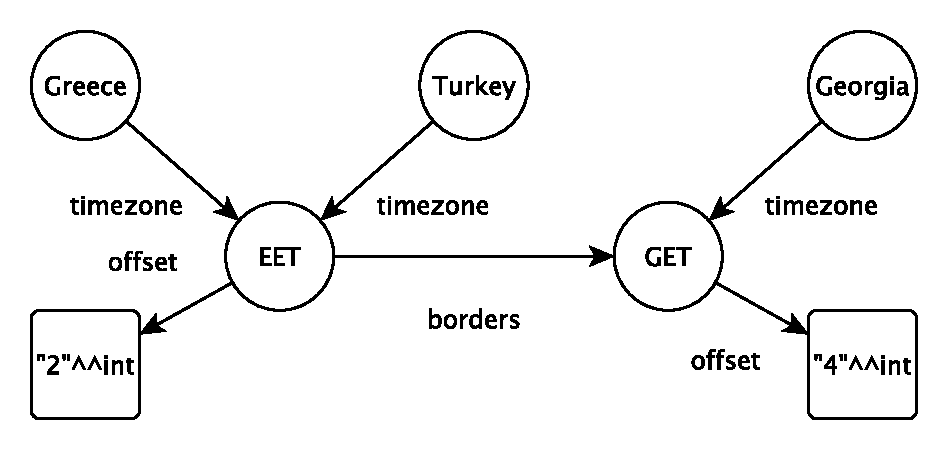
\includegraphics[width=\linewidth]{part_01/fig_graph.pdf}
\caption{Example of Linked Data used for the calender application.}
\label{fig:graph}
\end{figure}

The last two triples in the example graph demonstrate the use of literal values in the object position: instead of a named node, that refers to an entity, we have a typed literal value.
In this case, the type is \texttt{int} and thus values should be interpreted as integers.
The types available in \ac{RDF} include numbers, strings, booleans, dates, time durations, URIs, XML, and others.

\medskip

\textbf{Further readings}:
To deepen your knowledge w.r.t. the formalisms of \ac{RDF} you may read the \ac{RDF} specification~\cite{rdf-spec}, 
the \ac{RDF} primer~\cite{rdfprimer} or 
the specification for XSD datatype~\cite{xsd-part2}.
Relevant concepts we did not introduce are blank nodes, reification, named graphs and extensible datatypes~cf.~\cite{namedgraphs,rdfprimer}.

\section{URIs: The words of the language}
\label{uri}

The major advantage of a graph-based model is its ability to be merged by simply regarding a merger as a union of the triples in both graphs.
Many other models for knowledge representations, like tables or XML files, do not allow such a generic merging.
But in order to provide a knowledge representation language that allows these kind of mergers, naming conflicts must be avoided.
In contrast to our example above where \texttt{Georgia} refers to a caucasian country, consider a second \ac{KB} about U.S. states:

\begin{verbatim}
 Georgia timezone EST .
 SouthCarolina timezone EST .
 EST offset "-5"^^int .
\end{verbatim}

Since both Georgias -- the caucasian country and the U.S. state -- have the same name, we are not able to differentiate between them.
Georgia now seems to be both in the timezone \texttt{GET} and \texttt{EST}!

To avoid this situation, all entities in Linked Data have to be referred to by unique names.
To achieve this, the names are given as URIs, most often HTTP URIs (just like websites).
The main advantage of URIs is that anyone can register a prefix, and then create a set of new names with this prefix.
The owner of the prefix is responsible for the interpretation of the given name.
Thus, the country Georgia could be named \url{http://example.org/countries\#Georgia} and the U.S. state could be \url{http://example.org/usstates\#Georgia}.
The basic intuition behind the idea is that everyone can define their own namespace so that naming conflicts can be avoided without constant coordination between different parties.

As URIs can be lengthy, often qualified names (or \textit{QNames}) are used.
They have the form \texttt{prefix:localName}.
Prefixes are defined locally to expand to a certain namespace, e.g., in our example we could define that the prefix \texttt{us} refers to the namespace \url{http://example.org/usstates\#}, and thus we could use the qualified name \texttt{us:Georgia} to refer to the complete URI \url{http://example.org/usstates\#Georgia}.

\medskip

\textbf{Further readings}:
For deeper insights, please refer to the specification of URIs~\cite{uri} and the URI registration scheme~\cite{uri-registration}.
We did not cover IRIs~\cite{iri} and other protocols besides HTTP, like FTP~\cite{ftp} or URN~\cite{urn}.

\section{HTTP: Distributed knowledge}
\label{http}

The second rule for publishing Linked Data is to use HTTP URIs.
HTTP is a widely implemented protocol, that can be used over Internet for accessing resources with a given HTTP URI.
For example, the above \ac{KB} could have the name \url{http://example.org/countries}.
Now a simple HTTP command like 
\begin{verbatim}
GET http://example.org/countries
\end{verbatim}
will return the \ac{KB} (it can be tried by entering the URI in a browser, but it is suggested for later as the result might be confusing at this point).

All \ac{RDF} entities are identified by URIs, and the third rule of Linked Data demands to return information about the entity identified with a given URI when the URI is being dereferenced via HTTP.
This way, the Web can be used as vast knowledge space, where everyone can publish their knowledge about a given entity.

Since entities are uniquely identified, we can avoid to publish our own URIs for existing entities.
For example, DBpedia is a widely used resource that publishes Linked Data based on Wikipedia's infoboxes~\cite{dbpedia-swj}.
DBpedia offers URIs for all entities that have a Wikipedia page.
For example, Greece's Wikipedia page is \url{http://en.wikipedia.org/wiki/Greece} and, based on that, DBpedia defines the URI for Greece to be \url{http://dbpedia.org/resource/Greece}.
When entering the URI into a browser, the browser redirects the user to a Web page about Greece in DBpedia.
If a Semantic Web application would have asked, DBpedia (prefix dbpedia) would have returned the \ac{RDF} data instead.

So we could replace

\begin{verbatim}
 countries:Greece tz:timezone tz:EET .
\end{verbatim}

with using the DBpedia URI for Greece and get

\begin{verbatim}
 dbpedia:Greece tz:timezone tz:EET .
\end{verbatim}

Following the second Linked Data rule, we can enhance our knowledge about Greece: the name of the country in different languages and alphabets, its population, the name of the head of state, etc.
Thus, our application can use knowledge from all over the Web.

Instead of simply replacing the URI, in our case we actually state that the URIs refer to the same entity:

\begin{verbatim}
 countries:Greece owl:sameAs dbpedia:Greece .
\end{verbatim}

Note, properties can be reused from all over the Web.
In this case, we use the term \texttt{sameAs} from the OWL vocabulary~\cite{owl} which we will look at in the next section.

One advantage of using the Web as a \ac{KB} is that much knowledge is already published,
whereas our knowledge bases had information on some countries.
Websites like LinkedGeoData~\cite{linkedgeodata} or DBpedia offer lists of cities, and information about the countries or states they are located.
Regarding cities, the Web already offers the following pieces of knowledge:

\begin{verbatim}
 dbpedia:Istanbul dbo:country dbpedia:Turkey .
 dbpedia:Athens dbo:country dbpedia:Greece .
 dbpedia:Atlanta dbo:isPartOf dbpedia:Georgia_(U.S._state) .
\end{verbatim}

This allows to reuse the knowledge about cities from the Web of Data in a non-costly manner.

\medskip

\textbf{Further readings}:
For a deeper introduction of the HTTP protocol have a look at the HTTP specification~\cite{http}.

\section{RDFS, OWL and others: Adding expressivity}
\label{rdfs}

So far we have seen that \ac{RDF} allows us to express triples directly.
A very powerful method is the use of implicit triples by using more expressive semantics than simple triples.
We have introduced one example already: \texttt{owl:sameAs} states that two URIs refer to the same entity.
That is, anything we say about \texttt{dbpedia:Greece} is also true about \texttt{countries:Greece}.
We learnt that \texttt{dbpedia:Athens} is in \texttt{dbpedia:Greece}, thus we know that it is also in \texttt{countries:Greece}.

A number of languages are built on top of \ac{RDF} and extend it with more expressive semantics.
We will look at two of them, that are standardized by the W3C: RDFS and OWL. %, and RIF.

RDFS allows us to describe class and property hierarchies.
For example, we have found on the Web cities connected to countries, resp. U.S. states.
The connection to a country was done by using the property \texttt{dbo:country} and to the state by \texttt{dbo:isPartOf}.
Now, we can also define that everything that is connected via the former should also be connected through the latter.
With RDFS, it is expressed by:

\begin{verbatim}
 dbo:country rdfs:subPropertyOf dbo:isPartOf .
\end{verbatim}

Now a reasoner that follows the RDFS semantics can infer that

\begin{verbatim}
 dbpedia:Istanbul dbo:isPartOf dbpedia:Turkey .
\end{verbatim}

is true, even though it had never been stated explicitly.

OWL is much more expressive regarding the description of classes and properties.
For example, we can state that every city has to be in exactly one time zone or that no entity can be both a U.S. state and a country, which could have helped to discover the error with the two Georgias automatically.

Since \ac{RDF} allows only triples, more complex statements need to be dissolved into triples.
The statement \textit{"Every city is in exactly one time zone."} translates in \ac{RDF} to the following four triples:

\begin{verbatim}
x:statement1 rdf:type owl:Restriction .
x:statement1 owl:onProperty tz:timezone .
x:statement1 owl:qualifiedCardinality "1"^^xsd:nonNegativeInteger .
x:statement1 owl:onClass dbo:City .
\end{verbatim}

Although this might seem a bit daunting, in reality these kind of triples are hidden either by more high-level syntaxes (see Section~\ref{rdfa}) or query tools (see Section~\ref{sparql}).

%RIF is a different beast.
%Whereas OWL is an expressive language to describe classes and properties, RIF is a way to express rules of them form \textit{if\ldots{}then\ldots{}}.
%In our example, we might want to state that whenever a city is part of a country or state, and the country or state has a time zone, this is also the time zone of the city. Or, using the variables \texttt{?x}, \texttt{?y}, and \texttt{?z}:%
%\footnote{We will not show how the rule is represented in RDF, as this looks even worse than the OWL statement above.}
%
%If
%\begin{verbatim}
% ?x dbo:isPartOf ?y .
% ?y tz:timezone ?z .
%\end{verbatim}
%then
%\begin{verbatim}
% ?x tz:timezone ?z .
%\end{verbatim}

%RDFS, OWL, and RIF can, at least in theory, be all used together.
RDFS and OWL can be used together theoretically.
However, it depends on the used tools if a given semantics is understood: some reasoners support parts of OWL (so called fragments), some support only RDFS and a very few claim to support interesting combinations of all three languages (including the RIF Rule language), and sometimes beyond.

\medskip

\textbf{Further readings}:
Full formalism can be found in the specifications for RDFS~\cite{rdfs}, OWL~\cite{owl}, and RIF~\cite{rif}.
%We did not discuss questions of how to reason and about the complexity and decidability of reasoning. 
%This is a big research topic, and in the last few years, it was advanced tremendously. 
We point to the DL Handbook as an entry point into this topic~\cite{dl-handbook}.
We also did not mention the different fragments of OWL, RIF, and the differences between OWL and OWL2, which can all be found in detail in the respective standards.
Besides the languages presented here, other languages like SKOS~\cite{skos} or WSML~\cite{wsml} exist, that can define other semantics.

\section{SPARQL: Querying RDF}
\label{sparql}

So far, we have described how to express knowledge: simple facts (with \ac{RDF}) and more expressive statements that enrich the \ac{KB} (in the previous section).
SPARQL provides a structured query language for \ac{RDF} knowledge bases.

For example, assume that all the triples mentioned so far are in one graph that can be queried via SPARQL.
Assume also that the system providing the SPARQL endpoint interprets the semantics of RDFS, OWL, and RIF.
Now we can retrieve the time offset for Athens as follows:

\begin{verbatim}
 SELECT ?offset WHERE {
   dbpedia:Athens tz:timezone ?tz .
   ?tz tz:offset ?offset .
 }
\end{verbatim}

The system will return as a result the integer $2$.
The web provides us with the data that Athens is a city located in the country Greece.
Due to the OWL sub-property triple, we also know that to be in a country means to be part of it.
Because of the RIF rule, we can infer that if something is part of something else, it also has the same timezone.
Based on this, the following two triples, the first one implicitly, the second given explicitly, are in our \ac{KB}:

\begin{verbatim}
 dbpedia:Athens tz:timezone tz:EET .
 tz:EET tz:offset "2"^^xsd:int .
\end{verbatim}

A SPARQL query describes a triple pattern (similar to the one in the \textit{if}-part of RIF),
where symbols with a leading question mark are variables.
A SPARQL processor now tries to find values for the variables, so that the whole SPARQL pattern can be fulfilled by the \ac{KB}.
The SPARQL processors then returns a list of all possible answers for the selected variables, i.e., in this case for all values that \texttt{?offset} can have so that the SPARQL query pattern matches in the \ac{KB}.
That is, all variables following the introductory \texttt{SELECT} keyword, in this case \texttt{?offset}.

Given our query pattern, the two triples above are the only match in our \ac{KB}, and thus the result, \texttt{"2"\texttt{\char`\^}\texttt{\char`\^}xsd:int } will be returned as the only possible value for \texttt{?offset}.

SPARQL can be regarded as the main interface for machines to access knowledge on the Web of Data.
The usual workflow to query Linked Data is to find and gather trustworthy data from the Web, include some knowledge created for the task or tying together the data from the Web, put it all in one \ac{KB}, and then use SPARQL to get answers to the queries of interest to the given task.
Currently, we observe an upcoming trend of natural language interfaces to provide also laymen the possibility to access the Web of Data without knowing any of the underlying systems, see~\url{https://www.w3.org/community/nli/}.

\medskip

\textbf{Further readings}:
To find out more about SPARQL look at the specification for SPARQL~\cite{Sparql11query}.
We did not discuss that SPARQL is not only a query language but also a protocol of how to acccess SPARQL endpoints.
We also did not discuss other types of queries: \texttt{DESCRIBE}, \texttt{ASK}, and \texttt{CONSTRUCT}, nor the powerful features of SPARQL to count, do math, regular expressions, named graphs, etc.

\section{Serializations of RDF}
\label{rdfa}
What is a serialization?
In order to provide \ac{RDF} graphs through the Web, we need to serialize them in a sequence of tokens.
Throughout this chapter, we have used a slightly simplified, triple-based serialization, N3~\cite{n3-tech}.
N3 has the advantage, that the triple structure of the graph can be easily inferred.
Although, it is widely used, it has the disadvantage of not being standard.

There are a number of serializations of \ac{RDF} around, mostly due to the fact that the originally standardized serialization in RDF/XML is considered to be not very convenient.
Soon, further syntaxes were created, some of them also in XML (like TriX~\cite{trix}) or in even novel formats like N3 and its constrained version N-Triples~\cite{ntriples}.
Expressions in other languages like OWL and RIF are often hard to translate to \ac{RDF} (as shown in Section~\ref{rdfs}), and thus introduced serializations of their own, like the OWL Functional Syntax~\cite{owl2}, the OWL XML presentation syntax (a serialization of OWL directly in XML, instead of going through \ac{RDF}~\cite{owl3}), the RIF syntaxes~\cite{rif}, etc.
Lately, JSON-LD became a more prominent serialization format on the Web, and standards to represent the \ac{RDF} data model in JSON are being worked on~\cite{json-ld}.

%Besides serializations for pure RDF, there has been a second strand of embedding RDF in other file formats.
%One of the main use cases for RDF is to provide flexible metadata about a file.
%Embedding that metadata in the file itself has the advantage that the metadata is easier retained if the file gets moved, shared, changed, etc.
%A growing number of file formats, like Adobe's (PDF, Photoshop, etc.) allow to embed RDF~\cite{xmp}.

%The most relevant file format for the Web is obviously HTML itself, the language to describe Web pages and applications.
%The RDFa standard offers how to markup and annotate elements of a Web page with RDF.
%This allows a tool understanding RDFa to directly extract structured data out of a Website:
%a page about an event can be pulled into a calendar,
%a restaurant can be automatically filtered with the allergies of the user,
%different shopping Websites can be thrown into one \ac{KB} and be compared directly, etc.

\medskip

\textbf{Further readings}:
If you want to find more serializations have a look at the specifications of RDFa~\cite{rdfa}, RDF in JSON~\cite{json-ld}, and RDF/XML~\cite{rdfxml}.
Also relevant is the ongoing conversation between the communities supporting Microformats~\cite{microformats}, Microdata~\cite{microdata}, and RDFa.

%\section{XML: The confusing older brother}
%\label{xml}
%
%XML became the de-facto lingua france for data on the Web and beyond.
%So it was natural, that it was assumed that RDF would be build on top of XML.
%But in reality, the two are very different beasts:
%XML describes a tree-based model, with a single root element, that has child elements in a strict order, and, who in turn, might have further child elements, in strict orders too, all strictly hierarchical.
%RDF describes a graph-based model, where the order of the edges does not matter, and that is expressed as a simple set of triples.
%XML schema defines a strict grammar for the elements in an XML documents, determining if an XML file is valid or not.
%RDF schemas provide additional knowledge to infer implicit knowledge from a given RDF file, and can hardly be used to check the validity of an RDF file.
%It is often easier to deal with valid XML files than with RDF files, because the developer has guarantees about the structure of the file.
%On the other hand, RDF files are much easier to extend: one can simply add further triples, and, as long as they don't contradict the existing triples, the knowledge simply grows.
%Two RDF files can always be simply merged automatically. For XML files in general, such an operation makes no sense.
%
%With the benefit of hindsight, forcing RDF into an XML-based serialization was bound to lead to numerous problems without gaining the hoped-for advantages.
%Many of the existing XML tools and workflows were actually unable to deal with RDF/XML files, so that the existing huge pool of experience and software could not be used to kickstart the Web of Data.
%
%Today, XML does not play a prominent role for the Web of Data anymore.
%Even if it gets further used as the main serialization format for RDF, its data model and the tools used with XML are loosing relevance.
%It is an open question if this might change again, or if the rich set of software and experiences surrounding the XML world can be unlocked in favor of the Web of Data -- or the other way around.
%
%\medskip
%
%\textbf{Further readings}:
%For more information about XML, see the XML specification~\cite{xml} or the XML Schema primer~\cite{xml-primer}.

\section{Conclusions and outlook}
\label{conclusions}

\ac{RDF} is increasingly becoming the standard way to share data on the Web, especially in embedded-HTML formats\footnote{\url{https://www.similartech.com/categories/schema}}.
Using and publishing \ac{RDF} is not an academic privilege anymore.
The flexibility and extensibility of \ac{RDF}, along with the possibility to merge arbitrary \ac{RDF} graphs, gives it a unique advantage compared to other wide spread data models.
The plurality of serializations, especially the ill-received standard RDF/XML-serialization, a over-emphasized focus on OWL, and the delayed availability of SPARQL hindered the early growth of \ac{RDF}.
Meanwhile, simple standards, like Microformats and JSON-LD, have received considerable uptake.

The advantages and the availability of Linked Data standards are being increasingly recognized.
Instead of introducing hundreds of APIs and heterogeneous formats, one common data model and query language can substantially decrease costs of data integration and data reuse.
Thus, recent approaches such as Triplify~\cite{triplify_www}, D2R~\cite{Bizer04} and SPARQLMap~\cite{unbehauen-jist-2012-sparqlmap} try to built a \ac{RDF} layer on top of heterogeneous data sources.

End user interfaces to the Web of Data are still limited.
%$Maybe the role of Linked Data is to be background technology:
%no one asks for generic interfaces for end-users to SQL databases.
%Maybe the Web of Data has a similar fate.
However, the uptake of Linked Data and its combination with novel, powerful natural language technologies -- like hybrid question answering, c.f. Part~\ref{part:hybridQA} -- allows the implementation of end user interfaces without the need to know the underlying standards or mechanisms.
Thus, laymen and professional users can benefit from the wealth of knowledge rising from the Semantic Web implementation.

Still several practical issues remain unresolved:
\begin{itemize}
%\item In general, SPARQL is too powerful and too expensive for the Web. It is far too easy to bring a SPARQL endpoint down with a few queries.
\item The multitude of serialization formats in practical use combined with the lack of standard formats besides RDF/XML hampers teaching about \ac{RDF} and its uptake.
\item For a number of wide-spread use cases, no standards or widely accepted practices exists: how to express numbers with units, especially imperial units? How to express data that was valid at a given point in time? %How to express time spans? How to deal with numerical precision? How to work with simple geographical and temporal reasoning, like inclusion?
%\item Currently, most standards allow fine-grained provenance information only through reification, a method, that is often strongly discouraged for several reasons.
\item The semantics can break down under inconsistencies. There is currently no accepted way to deal with diversity in knowledge bases, even though this will play a crucial role on the Web. This ties in with questions of trust that have not yet been sufficiently tackled: given diverse data about an entity, maybe even contradictions, how to choose which sources to trust? %How to make this trust transferable to the user?
\end{itemize}

The Web of Data, as part of the Web, is getting increasingly tangled with all aspects of our lives.
The growing number of intelligent apps and devices in our environment will have an ever-growing need to communicate with each other.
Imagining a future where our calendar app can support the flight finder app by restricting the departure and arrival times based on our agenda and the locations of our meetings and the airport, has become much easier today than it used to be only a few years ago.
Such a future is much easier to achieve when the applications and devices can all communicate in the same common and standard data model, and using the same interfaces.


\todo[inline]{check for acronyms}
\chapter{Related Work}
%%%%%%%AGDISTIS
\section{Related Work}
\label{sec:relatedwork}
AGDISTIS is related to the research area of Information Extraction~\cite{nad:sek} in general and to \ac{NED} in particular.
Several approaches have been developed to tackle \ac{NED}. 
Cucerzan presents an approach based on extracted Wikipedia data towards disambiguation of named entities~\cite{Cucerzan07}.
The author aims to maximize the agreement between contextual information of Wikipedia pages and the input text by using a local approach.
%\todo{What's a local approach?}
\emph{Epiphany}~\cite{epiphany} identifies, disambiguates and annotates entities in a given HTML page with RDFa. 
Ratinov et al.~\cite{rat:rot} described an approach for disambiguating entities from Wikipedia. 
The authors argue that using Wikipedia or other ontologies can lead to better global approaches than using traditional local algorithms which disambiguate each mention separately using,\,e.g., text similarity. %for word sense disambiguation.
Kleb et al.~\cite{Kleb11WIMS,KlebESWC10} developed and improved an approach using ontologies to mainly identify geographical entities but also people and organizations in an extended version. 
These approaches use Wikipedia and other Linked Data \ac{KB}s.
LINDEN~\cite{LINDEN} is an entity linking framework that aims at linking identified named entities to a knowledge base.
To achieve this goal, LINDEN collects a dictionary of the surface forms of entities from different Wikipedia sources, storing their count information.

Wikipedia Miner~\cite{milne2008learning} is the oldest approach in the field of \emph{wikification}.
Based on different machine learning algorithms, the systems disambiguates w.r.t. prior probabilities, relatedness of concepts in a certain window and context quality. 
The authors evaluated their approach based on a Wikipedia as well as an AQUAINT subset. 
Unfortunately, the authors do not use the opportunities provided by Linked Data like DBpedia.

Using this data the approach constructs candidate lists and assigns link probabilities and global coherence for each resource candidate.
The AIDA approach~\cite{AIDA} for \ac{NED} tasks is based on the YAGO2 \ac{KB} and relies on sophisticated graph algorithms. 
Specifically, this approach uses dense sub-graphs to identify coherent mentions using a greedy algorithm enabling Web scalability. 
Additionally, AIDA disambiguates w.r.t.~similarity of contexts, prominence of entities and context windows.

Another approach is DBpedia Spotlight~\cite{spotlight}, a framework for annotating and disambiguating Linked Data Resources in arbitrary texts.
In contrast to other tools, Spotlight is able to disambiguate against all classes of the DBpedia ontology.
Furthermore, it is well-known in the Linked Data community and used in various projects showing its wide-spread adoption.\footnote{\url{https://github.com/dbpedia-spotlight/dbpedia-spotlight/wiki/Known-uses}}
Based on a vector-space model and cosine similarity DBpedia Spotlight is publicly available via a web service\footnote{\url{https://github.com/dbpedia-spotlight/dbpedia-spotlight/wiki/Web-service}}.

In 2012, Ferragina et al. published a revised version of their disambiguation system called TagMe 2.
The authors claim that it is tuned towards smaller texts,\,i.e., comprising around 30 terms.
TagMe 2 is based on an anchor catolog (\texttt{<a>} tags on Wikipedia pages with a certain frequency), a page catalogue (comprising all original Wikipedia pages,\,i.e., no disambiguations, lists or redirects) and an in-link graph (all links to a certain page within Wikipedia).
First, TagMe 2 identifies named entities by matching terms with the anchor catalog and second disambiguates the match using the in-link graph and the page catalog via a collective agreement of identified anchors. 
Last, the approach discards identified named entities considered as non-coherent to the rest of the named entities in the input text.  

In 2014, Babelfy~\cite{babelfy} has been presented to the community.
Based on random walks and densest subgraph algorithms Babelfy tackles \ac{NED} and is evaluated with six datasets, one of them the later here used AIDA dataset. 
In constrast to AGDISTIS, Babelfy differentiates between word sense disambiguation, i.e., resolution of polysemous lexicographic entities like \emph{play}, and entity linking, i.e., matching strings or substrings to knowledge base resources.
Due to its recent publication Babelfy is not evaluated in this paper.

Recently, Cornolti et al.~\cite{cornolti} presented a benchmark for \ac{NED} approaches.
The authors compared six existing approaches, also using DBpedia Spotlight, AIDA and TagMe 2, against five well-known datasets. % on different tasks and with different measures.
Furthermore, the authors defined different classes of named entity annotation task, e.g. \emph{`D2W'}, that is the disambiguation to Wikipedia task which is the formal task AGDISITS tries to solve.
We consider TagMe 2 as state of the art w.r.t. this benchmark although only one dataset has been considered for this specific task.
%We analyze the performance of DBpedia Spotlight, AIDA, TagMe 2 and our approach AGDISTIS on four of the corpora from this benchmark in Section~\ref{sec:eval}.

%%%%%%%GERBIL

\section{Related Work}
Named Entity Recognition and Entity Linking have gained significant momentum with the growth of Linked Data and structured knowledge bases. Over the last few years, the problem of result comparability has thus led to the development of a hand full of frameworks.

The BAT-framework~\cite{cornolti} is designed to facilitate the benchmarking of named entity recognition (NER), named entity disambiguation (NED) -- also known as linking (NEL) -- and concept tagging approaches.
BAT compares seven existing entity annotation approaches using Wikipedia as reference.
%Cornolti et al. were not able to compare CMNS and CSAW due to unavailable source code. \todo[inline]{is the software still unavailable?}
Moreover, it defines six different task types, five different matchings and six evaluation measures providing five datasets.
% which we will explain in Section~\ref{sec:architecture}.
%(Giuseppe) should this go here?
Rizzo et al.~\cite{rizzo2014}  present a state-of-the-art study of NER and NEL systems for annotating newswire and micropost documents using well-known benchmark datasets, namely CoNLL2003 and Microposts 2013 for NER as well as AIDA/CoNLL and Microposts2014~\cite{Cano2014} for NED. 
%The systems analyzed in this study are the ones supported by the NERD Framework~\cite{rizzo2012}, with the addition of the Stanford NER toolkit~\cite{StanfordNER}.
%Different systems use different schemas for entity typing and different knowledge bases for entity disambiguation. 
The authors propose a common schema, named the NERD ontology\footnote{\url{http://nerd.eurecom.fr/ontology}}, to align the different taxonomies used by various extractors. To tackle the disambiguation ambiguity, they propose a method to identify the closest DBpedia resource by (exact-)matching the entity mention.

Over the course of the last 25 years several challenges, workshops and conference dedicated themselves to the comparable evaluation of information extraction (IE) systems. 
Starting in 1993, the Message Understanding Conference (MUC) introduced a first systematic comparison of information extraction approaches~\cite{Sundheim:1993:TIE:1072017.1072023}.
Ten years later, the Conference on Computational Natural Language Learning (CoNLL) started to offer a shared task on named entity recognition and published the CoNLL corpus~\cite{conll2003}.
In addition, the Automatic Content Extraction (ACE) challenge~\cite{doddington2004automatic}, organized by NIST, evaluated several approaches but was discontinued in 2008. 
Since 2009, the text analytics conference hosts the workshop on knowledge base population (TAC-KBP)~\cite{mcnamee2009overview} where mainly linguistic-based approaches are published.
The Senseval challenge, originally concerned with classical NLP disciplines, has wided it focus in 2007 and changed its name to SemEval to account for the recently recognized impact of semantic technologies~\cite{kilgarri1998senseval}.
The Making Sense of Microposts workshop series (MSM) established in 2013 an entity recognition and in 2014 an entity linking challenge thereby focusing on tweets and microposts~\cite{MSM2014}.
In 2014, Carmel et al.~\cite{ERD2014} introduced one of the first Web-based evaluation systems for NER and NED and the centerpiece of the entity recognition and disambiguation (ERD) challenge. Here, all frameworks are evaluated against the same unseen dataset and provided with corresponding results. 

GERBIL goes beyond the state of the art by extending the BAT-framework as well as~\cite{rizzo2014} in several dimensions to enhance reproducibility, diagnostics and publishability of entity annotation systems. In particular, we provide \numberOfadditionalDatasets additional datasets and \numberOfadditionalAnnotators additional annotators. The framework addresses the lack of treatment of NIL values within the BAT-framework and provides more wrapping approaches for annotators and datasets. Moreover, GERBIL provides persistent URLs for experiment results, unique URIs for frameworks and datasets, a machine-readable output and automatic dataset updates from data portals. Thus, it allows for a holistic comparison of existing annotators while simplifying the archiving of experimental results. Moreover, our framework offers opportunities for the fast and simple evaluation of entity annotation system prototypes via novel NIF-based~\cite{NIF} interfaces, which are designed to simplify the exchange of data and binding of services.
%Additionally, each configured experiment has its own persistent and publishable URI to enable reproducible research at web-scale, .
%Figure~\ref{fig:architecture} gives an overview of GERBILs components, interaction possibilities and data streams.
%\todo[inline]{AnBo: The paragraph sounds a lot like buzzwording with few concret information. I suggest to stick to the MVC pattern and describe what is the view here, what is the model, how are these components addressing the outcome of the related work. What are the disadvantages of the previous approaches. I would prefer that we add a related work section (the above paragraph should be the core of this section). Axel: Done}

%The main drawback is that this evaluation was done for one single dataset (that of the ERDchallenge). Moreover, the challenge organizers decided not to publish the gold standard of their dataset to make the evaluation more independent and not let participants build system to solve the problem on their dataset thus losing generality. (marco) Done. (Axel)}
%\todo[inline]{Wo sollten wir sagen dass wir uns aus Rechenlastgründen nur auf webservices beschränken? Intro?}

%%%%%%%QA
\section{Question Answering}


\part{Knowledge Extraction}
%\cleardoublepage
\ctparttext{
    The second part 
}
\chapter[$\mbox{N}^3$ - A Collection of Datasets for NER and NED in NIF]{$\mbox{N}^3$ - A Collection of Datasets for Named Entity Recognition and Disambiguation in the NLP Interchange Format}
\label{cha:N3}
\graffito{
This chapter presents $\mbox{N}^3$, a collection of three annotated corpora for \ac{NER} and \ac{NED}.,
It has been published in~\cite{n3} and since than build the gold standard for evaluations in papers like \cite{agdistis_iswc, GERBIL}.
The author of this thesis is one of the two main authors, implemented the annotation tool, generated parts of the datasets and co-wrote the paper and its poster. 
}
\lstset{
  basicstyle=\footnotesize\ttfamily,
  breaklines=true,
  captionpos=b,                    % sets the caption-position to bottom
  frame=single,
  %morecomment=[s][\color{blue}]{<}{>},
  morecomment=[s][\color{red}]{"}{"},
  numbers=none  
%  numbersep=5pt,
% numberstyle=\tiny,
%  stringstyle=\tiny
}
%\name{Michael R{\"o}der$^{1,2,\star}$, Ricardo Usbeck$^{1,2,\star}$, Sebastian Hellmann$^{1}$, Daniel Gerber$^1$ \& Andreas Both$^{1,2}$}
%\institute{First Institute Name \email{email address} \and Second Institute Name\thanks{Thank you to...} \email{email address}}
%\address{
%$^{1}$ Agile Knowledge Engineering and Semantic Web, University Leipzig, Germany \\
%$^{2}$ R\,\&\,D, Unister GmbH, Germany}

%\abstract{
%Extracting Linked Data following the Semantic Web principle from unstructured sources has become a key challenge for scientific research. % as well as new business models. \todo{Jens: Which business models? This just appears in the abstract and not the introduction.}
%Named Entity Recognition and Disambiguation are two basic operations in this extraction process.
%%\todo{Jens: maybe "One step towards the realization of ..." - avoid repeating "key driver"} 
%One step towards the realization of the Semantic Web vision and the development of highly accurate tools is the availability of data for validating the quality of processes for Named Entity Recognition and Disambiguation as well as for algorithm tuning.
%This article presents three novel, manually curated and annotated corpora ($\mbox{N}^3$). All of them are based on a free license and stored in the NLP Interchange Format to leverage the Linked Data character of our datasets. %\todoanbo{make more catchy} % for interoperability reasons.
%\\ \newline \Keywords{Datasets, NLP Interchange Format, Named Entity Detection, Named Entity Disambiguation}
%}

%\maketitleabstract

%\section{Introduction}

Automatically extracting and linking Named Entities (NEs) to a particular \ac{KB}  from unstructured, natural language text is an extremely challenging task~\cite{Cucerzan07}. 
Leveraging Linked Data can help developing tools to automatically extract semantic data~\cite{GER+13,AIDA,spotlight,agdistis_iswc}.

The tasks of \ac{NER}  and \ac{NED}  are part of the research area of Information Extraction~\cite{FOX}.
NER is the task of identifying entities of certain types.
%why not use the NERD core classes? 
NED is the task of disambiguating pre-identified named entities towards a certain \ac{KB} .
%NED is based on pre-identified named entities and their disambiguation towards a certain KB. %using various methods.
%RE determines links between entities based on a given context leading to Information Extraction~\cite{fox}.
These IE steps depend on datasets which need human annotation, and therefore make it a time-consuming and expensive task.
Approaches like AGDISTIS (Chapter~\ref{cha:agdistis}) or CETUS (Chapter~\ref{cha:cetus}) need to be evaluated against high-quality, easily deployable and diverse datasets.
%\todo[inline]{Why does RE lead to IE? This formulation seems a little bit strange and does not really fit to the next sentence in which RE is a step of IE.}
%\todo[inline]{Done, but does it really fit in here? (rewrite that section, mention that NED is done by using DBpedia as KB. DBpedia is the central point of the Linked Open Data movement.)}

Thus, we present three novel datasets (called $\mbox{N}^3$) in which named entities have been annotated manually. As \ac{KB}  for this annotation we used DBpedia~\cite{dbpedia-swj} which is the central point of the Linked Open Data movement. These datasets have already been used to evaluate~\cite{AIDA,spotlight} as well as in~\cite{GER+13,agdistis_iswc,GERBIL}.
$\mbox{N}^3$ is published using the \ac{NLP} Interchange Format (NIF)~\cite{ISWC2013NIF} ensuring a greater interoperability to overcome the need for corpus-specific parsers. 
Our main contributions are as follows:
\begin{itemize}
\item The publication of three novel and freely available datasets for \ac{NER} and \ac{NED};
\item An analysis of the underlying corpora;
\item The transformation of these corpora to NIF providing provenance data.
\item Finally, our datasets also allow the analysis of coreference resolution~\cite{NgongaNgomo2014,singh} if the entity is not in the \ac{KB}  of the respective corpus.
\end{itemize}
The data as well as further information can be found at the project homepage \url{http://aksw.org/Projects/N3nernednif}.


\section{Corpora}
\label{n3:sec:Features}




In the following section, we present the annotation process as well as specific features for each corpus of the $\mbox{N}^3$-Collection.

During the annotation, we focused on recognizing three main classes of NEs: persons, places and organizations. 
Each identified NE has been manually disambiguated to the DBpedia 3.9  if possible.
In case there was no matching resource from a \ac{KB}  we created an URI\footnote{\url{http://www.w3.org/TR/cooluris/}} using the \url{http://aksw.org/notInWiki/} namespace (see Section~\ref{n3:NIF}).
Additionaly, we resolved coreferences for every named entity, especially, for entities that are not yet in the \ac{KB} . %\todo[inline]{coreference resolved?}

Furthermore, the collection of datasets is annotated by the version and language of the \ac{KB} , hence any change of the underlying database can be analysed.
In order to spread the corpora, we publish them under the Creative Commons BY-NC-SA license\footnote{\url{http://creativecommons.org/licenses/by-nc-sa/4.0/}}.

In general, our corpora contain more documents then any published NIF corpora (\texttt{KORE50} and \texttt{DBpedia Spotlight}) so far.
First order statistics for all datasets, such as the number of documents, words or average word count per document, can be found in Table~\ref{n3:tab:corpus_stats}.
Moreover, Table~\ref{n3:tab:entity_counts} describes the number of entities and URIs known or not known in DBpedia w.r.t. a certain dataset.


\begin{table}[htb!]
	\centering
	\resizebox{\textwidth}{!}{
    \begin{tabular}{lp{0.0cm}cp{0.0cm}D{.}{}{3.0}p{0.0cm}D{.}{}{5.0}p{0.0cm}D{.}{.}{4.2}}
     \toprule
     \textbf{Corpus} && \textbf{Language} && \multicolumn{1}{c}{\textbf{\#Documents}} && \multicolumn{1}{c}{\textbf{\#Words}} && \multicolumn{1}{c}{\textbf{Avg. Words/Doc.}} \\
    \midrule
    News-100 && German && 100 && 48199 && 481.99 \\
	Reuters-128 && English && 128 && 33413 && 261.04 \\
	RSS-500 && English && 500 && 31640 && 63.28 \\
    \midrule
    KORE50 && English && 50 && 1332 && 26.64 \\
    DBpedia Spotlight && English && 10 && 3582 && 358.20 \\
	\bottomrule
	\end{tabular}}
	\caption{Features of the corpora and their documents.}
	\label{n3:tab:corpus_stats}
\end{table}

\begin{table}[htb!]
	\centering
    \begin{tabular}{lp{0.25cm}D{.}{}{4.0}p{0.25cm}D{.}{}{4.0}p{0.25cm}D{.}{}{4.0}p{0.25cm}D{.}{}{4.0}}
     \toprule
	 \multirow{2}{*}{\textbf{Corpus}} && \multicolumn{3}{c}{\textbf{Entities}} && \multicolumn{3}{c}{\textbf{Unique URIs}}\\
	  && \multicolumn{1}{c}{\textbf{DBpedia}} && \multicolumn{1}{c}{\textbf{AKSW}} && \multicolumn{1}{c}{\textbf{DBpedia}} && \multicolumn{1}{c}{\textbf{AKSW}} \\
	\midrule
	News-100 && 1547 && 108 && 315 && 57 \\
	Reuters-128 && 650 && 230 && 299 && 145 \\
	RSS-500 && 524 && 476 && 400 && 449 \\
    \midrule
    KORE50 && 144 && 0 && 127 && 0 \\
    DBpedia Spotlight && 331 && 0 && 249 && 0 \\
	\bottomrule
	\end{tabular}
	\caption{Number of single entities and unique URIs in the corpora.}
	\label{n3:tab:entity_counts}
\end{table}


The distribution of NEs over the texts is shown in Figure \ref{n3:fig:nePerDoc}. 
\begin{figure}[htb!]
  \centering
  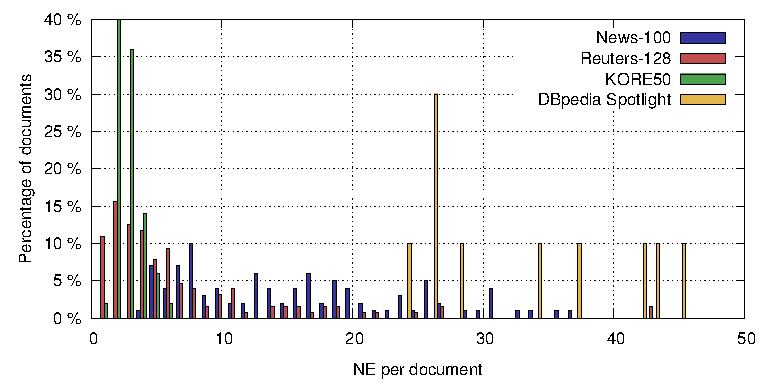
\includegraphics[width=\linewidth]{part_02/benchmarking/LREC_N3NIFNERNED/NE_per_doc.pdf}
  \caption{Distribution of NEs per document. We omitted two outliers from the News-100 corpus containing 55 and 63 NEs.}
  \label{n3:fig:nePerDoc}
\end{figure}

\texttt{RSS-500} has been left out because all of its documents comprise exactly two entities. 
As depicted in the diagram, all documents of the \texttt{KORE50} corpus have less than six NEs. 
The documents from \texttt{DBpedia Spotlight} corpus reveal a larger context and thus more NEs. 
On the other side, \texttt{DBpedia Spotlight} comprises only 10 documents.
The \texttt{Reuters-128} corpus has most documents, although many of these documents are shorter and thus have less NEs.



\subsection{News-100}

This corpus comprises 100 German news articles from the online news platform news.de\footnote{\url{http://www.news.de}}. 
All of the articles were published in the year of 2010 and contain the word \emph{Golf}.
This word is a homonym that can have the following meanings:
\begin{itemize}
\item A gulf like the Gulf of Mexico or the Persian Gulf,
\item The ball sport or
\item A car model produced by the German manufacturer Volkswagen.
\end{itemize}

One researcher annotated the documents manually.
Another researcher resolved occurring conflicts after supervising the corpus.
Although the sport golf as well as the car are not within the class range of NER, they are kept for evaluation purposes.

\subsection{Reuters-128}

This English corpus is based on the well known Reuters-21578\footnote{\url{http://kdd.ics.uci.edu/databases/reuters21578/reuters21578.html}} corpus which contains economic news articles.
In particular, we chose 128 articles containing at least one NE, as described in~\cite{agdistis_iswc}.
Compared to the \texttt{News-100} corpus the documents of \texttt{Reuters-128} are significantly shorter and thus carry a smaller context, as can be seen in Table \ref{n3:tab:corpus_stats}.

To create the annotation of NEs with URIs, we implemented a supporting judgement tool, see Figure~\ref{n3:fig:qrtool}\footnote{\url{https://github.com/RicardoUsbeck/QRTool}}. 
The input for the tool was a subset of more than 150 Reuters-21578 news articles sampled randomly.
First, FOX~\cite{FOX} was used for recognizing a first set of NEs. 
This reduced the amount of work to a feasible portion regarding the size of this dataset.

Afterwards, the domain experts corrected the  mistakes of FOX manually using the annotation tool.
Therefore, the tool highlighted the entities in the texts and added initial URI candidates via simple string matching algorithms.
Two scientists determined the correct URI for each named entity manually with an initial voter agreement of 74\%.
This low initial agreement rate hints towards the difficulty of the disambiguation task.

In some cases, judges did not agree initially but came to an agreement shortly after reviewing the cases.
While annotating, we left out ticker symbols of companies, e.g., \textit{GOOG} for Google Inc., abbreviations and job descriptions because those are always preceded by the full company name respectively a person's name.

\begin{figure}[htb!]
\centering
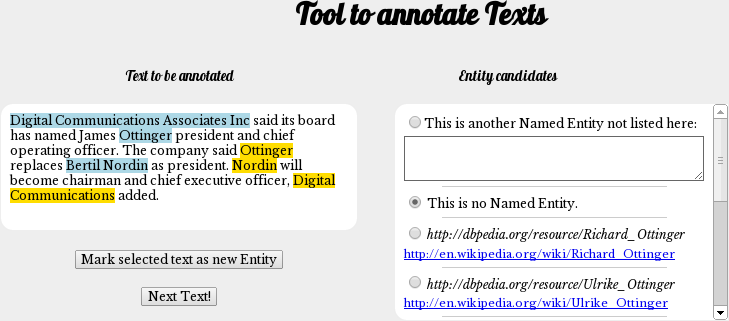
\includegraphics[width=\linewidth]{part_02/benchmarking/LREC_N3NIFNERNED/qrtool.png}
\caption{User interface of the annotation tool.}
\label{n3:fig:qrtool}
\end{figure}


\subsection{RSS-500}

This corpus has been created using a dataset comprising a list of 1,457 RSS feeds as compiled in~\cite{GOLDHAHN12.327}.
The list includes all major worldwide newspapers and a wide range of topics, e.g., \emph{World}, \emph{U.S.}, \emph{Business}, \emph{Science} etc.
The RSS list has been compiled using a 76-hour crawl, which resulted in a corpus of about 11.7 million sentences.
A subset of this corpus has been created by randomly selecting 1\% of the contained sentences.
 
Finally, one researcher annotated 500 randomly chosen sentences manually.
These sentences were a subset of those which contained a natural language representation of a formal relation, like ``\ldots, who was born in\ldots '' for \texttt{dbo:birthPlace}, cf.~\cite{conf/ekaw/GerberN12}.
The relations had to occur more than 5 times in the 1\% corpus. % with DBpedia URIs.
In case the mentioned entity is not contained in a new URI has been generated.
This corpus has been used for evaluation purposes in~\cite{GER+13}.

\section{Using NIF for publishing corpora}
\label{n3:NIF}



\begin{figure}[htb!]
\begin{lstlisting}[label=n3:TripleExampleNIF,caption=Example of the resulting N3-triples.]{TripleExampleNIF}
@prefix nif:     <http://persistence.uni-leipzig.org/nlp2rdf/ontologies/nif-core#> .
@prefix itsrdf:  <http://www.w3.org/2005/11/its/rdf#> .
@prefix xsd:     <http://www.w3.org/2001/XMLSchema#> .

<http://aksw.org/N3/Reuters-128/1#char=0,337>
      a       nif:String , nif:Context , nif:RFC5147String ;
      nif:beginIndex "0"^^xsd:int ;
      nif:endIndex "337"^^xsd:int ;
      nif:isString "Key Tronic corp said it has received contracts..."@en ;
      nif:sourceUrl <http://www.research.att.com/~lewis/Reuters-21578/15003> .

<http://aksw.org/N3/Reuters-128/1#char=0,15>
      a       nif:String , nif:RFC5147String ;
      nif:anchorOf "Key Tronic corp"^^xsd:string ;
      nif:beginIndex "0"^^xsd:int ;
      nif:endIndex "15"^^xsd:int ;
      nif:referenceContext  <http://aksw.org/N3/Reuters-128/1#char=0,337> ;
      itsrdf:taIdentRef <http://dbpedia.org/resource/Key_Tronic> ;
      itsrdf:taSource "DBpedia_en_3.9"^^xsd:string .
\end{lstlisting}
\end{figure}




For publishing our datasets, we choose NIF because it is a \ac{RDF}-based Linked Data serialization.
NIF provides different advantages, e.g., \emph{interoperability by standardization}~\cite{ISWC2013NIF} or \emph{query-ability}.
The \emph{NIF-standard} assigns each document an URI as starting point and generates another \ac{LD}  resource per NE.
Each document is a resource of type \texttt{nif:Context} and its content is the literal of its \texttt{nif:isString} predicate. 
Where possible, we added the source from which we got the document using the \texttt{nif:sourceUrl} predicate.
%where possible, the source from which the document was added used...predicate....
Every NE is an own resource with a newly generated URI pointing to the original document via the \texttt{nif:referenceContext} predicate.
Additionally, the begin (\texttt{nif:beginIndex}) and end position (\texttt{nif:endIndex}) as well as the disambiguated URI (\texttt{itsrdf:taIdentRef}) and the respective \ac{KB}  (\texttt{itsrdf:taSource}) are stored.
In contrast to Steinmetz~et~al.~\cite{steinmetz-n-2013-statistical}, mentioning the source of annotation serves as a more useful semantic background and is thus more valuable for further research.
For instance, NIF document as depicted in Listing~\ref{n3:TripleExampleNIF} has been transformed from the document from Listing~\ref{n3:TripleExample}.

%\todo[inline]{syntax coloring is nice :) Micha: ich such mal ein paar schoene Farben ;)}
\begin{figure}[htb!]
\begin{lstlisting}[label=n3:TripleExample,caption=Example input text.]{TripleExample}
Source = Reuters-21578
ID     = 15003
Text   = Key Tronic corp said it has received contracts...
\end{lstlisting}
\end{figure}




The second advantage of using a corpus in NIF is that it is searchable using SPARQL.
When the corpus is loaded in a Triple Store (e.g., Virtuoso\footnote{\url{http://sourceforge.net/projects/virtuoso/}}) one can easily find all NEs by posing a simple SPARQL query, as depicted in Listing~\ref{n3:SPARQL1}.
\begin{figure}[htb!]
\begin{lstlisting}[label=n3:SPARQL1,caption=SPARQL query to get all NEs.]{SPARQL1}
Select ?namedEntity {[] itsrdf:taIdentRef ?namedEntity }
\end{lstlisting}
\end{figure}


\newmdtheoremenv{ex}{Example}

\chapter{Knowledge-base Agnostic, Multilingual Entity Linking}
\graffito{
This chapter presents AGDISTIS, a novel approach towards graph-based, knowledge base-agnostic entity linking using Linked Data which won the ISWC Best Research Paper Award in 2014. 
AGDISTIS' has been published in~\cite{agdistis_ecai, agdistis_iswc,agdistisdemo}.
The author of this thesis implemented and co-evaluated AGDISTIS as well as its demo. 
Furthermore, he is the main author of the above mentioned publications. 
} 	
\label{cha:agdistis}

The Web in its current form is made up of at least 4,73  billion indexed Web pages.\footnote{Data gathered from \url{http://www.worldwidewebsize.com/} on October 25th, 2015.}
%One of the key steps towards extracting \ac{RDF} from text is the disambiguation of named entities.
%While several approaches aim to tackle this problem, they still achieve poor accuracy. 
%The vision behind the Web of Data is to provide a new machine-readable layer to the Web where the content of Web pages is annotated with structured data (e.g., \ac{RDF}a~\cite{\ac{RDF}a}).
%Most of these websites are unstructured in nature.
Thus, realizing the vision of a usable and up-to-date Web of Data requires scalable and accurate \ac{NLP} approaches that allow extracting \ac{RDF} from  unstructured data.
In the last chapter, we presented CETUS, a high-quality tool for \ac{RDF} type extraction.  
However, there are three other tasks which play a central role when extracting \ac{RDF} from unstructured data next to \ac{RDF} type extraction, namely  \ac{NER}, \ac{NED}, also known as \ac{EL}~\cite{Mihalcea:2007:WLD:1321440.1321475}, and \ac{RE}.

For the first sentence of the Example~\ref{ex:obama}, a high-quality \ac{NER} approach would return the strings \texttt{Barack Obama} and \texttt{Washington, D.C.}.
An accurate \ac{NED} approach would use these already recognized named entities and map the strings \texttt{Barack Obama} resp. \texttt{Washington, D.C.} to \texttt{dbr:Barack\_Obama} and \texttt{dbr:Washington,\_D.C.} which are DBpedia~\cite{dbpedia-swj} resources. 
Furthermore, any \ac{RE} approach will extract the relation \texttt{wife} and output \texttt{dbr:Barack\_Obama dbo:spouse dbr:Michelle\_Obama} as RDF triple.
An effective type extraction approach should retrieve \texttt{President} and thus finally infer that Obama is a \texttt{dbo:Person}.
\begin{ex}
Barack Obama arrived this afternoon in Washington, D.C.. President Obama's wife Michelle accompanied him.
\label{ex:obama}
\end{ex}

While \ac{NER} has been explored extensively over the last decades~\cite{StanfordNER}, the disambiguation of named entities,\,i.e., the assignment of a resource's URI from an existing \ac{KB} to a string that was detected to label an entity, remains a difficult task.

%\todo[inline]{@Me: Verbinde das mit dem vorherigen Kapitel}
Current \ac{NED} approaches suffer from three major drawbacks:
First, they poorly perform on Web documents~\cite{RatinovRo09}.
This is due to Web documents containing resources from different domains within a narrow context.
An accurate processing of Web data has yet been shown to be paramount for the implementation of the Web of Data~\cite{GER+13}.
%, Web data is a very worthwhile source of latest information which is often not yet captured in any knowledge base. 

Second, well-know approaches such as \emph{Spotlight}~\cite{spotlight} and \emph{TagMe 2}~\cite{TagMe2} have been designed to work on a particular \ac{KB}.
However, Web data contains resources from many different domains.
%Ttha named entity disambiguation framework has to be able to work on any knowledge base in order to capture content from different domains.
Hence, we argue that \ac{NED} approaches have to be designed in such a way that they are agnostic of the underlying \ac{KB}.

%Being capable of using specialized or language-specific knowledge bases should lead to high F-measures. 
Third, most state-of-the-art approaches rely on exhaustive data mining methods~\cite{Cucerzan07,rat:rot} or algorithms with non-polynomial time complexity~\cite{Kleb11WIMS}.
However, given the large number of entities that must be disambiguated when processing Web documents, scalable \ac{NED} approaches are of central importance to realize the Semantic Web vision.
%\todo[inline]{Micha: The sentence "Hence, we argue that \ac{NED}..." is not really good. From my point of View it sounds like "A \ac{NED}-algorithm has to use more than one \ac{KB} at the same time".}


We address this drawback by presenting AGDISTIS,  a novel \ac{NED} approach. Our contributions are as follows:
\begin{itemize}
\item We present AGDISTIS, a knowledge-base-agnostic approach for named entity disambiguation.
\item Our approach combines the \ac{HITS} algorithm with label expansion strategies and string similarity measures.
Based on this combination, AGDISTIS can efficiently detect the correct URIs for a given set of named entities within an input text. 
\item We show that our approach has a quadratic time complexity. Thus, it scales well enough to be used even on large knowledge bases (English, German and Chinese DBpedia, YAGO2 \ac{KB}~\cite{Yago2}).
\item We evaluate our approach on nine \emph{well-known and diverse open-source datasets} and four different knowledge bases as well as against four state-of-the-art named entity disambiguation frameworks.
Our results indicate that we outperform the state-of-the-art approach by up to $29\%$ F-measure\footnote{See Chapter~\ref{cha:gerbil} for a definition of the measures used throughout this thesis}.
\item AGDISTIS' demo is presented and deployed on three different languages (English, German and Chinese) and three different knowledge bases (DBpedia, the German DBpedia and the Chinese DBpedia) as well as tested against the YAGO2 \ac{KB}.
To the best of our knowledge, we therewith provide the first Chinese instantiation of entity linking to DBpedia.
\item We will also demonstrate the AGDISTIS web services endpoints for German, English and Chinese disambiguation and show how data can be sent to the endpoints.
%(1) We present AGDISTIS, an accurate and scalable framework for disambiguating named entities that is agnostic to the underlying knowledge base (KB) and show that we are able to outperform the state of the art by up to $29\%$ F-measure on these datasets.
%\todo[inline]{description of datasets? multilingual, multi-domain}
%We show the results of the framework on texts pertaining to manifold domains including news, sports, automobiles and e-commerce.
%In the following, we present the two ways of approaching AGDISTIS, architecture and workflow.
%One key step towards extracting structured data from unstructured data sources is the disambiguation of entities.
%With AGDISTIS, we provide a time-efficient, state-of-the-art, knowledge-base-agnostic and multilingual framework for the disambiguation of \ac{RDF} resources.
%Moreover, we present an extension based on topic modeling which improves the quality of the extraction in difficult cases by up to $3\%$.
\end{itemize}


The rest of this chapter is organized as follows: 
%First, a brief overview of related work is presented in Section~\ref{sec:relatedwork}.
We introduce the AGDISTIS approach in Section~\ref{sec:approach} and evaluate it in Section~\ref{sec:eval} against state-of-the-art tools, nine diverse datasets, four knowledge bases and three languages. 
%\todo{surface form richtig erklärt?}
%We analyze the contribution of certain properties to our disambiguation approach in the same section. 
%We conclude in Section~\ref{sec:conclusion} by highlighting research questions that emerged from this work.
Further data, detailed experimental results and source code for this paper is publicly available on our project homepage \url{http://aksw.org/Projects/AGDISTIS}.

\section{The AGDISTIS Approach} 
\label{sec:approach}

In this section, we formalize the task of \ac{NED}, present the architecture of AGDISTIS and highlight the candidate detection and their optimal assignment. 

\subsection{Named Entity Disambiguation}
\label{sec:ned}

The goal of AGDISTIS is to detect correct resources from a \ac{KB} $K$ for a vector $N$ of $n$ a-priori determined named entities $N_1,\ldots,N_n$ extracted from a certain input text $T$.
In general, several resources from a given knowledge base $K$ can be considered as candidate resources for a given entity $N_i$.
For the sake of simplicity and without loss of generality, we will assume that each of the entities can be mapped to $m$ distinct candidate resources.
Let $C$ be the matrix which contains all candidate-entity mappings for a given set of entities.
The entry $C_{ij}$ stands for the $j^{th}$ candidate resource for the $i^{th}$ named entity. 
Let $\mu$ be a family of functions which maps each entity $N_i$ to exactly one candidate $C_{ij}$. 
We call such functions \emph{assignments}.
The output of an assignment is a vector of resources of length $|N|$ that is such that the $i^{th}$ entry of the vector maps with $N_i$.

Let $\psi$ be a function that computes the similarity between an assignment $\mu(C,N)$ and the vector of named entities $N$.
The \emph{coherence} function $\phi$ calculates the similarity of the knowledge base $K$ and an assignment $\mu$, cf. Ratinov et al.~\cite{rat:rot}, to ensure the topical consistency of $\mu$.
The coherence function $\phi$ is implemented by the  \ac{HITS} algorithm, which calculates the most pertinent entities while the similarity function $\psi$ is,\,e.g., string similarity.
Given this formal model, the goal is to find the assignment $\mu^\star$ with
\begin{equation*}
\mu^\star= \operatorname*{arg\,max}\limits_{\mu}\left(\psi(\mu(C,N), N) + \phi(\mu(C,N),K)\right).
\end{equation*}

The formulation of the problem given above has been proven to be NP-hard, cf. Cucerzan et al.~\cite{Cucerzan07}.
Thus, for the sake of scalability, AGDISTIS computes an approximation $\mu^{+}$ by using  \ac{HITS}, a fast graph algorithm which runs with an upper bound of $\Theta(k\cdot |V|^2)$ with $k$ the number of iterations and $|V|$ the number of nodes in the graph.
Furthermore, using \ac{HITS} leverages 1) scalability, 2) well-researched behaviour and 3) the ability to explicate semantic authority~\cite{HITS}. 

\subsection{Architecture}
\begin{figure*}[h!tb]
\centering
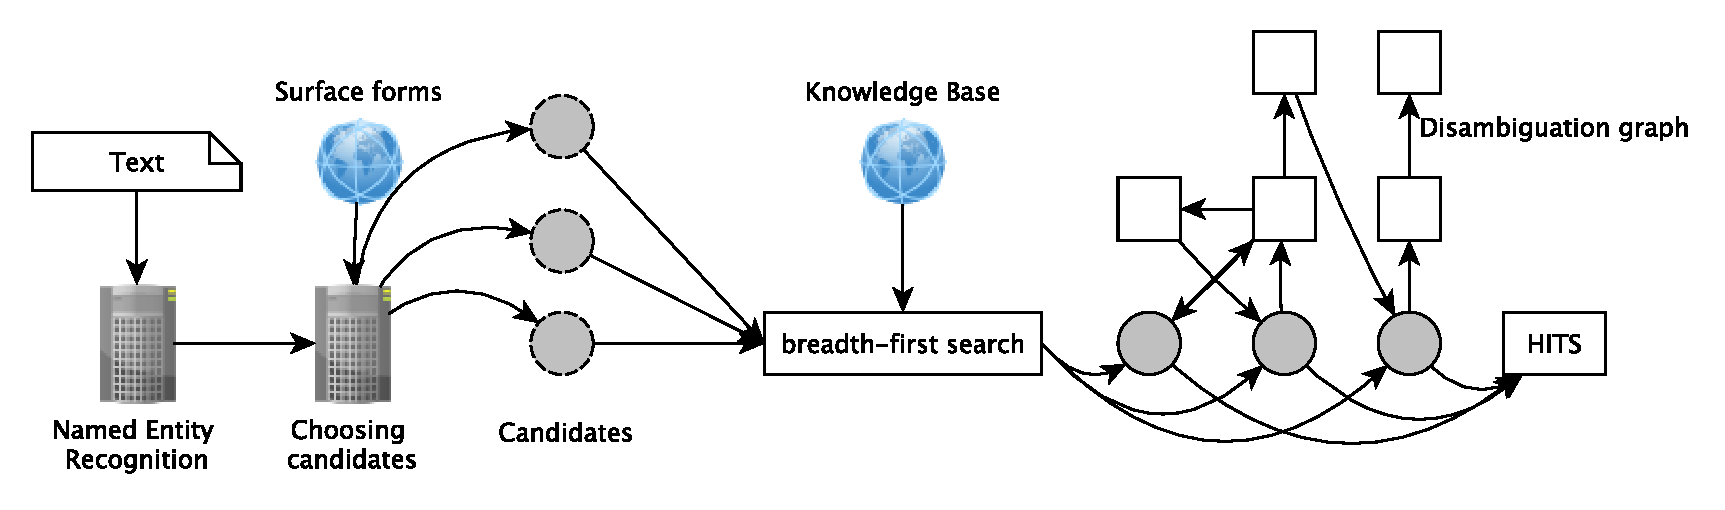
\includegraphics[width=\linewidth]{part_02/unstructured_annotation/fig/overview.pdf}
\caption{Architecture of AGDISTIS.}
\label{fig:overview_agdistis}
\end{figure*}

Our approach to \ac{NED} thus consists of three main phases as depicted in Figure~\ref{fig:overview_agdistis}.
Given an input text $T$ and a named entity recognition function, e.g., FOX~\cite{FOX}, we begin by retrieving all named entities from the input text.
Thereafter, we aim to detect candidates for each of the detected named entities.
To this end, we apply several heuristics and make use of known surface forms~\cite{spotlight} for resources from the underlying \ac{KB}.
The set of candidates generated by the first step is used to generate a disambiguation graph. 
Here, we rely on a graph search algorithm which retrieves context information from the underlying \ac{KB}. 
Finally, we employ the  \ac{HITS} algorithm to the context graph to find authoritative candidates for the discovered named entities.
We assume that the resources with the highest authority values represent the correct candidates.
All algorithms in AGDISTIS have a polynomial time complexity, leading to AGDISTIS also being polynomial in time complexity.
Choosing candidates relates to the notion of $\phi$ while calculating the authority values confers to $\psi$.
In the following, we present each of the steps of AGDISTIS in more detail.

\subsection{Candidate Detection}\label{choosing}

In order to find the correct disambiguation for a certain set of named entities, we first need to detect candidate resources in the \ac{KB}. 
We begin by creating an index comprising all labels of each resource.
Our approach can be configured to use any set of properties as labeling properties, e.g., those in Ell et al.~\cite{ELL+11}. 
For our experiments, we only considered \texttt{rdfs:label} as labeling property.
In addition, our approach can make use of known \emph{surface forms} for each of the resources in case such knowledge is available~\cite{spotlight}.
These are simply strings that are used on the Web to refer to given resources.
Surface forms are simply added to the set of available labels for each resource, cf.\ Section~\ref{eval}.
In this paper, we do not consider abbreviations although these could be easily regarded by adding further labels into the \ac{KB}, e.g., via WordNet~\cite{wordnet}.
%\todo[inline]{remove the above sentence because of missing scientific eval?}

Next to searching the index, we apply a \emph{string normalization} approach and an \emph{expansion policy} to the input text:

The string normalization is based on eliminating plural and genitive forms, removing common affixes such as postfixes for enterprise labels and ignoring candidates with time information (years, dates, etc.) within their label.
For example, the genitive \texttt{New York's} is transformed into \texttt{New York}, the postfix of \texttt{Microsoft Ltd.} is reduced to \texttt{Microsoft} and the time information of \texttt{London 2013} is ignored.

Our \emph{expansion policy} is a time-efficient approach to coreference resolution, which plays a central role when dealing with text from the Web, cf.~Singh et al.~\cite{singh}. 
In web and news documents, named entities are commonly mentioned in their full length the first time they appear, while the subsequent mentions only consist of a substring of the original mention due to the brevity of most news data.
For example, a text mentioning Barack Obama's arrival in Washington D.C. will commonly contain \texttt{Barack Obama} in the first mention of the entity and use strings such as \texttt{Obama} or \texttt{Barack} later in the same text, see Example~\ref{ex:obama}.
We implement this insight by mapping each named entity label, e.g., \texttt{Obama}, which is a substring of another named entity label that was recognized previously, e.g., \texttt{Barack Obama}, to the same resource, i.e., \texttt{dbr:Barack\_Obama}.
If there are several possible expansions, we choose the shortest as a fast coreference resolution heuristic for web documents.
Without the expansion policy AGDISTIS suffers from a loss of accuracy of $\approx4\%$.




%This is simply due to humans readers being able to carry out a co-reference analysis on the fly.

%Internally, AGDISTIS begins its disambiguation by employing the string expansion policy\footnoterecall{myfootnote}.
%Our policy stores all named entity strings in order of their string length.
%If we recognize an entity string matching a part of an already processed entity, we expand the current string to the one stored earlier.
%This assumes both named entities mention the same instance.


%After expanding named entities we harness additional well-known linguistic heuristics.
%Named entities occur often in plural and genitive forms,\,i.e., AGDISTIS tries to identify and stem those words. 
%For example, the genitive form of the named entity \texttt{Obama's} is transformed into \texttt{Obama}.
%Additionally, AGDISTIS reduces plural strings such as \texttt{Obamas} to the singular form \texttt{Obama}.
%Another heuristic is to remove common affixes. 
%For example, we remove affixes which stands for the form of enterprises, such as \emph{corp} and \emph{ltd},\,e.g., \texttt{Hanover Insurance Corp.} is shrunk to \texttt{Hanover Insurance} in order to find candidates for this string in the \ac{KB}.  	
%We observed a significant data quality problem considering affixes in the examined knowledge bases.
%AGDISTIS also eliminates candidates with years and dates within the label so as to be time-independent and to prune the search space.
%One key advantage of Linked Data is the possibility to retrieve a class for each instance in a \ac{KB}.
%By using entity types (obtained via the \texttt{\ac{RDF}:type} property), a domain fitting of possible candidates is implemented, narrowing the search space. 
\begin{table}[htb!]
\centering
 \begin{tabular}{lll}
	\toprule
\textbf{} & \textbf{Class} & \texttt{\textbf{rdf:type}}\\
\midrule
DBpedia & Person & \texttt{dbo:Person}, \texttt{foaf:Person}\\
DBpedia & Organization & \texttt{dbo:Organization}, \texttt{dbo:WrittenWork} (e.g., Journals) \\
DBpedia & Place & \texttt{dbo:Place}, \texttt{yago:YagoGeoEntity} \\
\midrule
YAGO2 & Person & \texttt{yago:yagoLegalActor}  \\
YAGO2 & Organization & \texttt{yago:yagoLegalActor}, \\
  &   &  \texttt{yago:wordnet\_exchange\_111409538} (e.g., NASDAQ) \\
YAGO2 & Place & \texttt{yago:YagoGeoEntity} \\
\bottomrule

 \end{tabular}
  \caption{DBpedia  and YAGO2 classes used for disambiguation classes.}
  \label{tab:tableOfClasses}
 \end{table}
 
 
Additionally, AGDISTIS can be configured to fit named entities to certain domains to narrow the search space.
Since our goal is to disambiguate persons, organizations and places, AGDISTIS only allows candidates of the types mentioned in Table~\ref{tab:tableOfClasses} when run on DBpedia and YAGO2.
Adding general types will increase the number of candidates and thus decrease the performance.
Obviously, these classes can be altered by the user as required to fit his purposes. 


\begin{algorithm}[htb!]
\KwData{label of a certain named entity $N_i$, $\sigma$ trigram similarity threshold}
\KwResult{$C$ candidates found}
$C \longleftarrow \emptyset$\;
{\bf label } $\longleftarrow$ {\bf normalize(label)}\;
{\bf label } $\longleftarrow$ {\bf expand(label)}\;
$ \displaystyle \bar C \longleftarrow$ {\bf searchIndex(label)}\;
\For{{\bf c} $\in \bar C$}{
    \If{$\neg${\bf c .matches([0-9]$^+$)}}{
        %\If{$\neg${\bf isDisambiguationSite(c})} {
         %          {\bf continue}\;
          %      }
        \If{{\bf trigramSimilarity(c, label)}$ \geq \sigma$}{
            \If{{\bf fitDomain(c)}} {
                $C \longleftarrow C \cup $ {\bf c}\;
            }
        }
        % The same as the two ifs above but with a continue
        %\If{{\bf trigramSimilarity(c, label)}$ < \sigma$} {
        %           {\bf continue}\;
        %        }
        %% {\bf c} $\longleftarrow$ {\bf redirect(c)}\;
        %\If{{\bf fitDomain(c)}} {
        %     $C \longleftarrow C \cup $ {\bf c}\;
        %        } 
        %}
    }
}
\caption{Searching candidates for a label.}
\label{findingCandidates}
\end{algorithm}



The resulting candidate detection approach is explicated in Algorithm~\ref{findingCandidates}.
%If a \ac{KB} provides redirect and disambiguation URLs, AGDISTIS can benefit from them.
%\todo[inline]{added  a virtual function in this algorithm 1 for the grammatical functions}
%For example, it is straightforward to use \texttt{dbo:wikiPageRedirects} for identifying multiple labels for one instance. 
%Of course AGDISTIS ignores disambiguation entities as they would not help accomplishing the disambiguation goal and finding $\mu^{+}$. 
%\todo[inline]{AN:What's a disambiguation entity?}
In its final step, our system compares the heuristically obtained label with the label extracted from the \ac{KB} by using \emph{trigram similarity} which is an n-gram similarity with $n=3$. 

\subsection{Computation of Optimal Assignment}

Given a set of candidate nodes, we begin the computation of the optimal assignment by constructing a disambiguation graph $G_d$ with search depth $d$.
To this end, we regard the input \ac{KB} as a directed graph $G_K = (V, E)$ where the vertices $V$ are resources of $K$, the edges $E$ are properties of $K$ and $x,y\in V, (x,y) \in E \Leftrightarrow \exists p : (x, p, y) \mbox{ is an \ac{RDF} triple in }K$.
Given the set of candidates $C$, we begin by building an initial graph $G_0 = (V_0, E_0)$ where $V_0$ is the set of all resources in $C$ and $E_0=\emptyset$. %$\forall (x, y) \in V_0^2, (x, y) \in E_0 \Rightarrow (x, y) \in K$.
Starting with $G_0$ we extend the graph in a breadth-first search manner.
Therefore, we define the extension of a graph $G_i = (V_i, E_i)$ to a graph as follows:
\begin{equation}
\rho(G_i) = G_{i+1} = (V_{i+1}, E_{i+1}) \textnormal{ with } i=0, \ldots, d
\end{equation}
\begin{equation}
V_{i+1} = V_i \cup \{y : \exists x \in V_i \wedge (x, y) \in E\}
\end{equation}
\begin{equation}
E_{i+1} = \{(x,y) \in E: x, y \in V_{i+1}\}
\end{equation}
We iterate the $\rho$ operator $d$ times on the input graph $G_0$ to compute the initial disambiguation graph $G_d$.

%Empirically, we see no effect on the \mbox{F-measure} when using spread activation instead~\cite{Kleb11WIMS} (despite the obvious extra computational costs).

After constructing the disambiguation graph $G_d$, we need to identify the correct candidate node for a given named entity.
Using the graph-based  \ac{HITS} algorithm, we calculate authoritative values $x_a,y_a$ and hub values $x_h,y_h$ for all $x,y\in V_d$.
We initialize the authoritative and hub values $x_a$ respectively $x_h$:
\begin{equation}
\forall x \in V_d, x_a=x_h=\frac{1}{|V_d|}  .
\end{equation}
Afterwards, we iterate the equations $k$ times as follows: 
\begin{equation}
x_a = \sum_{(y,x)\in E_d} y_h
\end{equation}
\begin{equation}
y_h = \sum_{(y,x)\in E_d} x_a 
\end{equation}
We choose $k$ according to Kleinberg~\cite{HITS}, i.e., 20 iterations, which suffice to achieve convergence in general. %d authoritative values $x_a$ and hub values $y_h$.
Afterwards, we identify the most authoritative candidate $C_{ij}$ among the set of candidates $C_i$ as correct disambiguation for a given named entity $N_i$. %sort the nodes according to their authoritative values in descending order. 
%The first candidate for a certain named entity is assumed to be the correct disambiguation.
When using DBpedia as \ac{KB} and $C_{ij}$ is a redirect AGDISTIS uses the target resource. %follows redirecting resources transitively. %can use redirections to di%maps redirecting resources to their most authoritative redirection.
AGDISTIS' whole procedure is presented in Algorithm~\ref{algooverview}.
As can be seen, we calculate $\mu^{+}$ solely by using polynomial time complex algorithms.
%Thus, we observe on average better run time performance than the state-of-the-art approach AIDA, see Section~\ref{results}. % Appendix Figure 3).
%\todo[inline]{Again, we have no Appendix here}
\begin{algorithm}[htb!]
\KwData{$N=\{N_1,N_2\dots N_n\}$ named entities, $\sigma$ trigram similarity threshold, $d$ depth, $k$ number of iterations}
\KwResult{$C = \{C_1,C_2\dots C_n\}$ identified candidates for named entities}
$E \longleftarrow \emptyset$\;
$V \longleftarrow${\bf insertCandidates($N, \sigma$)}\;
$G \longleftarrow (V,E)$\;
$G \longleftarrow${\bf breadthFirstSearch($G,d$)}\;
{\bf  HITS($G(V,E), k$)}\;
{\bf sortAccordingToAuthorityValue(V)}\;
\For{$N_i \in N$} {
    \For{$v \in V$}{
        \If{$v$ {\bf is a candidate for} $N_i$  }{
              {\bf store($N_i$,$v$)}\;
              {\bf break}\;
          }
     }
}
\caption{Disambiguation Algorithm based on \ac{HITS} and Linked Data.}
\label{algooverview}
\end{algorithm}


For our example, the graph depicted in Figure~\ref{fig:example} shows an excerpt of the input graph for the  \ac{HITS} disambiguation algorithm when relying on DBpedia as \ac{KB}. 
%Depending on the used \ac{KB} properties may exist that lead to bi-directional edges (e.g., \texttt{sex} vs. \texttt{fatherOf}).
The results can be seen in Table~\ref{tab:example}. 
%Obviously a disambiguation towards the correct named entity URIs is possible.
%\todo{what happens if the \ac{KB} does not contain the correct entity, does the algorithm answer null, but is encompanied with closed world assumption, we know all entities we annotated}
%Since we assume a closed-world scenario our algorithm supposes every entity to be in the \ac{KB}.

\begin{figure}[htb!]
	\begin{minipage}[b]{0.57\textwidth} 
       % \begin{figure}
         \centering
        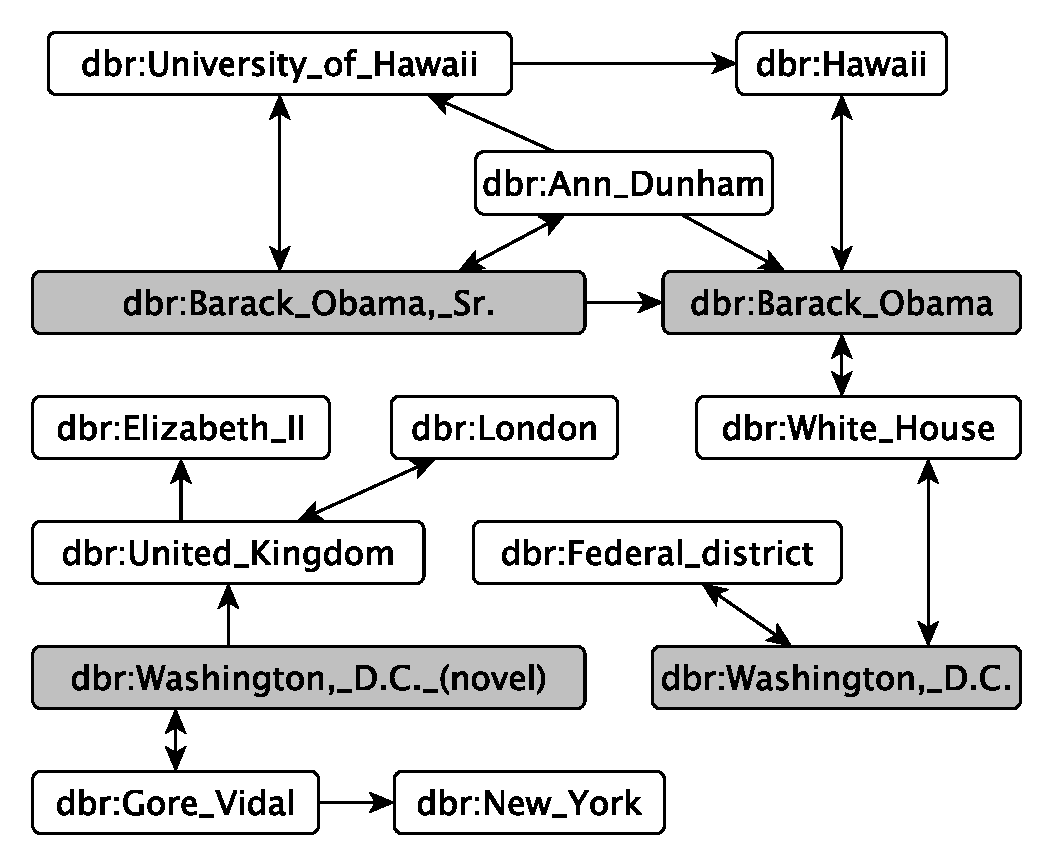
\includegraphics[width=\linewidth]{part_02/unstructured_annotation/fig/exampleGraph.pdf}
        \caption{One possible graph for the example sentence, with candidate nodes in grey.}
        \label{fig:example}
      %  \end{figure}
    \end{minipage}
	\hfill
	\begin{minipage}[b]{0.42\textwidth}
       % \begin{table}
        \centering
        
        \resizebox{\textwidth}{!}{ 
        \begin{tabular}{lc}
            \toprule
            \textbf{Node}  & \textbf{$x_a$} \\
            \midrule
            \texttt{dbr:Barack\_Obama} & 0.273 \\
            \texttt{dbr:Barack\_Obama,\_Sr.} & 0.089 \\
            \texttt{dbr:Washington,\_D.C.} & 0.093 \\
            \texttt{dbr:Washington,\_D.C.\_(novel)} & 0.000 \\
            \bottomrule
        \end{tabular}}
        \captionof{table}{Nodes and their according authority weights for the example graph.}
        \label{tab:example}
        \vspace{1.8cm}
       % \end{table}
	\end{minipage}
\end{figure}

%%Idea of the extension
%The most words of a document given to AGDISTIS are no named entities.
%Therefore, AGDISTIS does not use them in its workflow.
%Because a human reader would use all words for the disambiguation task we thought of an extension of AGDISTIS which uses the additional words, too.
%With these words AGDISTIS would be able to recognize the topical structure of the document and could use these information for the disambiguation task.
%Therefore, we added an extension which uses topic modeling to consider the topical structure.

%%what is topic modeling
%\emph{Probabilistic topic modeling} is a research area that aims to discover thematic information inside large corpora \cite{Blei:2012:PTM:2133806.2133826}.
%It is based on the definition of generative models that describe the creation of documents and how this process is influenced by latent topics.
%A very famous model is \emph{Latent Dirichlet Allocation (LDA)} \cite{Blei:2003:LDA:944919.944937}.
%Its generative process is based on a set of Topics $T$ and a vocabulary $V$.
%For the creation of a document $d$ the distribution of the topics inside this document $\theta_d=\left \{P(t_0|d), \ldots, P(t_{|T|}|d) \right \}$ is sampled.
%After that for every $i$th-word the id $z_i$ of a topic $t_{z_i}$ is sampled from $\theta_d$.
%Every topic $t \in T$ has a vector $\phi_{t}=\left \{P(w_0|t), \ldots, P(w_{|V|}|t) \right \}$ which defines the probabilities of all words under this topic.
%After $z_i$ has been sampled the word is sampled from $\phi_{t_{z_i}}$ \cite{Blei:2012:PTM:2133806.2133826}.
%Figure TODO shows the graphical model of LDA.
%The figure contains $\alpha$ and $\beta$ which are hyperparameter for the $\theta$ and $\phi$ distributions respectively.
%\todo[inline]{Add graphic with plate notation}

%In figure TODO all variables are white except the word $w$ which is shaded.
%This means that $w$ is the only variable which can be observed and all other variables are latent.
%So starting with the observable words inside of the documents of a corpus the other variables have to be inferenced.
%Because a direct solution of the inference problem is intractable there are several algorithms for approximating the variables \cite{Blei:2012:PTM:2133806.2133826}.
%For our experiments we used Mallet which contains an implementation of Gibbs-Sampling \cite{McCallumMALLET,griffiths2004finding}.

%\todo[inline]{* definition \newline* LDA \newline* generative model \newline* how do we use it \newline* where does the model come from\newline * \textbf{what are we doing with the model and the texts}}

\section{Evaluation}
\label{sec:eval}

This section is divided into four parts. 
First, we explain the experimental setup, i.e., which measures we chose for evaluation.
Then, we describe the datasets underlying the experiments. 
Afterwards, the evaluation results are analyzed and conclusion are drawn. 
We devote a single subsection to the generation and evaluation of the Chinese benchmark since it is the first benchmark w.r.t. Chinese \ac{NED}.

\subsection{Experimental Setup}
\label{eval}
The aim of our evaluation is two-fold.
First, we want  to determine the F-measure achieved by our approach on different datasets.
Several definitions of F-measure have been used in previous work on \ac{NED}.
Cornolti et al.~\cite{cornolti} define the micro F-measure (F1) w.r.t. a strong annotation match, i.e., a binary relation, and the possibility of assigning null to an entity.
This micro F-measure, which we use throughout our evaluation, aggregates all true/false positives/negatives over all documents.
Thus, it accounts for larger contexts in documents with more annotations, cf. Cornolti et al.~\cite{cornolti, GERBIL}.
For a more detailed explanation of evaluation measures please cf. Chapter~\ref{cha:gerbil}.

%In addition to the traditional definition of false and true positives and negatives when given a reference mapping between strings and resources, 
%we regarded the assignment of a resource to a string as a \emph{false positive} if no resource from the \ac{KB} mapped with the string or if the string was assigned to the wrong resource.
%Furthermore, the assignment of a resource was considered a \emph{false negative} if the approach returned that no resource mapped the string although there was a resource in the \ac{KB} that did.

Second, we want to know how AGDISTIS performs in comparison to other state-of-the-art \ac{NED} approaches. 
Thus, we compare AGDISTIS with TagMe 2~\cite{TagMe2}, the best approach according to Cornolti et al.~\cite{cornolti} as well as with AIDA~\cite{AIDA} and DBpedia Spotlight~\cite{spotlight} because they are well-known in the Linked Data community. 
AGDISTIS is designed to be agnostic of the underlying \ac{KB}.
Thus, we use the German and English DBpedia \ac{KB} as well as the English YAGO 2 \ac{KB}. %\footnote{Results using other Linked Data \ac{KB}s can be found at the project homepage.}

Within our experiments, we ran AGDISTIS with the following parameter settings: 
the threshold $\sigma$ for the trigram similarity was varied between 0 and 1 in steps of 0.01. 
Additionally, we evaluated our approach with $d=1,2,3$ to measure the influence of the size of the disambiguation graph on AGDISTIS' F-measure.
%In this paper we use accuracy to measure directly the percentage of correctly disambiguated entities instead of the also common precision and recall values.
%We also ran the experiments without using the graph,\,i.e., only applying all heuristics and trigram similarity.
%We did not consider abbreviations and thus ignored labels shorter than three characters.
For our experiments, we fitted AGDISTIS to the domain of named entity recognition and only allow candidates of the types mentioned in Table~\ref{tab:tableOfClasses}.
%While, we were not able to identify all entities in all datasets resulting in a worse F1-measure than possible. 
%Moreover, %a closed world was assumed,\,i.e., entities that were not in the \ac{KB} were not considered in our evaluation.
%We used YAGO2 (English) as well as the German and the English versions of DBpedia as underlying \ac{KB}s for AGDISTIS.
%While the results reported in this paper only use the English versions of DBpedia 3.9 as underlying \ac{KB}, we also evaluated AGDISTIS on YAGO2 and the German version of DBpedia 389. 
We report more details on the evaluation setup as well as complete results at the project homepage.
%\todo[inline]{Micha: But this would be possible now, wouldn't it?}

%Note that for most entities from DBpedia a direct matching to YAGO2 entities can easily be applied. 
%Web news texts are a common input for disambiguation systems~\cite{Cucerzan07,fox}.
%Third, we wanted to measure how time-efficient AGDISTIS is. 
%To this end, we compared its runtime with that of AIDA.
%We were not able to compare AGDISTIS' runtime with that of Spotlight due to Spotlight's high RAM requirements.
%\todo[inline]{not RAM but webservice}
%Finally, we analyzed the impact of removing certain properties on the \mbox{F-measure}.
%We carried out all our experiments on the following four datasets:\newline
%: (1) a subset of the well-known Reuters-21578 dataset, (2) RSS feeds extracted from 1,500 sources, (3) a German news corpus extracted from \url{news.de} and (4) the original AIDA dataset from~\cite{AIDA}, which contains 1,393 annotated news reports.
%%For each corpus, we generated a spell-corrected version of annotations. % assuming that a used disambiguation system would incorporate such a module.
%%\todo[inline]{Discuss whether pointing to a spell corrected version can be left out}
%We annotated the first dataset manually while the others were already annotated and used in previous works.
%%Some documents comprise only little or no annotations to account for the sparsity and shortness of WND. 
%%Furthermore, only the in Table~\ref{tab:tableOfClasses} mentioned resource classes were annotated.
%%\todo{explain why reagan and not reagan area is annotated}
%\footnote{To preserve the anonimity of the authors, we refrained from adding a link to the page for downloading the data. A link to this page will be added in the final version of the paper.}
%The test corpora can be downloaded from \url{https://github.com/XYZ}.%https://github.com/AKSW/AGDISTIS}.

\subsection{Datasets}
Noisy and incorrect datasets can affect the performance of \ac{NED} approaches which can be prevented by using well-known datasets.
We carried out our evaluation on the following nine different, publicly available datasets, which consists of the three corpora from the benchmark dataset \textbf{N3}~\cite{n3} (see chapter~\ref{cha:N3}), the original AIDA evaluation corpus\footnote{\url{https://www.mpi-inf.mpg.de/departments/databases-and-information-systems/research/yago-naga/aida/downloads/}} and four of the five datasets from the Cornolti et al.~\cite{cornolti} benchmark. Furthermore, we used the multilingual QALD 4 dataset for the evaluation of the Chinese version of AGDISTIS.

\begin{enumerate}
\item \textbf{Reuters-21578 Dataset.}
The first of the N3 datasets comprises 145 news articles randomly sampled from the Reuters-21578 news articles dataset.
Two domain experts determined the correct URI for each named entity using an online annotation tool reaching a initial voter agreement of $74\%$.
%Although we have no agreement values for AIDA, we consider 74\% as an upper bound for human capability for \ac{NED} tasks.
%In comparison, DBpedia Spotlight achieved a \emph{Fleiss' Kappa} maximum of 0.67~\cite{spotlight} during creation of their dataset.
%\todo{compare the interrater agreement with the one of AIDA: AIDA didn't mention agreement rate, AIDA used 2 students and resolved in case of conflict}
In cases where the judges did not agree initially, they concerted each other and reached an agreement.
This initial agreement rate hints towards the difficulty of the disambiguation task.
The corpus does not annotate ticker symbols of companies, e.g., \textit{GOOG} for Google Inc., abbreviations and job descriptions because those are always preceded by the full company name respectively a person's name.
%Since AGDISTIS relies on a closed-world assumption, 
%Finally, we generated a default URI for instances which could not be identified within a 5-minute Web search while annotating. 

\item \textbf{\url{news.de} Dataset.}
This real-world dataset is the second of the N3 datasets and was collected from 2009 to 2011 from the German web news portal \url{news.de} ensuring that each message contains the German word \emph{Golf}.
This word is a homonym that can semantically mean a geographical gulf, a car model or the sport discipline.
This dataset contains 53 texts comprising over 600 named entities that were annotated manually by a domain expert.
Although some meanings of Golf are not within the class range of our evaluation, they are kept for evaluation purposes.

\item \textbf{RSS-500 Dataset.}
This corpus has been published in Gerber et al.~\cite{GER+13} and is the third of the of the N3 datasets.
It consists of data scrapped from 1,457 RSS feeds. % as compiled in Goldhahn~\shortcite{GOLDHAHN12.327}.
The list includes all major worldwide newspapers and a wide range of topics,\,e.g., \emph{World}, \emph{U.S.}, \emph{Business}, \emph{Science} etc.
This list was crawled for 76 hours, which resulted in a corpus of about 11.7 million sentences.
A subset of this corpus has been created by randomly selecting $1\%$ of the contained sentences.
Finally, domain experts annotated 500 sentences manually. 
Further information about the corpora and the datasets themselves can be found on the project homepage.\footnote{\url{http://aksw.org/Projects/N3NERNEDNIF.html}}
%These sentences were a subset of those which contained a natural language representation of a formal relation, like ``\ldots, who was born in\ldots '' for \texttt{dpo:birthPlace} (see ~\cite{conf/ekaw/GerberN12}), that occurred more then 5 times in the 1\% corpus. %with DBpedia URIs or created new URIs in case the mentioned entity was not contained in DBpedia.

\item \textbf{AIDA-YAGO2 Dataset.}
This is the original dataset that was used while evaluating AIDA~\cite{AIDA}, stemming from the CoNLL 2003 shared task~\cite{conll2003} and comprising 1,393 news articles which were annotated manually. % with 34,956 entity mentions.
%Possible conflicts resulting from two annotators were resolved.
Two students annotated each entity resolving conflicts by the authors of AIDA. 
%AIDA-YAGO2 has 34,956 entity mentions from the YAGO2 ontology.%\footnote{\url{http://www.mpi-inf.mpg.de/yago-naga/yago/}}.

\item  \textbf{AIDA/CoNLL-TestB} This dataset originates from the Cornolti et al. benchmarks~\cite{cornolti} and originates from the evaluation of AIDA~\cite{AIDA}. 
As mentioned above, this dataset was derived from the CoNLL 2003 shared task. %~\cite{conll2003} and comprises 1,393 news articles which were annotated manually. 
Cornolti et al.'s benchmark consists only of the second test part comprising 231 documents with 19.4 entities per document on average.

\item \textbf{AQUAINT} In this dataset, only the first mention of an entity is annotated. The corpus consists of 50 documents which are on average longer than the AIDA/CO-NLL-TestB documents. Each document contains 14.5 annotated elements on average
The documents originate from different news services, e.g. Associated Press and have been annotated using voter agreement.
The dataset was created by Milne et al.~\cite{milne2008learning}.

\item \textbf{IITB} The IITB corpus comprises 103 manually annotated documents. Each document contains 109.1 entities on average.
This dataset displays the highest entity/document-density of all corpora.
This corpus has been presented by Kulkarni et al.~\cite{kulkarni2009collective} in 2009.

\item \textbf{MSNBC} This corpus contains 20 news documents with 32.9 entities per document. This corpus was presented in 2007 by Cucerzan et al.~\cite{Cucerzan07}.

\item \textbf{QALD 4} This dataset is a first try to adopt the multilingual benchmark provided in Question Answering over Linked Data (\ac{QALD}) 4~\cite{qald4} for \ac{NED}. Unfortunately, the Chinese language is not supported. Therefore, we extended the QALD 4 benchmark by translating the English questions to Chinese and annotated the named entity links manually. The links in the given SPARQL queries for the questions are assumed to be the correct links for the English entities, which are adapted to the Chinese links by hand. It results in 200 Chinese questions in the training data and 50 ones in the test data, with an average of 0.9 named entities links per question. \footnote{The Chinese benchmark is available at \url{https://github.com/wencanluo/DBpediaQA/tree/master/benchmark/qald4}.}

\end{enumerate}

We did not use the \textbf{Meij} dataset from Cornolti et al. since it comprises only tweets from twitter with 1.6 entities per document. The number of entities available in the datasets is shown in Table~\ref{tab:data}.
%\todo{leave the computer stuff out?}
All experiments were carried out on a MacBook Pro with a 2.7 GHz Intel Core i7 processor and 4 GB 1333 MHz DDR3 RAM using Mac OS 10.7. 


\begin{table*}[htb!]
\centering

\resizebox{\textwidth}{!}{ 
\begin{tabular}{lcrrrc}
\toprule
\textbf{Corpus} & \textbf{Language} & \textbf{\#Doc.} & \textbf{\#Ent.} & \textbf{Ent./Doc.} & \textbf{Annotation}\\
\midrule
AIDA/CoNLL-TestB  & English & 231 & 4458 &19.40& voter agreement\\
AQUAINT & English & 50 & 727 & 14.50 &voter agreement\\
IITB & English & 103 & 11,245 & 109.01 &domain expert\\
MSNBC & English & 20 & 658 &31.90 &domain expert\\
Reuters-21578  & English & 145 & 769 &5.30 &voter agreement\\
RSS 500 & English & 500 & 1,000 & 2.00&domain expert \\
\url{news.de} & German & 53 & 627 & 11.83 &domain expert\\
AIDA-YAGO2 & English & 1,393 & 34,956 &25.07 &voter agreement\\
QALD 4 & Chinese & 250 & 196 & 0.78 &domain expert\\

\bottomrule
\end{tabular}
}
\caption{Test corpora specification including the number of documents (\#Doc.) and the number of named entities (\#Ent.) per dataset}
\label{tab:data}

\end{table*}


%\begin{figure*}[tb!]
%    \centering
%        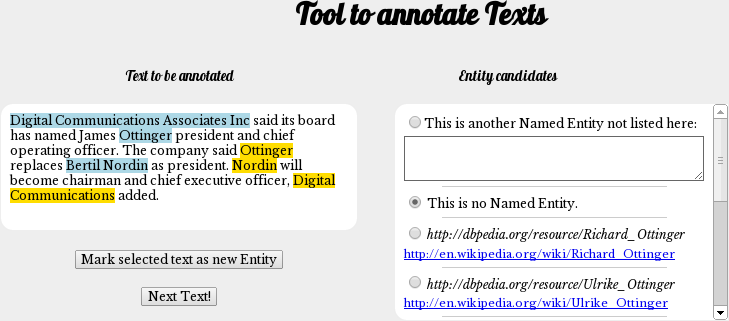
\includegraphics[width=\linewidth]{fig/qrtoolnew.png}
%    \caption{GUI of our annotation tool.}
%    \label{fig:qrtool}
%\end{figure*}

\subsection{Evaluation}
\label{results}



First, we evaluate AGDISTIS against AIDA and DBpedia Spotlight on three different knowledge bases using N3 corpora and the AIDA-YAGO2 corpus. 

AGDISTIS performs best on the \url{news.de} corpus, achieving a maximal 0.87 F\-measure for $\sigma = 0.71$ and $d = 2$ (see Table~\ref{tab:evalold}).
Our approach also outperforms the state of the art on Reuters-21578 corpus, see Figure~\ref{fig:reuters}, where it reaches 0.78 \mbox{F-measure} for $\sigma = 0.87$ and $d = 2$.
Considering the AIDA-YAGO2 dataset AGDISTIS achieves an \mbox{F-measure} of 0.73 for $\sigma = 0.89$ and $d = 2$.
%In combination with the results on RSS-500, 
Our results suggest that $d=2, \sigma=0.82$ and using DBpedia as \ac{KB} are a good setting for AGDISTIS and suffice to perform well. %The iteration of $\sigma$ between $0.7$ and $0.9$ can lead to an improvement of up to $6\%$ \mbox{F-measure}.
In the only case where $\sigma=0.29$ leads to better results (Reuters-21578 corpus), the setting $0.7<\sigma<0.9$ is only outperformed by 0.03 F-measure using YAGO as \ac{KB} for AGDISTIS.


\begin{table*}[htb!]
\centering

\resizebox{\textwidth}{!}{ 
\begin{tabular}{c ccc ccc c c}
\toprule
\textbf{Corpus}  & \multicolumn{6}{c}{\textbf{AGDISTIS}}	& \textbf{AIDA} & \textbf{Spotlight}\\\midrule
\textbf{$K$}& \multicolumn{3}{c}{{DBpedia}}& \multicolumn{3}{c}{{YAGO2}}	& {YAGO2} & {DBpedia}\\\midrule
				& \mbox{F-measure} 		& $\quad \sigma \quad $ & $\quad d \quad $ 	& \mbox{F-measure} & $\quad \sigma \quad $ & $\quad d \quad $ & \mbox{F-measure}  & \mbox{F-measure}\\
\cmidrule(r){2-4}  \cmidrule(r){5-7} \cmidrule{8-8} \cmidrule{9-9}
Reuters-21578	&  	\textbf{0.78}	&  			0.87		&  		2		& 	0.60	&  0.29		&  	3	&  	0.62		& 	0.56	\\
RSS-500 		&  	\textbf{0.75}	&  			0.76		&  		2		& 	0.53	&  0.82		&   2 	&  	0.60		& 	0.56	\\
\url{news.de} 	&  	\textbf{0.87}	&  			0.71		&  		2		& 	---		&   ---		&  ----	&  	----		& 	0.84	\\
AIDA-YAGO2	   	&  		0.73		&  			0.89		&  		2		& 	0.58	&  0.76		&   2 	&\textbf{0.83}	& 	0.57	\\
\bottomrule
\end{tabular}}
\caption{Evaluation of AGDISTIS against AIDA and DBpedia Spotlight. Bold indicates best \mbox{F-measure}.} \label{tab:evalold} 
\end{table*}
\begin{figure}[htb!]\centering
        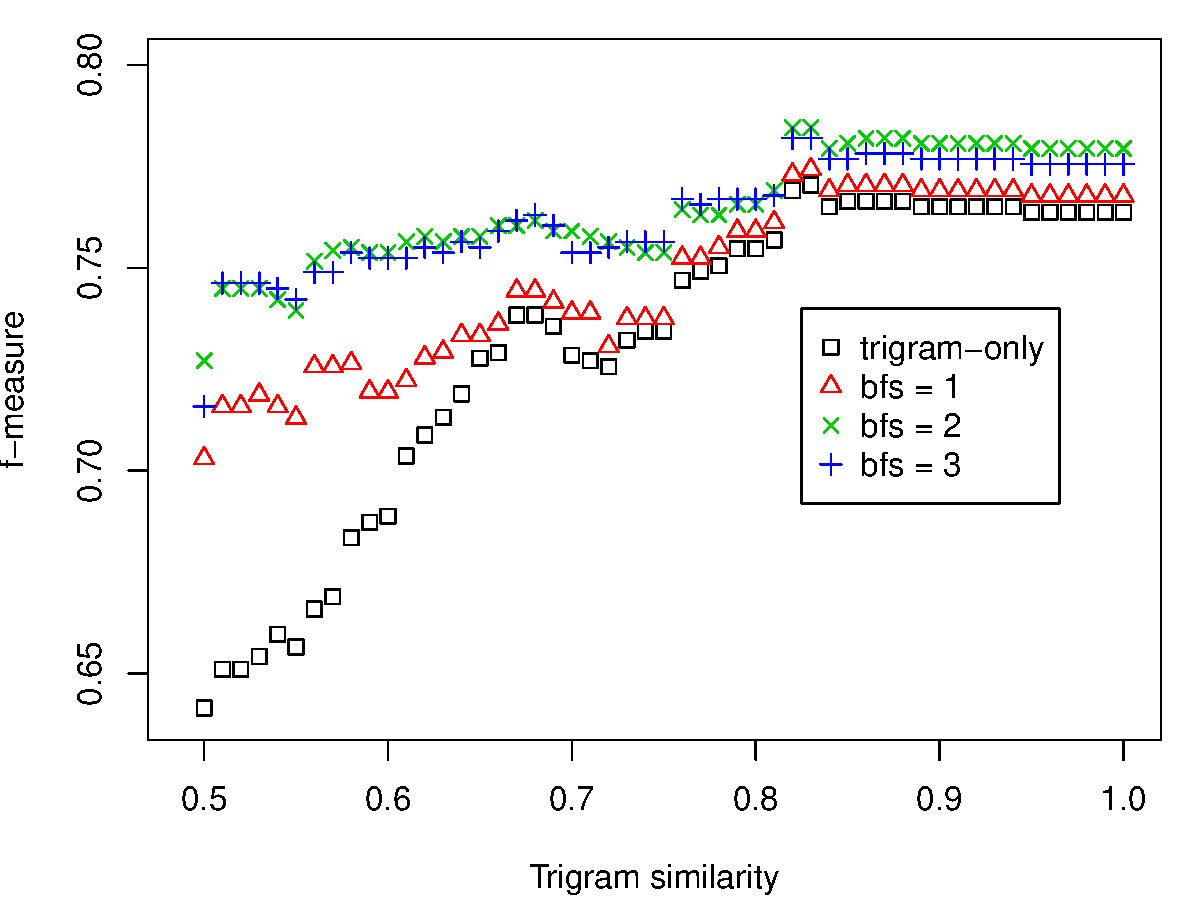
\includegraphics[width=0.9\linewidth]{part_02/unstructured_annotation/fig/reuters.pdf}
        %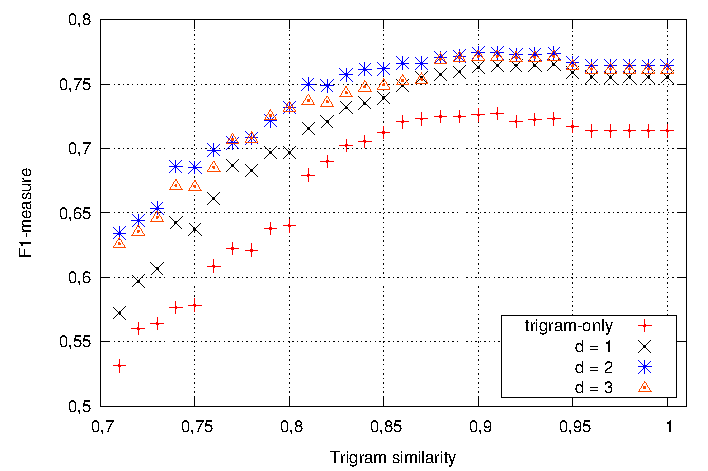
\includegraphics[width=0.9\linewidth]{fig/bfs_depth_diag.pdf}
    \caption{\mbox{F-measure} on the Reuters-21578 corpus using DBpedia as \ac{KB}.}  \label{fig:reuters}
\end{figure}

Second, we compared our approach with TagMe 2 and DBpedia using datasets already implemented in the framework of Cornolti et al.
AGDISTIS has been setup to use a breadth-first search depth $d=2$ and a trigram similarity of $\sigma=0.82$.
All approaches used disambiguate w.r.t. the English DBpedia.
%TagMe 2 and DBpedia Spotlight are easily to test via web services while AIDA needs to be installed locally and run on a large machine. 
AIDA was ommitted from this evaluation because it has been shown to be outperformed by TagMe 2 in~\cite{cornolti} on the datasets we consider. 

AGDISTIS achieves \mbox{F-measures} between $0.31$ (IITB) and $0.76$ (MSNBC), see Table~\ref{tab:evalnew}.
We outperform the currently best disambiguation framework, TagMe 2, on three out of four datasets by up to $29.5\%$ F-measure. 
Our poor performance on IITB is due to AGDISTIS not yet implementing a paragraph-wise disambiguation policy. 
By now, AGDISTIS performs disambiguation on full documents.
The large number of resources in the IITB documents thus lead to our approach generating very large disambiguation graphs.
The explosion of errors within these graphs results in an overall poor disambiguation.
We will address this drawback in future work by fitting AGDISTIS with a preprocessor able to extract paragraphs from input texts.
The local vector-space model used by Spotlight performs best in this setting. 
\begin{table}[htb!]
    \centering

\begin{tabular}[tb]{@{}lllll@{}}
\toprule
Dataset                            & Approach          & \textbf{F-measure}             & \textbf{Precision} & \textbf{Recall} \\ \midrule
\multirow{3}{*}{\begin{minipage}{0.8in}\textbf{AIDA/CO-NLL-TestB}\end{minipage}} & TagMe 2           & 0.565          & 0.58      & 0.551  \\
                                   & DBpedia Spotlight & 0.341          & 0.308     & 0.384  \\
                                   & AGDISTIS          & \textbf{0.596} & \textbf{0.642}     & \textbf{0.556}  \\ \midrule
\multirow{3}{*}{\textbf{AQUAINT}}  & TagMe 2           & 0.457          & 0.412     & \textbf{0.514}  \\
                                   & DBpedia Spotlight & 0.26           & 0.178     & 0.48   \\
                                   & AGDISTIS          & \textbf{0.547} & \textbf{0.777}     & 0.422  \\\midrule
\multirow{3}{*}{\textbf{IITB}}     & TagMe 2           & 0.408          & 0.416     & 0.4    \\
                                   & DBpedia Spotlight & \textbf{0.46}  & 0.434     & \textbf{0.489}  \\
                                   & AGDISTIS          & 0.31           & \textbf{0.646}     & 0.204  \\\midrule
\multirow{3}{*}{\textbf{MSNBC}}    & TagMe 2           & 0.466          & 0.431     & 0.508  \\
                                   & DBpedia Spotlight & 0.331          & 0.317     & 0.347  \\
                                   & AGDISTIS          & \textbf{0.761} & \textbf{0.796}     & \textbf{0.729}  \\ \bottomrule
\end{tabular}
\caption{Performance of AGDISTIS, DBpedia Spotlight and TagMe 2 on four different datasets using micro F-measure (\textbf{F1}).}
\label{tab:evalnew}
\end{table}
%\todo[inline]{Micha: the part "The iteration of $\sigma$ between $0.7$ and $0.9$ can lead to an improvement of up to $6\%$ \mbox{F-measure}" occurs two times. Remove one of them.}  



Delving deeper into AGDISTIS' results lead to the following insights:
\begin{itemize}
\item Varying the search depth $d$ does not significantly improve \mbox{F-measure} because within the underlying documents there are many similar named entities forming a shallow semantic background. However, using only string similarity measures ($d=0$) results in lower F-measure, see Figure \ref{fig:reuters}. % while the optimum has been found using $d=2$. %, see Figure~(\todo[inline]{here was a reference to a reuters figure}). 
\item The expansion policy can have considerable knock-on effects: Either the first entity and its expansions are disambiguated correctly or the wrong disambiguation of the first entity leads to an avalanche of false results in a loss of $\approx 4\%$ accuracy.
%\todo[inline]{Micha: Why accuracy while you always talk about F-measure?}
\item We observed a significant enhancement of AGDISTIS when adding surface forms to the labels of resources as explained in Section~\ref{choosing}.
Employing additional labels (such as surface forms gathered from Wikipedia) increased the \mbox{F-measure} of AGDISTIS by up to $4\%$. 
\item Using $n=1,2,4$ as n-gram similarity has been proven to perform worse than using trigram similarity,\,i.e., $n=3$.
Our results suggest that $d=2$ while using DBpedia as \ac{KB} is a good setting for AGDISTIS and suffice to perform well. 
The iteration of $\sigma$ between $0.7$ and $0.9$ can lead to an improvement of up to $6\%$ \mbox{F-measure} while $\sigma<0.7$ and $\sigma>0.9$ leads to a loss of F-measure.
\end{itemize}


Overall, our results suggest that $\sigma=0.82$ and $d=2$ is generally usable across datasets and knowledge bases leading to high quality results.
Further results, can be found in the Chapter~\ref{cha:app_agdistis} in the appendix.

%This is done by selecting all resources as candidates that are such that the similarity of at least one of its labels and the 
%The best similarity thresholds $\sigma$ w.r.t. disambiguation \mbox{F-measure} achieved by our approach were determined empirically iterating $\sigma$ between 0 and 1 in steps of 0.01. 
%Setting $\sigma=0.82$ turned out to be the best threshold independent of the analysed dataset.%\footnote{See our project side for further evaluation \url{http://aksw.org/Projects/AGDISTIS}}% (cf. Section~\ref{eval}).
%as shown in Figure~\ref{fig:influenceOfSurfaceForms}.
%This explains the worse results achieved by AGDISTIS when using YAGO2 as \ac{KB}. 

%\begin{figure}[htb!]\centering
%        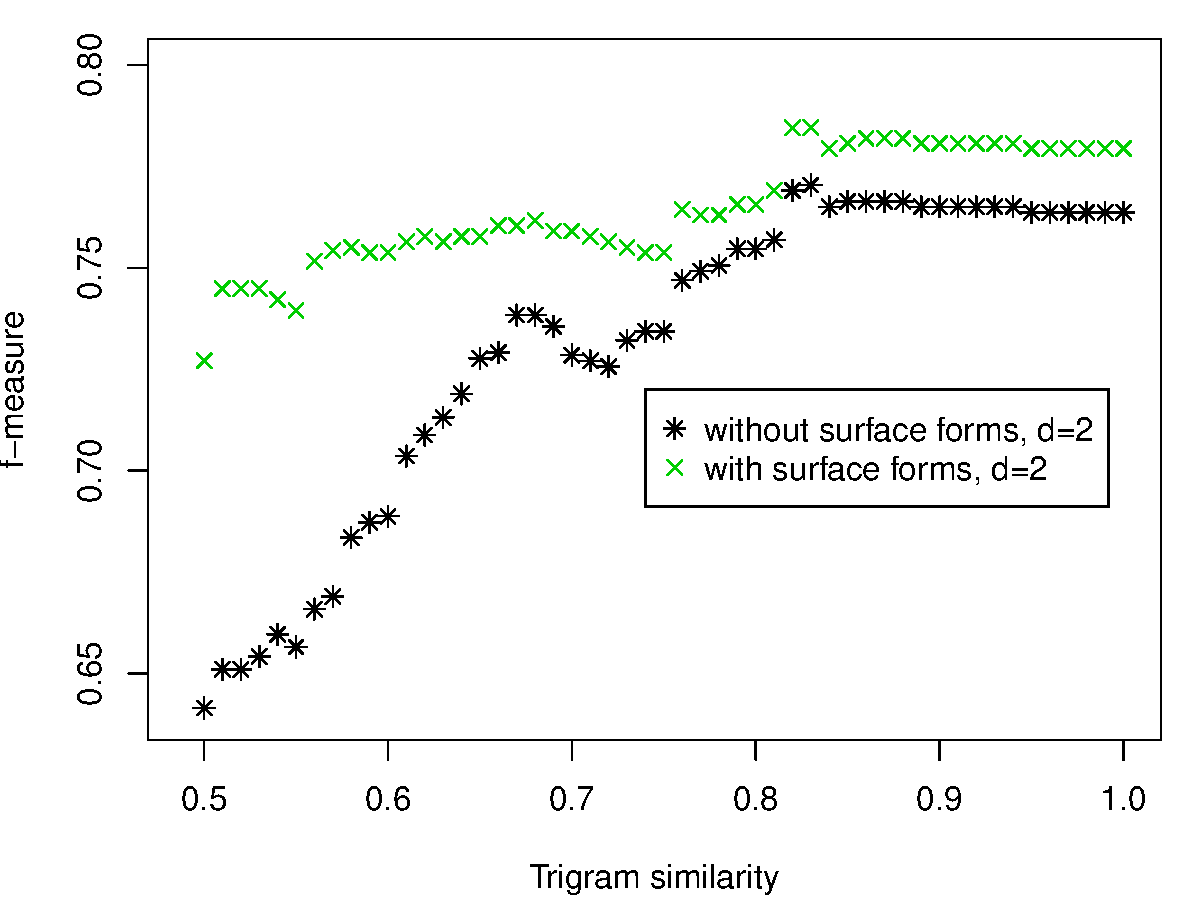
\includegraphics[width=0.9\linewidth]{fig/reutersWithoutSurfaceFormsAndBFS2.pdf}
        %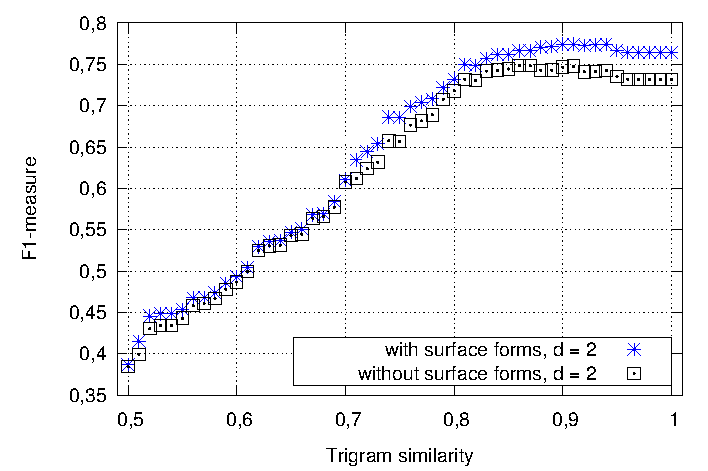
\includegraphics[width=0.9\linewidth]{fig/surface_forms_diag.pdf}
%    \caption{Influence of surface forms on the Reuters-21578 corpus and DBpedia as \ac{KB}.}\label{fig:influenceOfSurfaceForms}
%\end{figure}
%\todo[inline]{@axel: not using any graph just trigram sim is worse than the rest}
% for AGDISTIS are worse since our approach could not make use of surface forms as explained above. %, redirects or disambiguation entities, as explained above.
%Yet, given that a 1-1 mapping exists between YAGO2 and DBpedia URIs, we will consider the results of DBpedia for AGDISTIS in the following comparisons with other tools.
%\todo[inline}]{AN:Formally wrong. Either a 1-1 mapping exists or it does not}
%If there is no 1-1 mapping, the result of the disambiguation is counted as \emph{false positive}, which then results in low \mbox{F-measures} using YAGO2 as \ac{KB}.
%\todo{look at table caption please}


%\textbf{Comparison with AIDA.} 
%\todo[inline]{renew numbers}
%We compared our approach to AIDA by using the \textit{Cocktailparty configuration}\footnote{\url{https://github.com/yago-naga/aida}} (which is the recommended configuration for the framework) and applied the same restrictions that we used for AGDISTIS.
%The results of this evaluation on AIDA can be seen in Table~(\todo[inline]{here was a reference to the eval result}).
%Overall, AIDA performs well on arbitrary entities. 
%Yet, it is clearly outperformed by our approach on specific persons and organizations. 
%\todo[inline]{the statement above cant be seen in table 4, therefore we need to compare by type or clarify this sentence}
%In comparison to AIDA, AGDISTIS performs best on the Reuters-21578  where it surpasses AIDA by $\approx 0.16$ \mbox{F-measure}.
%Here AGDISTIS benefits from surface forms and its expansion policy.
%Furthermore, AGDISTIS outperforms AIDA with the RSS-500 corpus by $\approx 0.15$ \mbox{F-measure}.
%This corpus differs considerably from the Reuters-21578 corpus due to the small disambiguation contexts and graphs evolving from two named entities per text only.
%Note that AGDISTIS also outperforms AIDA for our overall default setting of $\sigma = 0.81$, apart from the result on the AIDA-YAGO2 corpus.
%AIDA could not be run on the \url{news.de} corpus as it can only deal with English.
%Here, the \emph{language-independence} of AGDISTIS provides a significant improvement of the state of the art.
%AIDA performs better on AIDA-YAGO2 achieving an \mbox{F-measure} of 0.83 due to the large contexts of the documents (see Table~(\todo[inline]{here was a reference to a data table})).
%This is clearly due to AGDISTIS being tuned towards smaller contexts since these are more common in WND, see Table~(\todo[inline]{here was a reference to a data table}).
%In particular, the AIDA-YAGO2 corpus contains many sport teams from cities and countries like \texttt{Barcelona} where AGDISTIS identifies \texttt{dbr:Barcelona} and \texttt{dbr:FC\_Barcelona} as resources. Since \texttt{dbr:Barcelona} has a higher authoritative score than \texttt{dbr:FC\_Barcelona}, AGDISTIS' disambiguation results in a \emph{false positive} in this particular case.
%As shown in Table~\ref{eval} using YAGO2 leads to worse results since AGDISTIS (in contrast to AIDA) does not possess surface forms for YAGO2.
%\todo[inline]{No appendiy, how to solve this?}

%\textbf{Comparison with DBpedia Spotlight.}
%\todo[inline]{renew the numbers}
%In order to compare DBpedia Spotlight with AGDISTIS Cornolti et al.~\cite{cornolti} used Spotlight's Web services.\footnote{\url{https://github.com/dbpedia-spotlight/dbpedia-spotlight/wiki/Web-service}}

%The results of the evaluation are shown in Table~\ref{tab:eval}.
%Spotlight performs best on the \url{news.de} dataset (\mbox{F-measure} = 0.84) and worst on the Reuters-21578 dataset (\mbox{F-measure} = 0.56), Table~(\todo[inline]{here was a reference to the eval result}).
%This is possibly due to the datasets age of over 20 years and missing historic data in DBpedia.
%When evaluated against the AIDA-YAGO2 corpus Spotlight achieves a \mbox{F-measure} of 0.57.
%Using the RSS-500 dataset Spotlight is only able to generate a \mbox{F-measure} of 0.56.
%\todo[inline]{renew the number}
%AGDISTIS outperforms Spotlight by at least $\approx 0.15$ \mbox{F-measure}. % using DBpedia as \ac{KB}. on each English dataset.

%AGDISTIS performs better on two of the datasets and is even usable for the German dataset as it is agnostic towards the language of the used \ac{KB}.
%As can be seen in Figure \ref{fig:relation} the number of entities per text is an important criteria for disambiguation.

%\textbf{Run time analysis.}
%On average AGDISTIS is more time-efficient than AIDA with respect to the best %corresponding configuration.
%While AGDISTIS finished its computation on Reuters-21578 corpus in 549\,seconds (s), AIDA needed more than twice as much time,\,i.e., 1,296\,s.
%This behavior can also be seen on the short documents of the RSS-500 dataset, where AIDA needed 4,919\,s and our approach only 623\,s.
%Moreover, AGDISTIS outperforms AIDA with 3,946\,s to 51,435\,s run time on the AIDA-YAGO2 corpus.
%\todo[inline]{is not comparable anymore since we needed to run it in the cloud}
%Details can be found on the project website.



%\subsection{English and German Evaluation.} AGDISTIS has been evaluated on 9 different datasets from diverse domains such as news, sports or buisiness reports.
%For English datasets AGDISTIS is able to outperform the currently best disambiguation framework, TagMe2, on three out of four datasets by up to 29.5\% F-measure. 
%Considering the only German dataset available for named entity disambiguation, i.e., \url{news.de}~\cite{n3}, we are able to outperform the only competitor DBpedia Spotlight by 3\% F-measure.

%\subsection{How the Chinese version was generated}



%However, the latest available Linked Data --- DBpedia 3.9 --- has no such information for Chinese. 
%Therefore, we created triples containing \texttt{\ac{RDF}:type} as predicate by translating the English ones to Chinese. 
%Specifically, we use inter-language links extracted by DBpedia 
%\footnote{Available from \url{http://wiki.dbpedia.org/Downloads39\#inter-language-links}}, in which a English resource is represented in different other languages. 
%An English-Chinese pair of phrases for each resource is extracted using the following regular expression\footnote{{\it zh} is the language code for Chinese.}:
%\begin{verbatim}
%``$\langle http://dbpedia\backslash.org/resource/(.*)\rangle\backslash s*\langle.*\rangle \backslash s*\langle http://zh.dbpedia.org/resource/(.*)\rangle\backslash s*.$"
%\end{verbatim}
%, resulting a phrase table with 420,047 English-Chinese pairs.

%For each \ac{RDF}:type triple in the English DBpedia, if the name of the subject appears in the phrase table, it is mapped to Chinese according to the phrase table. In this way, a total of 1,234,783 triples are extrated for Chinese.

%Both the data stored in a Lucene 4.5.1 Index and the phrase table can be found at \url{http://139.18.2.164/rusbeck/}.

%\subsection{Accuracy results of the Chinese version}
%In this section, we will introduce a new Chinese benchmark and the evaluation results.

\subsection{Chinese Benchmark}
\label{sec:chinese}
The key to extend AGDISTIS to support a new language, in this case Chinese, is to provide the needed \ac{RDF} data for this particular language, especially \texttt{rdf:type} information. 
To evaluate the Chinese version of AGDISTIS, a Chinese benchmark has been created in the context of \ac{QA}.
The disambiguation of named entities is a key step to answer natural language questions based on Linked Data. 
%\subsubsection{Results}

%\noindent \textbf{Chinese Evaluation.} We evaluated the Chinese version of AGDISTIS within a question answering setting. 
To this end, we used the multilingual benchmark provided in QALD~4~\cite{qald4}. 
Since the Chinese language is not supported, we extended the QALD~4 benchmark by translating the English questions to Chinese and inserted the named entity links manually.
%The accuracies achieved by AGDISTIS for the train and test datasets are 65\% and 70\% respectively. 
%We also performed a fully automatic evaluation by using the Chinese segmentation and named-entity recognition algorithms provided by LTP-Cloud\footnote{\url{http://www.ltp-cloud.com/}}. 
%The accuracies sank to 32\% and 38\%.
%These results indicate the need for better resources for Entity Recognition in Chinese.

We first report the disambiguation accuracies by assuming the named entities are given. It allows a fair comparison to other disambiguation algorithms because named entity disambiguation performance is highly depended on named-entity recognition results. The accuracy is measured at a sentence level by assuming a correct disambiguation should recognize and link all the entities in a sentence, which is essential for further steps in question answering. The accuracies for the training and testing are 65\% and 70\% respectively. 

%We also performance a fully automatic evaluation by using the Chinese segmentation and named-entity recognition algorithms provided by LTP-Cloud\footnote{\url{http://www.ltp-cloud.com/}}. 
%The accuracies are 32\% and 38\%.


 
\section{Demonstration}
%\begin{itemize}
%\item Moreover, the output format of AGDISTIS will be explained. 
%An online version of the demo is available at \url{http://agdistis.aksw.org/demo}.
%The aim of this demo is to present the English, German and Chinese version of our framework based on DBpedia.
%\item A demo of our approach (integrated into the Named Entity Recognition framework FOX~\cite{FOX}) can be found at \url{http://fox.aksw.org}. 
%\item In this demo, we will present AGDISTIS deployed on three different languages (English, German and Chinese) and three different knowledge bases (DBpedia, the German DBpedia and the Chinese DBpedia).
%To the best of our knowledge, we therewith provide the first Chinese instantiation of entity linking to DBpedia.
%\item We will also demonstrate the AGDISTIS web services endpoints for German, English and Chinese disambiguation and show how data can be sent to the endpoints.
%\item Moreover, the output format of AGDISTIS will be explained.
%
%\end{itemize}

Within our demonstration, we aim to show how AGDISTIS can be used by non-expert as well as expert users. \footnote{An online version of the demo is available at \url{http://agdistis.aksw.org/demo}.}
Another aim of this demo is to present the English, German and Chinese version of our framework based on DBpedia.
For non-experts, we provide a graphical user interface (GUI).
Experts can choose to use the REST interfaces provided by the tool. % or use a Java snippet to call the REST interface.
The whole of this functionality, which will be described in more details in the following. % sections, will also be demonstrated at the conference.

\subsection{AGDISTIS for non-expert users}
A screenshot of the AGDISTIS GUI is shown in Figure~\ref{fig:gui}.
This GUI supports the following workflow.

\begin{figure}[htb!]
\centering
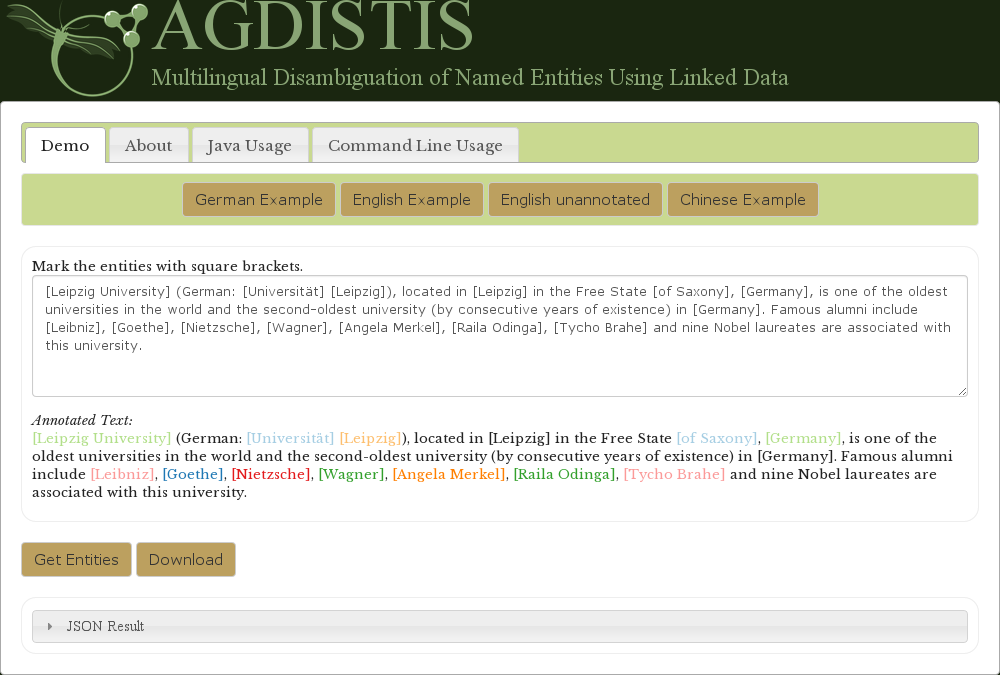
\includegraphics[width=\textwidth]{part_02/unstructured_annotation/fig/GUI.png}
\caption{Screenshot of the demo with an English example which is already annotated.}
\label{fig:gui}
\end{figure}

\noindent\textbf{Entity Recognition}
After typing or pasting text into the input field, users can choose between either annotating the entities manually or having the entities detected automatically.
In the first case, the labels of the entities are to be marked by using square brackets, see central panel of Figure~\ref{fig:gui}.
In the case of an automatic annotation, we send the text to the FOX framework, which has been shown to outperform the state of the art in~\cite{FOX}.
%In our current implemen
%Since there is no multilingual \ac{NER} tool available, an automatic annotation of entities works only for English texts.
%We will demonstrate this feature by using both manually pre-annotated text and text without annotations in our examples (see upper bar of Figure~\ref{fig:gui}).
%Moreover, we will allow the crowd to enter arbitrary texts that pertain to their domain of interest.

\noindent\textbf{Automatic Language Detection}
Once the user has set which entities are to be disambiguated, the marked-up text is sent to the language detection module based on~\cite{nakatani2010langdetect}.
We chose this library because it is both precise ($>99\%$ precision) and time-efficient.
If the input is detected to belong to one of the languages we support (i.e., German, Chinese, English), then we forward the input to a dedicated AGDISTIS instance for this given language.
In all other cases, an error message is shown to the user, pointing towards the language at hand not being supported.
The main advantage of this approach is that the user does not need to select the language in which the text is explicated manually, thus leading to an improved user experience. 
%We will demonstrate this feature by entering text in different languages (German, English, French, Chinese, etc.) and presenting the output of the framework for each of these test cases.

\noindent\textbf{Entity Linking} 
This is the most important step of the whole workflow.
The annotated text is forwarded to the corresponding language-specific deployment of AGDISTIS, of which each relies currently on a language-specific version of DBpedia 2014. 
%The approach underlying AGDISTIS~\cite{agdistis_iswc} is language-independent and combines breadth-first search and the well-known  \ac{HITS} algorithm. 
%In addition, string similarity measures and label expansion heuristics are used to account for typos and morphological variations in naming.
%Moreover, Wikipedia-specific surface forms for resources can be used. 

\noindent\textbf{Output}
Within the demo the annotated text is shown below the input field where disambiguated entities are colored to highlight them. 
While hovering a highlighted entity the disambiguated URI is shown.
We will demonstrate the output of the entity linking by using the examples shown in the upper part of Figure~\ref{fig:gui}. 
The output of the system will be shown both in a HTML version and made available as a download in JSON. 
%Moreover, we will allow interested participants to enter their own examples and view the output of the tool.

\subsection{AGDISTIS for expert users}

%To support different languages, we set up a REST URI for each of the language versions.
%those\footnote{\url{http://139.18.2.164:8080/AGDISTIS_DE}}\footnote{\url{http://139.18.2.164:8080/AGDISTIS_ZH}}\footnote{\url{http://139.18.2.164:8080/AGDISTIS}}.
Each of these endpoints understands two mandatory parameters: (1) \texttt{text} which is an UTF-8 and URL encoded string with entities annotated with XML-tag \texttt{<entity>} and (2) \texttt{type='agdistis'} to disambiguate with the AGDISTIS algorithm.
In the future, several wrappers will be implemented to use different entity linking algorithms for comparison.
Following, a CURL\footnote{\url{http://curl.haxx.se/}} snippet shows how to address the web service, see also \url{http://agdistis.aksw.org}:
\begin{verbatim}
curl --data-urlencode "text='<entity>Barack Obama</entity> arrives 
in <entity>Washington, D.C.</entity>.'" -d type='agdistis' 
{AGDISTIS URL}/AGDISTIS
\end{verbatim}


%architecture, what are the main steps
%GOAL is to provide entity linking results to several languages which are show on the website and downloadable as JSON
%1 we will present and explain how AGDISTIS works and how multilinguality is achieved
%2 Users can try different inputs at the demo station and tell us, what quality they expect and which languages they want
%3 finally we will show how the results can be downloaded or seen online and how the annotation of more or less entities changes the behaviour of AGDISTIS
%benchmarks will be shown as well and people will be invited to use our for free endpoint for their projects so we can store the use case data and improve our approach similar to the feedback API of spotlight and fox

\chapter{Type Annotation on Unstructured Texts}
\label{cha:cetus}
\graffito{
This chapter presents CETUS, a pattern-based approach for annotating \ac{RDF} type information to entities.
CETUS has won the OKE challenge 2015~\cite{okechallenge}, task 2, and is published in~\cite{CETUS_2015}.
The author of this thesis assisted the main author in programming, co-wrote the paper and its poster. 
}


Standard document processing pipelines miss the opportunity to gain insights from semantic entities novel to the underlying \ac{KB}. 
That is, most known tool chains recognize entities based on linguistic models and link them to a \ac{KB} or null if they are emerging entities. 
So far, linking novel entities has only been the concern of a few approaches~\cite{AIDA,agdistis_iswc}.
Consequently, extracting type information for emerging and existing entities is a novel research avenue so far only tackled by the TAC KBP \ac{EL} challenge 2014\footnote{\url{http://nlp.cs.rpi.edu/kbp/2014/}}, the Micropost workshop series\footnote{\url{http://www.scc.lancs.ac.uk/microposts2015/}} and the OKE challenge 2015~\cite{okechallenge}.

We present CETUS, a novel pattern based entity type extraction tool for identifying the type of a given entity inside a given text and linking this type to a \ac{KB}, i.e., to the subset of the DOLCE+DnS Ultra Lite ontology classes\footnote{\url{http://www.ontologydesignpatterns.org/ont/dul/DUL.owl}}.
Here the subset refers to \texttt{dul:Person}, \texttt{dul:Place}, \texttt{dul:Organization} and \texttt{dul:Role}.
CETUS' pipeline is divided into three subsequent parts: i) an a-priori pattern extraction, ii) a grammar-based analysis of the input document and iii) a mapping of the type evidence to the DOLCE+DnS Ultra Lite classes. 
Our contributions are as follows:
\begin{itemize}
\item CETUS is a fast and easy to implement baseline approach to path a way to novel research insights.
\item Our approach implements two approaches for the third step using the YAGO ontology as well as the FOX~\cite{FOX} \ac{NER} tool.
\item CETUS outperforms other apprroaches~\cite{okechallenge} w.r.t. the OKE challenge 2015 and thus is able to generate novel \ac{RDF} data from unstructured text.
\end{itemize}

In the following, we will explain these parts in detail and conclude in Section~\ref{cha321:sec:conclusion}. 
The open source code of CETUS can be found at \url{https://github.com/AKSW/Cetus}.
\section{Pattern Extraction}
\label{sec:patternExt}

The patterns used for identifying the type of an entity inside a document, are generated semi-automatically in an iterative manner.
First, CETUS identifies phrases containing entities and their types in a given document corpus (here we use the DBpedia 2014 abstracts) and extracts them.
After sorting these phrases according to the string in between the entity and its type, we analyze them and create the patterns in an incremental process.
The progress of our pattern extraction is measured by the amount of phrases that are covered by our patterns.
In the following, these steps are described in more detail.

\subsection{Sentence Part Extraction}

For extracting the phrases containing entities and their types, we used the abstracts of the English DBpedia 2014 abstracts dump file.
Every abstract describes the entity it belongs to and, thus, contains the label of the entity and its type.
We assume, abstracts are written properly and thus contain both information.

First, CETUS preprocesses each abstract individually.
Our approach removes the text written in brackets, e.g., pronunciations.
%Afterwards, we use the Stanford Deterministic Coreference Resolution System~\cite{Lee2013} to replace pronouns with their coreferenced words, e.g., \emph{He studied physics} with \emph{Albert Einstein studied physics}.
Next step of the preprocessing is the splitting of the abstracts into single sentences.
%\todo[inline]{@Micha: still valid?}
Second, sentences containing the entity label and at least one label of one of its types (\texttt{rdf:type}) are processed further.
CETUS extracts the part of the sentence between the entity label and the type label and stores additionally the words, their lemmas and part-of-speech tags of the extracted phrase.

After analysing all abstracts, CETUS counts the different phrases.
The words inside these parts are encoded as \texttt{<word>\_<lemma>\_<pos-tag>}.
Table~\ref{tab:extParts} shows examples of extracted phrases and their counts how often they have been found inside the English DBpedia.

Delving into the extracted phrases reveals insights into the structure of entity type descriptions in DBpedia abstracts.
That is, the formulation "\texttt{<entity>} \emph{is a} \texttt{<type>}" occurs most often.
%The second most common formulation is nearly the only one in our list, in which the type precedes the entity.
The second most common formulation uses a type preceding the entity and is listed as the second example in Table~\ref{tab:extParts}.
The third example is a variant of the first one containing the determine "an" instead of "a".
The fourth example shows that some abstracts contain more complex formulations like "\texttt{<entity>} \emph{is a} \texttt{<type>} \emph{of} \texttt{<type>}" while the last example contains an additional adjective that was not a part of the types label, i.e., "flowering".

\begin{table}[htb!]
\centering
\resizebox{\textwidth}{!}{
\begin{tabular}{lp{5mm}r}
 \toprule
 \multicolumn{1}{c}{\textbf{Extracted phrase}} && \multicolumn{1}{c}{\textbf{Count}} \\
 \midrule
 \texttt{<entity> is\_be\_vbz a\_a\_dt <type>} && 242\,806 \\
 \texttt{<type> <entity>} && 107\,082 \\
 \texttt{<entity> is\_be\_vbz an\_an\_dt <type>} && 12\,981 \\
 \texttt{<entity> is\_be\_vbz a\_a\_dt species\_species\_n1 of\_of\_pp-f <type>} && 12\,554 \\
 \texttt{<entity> is\_be\_vbz a\_a\_dt species\_species\_n1} && \multirow{2}{*}{4\,069} \\ 
 \qquad\qquad\ \ \texttt{of\_of\_pp-f flowering\_flower\_j-vvg <type>} && \\
 \bottomrule
\end{tabular}
}
\caption{Examples of sentence parts found between an entity and its type.}
\label{tab:extParts}
\end{table}

\subsection{Grammar Construction}
\label{sec:grammar}

The aim of creating a grammar is to generate a parser that is able to identify the part of a sentence describing  the type of an entity,
The parser is based on the given position of the entity inside the sentence.
For generating a parser based on our grammar, we are using the ANTLR4 library\footnote{\url{http://www.antlr.org/}}.

Our grammar is based on the following assumptions:
\begin{enumerate}
\item A sentence contains an entity and a type. Otherwise the sentence is not part of our grammar language.
\item A type must contain a noun, but can contain additional words that are specifying the meaning of the noun, e.g., adjectives.
%Note, that the type is not a noun phrase!
\end{enumerate}

The first assumption simplifies the task of defining a grammar since we can focus on the sentences that are important for our task and ignore all others.
The second assumption contains the definition of a type surface form.
It might seem to be contradictory w.r.t. the last example of Table~\ref{tab:extParts} but for the extraction it is important that we extract all words that \emph{could} be part of the types surface form.
Following this assumptions, we can define a type inside the grammar with the rule in Listing~\ref{lst:typeRule}.

\lstset{
%  basicstyle=\footnotesize\ttfamily,
%  breaklines=true,
%  captionpos=b,                    % sets the caption-position to bottom
%  frame=single,
%  %morecomment=[s][\color{blue}]{<}{>},
%  morecomment=[s][\color{red}]{"}{"},
  numbers=none
%  
%%  numbersep=5pt,
%% numberstyle=\tiny,
%%  stringstyle=\tiny
}

\begin{figure}[htb!]
\begin{lstlisting}[label=lst:typeRule, caption=The grammar rule defining a type surface form.]{typeRule}
type : (ADJECTIVE|VERB|ADVERB)* FOREIGN? NOUN+;
\end{lstlisting}
\end{figure}

A surface form of a type can contain a number of adjectives, verbs or adverbs as well as a foreign word, e.g., the latin word "sub".
Additionally, a type has one or more nouns.

As mentioned above, the construction of the grammar is designed to be an iterative, incremental, self-improving process.
We start with the simple \emph{is-a} pattern that matches the most common phrase "\texttt{<entity>} \emph{is a} \texttt{<type>}". 
The definition of this pattern is shown in Listing~\ref{lst:firstIsARule}.
\begin{figure}[htb!]
\begin{lstlisting}[label=lst:firstIsARule,caption=First simple version of the \emph{is-a} pattern. \texttt{ENTITY} marks the position of an entity.]{firstIsARule}
is_a_pattern : ENTITY is_is_vbz a_a_dt type;
\end{lstlisting}
\end{figure}

With this simple grammar, we try to match all phrases extracted beforehand and create a list containing all those phrases that have not been matched so far.
Using this list, we extend our grammar to match other phrases.
In our example, we extend the simple \emph{is-a} pattern towards matching different temporal forms of the verb "be" and different determiners, e.g., "a" and "an", see Listing~\ref{lst:secondIsARule}.


\begin{figure}[htb!]
\begin{lstlisting}[label=lst:secondIsARule,caption=Extended version of the \emph{is-a} pattern.]{secondIsARule}
is_a_pattern : ENTITY FORM_OF_BE DETERMINER <type>

FORM_OF_BE : ~[ \t\r\n]+ '_be_v' ~[ \t\r\n]*;
DETERMINER : ~[ \t\r\n]+ '_' ~[ \t\r\n]+ '_d' ~[ \t\r\n]*;
\end{lstlisting}
\end{figure}

With this iterative, incremental process, we further extended the grammar until we covered more than 90\% of the extracted phrases.
The complete grammar can be found in the projects source code repository.

%\subsection{Example Patterns}

%\todo[inline]{Should we keep this section or delete it?}

%\begin{figure}
%\begin{lstlisting}[label=lst:allPatternRules,caption=The grammar rules for finding a type surface form.]{allPatternRules}
%sentence : WORD* ENTITY (COMMA (WORD|POINT|COMMA|COLON)+ COMMA)? type_after_entity_pattern (WORD|POINT|COMMA|COLON)*
%| WORD* type_in_front_of_entity ENTITY WORD*;
%
%type_after_entity_pattern : is_a_type_of_pattern
%| is_a_pattern
%| type_with_dt ;
%
%is_a_pattern : FORM_OF_BE type_with_dt (((COMMA? AND) | COMMA) type_with_dt)*;
%is_a_type_of_pattern : FORM_OF_BE type_with_dt OF type_with_dt;
%
%type_in_front_of_entity : type_with_dt (OF|COMMA|COLON)?;
%
%type_with_dt : DETERMINER? nr_or_crd? type;
%nr_or_crd : NUMBER | CARDINAL_NUMBER;
%\end{lstlisting}
%\end{figure}

\section{Type Extraction}
\label{sec:docAnalysis}

The pattern-based type extraction can be separated into two steps.
The first step extracts type evidence strings from the text, while the second step creates a local type hierarchy based on the extracted string.
Following, we describe both steps in more detail.

\subsection{Type String Extraction}

To identify the type evidence string for a certain entity, CETUS extracts the string containing the type of a given entity from a given text using the grammar from above.
Let us assume the following running example: 

\begin{center}
\emph{\textbf{Albert Einstein} was a German-born theoretical physicist. In 1921, he got the Nobel Prize in Physics. }
\end{center}

CETUS processes the document as input with "Albert Einstein" marked as entity.
The text is split into sentences and the surface form of the entity is replaced by a placeholder. 

\begin{center}
\emph{\textbf{ENTITY} was a German-born theoretical physicist.}

\emph{In 1921, he got the Nobel Prize in Physics.}
\end{center}

A parser based on the grammar from Section~\ref{sec:grammar} is applied to every sentence.
While the second sentence is identified as not contained in the language of the grammar, the first sentence is identified to be in the language.
Here, we discard the second sentence from further processing, although a co-reference resolution~\cite{NgongaNgomo2014} approach could increase the performance in other cases.
Moreover, the parser identifies "German-born theoretical physicist" as evidence type string.

\subsection{Local Type Hierarchy}

Based on the extracted evidence type string, CETUS creates a type hierarchy and links the given entity to the hierarchy.
The type hierarchy comprises classes that are generated automatically from the extracted string based on the second assumption of Section~\ref{sec:grammar}.
Each class is generated by concatenating the words found in the extracted string using camel case.
After a class has been created, the first word is removed and the next class is created.
Every following class is a super class of the classes generated before.
Finally, the entity is connected to all generated classes.

For our example, three classes would be generated and linked to the entity as shown in Listing~\ref{lst:localHierarchy} respectivly Figure~\ref{fig:localHierarchy}.%\footnote{The prefix \texttt{ex} could stand for every user defined vocabulary, e.g., \url{http://example.com/}.}.

\begin{figure}[htb!]
\centering
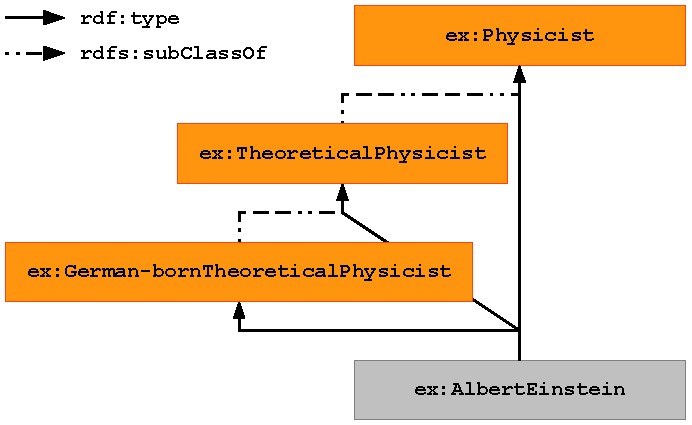
\includegraphics[scale=0.75]{part_02/unstructured_annotation/fig/localHierarchy.pdf}
\caption{Schema of the generated local hierarchy of the example.}
\label{fig:localHierarchy}
\end{figure}

\begin{figure}[htb!]
\begin{lstlisting}[label=lst:localHierarchy,caption=The local hierarchy is generated from the extracted string expressed using Turtle as \ac{RDF} serialization.]{localHierarchy}
ex:AlbertEinstein
    a ex:German-bornTheoreticalPhysicist, 
        ex:TheoreticalPhysicist, ex:Physicist .

ex:German-bornTheoreticalPhysicist
    a rdfs:Class ;
    rdfs:subClassOf ex:TheoreticalPhysicist ;
    rdfs:label "German-born theoretical physicist" .

ex:German-TheoreticalPhysicist
    a rdfs:Class ;
    rdfs:subClassOf ex:Physicist ;
    rdfs:label "theoretical physicist" .

ex:German-Physicist
    a rdfs:Class ;
    rdfs:label "physicist" .

\end{lstlisting}
\end{figure}

\section{Entity Type Linking using YAGO}
\label{sec:linkingyago}

%CETUS approach to link the evidence string to the DOLCE+DnS Ultra Lite classes \texttt{dul:Person}, \texttt{dul:Place}, \texttt{dul:Organization} and \texttt{dul:Role} is twofold.

The linking of the generated classes to a \ac{KB} can be done in two different ways.
Our first approach, CETUS$_{YAGO}$,  uses the labels of the automatically generated classes to find a matching class inside another, well-known \ac{KB}.
CETUS uses the YAGO ontology~\cite{mahdisoltani2014yago3} which comprises a large class hierarchy and, thus, increases the chance to match one of these classes.
YAGO itself contains more than 10 mio. entities and exceeds 350.000 classes.
Our second approach serves as a baseline to our own approach and uses the FOX~\cite{FOX} tool.

First, we created an index containing the surface forms of the YAGO classes with a mapping to the class URIs.
Second, CETUS needs to match every generated class using the approach from Section~\ref{sec:docAnalysis} to one of the labels of the YAGO classes.

Currently, our approach uses 3-gram string similarity to match labels in the index with those of the generated classes as it has been proven to be efficient and effective for such a task~\cite{agdistis_iswc}.
This process retrieves most similar YAGO class for every generated class and a similarity score.
From these YAGO classes, CETUS chooses the class with the highest similarity score.
If two classes have the same score, CETUS chooses the class which is lower inside the local generated type hierarchy.
The chosen YAGO class is linked to its local class.

After that, we iterate through the YAGO class hierarchy from the linked class to its root, searching for one of the classes listed in Table~\ref{tab:yagoClassMatching}.
If such a class is found, we link it with the corresponding DOLCE+DnS Ultra Lite class.
Otherwise, we repeat the search using the YAGO class with the second highest similarity score.
The result for our running example can be seen in Figure~\ref{fig:localYAGOHierarchy}
\begin{table}[htb!]
\centering
\begin{tabular}{lp{5mm}l}
\toprule
 \multicolumn{1}{c}{YAGO class} && DOLCE+DnS Ultra Lite class \\
\midrule
 \texttt{yago:wordnet\_person\_100007846} && \texttt{dul:Person} \\
 \texttt{yago:wordnet\_location\_100027167} && \texttt{dul:Place} \\
 \texttt{yago:wordnet\_organization\_108008335} && \texttt{dul:Organization} \\
 \texttt{yago:wordnet\_role\_100722061} && \texttt{dul:Role} \\
\bottomrule
\end{tabular}
\caption{Mapping from YAGO to DOLCE+DnS Ultra Lite classes.}
\label{tab:yagoClassMatching}
\end{table}

\begin{figure}[htb!]
\centering
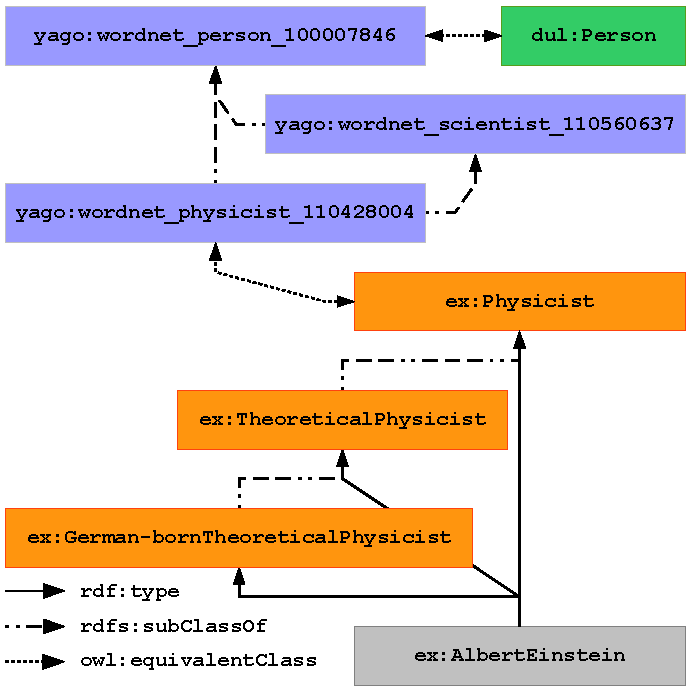
\includegraphics[scale=0.75]{part_02/unstructured_annotation/fig/localYAGOHierarchy.pdf}
\caption{Resulting type hierarchy that is created based on the YAGO ontology.}
\label{fig:localYAGOHierarchy}
\end{figure}

%\begin{table}
%\centering
%\begin{tabular}{@{}ll@{}}
%\toprule
%\textbf{Similarity} & \textbf{Formula/Explanation} \\ \midrule
%Dice-Coefficient Similarity &         \\
%Levenstein/Edit Similarity &         \\
%Euclidean Similarity &         \\ 
%Semantic Similarity &      Word2Vec   \\\bottomrule
%\end{tabular}
%\caption{Similarity measures of CETUS}
%\label{tab:stringsim}
%\end{table}

%CETUS' algorithms are easily extensible via its interfaces. 
%We will refine the set of string matching algorithms after the evaluation against the Open Knowledge Extraction task 2 corpora.

\section{Entity Type Linking using FOX}
\label{sec:typeLinking}
\begin{table}
\centering
\begin{tabular}{lp{5mm}l}
\toprule
 \multicolumn{1}{c}{FOX class} && DOLCE+DnS Ultra Lite class \\
\midrule
 \texttt{scmsann:PERSON} && \texttt{dul:Person} \\
 \texttt{scmsann:LOCATION} && \texttt{dul:Place} \\
 \texttt{scmsann:ORGANIZATION} && \texttt{dul:Organization} \\
 %\texttt{scmsann:OTHER} && \texttt{dul:Role} \\
\bottomrule
\end{tabular}
\caption{Mapping from FOX classes to DOLCE+DnS Ultra Lite classes.}
\label{tab:foxclassmatching}
\end{table}


A second approach for a type extraction baseline is the usage of one of the various, existing entity typing tools.
For our second version CETUS$_{FOX}$, we are using FOX, a \ac{NER} and typing tool based on ensemble learning over 8 different tools.

CETUS$_{FOX}$ sends the given document to the FOX web-service for retrieving annotations.
If the entity inside the document is found and typed by FOX, the type is used to choose one of the four DOLCE+DnS Ultra Lite classes, see Table~\ref{tab:foxclassmatching}.
The chosen class is used as super class for the automatically created classes.
Unfortunately, FOX does not identify roles in its current version.

With respect to our running example, the FOX tool marks "Albert Einstein" as a person.
Thus, the created classes would be defined as subclasses of \texttt{dul:Person} as shown in Figure~\ref{fig:localFOXHierarchy}.

\begin{figure}[htb!]
\centering
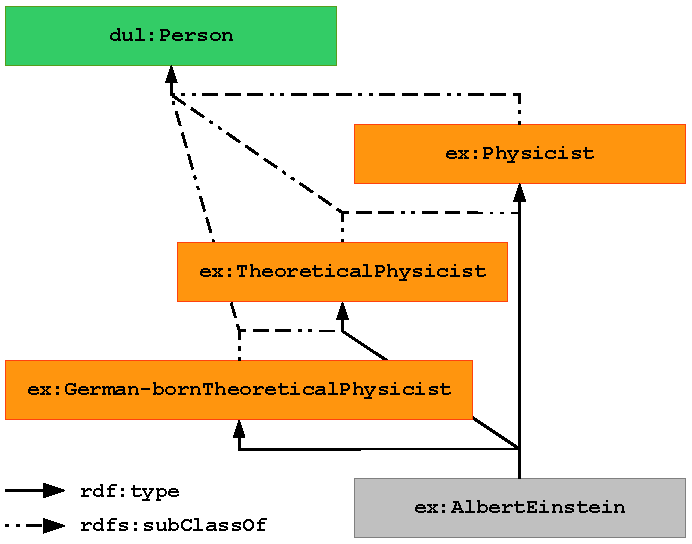
\includegraphics[scale=0.75]{part_02/unstructured_annotation/fig/localFOXHierarchy.pdf}
\caption{Resulting type hierarchy that is created based on the results of FOX.}
\label{fig:localFOXHierarchy}
\end{figure}

%
%\usepackage{graphicx}
%\usepackage{subfigure}
%\usepackage{amsmath,amssymb}
%\usepackage[english]{babel}
%\usepackage[utf8]{inputenc}
%\usepackage[ruled,vlined]{algorithm2e}
%\usepackage{url}
%\usepackage{float}
%\usepackage{multirow} 
%\usepackage{booktabs}
%\usepackage[disable]{todonotes}
%\usepackage{todonotes}
%\usepackage{booktabs}
%\usepackage{mdframed}
%\usepackage{wrapfig}
%\usepackage{caption}
%\usepackage{tikz}
%\usepackage{verbatim}
%\usepackage{afterpage}
%\usepackage[active,tightpage]{preview}
%\PreviewEnvironment{tikzpicture}
%\setlength\PreviewBorder{5pt}%

%\usepackage{siunitx}%number formatting inside tables
\sisetup{
round-mode = places,
detect-family = true,
detect-inline-family = math,
detect-weight=true,
detect-inline-weight = math
}%

%\begin{document}


\chapter{Cross-Document Co-reference Resolution using Latent Features}


%\author{
%Axel-Cyrille Ngonga Ngomo$^{\diamondsuit}$ \and
%Michael R\"oder$^{\spadesuit\diamondsuit}$ \and 
%Ricardo Usbeck$^{\spadesuit\diamondsuit}$ 
%\institute{
%${\diamondsuit}$ University of Leipzig, Germany, 
%${\spadesuit}$ R\,\&\,D, Unister~GmbH, Leipzig, Germany, 
%\newline email: \{ngonga$|$usbeck\}@informatik.uni-leipzig.de
%}
%}

%\maketitle

%\newmdtheoremenv{ex}{Example}
\newcommand{\goodgap}{%
%\hspace{\subfigtopskip}%
%\hspace{\subfigbottomskip}
}
\todo[inline]{adjust goodgap}
%\begin{abstract}
Over the last years, entity detection approaches which combine named entity recognition and entity linking have been used to detect mentions of RDF resources from a given reference knowledge base in unstructured data. In this paper, we address the problem of assigning a single URI to named entities which stand for the same real-object across documents but are not yet available in the reference knowledge base. This task is known as cross-document co-reference resolution and has been addressed by manifold approaches in the past. We present a preliminary study of a novel take on the task based on the use of latent features derived from matrix factorizations combined with parameter-free graph clustering. 
%We study whether this approach achieves better results than the simple approaches used in most tools so far by measuring the accuracy of the clusters we detect on several benchmark datasets.
We study the influence of different parameters (window size, rank, hardening) on our approach by comparing the F-measures we achieve on the $\mbox{N}^3$ benchmark.
Our results suggest that using latent features leads to higher F-measures with an increase of up to 20.5\% on datasets of the $\mbox{N}^3$ collection.
%\end{abstract} 

%\todo[inline]{Full paper with a maximum of 12 pages including references
%Short paper with a maximum of 6 pages including references}

\section{Introduction}
%\todo[inline]{Removed: The abstact contains "deterministic matrix factorization algorithm". But is it still deterministic?}
%\todo[inline]{Axel}
The Document Web contains a large amount of information that is still not available on the Web of Data.
For example, open extraction frameworks for unstructured data have been shown to harvest a considerable amount of new triples pertaining to real-objects for which no URI is available~\cite{GER+13}.
While no URI has been assigned to the said real-world objects, facts pertaining to these objects can be distributed across manifold data sources.
Hence, simple URI generation approaches based on the labels of named entities can easily fail to generate the same URI when relying on two different labels that stand for the same real-world object.
For example, simple URI generation schemes based on strings would fail to generate the same URI when presented with the strings ``P. Diddy'' and ``Puff Daddy'' as labels for resources.
Moreover, they would generate the same URI for ``Golf'' across different documents even if the ``Golf'' stood for the sport in some documents and for the car in others.
In literature, detecting that two labels stand for the same real-object even across documents is referred to as \emph{cross-document co-reference resolution} (CDCR)~\cite{Andrews:2014fk,DBLP:journals/corr/BeheshtiVRBW13}.
While a large number of CDCR approaches have been developed in previous works (see Section~\ref{sec:sota}), none of the current approaches makes use of latent features to detect whether two labels stand for the same real-object. In previous work, latent features have yet been shown to be able to generate reliable representations of real-world objects~\cite{DBLP:conf/www/NickelTK12}.

In this paper, we address the aforementioned research gap by presenting the first CDCR approach based on latent features.
Our approach represents entity mentions as bags of words.
Each entity mention is then regarded as a vector in the space spanned by all words used to describe at least one entity mention.
In the subsequent step, we compute the latent features of the entity mentions.
The similarity of the latent representation of the entity mentions is then transformed into a similarity graph which is clustered by using BorderFlow~\cite{DBLP:conf/cicling/NgomoS09}, a parameter-free graph clustering approach.
All entity mentions which belong to the same cluster are regarded as mentions of the same real-world object and are assigned to the same URI.
Our approach is open-source and available at \url{http://github.com/AKSW/CoreferenceResolution}.

The rest of this paper is organized as follows:v
First, we give an overview of previous CDCR approaches.
Then, we present our approach in detail.
In Section~\ref{cha314:sec:evalval}, we evaluate our approach on the $\mbox{N}^3$ benchmark dataset~\cite{n3} and compare it with a baseline approach.
We conclude the paper and discuss future work in Section~\ref{cha314:sec:conclusion}.
%Most entity detection frameworks assume that they can map detected named entities to resources in knowledge bases and assign automatically generated URIs to named entities which stand for unknown resources.
%As they solve the URI generation problem locally, ...
%Over the last years, cross-document co-reference resolution approaches have been devised to help detect which

%Advantages: 
%* Automatic extraction of surface forms for known resources
%* Generation of rdfs:label for unknown resources
%* Improved disambiguation by using batch disambiguation instead of disambiguation for single 


\section{Related Work}
\label{sec:sota}
%\todo[inline]{Ricardo}
In the following section, we will provide an overview over recent approaches towards CDCR with a focus on their underlying techniques w.r.t. the semantic and syntactic features they exploit.
%Throughout the paper, we follow the nomenclature provided in~\cite{AGDISTIS_ECAI}.

Mayfield et al.'s~\cite{mayfield2009cross} CDCR approach comprises five stages: (1) intra-document processing, i.e., identification of mentions of entities, (2) entity pairs filtering, i.e., discarding of possible entity mappings to reduce computational costs, (3) calculating features of entities, (4) classification of entity matching by machine learning techniques and (5) clustering of entities to map each mention to the same equivalence class.
Unfortunately, the authors evaluated their approach in the ACE 2008 English named entity recognition task which is no longer available.
There, the approach achieved a value metric of 54.8~\cite{citeulike:5297302}.

Haghighi et al.~\cite{haghighi-klein:2010:NAACLHLT} present an unsupervised approach based upon a generative process which is capable to use modular syntactic and semantic features making use of latent information.
For every document, the generative process creates a number of entities mentioned in the text.
For every mention a noun phrase is created.
However, since the inference algorithm only uses these noun phrases, their approach lacks on taking a larger context into account.

Rahman et al.~\cite{Rahman+Ng:11a} introduce an approach which incorporates \emph{world knowledge} into two baseline CDCR algorithms.
Thereby, the authors use YAGO\footnote{\url{http://www.mpi-inf.mpg.de/departments/databases-and-information-systems/research/yago-naga/yago/}} and FrameNet\footnote{\url{https://framenet.icsi.berkeley.edu/fndrupal/}} as underlying knowledge bases.
Afterwards, they use a mention-entity pair classifier and a cluster-ranking model.
The results show an improvement over each baseline.
%\todo[inline]{find drawback}

Singh et al.~\cite{singh} present an approach consisting of (1) a large scale distributed inference mechanism based on Markov chain Monte Carlo methods and (2) they introduce sub-entity and super-entity variables representing clusters which are used to distribute or collect certain entities on a specific part of the machine cloud.
Furthermore, they evaluate their approach on a 1.5 million document comprising web crawl using anker tags to Wikipedia as gold standard.
%\todo[inline]{correct this paragraph, describe advantages over their approach}
Nevertheless, the authors approach misses the opportunity to consider latent features resulting in large computational costs w.r.t. the size of the resulting Markov chain.

Lee et al.~\cite{Lee:2012:JEE:2390948.2391006} present an approach not only capable of co-referencing entities but also events. 
Their idea is based upon linear regression which is used to merge clusters of entities. 
Furthermore, the authors featurize entities via semantic role labeling. 
Their approach is able to co-reference entities intra- and inter-document-wise.
Although the authors claim to be better than the state-of-the-art with respect to the CoNLL 2011 shared task~\cite{CoNLL} their published corpus is not available anymore.

In 2013, Beheshti et al.~\cite{DBLP:journals/corr/BeheshtiVRBW13} provide a systematic analysis of state-of-the-art CDCR systems.
The survey provides an in-depth structurization of the underlying methods and algorithms, which are widely used to solve CDCR problems on large scale. 
Furthermore, the authors highlight certain Big Data challenges, e.g., large amounts of pair-wise string similarity calculations and costly classification algorithms.

Normally, these approaches are based on a trained set of parameters for semantic and syntactic similarity algorithms.
Recently, Andrews et al.~\cite{Andrews:2014fk} describe an approach towards CDCR, here called entity clustering, that relies on learning parameters from test data without the need for training data. 
The generative process within assumes a mutation of semantic context and syntactic similarity while generating the documents with cross-referenced entities. 
Afterwards, the authors deploy a block Gibbs sampler to infer the clusters.
Unfortunately, this approach is only empirically evaluated.
%\todo[inline]{look for corpus: all corpora are available}

With respect to the clustering aspect of this paper, Schaeffer~\cite{schaeffer2007graph} provides an exhaustive overview of common graph-clustering algorithms and their use cases.

To the best of our knowledge, we present the first paper on CDCR based on latent features, matrix decomposition as well as graph-clustering.


\section{Approach}
In this section, we present our approach to CDCR in more detail. 
We introduce the notation necessary to understand the approach as required by each section.
Figure \ref{fig:SystemOverview} gives an overview of the five steps that underly our approach.
In a first step, a Matrix $M$ is generated containing the context of every entity mention.
After that, this matrix is decomposed into two smaller matrices $L$ and $R$ with $M \approx LR^{\top}$.
In parallel, a second matrix $S$ is created which contains the pairwise similarities of the labels of the entity mentions.
These matrices are used to generate a symmetric graph $G$ in which (1) every entity mention is a node and (2) two nodes are connected if their similarity is higher than a certain threshold.
$G$ is finally clustered.
Mentions that belong to the same cluster are considered to be mentions of the same entity.
Hence, they are all assigned the same URI.

\begin{figure}
\centering
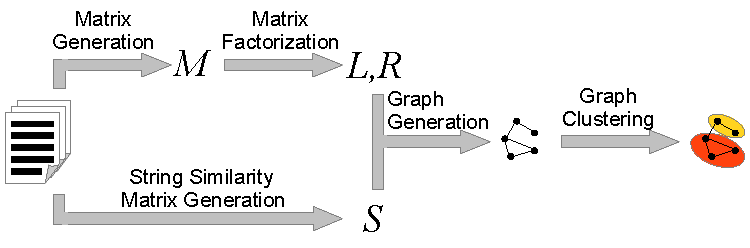
\includegraphics[width=0.9\textwidth]{chapter_three/unstructured_annotation/LD4IE_ISWC_CDCR/cdcr_SystemOverview.pdf}
\caption{The five steps of our approach.}
\label{fig:SystemOverview}
\end{figure}

%\todo[inline]{all: If somebody knows a program with which I can create a better picture than this, please let me know. Axel: Picture is fine}
%\todo[inline]{Micha: Refactor this section. Axel: Done}

\subsection{Matrix Generation}
%\todo[inline]{Micha}
The first step of our approach consists of generating a matrix which describes the context of every named entity mention inside the texts by means of a bag of words.
To this end, the given corpus is preprocessed by tokenizing the documents, removing stop words and indexing the remaining tokens.
In these tokenized documents, the context of a named entity mention is defined as the multiset of tokens inside a window with the size $\pm \sigma$ that is centered on the named entity's tokens.
The contexts are stored in a matrix $M$ containing a row for every named entity mention and a column for every indexed word.
The entries of the matrix are the counts of the words inside the entity mention's context.
As an example, let us consider the sentence 
\begin{ex}
\texttt{Yesterday, VW's CEO presented the new \underline{Golf} in Munich}.
\end{ex}
from which the stopwords \{\texttt{the}, \texttt{in}\} are removed.
For the window size $\sigma = 1$, we get the bag-of-word multiset \{\texttt{new} (1), \texttt{Munich} (1)\} as representation of ``Golf''.
Within the vector space spawned by (\texttt{presented}, \texttt{new}, \texttt{Munich}, \texttt{Germany}), this mention has the vector representation $(0, 1, 1, 0)$.
In the following, we will consider five entity mentions $g_1$, $g_2$, $g_3$, $g_4$ and $g_5$ labelled with the same word ``golf'' as example. 
These entity mentions will be assumed to be represented by the vectors 
$g_1 = (2,2,2,0)$, $g_2 = (1, 0, 0, 1)$, $g_3= (0,0,0,1)$, $g_4=(1, 0, 0, 0)$ and $g_5=(0, 1,1,0)$. 

\subsection{Matrix Factorization}
The matrix $M$ is now a matrix of dimensions $n \times m$ (denoted $M(n,m)$). 
The goal of a matrix factorization is to compute the matrices $L(n, \rho)$ and $R(m, \rho)$ such that $M \approx LR^{\top}$.
We call $\rho \in \mathbb{N} \backslash {0}$ the \emph{rank} of the factorization.
Several approaches have been used to factorize matrices.
Here, we loosely follow the tensor factorization approach presented in~\cite{DBLP:conf/www/NickelTK12}: Given two matrices $L$ and $R$ that are supposed to be the factors of $M$, the overall quadratic error of the approximation is the square Frobenius norm of $E = M - RL^{\top}$, i.e., $||E||_F^2 = ||M - RL^{\top}||_F^2$.
%We can express each entry of the squared Frobenius norm as follows:
%\begin{equation}
%e_{ij}^2 = \left(m_{ij} - \sum\limits_{k = 1}^r r_{ik}l_{jk}\right)^2.
%\end{equation}
%The error is minimal when the first partial derivative of $e_{ij}^2$ becomes 0.
%Thus, we need to minimize the values
%\begin{equation}
%\frac{\partial e_{ij}}{\partial r_{ik}} = -2 e_{ij}l_{jk} 
%\end{equation}
%and
%\begin{equation}
%\frac{\partial e_{ij}}{\partial l_{jk}} = -2 e_{ij}r_{ik}.
%\end{equation}
Previous works have shown that to prevent overfitting, the error function to minimize must be extended.
While several approaches have been suggested to this end, we adopt the error expression given by $||E||_F^2 - \frac{\lambda}{2}(||R||_F^2 + ||L||_F^2)$, where $\lambda \in [0, 1]$ controls how well $L$ and $R$ fit $M$. 
Thus, the error derivatives are as follows:
\begin{equation}
\frac{\partial e_{ij}}{\partial r_{ik}} = -2 e_{ij}l_{jk} + \lambda r_{ik}  
\end{equation}
 and 
\begin{equation}
\frac{\partial e_{ij}}{\partial l_{jk}} = -2 e_{ij}r_{ik} + \lambda l_{jk}.  
\end{equation}
We can now adopt a gradient descent approach to update the matrices $L$ and $R$ and reduce the error they lead to by overwriting each $l_{ik}$ resp $r_{jk}$ as follows:
\begin{equation}
l_{jk} \leftarrow l_{jk} - \alpha \frac{\partial e_{ij}}{\partial l_{jk}} = l_{jk} + \alpha \left(2 \sum\limits_{i=1}^n e_{ij}r_{ik} - \lambda l_{jk} \right)
\end{equation}
and
\begin{equation}
r_{ik} \leftarrow r_{ik} - \alpha \frac{\partial e_{ij}}{\partial r_{ik}} = r_{ik} + \alpha \left(2 \sum\limits_{j=1}^j e_{ij}l_{jk} - \lambda r_{ik} \right).
\end{equation}
We initialize $L$ and $R$ with random entries between 0 and $\max m_{ij}$.
%One problem that has remained unaddressed so far are the initialization of $L$ and $R$ as well as determining the correct settings for the parameters $r$, $\alpha$ and $\lambda$.
For our example, we get
\begin{equation}
M = \left(
\begin{matrix}
 2 & 2 & 2 & 0 \\
 1 & 0 & 0 & 1 \\
 0 & 0 & 0 & 1 \\
 1 & 0 & 0 & 0 \\
 0 & 1 & 1 & 0
\end{matrix} \right).
\end{equation}
For $\rho=2$, our approach computes
\begin{equation}
L = \left(
\begin{matrix}
  1.385 & 1.102 \\
 -0.006 & 0.501  \\
  0.079 & -0.051  \\
 -0.234 & 0.712 \\
  0.933 & -0.168
\end{matrix} \right)
\quad \text{and} \quad R = \left(
\begin{matrix}
 0.331 & 1.406 \\
 1.059 & 0.446 \\
 1.118 & 0.363 \\
 0.062 & 0.066
\end{matrix} \right).
\end{equation}
The intuition behind our approach is that $L$ is a better and compressed description of the entity mentions than $M$.
Hence, we now use $L$ in combination with a string similarity function to compute the similarity of entity mentions.

\subsection{String Similarity Matrix}
The string similarity matrix $S$ is an optional feature of our approach.
Each entry $s_{ij}$ of $S$ describes the similarity between the label of the $i$th and the $j$th entity in our input corpus.
Assuming a symmetric string similarity function such as the 3-gram similarity (which we use in our experiments), 
we also get a symmetric string similarity matrix $S$.
%Compute string similarity matrix $S$ using $n$-gram similarity with $n=3$.
We assume $s_{ij} = 1$ if no string similarity is specified.
$s_{ij} = 1$ also holds for our example, as all mentions are labelled with ``golf''.

\subsection{Graph Generation}
The aim of the graph generation is to generate a similarity graph $G = (V, E, w)$ that will allow detecting mentions of the same real-world object through clustering.
The set of vertices of $V$ is the set of entity mentions in our corpus.
We define the weight function $w: V \times V \rightarrow [0, 1]$ as $w(v_i, v_j) = s_{ij} \times \frac{l_{(i,\cdot)} \cdot l_{(j,\cdot)}}{||l_{(i,\cdot)}|| \times ||l_{(j,\cdot)}||}$, where $l_{(i,\cdot)}$ is the $i$th row-vector of $L$ and stands for the latent description of the $i$th entity mention in the corpus.
Given that many graph clustering approaches are polynomial in the number of edges, we can control $|E|$ by only setting an edge between $v_i$ and $v_j$ if $w(v_i, v_j) \geq \theta \in [0, 1]$.
%Remove edges with $g_{ij} \le \theta$ (=threshold)
For $\theta = 0.3$ and $\rho=2$ we end up with the graph displayed in Figure~\ref{fig:latent}. 
As comparison, Figure~\ref{fig:original} shows the graph obtained with by setting $L = M$, i.e., generating $G$ without using latent features.

\begin{figure}
\centering
\usetikzlibrary{arrows}

\begin{tikzpicture}[auto,node distance=2cm,
  thick,main node/.style={circle,fill=blue!20,draw,font=\sffamily\bfseries}]

  \node[main node] (1) {$g_1$};
  \node[main node] (2) [below left of=1] {$g_2$};
  \node[main node] (3) [above left of=1] {$g_3$};
  \node[main node] (4) [above right of=1] {$g_4$};
  \node[main node] (5) [below right of=1] {$g_5$};

  \path[every node/.style={font=\sffamily\small}]
    (1) edge node [left] {0.61} (2)
        edge node [left] {0.31} (3)
        edge node [left] {0.34} (4)
        edge node [left] {0.61} (5)
    (3) edge node [below] {0.95} (4)
    (2) edge node [above] {0.92} (5);    
\end{tikzpicture}
\caption{Graph generated using $\rho=2$}
\label{fig:latent}
\end{figure}

\begin{figure}
\centering
\usetikzlibrary{arrows}
\begin{tikzpicture}[auto,node distance=2cm,
  thick,main node/.style={circle,fill=blue!20,draw,font=\sffamily\bfseries}]

  \node[main node] (1) {$g_1$};
  \node[main node] (2) [below left of=1] {$g_2$};
  \node[main node] (3) [above left of=1] {$g_3$};
  \node[main node] (4) [below right of=1] {$g_4$};
  \node[main node] (5) [above right of=1] {$g_5$};

  \path[every node/.style={font=\sffamily\small}]
    (1) edge node [left] {0.41} (2)
        edge node [left] {0.58} (3)
        edge node [left] {0.82} (5)
    (2) edge node [left] {0.71} (3)
    (2) edge node [above] {0.71} (4);    
\end{tikzpicture}
\caption{Graph generated using $M$ instead of $L$}
\label{fig:original}
\end{figure}

\subsection{Graph Clustering}
%\todo[inline]{Axel}
We now cluster the graph $G$ to detect mentions that stand for the same real-world object.
Our approach can rely on any graph clustering approach.
In our current implementation, we rely on the BorderFlow algorithm~\cite{DBLP:conf/cicling/NgomoS09} because it is parameter-free.
BorderFlow regards any set $C \subseteq V$ as having a \emph{border} $b(C) = \{v \in C: \exists u \in V \backslash C \mbox{ with } (v, u) \in E\}$.
The \emph{flow} $\Omega(C_1, C_2)$ between two sets $C_1 \subseteq V$ and  $C_2 \subseteq V$ is defined as $\Omega(C_1, C_2) = \sum\limits_{v \in C_1, u \in C_2} w(v, u)$.
Based on these definitions, BorderFlow implements a local graph clustering paradigm by mapping each node $v \in V$ to the set of nodes $C \subseteq V$ that is such that $v \in C$ and $C$ is a node-maximal set w.r.t. the function 
\begin{equation}
bf(C) = \frac{\Omega(b(C), C)}{\Omega(b(C), V \backslash C)}.
\end{equation}
While finding the optimal $C$ for each $v$ can be very time-consuming, the heuristic presented in~\cite{DBLP:bibsonomy_NGO10b} allows determining an approximation of $C$ in an efficient manner.
We employ this heuristic herein.

Now, the result of BorderFlow is not a partitioning of the graph.
Rather, clusters may overlap.
We thus employ a \emph{hardening} approach to generate a partitioning of the input graph.
To this end, each node $v\in V$ which belongs to two different clusters $C_1$ and $C_2$ is assigned to $C_1$ iff
\begin{equation}
bf(C_1 \cup \{v\}) + bf(C_2 \backslash \{v\}) \geq bf(C_2 \cup \{v\}) + bf(C_1 \backslash \{v\}).
\end{equation}
In all other cases, $v$ is assigned to $C_2$.
We call this form of hardening \emph{flow maximization}.
Other forms of hardening can be conceived of, e.g., minimizing the number of unions operations that need to be carried out to achieve a partitioning of the graph (\emph{set-based}).

For our example, we get the clusters $\{g_1, g_5\}$ and $\{g_2, g_3, g_4\}$ for $\rho=2$ when using BorderFlow with any partitioning approach.
If we replace $L$ with $M$, we get the clusters  $\{g_1\}$, $\{g_2, g_4\}$ and $\{g_3, g_5\}$.
This result on toy data already suggests that matrix factorization leads to results that differ from those gathered when using raw data.
In the subsequent section, we show empirically that using $L$ to generate $G$ leads to more accurate results than using $M$ to generate $G$.

\section{Evaluation}

\label{cha314:sec:evalval}

\subsection{Experimental Setup}

\subsubsection{Goals}
The goal of our experiments was two-fold. First, we wanted to measure the effect of the different parameters on our approach.
Moreover, we wanted to know whether the factorization outperforms a comparable baseline.
To achieve the first goal of our experiments, we conducted experiments where we varied the rank $\rho$ as well as the window size $\sigma$ while keeping all other parameters fixed.
We addressed the second goal by creating a baseline as follows: We ran our pipeline as described in the sections above with the sole difference that (1) we did not carry out a factorization and (2) we use $M$ instead of $L$ as input for the graph clustering. All other steps (matrix generation, graph generation, graph clustering) remained unchanged.
The similarity threshold for the graph generation is set to $\theta=0.1$ for all our experiments.

\subsubsection{Datasets}
We use the three corpora of the $\mbox{N}^3$ collection~\cite{n3} in our experiments.
%\todo[inline]{Actually here could be an error, which leads to very high f-measure}
%Each corpus was annotated manually, i.e., each entity mention was mapped to an URI from DBpedia~\cite{lehmann2014dbpedia} or a URI from the \url{http://aksw.org/} namespace if no corresponding resource could be found in DBpedia.
%
\begin{itemize}
\item The \textbf{News-100} corpus comprises 100 German news articles from \url{news.de}.
Each of these articles contains the German word ``Golf''---a homonym that has three different meanings inside these documents.
The word could mean (a) a gulf, e.g., the Mexican gulf, (b) the ball sport or (c) a compact car of the German manufacturer Volkswagen.
This is clearly the most difficult dataset, as many resources share exactly the same name but have different meanings. 
\item The \textbf{Reuters-128} corpus contains 128 English economy news articles from the Reuters news agency.
The documents in this dataset are smaller than the ones from the News-100 corpus providing a shallow context.
\item The third corpus, \textbf{RSS-500}, contains 500 documents each with only one sentence.
The sentences were randomly chosen from a larger amount of RSS news feeds, as described in~\cite{GER+13}.
Every sentence contains exactly two named entities.
\end{itemize}
Table~\ref{tab:corpusStats} provides further detailed information about the corpora.
On average, each named entity occurs nearly 5 times in the News-100 corpus.
Within the Reuters-128 corpus nearly two mentions per named entity exist on average while in the RSS-500 corpus only every tenth entity is mentioned more than once.

%\todo[inline]{Micha: describe N${}^{3}$}

\begin{table}[thb]
    \caption{Features of the corpora}
    \begin{tabular}{lp{0.7cm}rp{0.3cm}p{0.7cm}rp{0.2cm}p{0.6cm}rp{0.3cm}}
    \toprule
     & \multicolumn{3}{c}{\textbf{News-100}} & \multicolumn{3}{c}{\textbf{Reuters-128}} & \multicolumn{3}{c}{\textbf{RSS-500}} \\
    \midrule
    Documents && 100 &&& 128 &&& 500 &\\
	Tokens && 48199 &&& 33413 &&& 31640 &\\
	Entities && 362 &&& 444 &&& 849 &\\
    Mentions && 1655 &&& 880 &&& 1000 &\\
	\bottomrule
	\end{tabular}
	\centering
	\label{tab:corpusStats}
\end{table}

\subsection{Results}

\subsubsection{Influence of rank}
In our first series of experiments, we fixed the window size to 4 and measured the influence of the rank $\rho$ on the precision, recall and F-measure. 
The left side of Figure~\ref{fig:results} shows the results of our experiments on the three datasets.
Most importantly, our results show that we outperform the baseline in most settings.
We achieve the best increase of performance on the RSS-500 corpus, where we achieve a 20.5\% increase in F-measure over the baseline.
This result suggest that our approach does not tend to overgeneralize through the compression on information that is carried out during the factorization.
Instead, our results suggest that we get rid of a significant amount of noise while factorizing.
Our results on the other two datasets show that we also achieve a better F-measure (increases of 18.2\% on Reuters-128 and 6.3\% on News-100, see Table~\ref{tab:improvements}). 
An analysis of the results reveals that this increase is mostly due to the significant increase in precision that we achieve in most settings.
On the other hand, our recall is rarely ever worse than that of the baseline.
This suggests that BorderFlow tends to generate smaller clusters with factorization than when the baseline approach is used.
We measure the statistical significance of our results using a Wilcoxon signed rank-test with 95\% confidence.
Our results are significant in all cases.%\todo[inline]{Check this}

\subsubsection{Influence of window size}
In this experiment, we set the rank to 100 for all experiments and measured the effect of the window size on the overall F-measure of our approach.
The right half of Figure~\ref{fig:results} shows the results of this series of experiments on the three datasets.
Overall, our results suggest that for this rank, the window size does not have a major influence on the F-measure. 
This also seems to hold for other ranks.
Interestingly, a small window size seems to lead to good results in most cases when we use the factorization. While we assume that this might be due to the factorization being able to convert the two words within the window to their latent features    
This result indicates that small window sizes suffice for our approach to achieve better F-measures than the baseline on the CDCR problem.
This might mean that a small set of words is already sufficient to disambiguate resources across different documents.

\begin{figure}[t!]
\centering
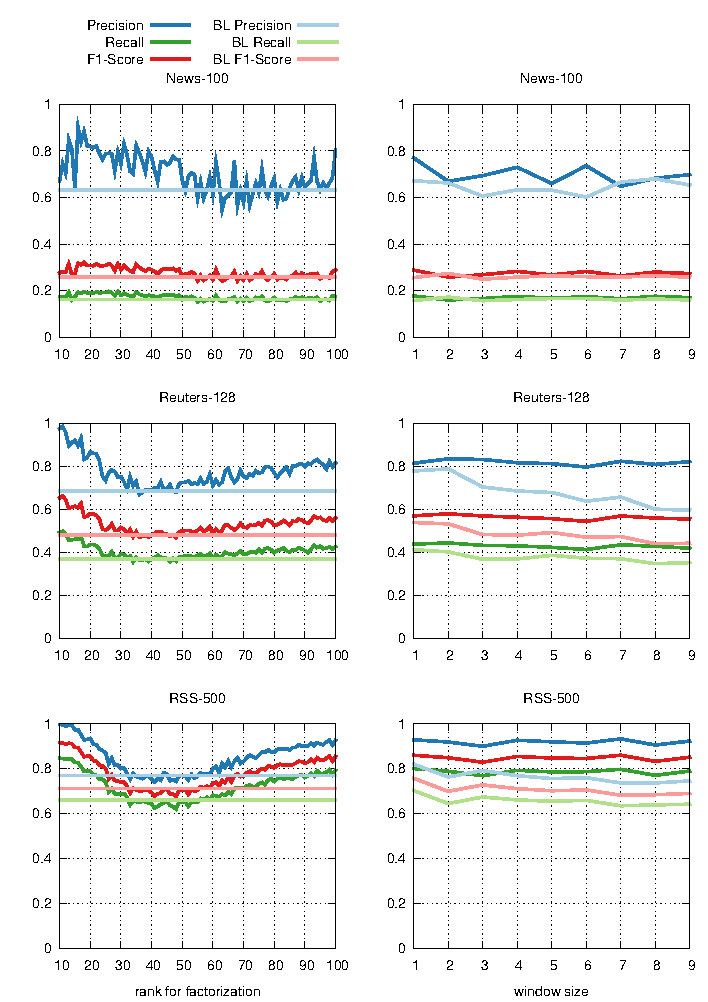
\includegraphics[width = \textwidth]{chapter_three/unstructured_annotation/LD4IE_ISWC_CDCR/cdcr_results_Flow.pdf}
\caption{Precision, recall and F1-score of our approach with different ranks (left) and different window sizes (right) compared to the baseline (BL). The diagrams show the results for the flow maximization hardening.}
\label{fig:results}
\end{figure}
\afterpage{\clearpage}

\subsection{Effect of hardening}
In all results presented above, we used a hardening based on the borderflow ratio.
We also implemented the set-based hardening mentioned above and compared the results we achieve with this hardening.
Overall, our results suggest that the borderflow-maximization approach that we used for hardening generates the best results both for the baseline and our approach. 
Moreover, we outperform the baseline independently from the hardening used.

\begin{table}[htb]
    \caption{Best improvements in F-measure of our approach (OA) over the baseline (BL)}
    \begin{tabular}{lp{1cm}p{0.25cm}rp{1cm}p{0.25cm}rp{1cm}p{0.25cm}rp{1cm}p{0.25cm}r}
    \toprule
     && \multicolumn{5}{c}{\textbf{Flow Maximization}} && \multicolumn{5}{c}{\textbf{Set-Based}} \\
     && \multicolumn{2}{c}{BL} && \multicolumn{2}{c}{OA} && \multicolumn{2}{c}{BL} && \multicolumn{2}{c}{OA} \\
    \midrule
    News-100        &&& 25.86  &&& \textbf{32.21} &&& 23.87  &&& \textbf{28.81} \\
	Reuters-128     &&& 47.89  &&& \textbf{66.16} &&& 47.00  &&& \textbf{56.65} \\
	RSS-500         &&& 71.11  &&& \textbf{91.62} &&& 69.57  &&& \textbf{85.71} \\
	\bottomrule
	\end{tabular}
	\centering
	\label{tab:improvements}
\end{table}

%\subsection{Scalability}\todo[inline]{Please fill gaps}
%One last question that we addressed is the scalability of our approach.
%We ran our experiments on a Debian machine (Intel Xeon 3.10GHz, 8GB RAM).
%On average, the baseline experiments ran 22.7s for News-100, ??? for Reuters-128 and ??? for RSS-500.
%In contrast, the experiments with factorization ran ??? for News-100, ??? for Reuters-128 and ??? for RSS-500.
%These results suggest that our approach scales when and does not produce a significant overhead in runtime while generating significantly better results.

\subsubsection{Discussion}
Overall, our initial results suggest that we indeed outperform the proposed baseline by using matrix factorization (see Table~\ref{tab:improvements}).
Still, many questions do remain open.
The most important question that we did not address is when should a high rank be used?
First, in our experiments, $\rho=10$ was sufficient across all datasets to outperform the baseline. 
To the best of our knowledge, finding the optimal rank for a factorization problem is an open question.
Nevertheless, we think that the answer to this question lies in the amount of information contained in the corpus.
The higher the information density of a corpus, the higher the rank required to characterize entity adequately.
A second question that remains unanswered is whether we can improve the results of the factorization by considering known resources in the dataset.
We will address this question in future work by disambiguating using a combination of textual information and Linked Data.
%\todo[inline]{Micha: Refactor the current figure. It doesn't look really nice.}

%\subsubsection{Runtime}
%We also measured the runtime of our approach across all experiments. Our results suggest that our approach can actually lead to significantly smaller runtimes. However, the settings in which we achieve the best runtimes correspond to settings in which the overall runtime of our approach is comparable to that of the baseline. This is obviously a satisfactory results as it means that we can achieve better F-measure without requiring significantly higher processing times.

\section{Conclusion}
\label{cha314:sec:conclusion}
In this paper, we presented a CDCR approach based on latent features.
We showed that our approach can outperform our baseline by more than 10\% F-measure.
%Moreover, we showed that our approach scales well and can thus be used on large datasets.
We will use our approach to complement the entity linking framework~\cite{agdistis_iswc} when it is used in batch mode, i.e., over a document corpus at once.
Moreover, we will develop means to detect an appropriate rank for factorization.
To this end, we plan to use the derivative of the mean squared error $||M - LR^{\top}||^2_F$.
Finally, we will develop a deterministic approach to initialize $L$ and $R$. 
Preliminary results on random matrices show that we can already reduce the initial value of $||E||^2_F$ by more approximately 40\%, leading to a significantly faster convergence of the factorization.



%\end{document}


\begin{comment}
\begin{table}[htb]
    \caption{Best improvements of our approach over the baseline}
    \begin{tabular}{lp{0.5cm}cp{0.5cm}cp{0.5cm}c}
    \toprule
     && \multicolumn{1}{c}{\textbf{Rank}} && \multicolumn{1}{c}{\textbf{Baseline (F1)}} && \multicolumn{1}{c}{\textbf{Our approach (F1)}} \\
    \midrule
    News-100        && 11   && 56.78  && 62.99 \\
	Reuters-128     && 91   && 68.23  && 71.63 \\
	RSS-500         && 97   && 79.31  && 88.40 \\
	\bottomrule
	\end{tabular}
	\centering
	\label{tab:improvements}
\end{table}
\end{comment}

\begin{comment}
\subsection{Initialization of $L$ and $R$}
In most approaches, the matrices $L$ and $R$ are initialized by using random values.
While this approach still leads to converging results in practical applications, it is unsatisfactory as the results of the factorization may be different across different initializations.
We address the initialization problem by using a correlation-based approach.
The intuition behind our approach is that the latent features describe a space whose basic vectors stand for weakly correlated dimensions. 
We can thus initialize the matrices $L$ (and analogously the matrix $R$) by detecting the rows (resp. columns) that display the smallest correlation to other rows and using those as our initialization for $L$.
We go about implementing this intuition as follows: Let 
\begin{equation}
B = M \times M^\top \mbox{ and } A = \frac{B}{\max\limits_{i, j} b_{ij}}.
\end{equation}
The matrix $A$ encompasses how correlated the rows in $M$ are.
We assign each row $a_{i}$ a weight $w_i = \sum_{j=1}{n} a_{ij}$.
The weight $w_i$ tells us how correlated $a_i$ is to $a_1 \ldots a_n$.
We now sort the rows according to their weights in ascending order and select the r rows with the smallest weight.
These rows are then used to initialize $L$, ergo $l_1 = a_k$ with $\forall i \neq k, w_i \geq w_k$.  

The matrix $R$ can be initialized analogously by setting 
\begin{equation}
B = M^\top \times M \mbox{ and } A = \frac{B}{\max\limits_{i, j} b_{ij}}.
\end{equation}
\todo{Add example}

\begin{itemize}
\item use FOX to do NER over several documents \todo{No need for FOX in the experiments. Simply use the benchmarks directly.} 
\todo{Now it is implemented and getting back to the original work would be cumbersome.} 
\item describe an entity by its neighbors, i.e., window size and latent features
\item use cosine similarity as a baseline
\item cluster those entities across documents using Axels framework
\item named entities are the same resources if they end up in the same cluster...\todo[inline]{RU: I fear the noise hear when number of clusters is too low}
\item formulate good URIs for them, see http://www.w3.org/TR/cooluris/

\end{itemize}

LR^T = 

  5,103 1,896 -0,712 1,555
  3,412 1,274 -0,450 1,085
  1,540 1,040  1,780 3,949
  1,169 0,799  1,394 3,073
 -0,438 0,543  3,076 5,125
\end{comment}



\chapter{GERBIL -- General Entity Annotator Benchmarking Framework}

\graffito{
This chapter introduces GERBIL--a framework for benchmarking semantic annotation systems with the ultimate goal to provide stable, citable URIs for comparable experiments. 
The author of this thesis is the main author of~\cite{gerbil_demo_2015,GERBIL} and co-author of~\cite{gerbil_dev_2015} which are peer-reviewed publications.
He co-implemented  and co-evaluated GERBIL together with Michael Röder.
GERBIL won the Best Demo Award 2015 at the Extended Semantic Web Conference.
}
\label{cha:gerbil}
The implementation of the original vision behind the Semantic Web demands the development of approaches and frameworks for the seamless extraction of structured data from text. 
While manifold annotation tools have been developed over the last years to address (some of) the subtasks related to the extraction of structured data from unstructured data \cite{TagMe2,AIDA,spotlight,milne2008learning,babelfy,piccinno2014tagme,rizzo2014,Steinmetz2013,agdistis_iswc}, the provision of comparable results for these tools remains a tedious problem. The issue of  comparability of results is not to be regarded as being intrinsic to the annotation task. Indeed, it is now well established that scientists spend between 60\% and 80\% of their time preparing data for experiments \cite{GIL2014,jermyn1999preparing,peng2011reproducible}. Data preparation being such a tedious problem in the annotation domain is mostly due to the different formats of the gold standards as well as the different data representations across reference datasets.
%\todo[inline]{AnBo: --change-- different formatting of the textual data in reference datasets --to-- different data representations in reference datasets. Axel:Done}
These restrictions have led to authors evaluating their approaches on datasets (1) that are available to them and (2) for which writing a parser as well as of an evaluation tool can be carried out with reasonable effort.
%\todo[inline]{AnBo: easy sounds like an affront, suggestion: is easy --to-- can be implemented within reasonable effort. Axel: Done.} 
In addition, a large number of quality measures have been developed and used actively across the annotation research community to evaluate the same task, leading to the results across publications on the same topics not being easily comparable. For example, while some authors publish macro-F-measures and simply call them F-measures, others publish micro-F-measures for the same purpose, leading to significant discrepancies across the scores. The same holds for the evaluation of how well entities match. Indeed, partial matches and complete matches have been used in previous evaluations of annotation tools \cite{cornolti,FOX}. This heterogeneous landscape of tools, datasets and measures leads to a poor repeatability of experiments, which makes the evaluation of the real performance of novel approaches against the state of the art rather difficult.

The insights above have led to a movement towards the creation of frameworks to ease the evaluation of solutions that address the same annotation problem~\cite{ERD2014,cornolti}. 
We present GERBIL -- a general entity annotator benchmark --, a community-driven effort to enable the continuous evaluation of annotation tools. GERBIL is an open-source and extensible framework that allows evaluating tools against (currently) \overallGERBILannotators different annotators on \overalldatasets different datasets within 6 different experiment types.\footnote{Numbers are taken from the 2015 publication~\cite{GERBIL}. Current numbers can be found in Section~\ref{sec:currentNumbersForGERBIL}}. 
%At this point in time, GERBIL integrates . Moreover, \overallNrOfMatchingTypes matching types are provided. 
By integrating such a large number of datasets, experiment types and frameworks, GERBIL allows users to evaluate their tools against other semantic entity annotation systems (short: entity annotation systems) by using exactly the same setting, leading to fair comparisons based on exactly the same measures. 
While the evaluation core of GERBIL is based on the BAT-framework \cite{cornolti}, our approach goes beyond the state of the art in several respects:
\begin{itemize}
\item GERBIL provides \emph{persistent URLs} for experimental settings. Hence, by using GERBIL for experiments, tool developers can ensure that the settings for their experiments (measures, datasets, versions of the reference frameworks, etc.) can be reconstructed in a  unique manner in future works. 
\item Through experiment URLs, GERBIL also addresses the problem of \emph{archiving} experimental results and allows end users to gather all pieces of information required to choose annotation frameworks for practical applications.
\item GERBIL aims to be a \emph{central repository for annotation results} without being a central point of failure: While we make experiment URLs available, we also provide users directly with their results to ensure that they use them locally without having to rely on GERBIL.
\item The results of GERBIL are published in a \emph{machine-readable format}. In particular, our use of DataID~\cite{dataID} and DataCube~\cite{datacube} to denote tools and datasets ensures that results can be easily combined and queried (for example to study the evolution of the performance of frameworks) while the exact configuration of the experiments remains uniquely reconstructable. By these means, we also tackle the problem of \emph{reproducibility}. 
\item Through the provision of results on different datasets of different types and the provision of results on a simple user interface, GERBIL also provides means to quickly gain an overview of the current performance of annotation tools, thus providing (1) developers with insights pertaining to the type of data on which their accuracy needs improvement and (2) end users with insights allowing them to choose the right tool for the tasks at hand.
\item With GERBIL we introduce the notion of knowledge base-agnostic benchmarking of entity annotation systems through generalized experiment types. By these means, we allow benchmarking tools against reference datasets from any domain grounded in any reference knowledge base. 
\end{itemize}


To ensure that the GERBIL framework is useful to both end users and tool developers, its architecture and interface were designed with the following principles in mind:

\begin{itemize}
\item \textbf{Easy integration of annotators}: We provide a wrapping interface that allows annotators to be evaluated via their REST interface. In particular, we integrated \numberOfadditionalAnnotators additional annotators not evaluated against each other in previous works (e.g., \cite{cornolti}).  
\item \textbf{Easy integration of datasets}: We also provide means to gather datasets for evaluation directly from data services such as DataHub.\footnote{\url{http://datahub.io}} In particular, we added \numberOfadditionalDatasets new datasets to GERBIL.
\item \textbf{Easy addition of new measures}: The evaluation measures used by GERBIL are implemented as interfaces. Thus, the framework can be easily extended with novel measures devised by the annotation community.
\item \textbf{Extensibility}: GERBIL is provided as an open-source platform that can be extended by members of the community both to new tasks and different purposes.
\item \textbf{Diagnostics}: The interface of the tool was designed to provide developers with means to easily detect aspects in which their tool(s) need(s) to be improved. 
\item \textbf{Portability of results}: We generate human- and machine-readable results to ensure maximum usefulness and portability of the results generated by our framework. 
\end{itemize}


The rest of this chapter presents and evaluates GERBIL. 
%We begin by giving an overview of related work.
First, we present the GERBIL framework.
Especially, we focus in particular on how annotators and datasets can be added to GERBIL and give a short overview of the annotators and tools that are currently included in the framework. 
We then present an evaluation of the framework that aims to quantify the effort necessary to include novel annotators and datasets to the framework. 
We conclude with a discussion of the current state of GERBIL and a presentation of future work. 
More information can be found at our project webpage \url{http://gerbil.aksw.org} and at the open source code repository page \url{https://github.com/AKSW/gerbil}.
The online version of GERBIL can be accessed at \url{http://gerbil.aksw.org/gerbil}.


\section{The GERBIL Framework}
\label{sec:architecture}
\begin{figure*}[tb]
\centering
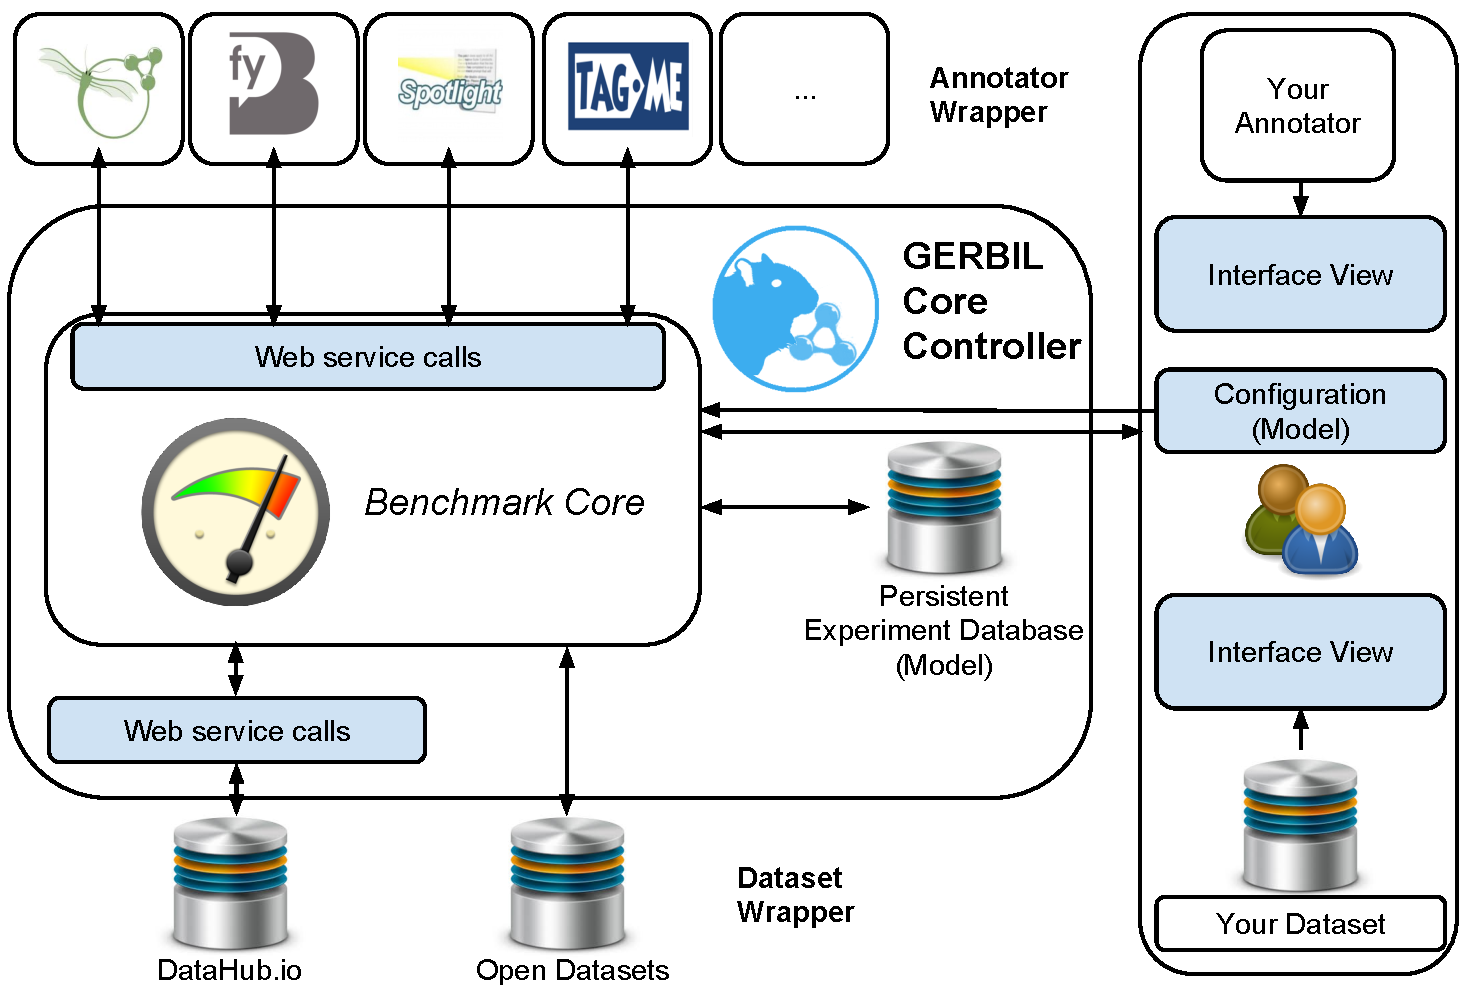
\includegraphics[width=\linewidth]{part_02/benchmarking/WWW_GERBIL/GERBIL_new_architectur}
\caption{Overview of GERBIL's abstract architecture. Interfaces to users and providers of datasets and annotators are marked in blue.
%\todo[inline]{AnBo: Should the arrows/calls triggered from the core \emph{to}\ the datasets?}
}
\label{fig:architecture}
\end{figure*}

%Publishing, reproducing and archiving entity annotation results is a near-impossible endeavour.
%Finding and reusing datasets for comprehensive benchmarks involves often a trem\-endous amount of addition work.

\paragraph{Architecture Overview}
GERBIL abides by a service-oriented architecture driven by the architectural pattern of model-view-controller (see Figure~\ref{fig:architecture}).
Entity annotation systems, datasets and configurations like experiment type, matching or metric are implemented as controller interfaces easily pluggable to the core controller. 
The output of experiments as well as descriptions of the various components are stored in a serverless database for fast deployment. % reachable from each controller. 
Finally, the view component displays configuration options respectively renders experiment results delivered by the main controller communication with the diverse interfaces and the database.

%\todo[inline]{AnBo: I have doubts regarding the buzzwords here. 1) A SOA needs a service repository providing callable interfaces to services but do not wrap the service. I am not sure what the actual implementation status is. Maybe we should take over the wording of our SEMANTiCS paper: oriented at the principles of service-oriented architectures. But maybe it is more closely to a plugin-architecture?
%2) Implementing a MVC pattern with distributed services is very complicated. Maybe a MVP pattern is a good description of the actual implementation?}
%\todo[inline]{How does GERBIL work internally? Short description of architecture needed}



% of fine grained measures to be able to cover a wide variety of experiments using diverse NER and NED approaches.
%GERBILs core is based on the endeavour of Cornolti et al.'s BAT-Framework~\cite{cornolti} for comparing entity annotation systems. 

%\todo[inline]{(Andrea) We should add a table/image/example to clarify the different setups, even if some of them do not properly belong to the NED/EL/NEL/NER categories such as C2W, Sc2W and Rc2W which do not require the actual mention/entity mapping. Moreover, Sa2W and A2W can be seen as the same task assuming that the score for A2W systems is always equal to 1. (Ricardo): I agree with the last sentence. But that is how it is given in Cornoltis work. Furthermore, I would like to add a table mapping the approaches to categories. What do you think? And maybe add examples to the table below. (Andrea): which kind of categories? I don't think that examples for all the setups are really needed there should be only a single general example to make clear what EL is}
%postponed to M2 paper


\subsection{Features}
\label{sec:definitions}
%\todo[inline]{@Marco, Paolo/@Ricardo: please proof read this subsection}

%\begin{table*}[th]
\centering
\begin{tabular}{@{}p{3cm}p{2cm}p{3cm}p{7cm}@{}}
\toprule
Problem & Input & Output & Description \\ \midrule


Disambiguate to Wikipedia (D2KB) &
Text, Set of mentions &
Set of relevant annotations &
Assign to each input mention its pertinent entity (possibly null) \\ \midrule

Annotate to Wikipedia (A2KB) &
Text &
Set of relevant annotations &
Identify the relevant mentions in the input text and assign to each of them the pertinent entities \\ \midrule

Scored-annotate to Wikipedia (Sa2KB) &
Text &
Set of relevant and scored annotations &
As A2W, but here each annotation is assigned a score representing the likelihood that the annotation is correct \\ \midrule

Concepts to Wikipedia (C2KB) &
Text &
Set of relevant tags &
Tags are taken as the set of relevant entities that are mentioned in the input text \\ \midrule

Scored concepts to Wikipedia (Sc2KB) &
Text &
Set of relevant and scored tags &
As C2W, but here each tag is assigned a score representing the likelihood that the annotation is correct \\ \midrule

Ranked-concepts to Wikipedia (Rc2KB) &
Text &
Ranked list of relevant tags &
Identify the entities mentioned in a text and rank them in terms of their relevance for the topics dealt with in the
input text\\ \midrule

Classification/Typing to Wikipedia (T2KB) &
 &
 &
\\ \midrule

Entity Salience (ES2KB) &
  &
  &
\\\midrule

Entity Annotation/Detection (A) &
  &
  &
\\
\midrule
Word Sense Disambiguation (WSD) &
  &
  &
\\
\midrule
Relation Extraction (input text, predicate output: triple (BOA?) &
  &
  &\\
\bottomrule
\end{tabular}
\caption{Overview of the different task types.}
\label{tab:tasktypes}
\end{table*}

%\todo[inline]{add a table of mappings from tools to tasks}
%\todo[inline]{@Ricardo,Giuseppe,Micha, Axel: Discuss matchings (esp. TAC-KBP }
%postponed to M2
%\todo[inline]{(Ricardo) we need to discuss how to handle NIL entities while linking step, maybe consider measures from http://jhoff.de/wp-content/papercite-data/pdf/hoffart-2014hp.pdf. \\(Giuseppe) Whenever you refer to NIL then you are touching the TAC KBP EL/EDL effort somehow. There is already a consistent and mature body of work on that. I also encourage you to take a look at http://nlp.cs.rpi.edu/kbp/2014/KBP2014EL\_V1.1.pdf. The metrics proposed in TAC KBP already measure the effect of NIL links.}
%postponed to M2
%Here, we want to point to two import task types, i.e., D2W - disambiguation to Wikipedia which determines for each mention in a given set of mentions its pertinent entity~\cite{Cucerzan07} - and A2W - annotation to Wikipedia  which determines for a given unstructured text a set of relevant entities~\cite{milne2008learning}.
%'These problems can be casted in two main classes: the first consists of three problems which address the identification of (possibly scored) annotations, and thus the identification of mention-entity pairs; the second consists of three further problems that involve finding tags (possibly scored or ranked), thus accounting only for the entities.'
%For a detailed list of problems and their definition please have a look at the article itself~\cite{cornolti}.

Experiments run in our framework can be configured in several manners. In the following, we present some of the most important parameters of experiments available in GERBIL. 

\paragraph{Experiment types}
An experiment type defines the way used to solve a certain problem when extracting information.
Cornolti et al.'s~\cite{cornolti} BAT-framework offers six different experiment types, namely (scored) annotation (S/A2KB), disambiguation (D2KB) -- also known as \ac{EL} --, (scored respectively ranked) concept annotation (S/R/C2KB) of texts. 
In~\cite{rizzo2014}, the authors propose two types of experiments, focusing on highlighting the strengths and weaknesses of the analyzed systems.
Thereby, performing \textit{i)} entity recognition, i.e., the detection of the exact match of the pair entity mention and type (e.g., detecting the mention \textit{Barack Obama} and typing it as a \textit{Person}), and \textit{ii)} entity linking, where an exact match of the mention is given and the associated DBpedia URI has to be linked (e.g., locating a resource in DBpedia which describes the mention \textit{Barack Obama}).
This work differs from the previous one for experimenting in entity recognition, and on annotating entities to a \ac{RDF} \ac{KB}.


% (Giuseppe)
%the flow I can get from here is: 
% - people worked on annotating (datasets, knowloedge bases): link or NIL
% - people worked on typing: fine grained (WEKEX, ACE,...) or coarse grained type (CoNLL: per,loc,org,...)
% - TAC KBP combines the two things, but it keeps the tasks in the simple form, i.e. typing only to a coarse grained schema (GPE, per, org) and using a sort-of knowldge base (their own creation of a set of wikipedia resource)
% next: 
% * going further and covering these issues (schemas, links)
% * domain adaptation analysis (Microposts2014 is about microposts, CoNLL is about newswire, etc etc)  
% (Ricardo)
% I guess, we should discuss next steps later, like after the deadline of WWW
% (Giuseppe) oki. But if we mention above the NERD efforts on experimenting NER, then we should claim something similar for GERBIL. Otherwise it's better removing that sentence

GERBIL reuses the six experiments provided by the BAT-framework and extends them by the idea to not only link to Wikipedia but to any knowledge base $K$.
%Thereby, we extend the idea of the before mentioned frameworks by introducing the concept of knowledge base-agnostic benchmarks.
%\todo[inline]{The following sentence does not make sense to me}
%That is, datasets and annotators are aware of their underlying knowledge bases, e.g., Wikipedia, DBpedia, Babelnet etc..
One major formal update of the measures in GERBIL is that in addition to implementing experiment types from previous frameworks, it also measures the influence of NIL annotations, i.e., the linking of entities that are recognized as such but cannot be linked to any resource from the reference knowledge base $K$. For example, the string \texttt{Ricardo Usbeck} can be recognized as a person name by several tools but cannot be linked to Wikipedia/DBpedia, as Ricardo does not have a URI in these reference datasets. 
Our framework extends the experiments types of~\cite{cornolti} as follows: Let $m=(s,l,d,c) \in M$ denote an entity mention in document $d \in D$ with start position $s$, length $l$ and confidence score $c \in [0,1]$.
%that links to either a resource from the resource knowledge base $K$ or a global NIL entity if the entity mentioned is not in $K$. 
Note that some frameworks might not return (1) a position $s$ or a length $l$ for a mention, in which case we set $s=0$ and $l=0$; (2) a score $c$, in which case we set $c=1$.
%(Giuseppe) wikipedia is not a knowledge base. A knowledge base is a representation of the word for computing machinery, hence it has to be semantically structured. According to this definition, DBpedia is. Wikipedia is an encyclopedic resource, or simply a dataset
%\todo[inline]{AnBo@Ricardo: There is a problem with the definition of $m$, either it is $m=(s,l,d)$ without the score, or it has to be $m=(s,l,d,c,e)$ referring the resource e (that might NIL) mentioned in the description and needed for the score $c$. Note (Axel): The entity is given by a different function actually. Here, the tool only finds a mention (NER). NED occurs later :). Note (AnBo): But what expresses $c$ in this case?: Note (Axel): That's the confidence score for the mention.
%You are absolutely right. Just fixed it. It was simply incorrect. The mention must not link to an entity.
%(AnBo: perfect! issue closed.)
%}
%\todo[inline]{@axel,micha: discuss the below
%Old text: All the approaches mentioned in the last paragraphs work on Wikipedia page URIs or ids. 
%Since the introduction of DBpedia in 2007, new semantic approaches have been published based on unique DBpedia entity URIs instead of Wikipedia URIs. 
%Due to the bijective mapping, also older approaches can be used in GERBIL, which is more keen on Semantic Web technologies.
%}

%\todo[inline]{The following does not make any sense to a non-informed reader. The variables are simply not defined and used (see below). Stick to the formal definition of a mention above, which is incomplete, as it does not take $d$ into consideration.}
We implement six types of experiments:
\begin{enumerate}
\item \textbf{D2KB}: The goal of this experiment type is to map a set of \emph{given} entities mentions (i.e., a subset $\mu \subseteq M$) to entities from a given \ac{KB} or to NIL. Formally, this is equivalent to finding a mapping $a: \mu \rightarrow K \cup \{NIL\}$. In the classical setting for this task, the start position, the length and the score of the mentions $m_i$ are not taken into consideration. 
%The document for each entity is given explicitly. That's part of the formalization
%\todo[inline]{Micha: I don't understand the second sentence. Why is everything set to 0?. Axel: Fixed}
\item \textbf{A2KB}: This task is the classical \ac{NER}/\ac{NED} task, thus an extension of the D2KB task. Here two functions are to be found. First, the entity mentions need to be extracted from a document set $D$. To this end, an extraction function $ex: D \rightarrow 2^M$ must be computed. The aim of the second step is then to match the results of $ex$ to entities from $K \cup \{NIL\}$ by devising a function $a$ as in the D2KB task.
%\todo[inline]{AnBo: I suggest a formal definition: $akin: m \rightarrow e$, where $e \in K \cup \{NIL\}$.Axel: akin is not a function}
%i.e.,  mapping a document $d$ to a set of entities $e_i \in K$ belonging to certain mentions $m_i(s_i,l_i)$ of this document. Formally, this is a mapping $a: d \rightarrow K \cup \{NIL\}$. The scores for those entities are ignored and thus $c_i=0$.
\item \textbf{Sa2KB}:
Sa2KB is an extension of A2KB where the scores $c_i \in [0,1]$ of the mentions detected by the approach are taken into consideration. These scores are then used during the evaluation.
\item \textbf{C2KB}: The concept tagging task C2KB aims to detect entities when given a document. Formally, the tagging function $tag$ simply returns a subset of $K$ for each input document $d$.
\item \textbf{Sc2KB}: This task is an extension of C2KB where the tagging function returns a subset of $K* = |{(k,s)|k\in K, s \in[0,1]|}$ for each input document $d$.
\item \textbf{Rc2KB}: In this particular extension of C2KB, the tagging function returns a sorted list of resources from $K$, i.e., an element of $K^*$, where $K^* = \bigcup\limits_{i=0}^\infty K^i$. 
\end{enumerate}

\begin{comment}
\begin{align}
\begin{split}
D2KB:&(d,K,\{m_1,\ldots,m_n\}) \rightarrow \{a_1,\ldots,a_n|\\
&a_i=(m_i,e_i), e_i\in K\cup\emptyset\}
\end{split}\\
\begin{split}
A2KB:&(d,K) \rightarrow \{a_1,\ldots,a_n|\\
&a_i=(s_i,l_i,e_i), e_i\in K\cup\emptyset, 0 < s_i \le |d|,\\
&0 < l_i, (s_i + l_i) \le |d|\}
\end{split}\\
\begin{split}
Sa2KB:&(d,K) \rightarrow \{a_1,\ldots,a_n|\\
&a_i=(s_i,l_i,e_i,c_i), e_i\in K\cup\emptyset, 0 < s_i \le |d|,\\
&0 < l_i, (s_i + l_i) \le |d|, 0 \le c_i \leq 1\}
\end{split}\\
\begin{split}
C2KB:&(d,K) \rightarrow \{e_1,\ldots,e_n|\\
&e_i\in K\cup\emptyset\}
\end{split}\\
\begin{split}
Rc2KB:&(d,K) \rightarrow \{a_1,\ldots,a_n|\\
&a_i=(e_i,r_i),e_i\in K\cup\emptyset,r \in [0,1]\}
\end{split}\\
\begin{split}
Sc2KB:&(d,K) \rightarrow \{a_1,\ldots,a_n|\\
&a_i=(e_i,c_i), e_i\in K\cup\emptyset, 0 \le c_i \leq 1\}
\end{split}
\end{align}
\end{comment}

With this extension, our framework can now deal with gold standard datasets and annotators that link to any \ac{KB}, e.g., DBpedia, BabelNet~\cite{NavigliPonzetto:12aij} etc., as long as the necessary identifiers are URIs.
We were thus able to implement \numberOfadditionalDatasets new gold standard datasets usable for each experiment type, cf. Section~\ref{sec:datasets}, and \numberOfadditionalAnnotators new annotators linking entities to any \ac{KB} instead of solely Wikipedia like in previous works, cf. Section~\ref{sec:annotators}.
With this extensible interface, GERBIL can be extended to deal with supplementary experiment types, e.g., entity salience~\cite{cornolti}, entity detection~\cite{FOX}, typing~\cite{rizzo2014}, word sense disambiguation (WSD)~\cite{babelfy} and relation extraction~\cite{FOX}.
These categories of experiment types will be added to GERBIL in further versions.

%GERBIL leverages Linked Data usages for Benchmarks.

\paragraph{Matching}

A matching defines which conditions the result of an annotator has to fulfill to be a correct result.
In case of existing redirections, we assume an implicit matching function to account for the many-to-one relation~\cite{cornolti}.
The first matching type $M$ used for the C2KB, Rc2KB and Sc2KB experiments is the \textit{strong entity matching}.
Here, each mention is mapped to an entity of the knowledge base $K$ via a matching function $f$ with $f(m) \in K \cup \{NIL\}$.
Following this matching, a single entity mention $m = (s, l, d, c)$ returned by the annotator is correct iff it matches exactly with one of the entity mentions $m' = (s', l', d, c')$ in the gold standard $G(d)$ of d~\cite{cornolti}. Formally,
\begin{align}
M(m,G)=
\begin{cases}
1 &  \text{iff }\exists m' \in G, f(m) = f(m'), \\
0 & \text{else.}
\end{cases}
\end{align}

For the D2KB experiments, the matching is expanded to the \textit{strong annotation matching} and includes the correct position of the entity mention inside the document.
\begin{align}
M_e(m,G) =
\begin{cases}
1 &  \text{iff }\exists m' \in G: f(m) = f(m') \wedge s = s' \wedge \\
  &l = l', \\
%&\quad s_g = s_a, l_g = l_a\\
0 & \text{else.}
\end{cases}
\end{align}

The strong annotation matching can be used for A2KB and Sa2KB experiments, too.
However, in practice this exact matching can be misleading.
A document can contain a gold standard named entity like "President Barack Obama" while the result of an annotator only marks "Barack Obama" as named entity.
Using an exact matching leads to weighting this result as wrong while a human might rate it as correct.
Therefore, the \textit{weak annotation matching} relaxes the conditions of the strong annotation matching.
Thus, a correct annotation has to be linked to the same entity and must overlap the annotation of the gold standard.

\begin{align}
M_w (m,G)=
\begin{cases}
1 &  \text{iff }\exists m' \in G, f(m) = f(m')  \land (\\
 &\ \ \ \,\, ( s \leq s' \land (s+l) \leq (s'+l') )\\ % left overlap
 &\ \ \lor ( s \geq s' \land (s+l) \geq (s'+l') )\\ % right overlap
 &\ \ \lor ( s \leq s' \land (s+l) \geq (s'+l') )\\ % outer overlap
 &\ \ \lor ( s \geq s' \land (s+l) \leq (s'+l') ))\\ % inner overlap
0 & \text{else.}
\end{cases}
\end{align}

%\todo[inline]{(RU) TAC-KBP?}
%postponed to M2

\paragraph{Metrics}
GERBIL offers six measures subdivided into two groups and derived from the BAT-framework, namely the micro- and the macro-group of precision, recall and f-measure.
%That is, macro measures are defined as average overall documents of the corresponding group measures while micro measures are calculated document-wise and averaged thereafter~\cite{cornolti}.
Those measures ignore NIL annotations, i.e., if a gold standard dataset contains entities that are not contained in the target knowledge base $K$ and an annotator detects the entity and links it to any URI, emerging novel URI or NIL, this will always result in a false-positive evaluation. 
To alleviate this problem, GERBIL allows adding additional measures to evaluate the results of annotators regarding the heterogeneous landscape of gold standard datasets.

\subsection{Annotators}
\label{sec:annotators}

%The evaluation of different approaches for entity annotation can be a cumbersome endeavour due to various input and output formats, availability of source code, binaries or web services.
%GERBIL significantly reduces the amount of work required to compare existing as well as novel annotators in a comprehensive and reproducible way.
GERBIL aims to reduce the amount of work required to compare existing as well as novel annotators in a comprehensive and reproducible way. To this end, we provide two main approaches to evaluating entity annotation systems with GERBIL.
\begin{enumerate}
\item \textbf{BAT-framework Adapter}

Within BAT, annotators can be implemented by wrapping using a Java-based interface.
Since GERBIL is based on the BAT-framework, annotators of this framework can be added to GERBIL easily.
%GERBIL is based on the Spring framework\footnote{\url{http://spring.io/}} which led to a decrease of needed lines of code from on average XXX to XXX lines over the original BAT-framework.
%\todo[inline]{@Micha: Can we quantify that?\\ see latex comment}
%Micha: I don't think so. It depends on the system you want to call. And as I always say: lines of code is not a really good metric ;-) I do not even think that this is the correct position to argue with 1) GERBIL is Spring based (this simply doesn't matter) and 2) it is faster to implement - because GERBIL is still based on BAT, you have to implement exactly the same + a small overhead for getting the annotator into GERBIL. I think this time argument should be set to the NIF-based webservice, since you don't have to handle BAT-framework stuff there.
Due to the community effort behind GERBIL, we could raise the number of published annotators from 5 to \overallGERBILannotators.
We investigated the effort to implement a BAT-framework adapter in contrast to evaluation efforts done without a structured evaluation framework in Section~\ref{cha332:sec:eval}.

\item \textbf{NIF-based Services}:
GERBIL provides implementation means to understand NIF-based~\cite{NIF} communication over web-service in two ways.
First, if the server-side implementation of annotators understands NIF-documents as input and output format, GERBIL and the framework can simply exchange NIF-documents.\footnote{We describe the exact requirements to the structure of the NIF document on our project website's wiki as NIF offers several ways to build a NIF-based document or corpus.}
%we can use a more simple and unified approach to bind new annotators into GERBIL.
Thus, novel NIF-based annotators can be deployed efficiently into GERBIL and use a more robust communication format compared to the amount of work necessary for deploying and writing a BAT-framework adapter.
%\todo[inline]{Here, I would argue that the implementation of a single NIF-webservice is faster than deploying the BAT-framework and implementing a BAT-framework adapter.}
Second, if developers do not want to publish their APIs or write source code, GERBIL offers the possibility for NIF-based webservices to be tested online by providing their URI and name only\footnote{\url{http://gerbil.aksw.org/gerbil/config}}. 
GERBIL does not store these connections in terms of API keys or URLs but still offers the opportunity of persistent experiment results.
%This web-based interface leverages the implementation of future annotators by offering a royalty-free annotation standard\footnote{\url{http://persistence.uni-leipzig.org/nlp2\ac{RDF}/}}.
\end{enumerate}

GERBIL offers \overallGERBILannotators entity annotation systems with a variety of features, capabilities and experiments.
In the following, we present current state-of-the-art approaches both available or unavailable in GERBIL.
%For a list of available webservices, see Table~\ref{tab:annotator}.

%sorted by year
\begin{enumerate}
\item \textbf{Cucerzan}: As early as in 2007, Cucerzan presented a NED approach based on Wikipedia~\cite{Cucerzan07}. The approach tries to maximize the agreement between contextual information of input text and a Wikipedia page as well as category tags on the Wikipedia pages.
The test data is still available\footnote{\url{http://research.microsoft.com/en-us/um/people/silviu/WebAssistant/TestData/}} but since we can safely assume that the Wikipedia page content changed a lot since 2006, we do not use it in our framework, nor we are aware of any publication reusing this data.
Furthermore, we were not able to find a running webservice or source code for this approach.

\item \textbf{Wikipedia Miner}: This approach was introduced in~\cite{milne2008learning} in 2008 and is based on different facts like prior probabilities, context relatedness and quality, which are then combined and tuned using a classifier.
The authors evaluated their approach based on a subset of the AQUAINT dataset\footnote{\url{http://www.nist.gov/tac/data/data_desc.html\#AQUAINT}}.
They provide the source code for their approach as well as a webservice\footnote{\url{http://wikipedia-miner.cms.waikato.ac.nz/}} which is available in GERBIL.

\item \textbf{Illinois Wikifier}: In 2011, ~\cite{rat:rot} presented an NED approach for entities from Wikipedia. 
In this article, the authors compare local approaches, e.g., using string similarity, with global approaches, which use context information and lead finally to better results.
The authors provide their datasets\footnote{\url{http://cogcomp.cs.illinois.edu/page/resource_view/4}} as well as their software "Illionois Wikifier"\footnote{\url{http://cogcomp.cs.illinois.edu/page/software_view/33}} online.
Since "Illionois Wikifier" is currently only available as local binary and GERBIL is solely based on webservices, we excluded it from GERBIL for the sake of comparability and server load.

\item \textbf{DBpedia Spotlight}: One of the first semantic approaches~\cite{spotlight}\ was published in 2011, this framework combines \ac{NER} and \ac{NED} approach based upon DBpedia\footnote{\url{https://github.com/dbpedia-spotlight/dbpedia-spotlight/wiki/Known-uses}}. 
%and acting as a central point for the Semantic Web community
Based on a vector-space representation of entities and using the cosine similarity, this approach has a public (NIF-based) webservice\footnote{\url{https://github.com/dbpedia-spotlight/dbpedia-spotlight/wiki/Web-service}} as well as its online available evaluation dataset\footnote{\url{http://wiki.dbpedia.org/spotlight/isemantics2011/evaluation}}.

\item \textbf{TagMe 2}: TagMe 2~\cite{TagMe2} was publised in 2012 and is based on a directory of links, pages and an inlink graph from Wikipedia.
The approach recognizes named entities by matching terms with Wikipedia link texts and disambiguates the match using the in-link graph and the page dataset.
Afterwards, TagMe 2 prunes identified named entities which are considered as non-coherent to the rest of the named entities in the input text.  
The authors publish a key-protected webservice\footnote{\url{http://tagme.di.unipi.it/}} as well as their datasets\footnote{\url{http://acube.di.unipi.it/tagme-dataset/}} online.
The source code, licensed under Apache 2 licence can be obtained directly from the authors.
%Unfortunately, their approach has two drawbacks: 
%(1) Texts with more than 3000 characters are a problem for the webservice. 
%Thus we slice longer texts near 3000 although there is the danger of cutting a named entity.
The datasets comprise only fragments of 30 words and less of full documents and is not be part of GERBIL. 
%\todo[inline]{drawback (1) is obselete as soon as we change to POST (2) is not a drawback directly.}

\item \textbf{AIDA}: The AIDA approach~\cite{AIDA} relies on coherence graph building and dense subgraph algorithms and is based on the YAGO2\footnote{\url{http://www.mpi-inf.mpg.de/yago-naga/yago/}} \ac{KB}.
%Specifically, this approach uses dense sub-graphs to identify coherent mentions using a greedy algorithm enabling Web scalability. 
Although the authors provide their source code, a webservice and their dataset which is a manually annotated subset of the 2003 CoNLL share task~\cite{conll2003}, GERBIL does not use the webservice since it is not stable enough for regular replication purposes.\footnote{\url{https://www.mpi-inf.mpg.de/departments/databases-and-information-systems/research/yago-naga/aida/}}

%\todo[inline]{@giuseppe: What is the Name of the approach, is it not available? than please delete it from table 2}
%van Erp et al.~\cite{vanErp2013,rizzo2014} have presented a NER approach tailored for microposts. They proposed a machine learning classification of the entity type given a rich feature vector composed of: a set of linguistic features, the output of a properly trained Conditional Random Fields classifier and the outputs of a set of off-the-shelf NER extractors. 
%Due to the unavailability of its source code or API van Erp et al.'s approach will not be part of GERBIL.
% The follow-up of van Erp's approach, NERD-ML, turns the entity recognition task as a classification task where the feature vector is based on a set of linguistic features, the output of a Condition Random Fields (CRF) properly trained, and the outputs of the annotation systems supported by the NERD Framework. This approach has shown strengths in both recognizing named entities in the newswire and the micropost domains~\cite{rizzo2014}.

\item \textbf{NERD-ML}: In 2013,~\cite{vanErp2013} proposed an approach for entity recognition tailored for extracting entities from tweets. The approach relies on a machine learning classification of the entity type given a rich feature vector composed of a set of linguistic features, the output of a properly trained Conditional Random Fields classifier~\cite{Lafferty:2001:CRF:645530.655813} and the output of a set of off-the-shelf NER extractors supported by the NERD Framework. The follow-up, NERD-ML~\cite{rizzo2014}, improved the classification task by re-designing the selection of the features, and they proposed experiments on both microposts and newswire domains.
NERD-ML has a public webservice which is part of GERBIL\footnote{\url{http://nerd.eurecom.fr/}}.


%too long in comparision
\item \textbf{KEA NER/NED}: This approach is the successor of the approach introduced in~\cite{Steinmetz2013} which is based on a fine-granular context model taking into account heterogeneous text sources %, as e.g. user tags, natural language texts, 
as well as text created by automated multimedia analysis. %, as e.g. automated speech recognition, optical character recognition, or visual concept detection. 
The source texts can have different levels of accuracy, completeness, granularity and reliability which influence the determination of the current context. 
Ambiguity is solved by selecting entity candidates with the highest level of probability according to the predetermined context. 
The new implementation begins with the detection of groups of consecutive words (n-gram analysis) and a lookup of all potential DBpedia candidate entities for each n-gram. 
The disambiguation of candidate entities is based on a scoring cascade. % including the analysis of connected components in the entity candidates' spanning sub-graphs in DBpedia, co-occurrence analysis with Wikipedia article texts, graph popularity measures (in-degree, pagerank)~\cite{dbpedia-graphmeasures}, as well as statistical and string distance metrics. 
%The final decision on the most likely entity candidate is determined with the help of machine learning classifiers, which is subject of current research. 
KEA is available as NIF-based webservice\footnote{\url{http://s16a.org/kea}}.


\item \textbf{WAT}: WAT is the successor of TagME~\cite{TagMe2}.\footnote{\url{http://github.com/nopper/wat}}
%, developed by Piccinno et al.~\cite{piccinno2014tagme} and was presented during the ERD Challenge~\cite{carmel2014erd}. 
%The project is released as an open source library\footnote{\url{http://github.com/nopper/wat}}. % and it is written in Scala. 
The new annotator includes a re-design of all TagME components, namely, the spotter, the disambiguator, and the pruner. 
Two disambiguation families were newly introduced: graph-based algorithms for collective entity linking based % (i.e., exploiting well-known graph algorithms such as PageRank, HITS and SALSA) 
and vote-based algorithms for local entity disambiguation (based on the work of Ferragina et al.~\cite{TagMe2}). 
The spotter and the pruner can be tuned using SVM linear models. 
Additionally, the library can be used as a D2KB-only system by feeding appropriate mention spans to the system. 
%commented because cornolti said it is not true. The system inherits some of the limitation of the legacy TagME~\cite{TagMe2}, i.e., being optimized for short texts. % (i.e. the spotter and the pruner modules are responsible for introducing many of the false positives).

\item \textbf{AGDISTIS}: This approach~\cite{agdistis_iswc} is a pure entity disambiguation approach (D2KB) based on string similarity measures, an expansion heuristic for labels to cope with co-referencing and the graph-based HITS algorithm.
The authors published datasets\footnote{\url{https://github.com/AKSW/n3-collection}} along with their source code and an API\footnote{\url{https://github.com/AKSW/AGDISTIS}}.
AGDISTIS can only be used for the D2KB task.

\item \textbf{Babelfy}: The core of this approach lies in the use of random walks and a densest subgraph algorithm to tackle the word sense disambiguation and entity linking tasks in a multilingual setting~\cite{babelfy} thanks to the BabelNet semantic network~\cite{NavigliPonzetto:12aij}.
Babelfy has been evaluated using six datasets: three from earlier SemEval tasks \cite{pradhan2007semeval,NavigliLH:2007,Naviglietal:13}, one from a Senseval task \cite{snyder2004english} and two already used for evaluating AIDA \cite{AIDA,HoffartSNTW:2012}.
All of them are available online but distributed throughout the web. 
Additionally, the authors offer a webservice limited to 100 requests per day which are extensible for research purposes\footnote{\url{http://babelfy.org}} \cite{BabelfyAPI}.

%\todo[inline]{@diego(?): describe DEXTER here, and update all tables}

\item \textbf{Dexter}: This approach \cite{ceccarelli2013dexter} is an open-source implementation of an entity disambiguation framework.
The system was implemented in order to simplify the implementation of an entity linking approach and allows to replace single parts of the process.
%It runs on commodity hardware and requires only 3 gigabytes of memory.
The authors implemented several state-of-the-art disambiguation methods.
Results in this paper are obtained using an implementation of the original TagMe disambiguation function.
Moreover, Ceccarelli et al. provide % the source code\footnote{\url{http://dexter.isti.cnr.it}} as well as 
a webservice.
\end{enumerate}



\begin{table}[tb!]
\centering
\begin{tabular}{llccc}
\toprule
                                        && \textbf{BAT-Framework}           & \textbf{GERBIL}                    & \textbf{Experiment}\\
\midrule
\cite{milne2008learning}		&Wikipedia Miner	& \haken 					& \haken	&	SA2KB\\
\cite{rat:rot}							&Illionois Wikifier	& \haken 					& \haken 	& 	SA2KB\\
\cite{spotlight}						&Spotlight           	& \haken                 & \haken  & SA2KB\\
\cite{TagMe2}						&TagMe 2           	& \haken                 & \haken	& SA2KB\\
\cite{AIDA}							&AIDA                	& \haken                 & (\haken)	& SA2KB\\
%&van Erp?                                &                         & ?                         &\\
\cite{Steinmetz2013}			&KEA                	&                         		& \haken	& SA2KB\\
\cite{piccinno2014tagme}	&WAT            		&                         		& \haken 	& SA2KB\\
\cite{agdistis_iswc}				&AGDISTIS           & (\haken)               & \haken	& D2KB\\
\cite{babelfy}						&Babelfy              &                         		& \haken	& SA2KB\\
\cite{rizzo2014}					&NERD-ML          	&                         		& \haken 	& SA2KB\\
\cite{ceccarelli2013dexter}	&Dexter 				&          					& \haken 	& SA2KB\\
											&NIF-based Annotator       &             	& \haken  & any\\
\bottomrule
\end{tabular}
\caption{Overview of implemented annotator systems. Brackets indicate the existence of the implementation of the adapter but also the inability to use it in the live system.}
\label{tab:annotator}
\end{table}
Table~\ref{tab:annotator} compares the implemented annotation systems of GERBIL and the BAT-Framework.
While AGDISTIS has been in the source code of the BAT-Framework provided by a third-party after publication of Cornolti et al.'s initial work~\cite{cornolti} in 2014, GERBIL's community effort led to the implementation of overall \numberOfadditionalAnnotators new annotators as well as the before mentioned generic NIF-based annotator.
The AIDA annotator as well as the "Illinois Wikifier" is not be available in GERBIL since we restrict ourselves to webservices.
However, these algorithms can be integrated at any time as soon as their webservices are available.
%\todo[inline]{@Micha: bitte nochmal alle tabellen anschauen :)}
%\todo[inline]{@Giuseppe: NERD-ML is not described above. could you please do that? and afterwards update all tables and clarify whether van erp is an own approach}

%\subsection{Front-end}
%Our web-based frontend provides opportunities to handle a number of different use cases as described in Section~\ref{sec:usecase}.
%Especially, we tried to offer each configuration available in the programmatic backend also to frontend-users.
%Especially, we provide users with long-term stable URIs for their chosen configuration, see also Section~\ref{sec:longtermstability}.
%\todo[inline]{Add screenshot}

\subsection{Datasets}
\label{sec:datasets}
%\todo[inline]{(Giuseppe) pls check: ambiguity in naming the AIDA CoNLL-YAGO Dataset. -> AIDA/CoNLL}

Table~\ref{tab:corpus_stats} shows the heterogeneity of datasets used for prior evaluations while Table~\ref{tab:datasets} presents an overview of the datasets that were used to evaluate some well-known entity annotators in previous works.
These tables make clear that the numbers and types of used datasets varies a lot, thus preventing a fast comparison of annotation systems.

%GERBIL's main goal is the improvement of the reproducibility of entity annotation experiments. 
%Thus, our approach offers the opportunity to easily compare a wealth of entity annotations systems and various datasets with diverse experiment and matching types as well as metrics, cf. .
%\begin{table}[htb]
\centering
\begin{tabulary}{\columnwidth}{LCC}
\toprule
Dataset                 & Format    & Experiment\\
\toprule
ACE2004                 & MSNBC     & Sa2KB\\
Wiki                    & $\star$   & Sa2W \\
Aquaint                 & $\star$   & Sa2KB\\
MSNBC                   & MSNBC     & Sa2KB\\
IITB                    & XML       & Sa2KB\\
Meij                    & TREC      & Rc2W \\
AIDA/CoNLL              & CoNLL     & Sa2KB \\
N$^3$ collection        & NIF/RDF   & Sa2KB \\
KORE 50                 & NIF/RDF   & Sa2KB \\
Wiki-Disamb30           & tab-separated & Sa2KB \\
Wiki-Annot30            & tab-separated & Sa2KB \\
Spotlight Corpus        & NIF/RDF   & Sa2KB \\
SemEval-2013 task 12    & XML/$\star$&WSD/Sa2KB\\
SemEval-2007 task 7     & XML/$\star$&WSD\\
SemEval-2007 task 17    & XML/$\star$&WSD\\
Senseval-3              & XML/$\star$&WSD\\
Microposts2014          & Microposts2014 & Sa2KB\\
\bottomrule
\end{tabulary}
\caption{Datasets and their formats. A $\star$ indicates various inline or keyfile annotation formats. The experiments follow their definition in Section~\ref{sec:definitions}}
\label{tab:datasetformats}
\end{table}

\begin{table}[tb!]
     \resizebox{\textwidth}{!}{ 
    \begin{tabular}{lp{0.25cm}rp{0.25cm}rp{0.25cm}rp{0.25cm}rp{0.25cm}r}
     \toprule
     \textbf{Corpus} && \textbf{Topic} &&\textbf{Format} &&\textbf{Experiment} && \multicolumn{1}{c}{\textbf{Size}} && \multicolumn{1}{c}{\textbf{Avg. Entity/Doc.}} \\
    \midrule
ACE2004          && news        && MSNBC    && Sa2KB    &&   57 &&   4.44\\
AIDA/CoNLL       && news        && CoNLL    && Sa2KB    && 1393 &&  19.97\\
Aquaint          && news        &&  -       && Sa2KB    &&   50 &&  14.54\\
IITB             && mixed       && XML      && Sa2KB    &&  103 && 109.22\\
KORE 50          && mixed       && NIF/RDF  && Sa2KB    &&   50 &&   2.86\\
Meij             && tweets      && TREC     && Rc2KB    &&  502 &&   1.62\\
Microposts2014   && tweets      &&  -       && Sa2KB    && 3505 &&   0.65\\
MSNBC            && news        && MSNBC    && Sa2KB    &&   20 &&  32.50\\
N$^3$ Reuters-128&& news        && NIF/RDF  && Sa2KB    &&  128 &&   4.85\\
N$^3$ RSS-500    && RSS-feeds   && NIF/RDF  && Sa2KB    &&  500 &&   0.99\\
Spotlight Corpus && news        && NIF/RDF  && Sa2KB    &&   58 &&   5.69\\
%Wiki             && encyclopedic    &&   ? &&   ?\\
	\bottomrule
	\end{tabular}}
	\centering
    \caption{Features of the data sets and their documents.}
	\label{tab:corpus_stats}
\end{table}

\begin{table}[tb!]
\centering
 \resizebox{\textwidth}{!}{ 
\begin{tabular}{lccccccccccccccccccc|cc}
\toprule
                   & \rot{Year} & \rot{ACE} & \rot{Wiki} & \rot{Aquaint} & \rot{MSNBC} & \rot{IITB} & \rot{Meij} & \rot{AIDA/CoNLL} & \rot{N$^3$ collection} & \rot{KORE 50} & \rot{Wiki-Disamb30} & \rot{Wiki-Annot30} & \rot{Spotlight Corpus} & \rot{SemEval-2013 task 12} & \rot{SemEval-2007 task 7} & \rot{SemEval-2007 task 17} & \rot{Senseval-3} & \rot{NIF-based corpus} & \rot{Microposts2014} & \rot{Software available?} & \rot{Web service available?} \\ \midrule
Cucerzan & 2007 & & & & \haken & & & & & & & & & & & & & & & \\
%Wikipedia Miner gets a new line --> we put it in two lines to center the cells vertically
Wikipedia & \multirow{2}{*}{2008} & & & \multirow{2}{*}{\haken*} & & & & & & & & & & & & & & & & & \multirow{2}{*}{\haken} \\
Miner &&&&&&&&&&&&&&&&&&&&&\\
\mbox{Illionois Wikifier} & 2011 & \haken & \haken & \haken* & \haken & & & & & & & & & & & & & & & \haken & \\
Spotlight & 2011 & & & & & & & & & & & & \haken & & & & & & & \haken & \haken \\
AIDA & 2011 & & & & & & & \haken & & & & & & & & & & & & \haken & \haken** \\
TagMe 2  & 2012 & & & & & & & & & & \haken & \haken & & & & & & & & \haken & \haken \\
Dexter & 2013 & & & & & & & & & & & & & & & & & & & \haken & \haken \\
KEA & 2013 & & & & & & & & & & & & & & & & & & &  & \haken \\
WAT & 2013 & & & & & & & & & & & & & & & & & & &  \haken & \haken \\

AGDISTIS & 2014 & & & \haken & \haken & \haken & \haken & \haken & \haken & \haken & & & \haken & & & & & & & \haken & \haken \\
Babelfy & 2014 & & & & & & & \haken & & \haken & & & & \haken & \haken & \haken & \haken & & & & \haken \\
\mbox{NERD-ML} & 2014 & & & & & & & \haken & & & & & & & & & & & \haken & \haken & \haken \\
\midrule
BAT- & \multirow{2}{*}{2013} & \multirow{2}{*}{\haken} & \multirow{2}{*}{\haken} & \multirow{2}{*}{\haken} & \multirow{2}{*}{\haken} & \multirow{2}{*}{\haken} & \multirow{2}{*}{\haken} & \multirow{2}{*}{\haken*} & & & & & & & & & & & & \multirow{2}{*}{\haken} & \\
\mbox{Framework} &&&&&&&&&&&&&&&&&&&&&\\
NERD & \multirow{2}{*}{2014} & & & & & & \multirow{2}{*}{\haken} & \multirow{2}{*}{\haken} & & & & & & & & & & & \multirow{2}{*}{\haken} & \multirow{2}{*}{\haken} & \multirow{2}{*}{\haken} \\
\mbox{Framework} &&&&&&&&&&&&&&&&&&&&&\\
GERBIL & 2014 & \haken & \haken & \haken & \haken & \haken & \haken & \haken* & \haken & \haken &  & & \haken &  & & & & \haken & \haken  & \haken & \haken \\ 
\bottomrule
\end{tabular}
}
\caption{Comparison of annotators and datasets with indication whether software or datasets respectively Web services are available for reproduction. $*$ indicates that only a subset has been used to evaluate this annotator.
$**$ indicate that the Web service is not meant to be used within scientific evaluations due to unstable backends.}
\label{tab:datasets}
\end{table}

BAT allows the evaluation of the performance of different a\-ppro\-aches using five datasets, namely AQUAINT, MSNBC, IITB, Meij and AIDA/CoNLL.
With GERBIL, we activate one more dataset already implemented by the authors, namely ACE2004 from Ratinov et al.~\cite{rat:rot}.
Furthermore, we implemented a dataset wrapper for the Microposts2014 corpus which has been used to evaluate NERD-ML~\cite{rizzo2014}. 
The dataset itself was introduced in 2014~\cite{Cano2014} and consists of 3500 tweets especially related to event data.
Moreover, we capitalize upon the uptake of publicly available, NIF based corpora over the last years~\cite{yovisto,n3}\footnote{\url{http://datahub.io/dataset?license_id=cc-by&q=NIF}}.
To this end, GERBIL implements a Java-based NIF~\cite{NIF} reader and writer module which enables loading arbitrary NIF document collections, as well as the communication to NIF-based webservices.
Additionally, we integrated four NIF corpora, i.e., the RSS-500 and reuters-128 dataset\footnote{\url{https://github.com/AKSW/n3-collection}}, as well as the Spotlight Corpus and the KORE 50 dataset\footnote{\url{http://www.yovisto.com/labs/ner-benchmarks/}}. 

The extensibility of the datasets in GERBIL is furthermore ensured by allowing users to upload or use already available NIF datasets from DataHub. 
GERBIL will regularly check whether new corpora are available and publish them for benchmarking after a manual quality assurance cycle which ensures their usability for the implemented configuration options.
Additionally, users can upload their NIF-corpora directly to GERBIL avoiding their publication in publicly available sources.
This option allows for rapid testing of entity annotation systems with closed source or licenced datasets.

Some of the datasets shown in Table~\ref{tab:datasets} are either not yet implemented due to size and server load limitations, i.e., Wiki-Disamb30 and Wiki-Annot30, or due their original experiment type.
In particular, the Senseval-3 as well as the different SemEval datasets demand as experiment type word sense disambiguation and thereby linking to BabelNet or Wordnet~\cite{Wordnet}, which is not yet covered in GERBIL.
Still, GERBIL offers currently \overalldatasets state-of-the-art datasets reaching from newswire and twitter to encyclopedic corpora of various amounts of texts and entities.
Due to license issues we are only able to provide downloads for 9 of them directly but we provide instructions to obtain the others on our project wiki.

Table~\ref{tab:corpus_stats} depicts the features of the current datasets available in GERBIL.
These provide a broad evaluation ground leveraging the possibility for sophisticated tool diagnostics.

%\todo[inline]{@AKSW:  output statistics for all available corpora, i.e., nr of docs, nr of entities, length of documents, domain as table thx.}

%\begin{table}[tb!]
%    \begin{tabular}{lp{0.25cm}rp{0.25cm}rp{0.25cm}r}
%     \toprule
%     \textbf{Corpus} && \textbf{Topic} && \multicolumn{1}{c}{$\left|\text{Documents}\right|$} && \multicolumn{1}{c}{\textbf{Avg. Entity/Doc.}} \\
%    \midrule
%ACE2004          && news            &&   57 &&   4.44\\
%AIDA/CoNLL       && news            && 1393 &&  19.97\\
%Aquaint          && news            &&   50 &&  14.54\\
%IITB             && mixed           &&  103 && 109.22\\
%KORE 50          && mixed           &&   50 &&   2.86\\
%Meij             && tweets          &&  502 &&   1.62\\
%Microposts2014   && tweets          && 3505 &&   0.65\\
%MSNBC            && news            &&   20 &&  32.50\\
%N$^3$ Reuters-128&& news            &&  128 &&   4.85\\
%N$^3$ RSS-500    && RSS-feeds       &&  500 &&   0.99\\
%Spotlight Corpus && news            &&   58 &&   5.69\\
%%Wiki             && encyclopedic    &&   ? &&   ?\\
%	\bottomrule
%	\end{tabular}
%	\centering
%    \caption{Features of the datasets and their documents.}
%	\label{tab:corpus_stats}
%\end{table}




\subsection{Datastructures for Datasets}
\label{cha334:sec:datastructures}

GERBIL unifies the different formats used by existing datasets and annotators.
To this end, GERBIL's interfaces are mainly based on the \emph{NLP Interchange Format} (NIF)~\cite{ISWC2013NIF}.
This is a \ac{RDF}-based Linked Data serialization which provides several advantages such as interoperability by standardization or query-ability.
The \emph{NIF-standard} assigns each document an URI as starting point and generates another Linked Data resource per semantic entity.
Each document is a resource of type \texttt{nif:Context} and its content is the literal of its \texttt{nif:isString} predicate. 
Every entity is an own resource with a newly generated URI pointing to the original document via the \texttt{nif:referenceContext} predicate.
Additionally the begin (\url{nif:beginIndex}) and end position (\url{nif:endIndex}) as well as the disambiguated URI (\url{itsrdf:taIdentRef}) and the respective KB (\url{itsrdf:taSource}) are stored.
NIF's paramount position amongst corpora serialisation formats is evident by the growing number of available datasets~\cite{GERBIL}.\footnote{The prefix \texttt{nif} stands for \url{http://persistence.uni-leipzig.org/nlp2rdf/ontologies/nif-core\#} while \texttt{itsrdf} is short for \url{http://www.w3.org/2005/11/its/rdf\#}.}

%\subsection{Experiment configuration}
%
%%\begin{wrapfigure}{l}{6cm}
%\begin{figure}
%\centering
%\includegraphics[width=0.95\linewidth]{part_02/benchmarking/ESWC_GERBIL_demo/screenshot}
%\caption{Experiment configuration screen.}
%\label{cha333:fig:screenshot}
%\end{figure}
%GERBIL allows for a detailed configuration of an experiment. 
%First, an experiment type defines the way used to solve a certain problem when extracting information.
%Second, GERBIL offers diffrent types of matching, see above.
%(3) \emph{Weak annotation matching $M_w$} has been introduced to relax certain cases. For example,  a gold standard contains a named entity "President Barack Obama" while the result of an annotator only marks "Barack Obama" as named entity. Using an exact matching leads to weighting this result as wrong while a human might rate it as correct. Thus, a correct annotation has to be linked to the same entity and must overlap the annotation of the gold standard.
%(3) \emph{Weak annotation matching $M_w$} relaxes the condition of $M_a$ regarding the position of the entity to allow overlap with the annotation of the gold standard.
%The selection and an explanation of the types of matching for given experiments will be part of the demo (see Figure~\ref{cha333:fig:screenshot}). %\todo[inline]{AN: Add ref to figure as requested above.}

\subsection{Workflow}
%\begin{figure}
%\centering
%\includegraphics[width=0.7\linewidth]{part_02/benchmarking/WWW_GERBIL/screenshot}
%\caption{Experiment configuration screen.}
%\label{cha333:fig:screenshot}
%\end{figure}
%Figure \ref{cha334:fig:architecture} shows the architecture of GERBIL with the data sets at the bottom, the annotators in the top and the user interface as well as user defined annotator and data set at the right.
%A GERBIL session starts at the configuration screen, see Figure~\ref{cha333:fig:screenshot}, with which a user defines the experiment he is interested in.
Each experiment is divided into tasks.
A task comprises the evaluation of a single annotator using a single data set, is encapsulated into fault-tolerant classes and runs inside an own thread.
Our fault-tolerance classes at two types of errors: (1) an annotator may return error codes for single documents, e.g., because of the missing ability to handle special characters.
While other evaluation frameworks tend to cancel the experiments after an exception thrown by the annotator, GERBIL counts these smaller errors and reports them as part of the evaluation result.
The second type of fault tolerance aims at (2) larger errors, e.g., the data set couldn't be loaded or the annotator is unreachable via its Web service.
These run-time errors are handled by storing one of the predefined error codes inside the experiment database.
Therewith, we ensure that the user gets instant feedback if some parts of the experiment couldn't be performed as expected.

During a task, the single documents of a data set are sent to the annotator.
After finishing the last document, the responses are evaluated.
Currently, the evaluation is focused on the quality, i.e., precision, recall, F1-score and error counts, but can be extended.
Moreover, a runtime is also available~\cite{GERBIL}.
For some experiment types, e.g., the entity-linking tasks, the evaluation needs additional information.
GERBIL is able to search for \texttt{owl:sameAs} links to close the gap between data sets and annotators that are based on different knowledge bases.
Currently, this search is mainly based on the information inside the data set and retrieval of the entity mentioned by the annotator.
The search could be extended by using local search indexes that contain mappings between well-known knowledge bases, e.g., DBpedia and Freebase.
The results are currently written to an HSQL database\footnote{\url{http://hsqldb.org/}}.


\subsection{Experiment Output}
\label{sec:output}

\begin{table}[tb!]
    \begin{tabular}{lcr}
    \toprule
    Annotator & Dataset & F1-micro \\
    \midrule
    DBpedia Spotlight & IITB & 0.444 \\
    Babelfy & IITB & 0.377 \\
    NERD-ML & IITB & 0.488 \\
    WAT & IITB & 0.202 \\
    DBpedia Spotlight & KORE50 & 0.265 \\
    Babelfy & KORE50 & 0.476 \\
    NERD-ML & KORE50 & 0.238 \\
    WAT & KORE50 & 0.523 \\
	\bottomrule
	\end{tabular}
	\centering
    \caption{Results of an example experiment. It is accessible at \url{http://gerbil.aksw.org/gerbil/experiment?id=201411100001}}
	\label{tab:persistentURL}
\end{table}

GERBIL's main aim is to provide comprehensive, reproducible and publishable experiment results.
Hence, GERBIL's experimental output is represented as a table containing the results, as well as embedded JSON-LD\footnote{\url{http://www.w3.org/TR/json-ld/}} \ac{RDF} data using the RDF DataCube vocabulary~\cite{datacube}.
We ensure a detailed description of each component of an experiment as well as machine-readable, interlinkable results following the 5-star Linked Data principles.
Moreover, we provide a persistent and time-stamped URL for each experiment, see Table~\ref{tab:persistentURL}.


\emph{RDF DataCube} is a vocabulary standard and can be used to represent fine-grained multidimensional, statistical data which is compatible with the  Linked SDMX~\cite{LinkedSDMX} standard. 
Every GERBIL experiment is modelled as \texttt{qb:Dataset} containing the individual runs of the annotators on specific corpora as \texttt{qb:Observations}. 
Each observation features the \texttt{qb:Dimensions} experiment type, matching type, annotator, corpus and time. 
The six evaluation measures offered by GERBIL as well as the error count are expressed as \texttt{qb:Measures}. 
To include further metadata, annotator and corpus dimension properties link \emph{DataID}~\cite{dataID} descriptions of the individual components. 

GERBIL uses DataID~\cite{dataID} ontology that combines VoID~\cite{void} and DCAT~\cite{dcat} metadata with Prov-O~\cite{prov-o} provenance information and ODRL~\cite{odrl} licenses to describe datasets.
Besides metadata properties like titles, descriptions and authors, the source files of the open datasets themselves are linked as \texttt{dcat:Distributions}, allowing direct access to the evaluation corpora. 
Furthermore, ODRL license specifications in \ac{RDF} are linked via \texttt{dc:license}, potentially facilitating automatically adjusted processing of licensed data by \ac{NLP} tools. 
Licenses are further specified via \texttt{dc:rights}, including citations of the relevant publications. 

To describe annotators in a similar fashion, we extended DataID for services. 
The class \texttt{Service}, to be described with the same basic properties as dataset, was introduced. 
To link an instance of a \texttt{Service} to its distribution the \texttt{datid:distribution} property was introduced as super property of \texttt{dcat:distribution}, i.e., the specific URI the service can be queried at.
Furthermore, Services can have a number of \texttt{datid:Parameters} and \texttt{datid:Configurations}.
Datasets can be linked via \texttt{datid:input} or \texttt{datid:output}. 
An example JSON-LD is depicted in Listing~\ref{lst:jsonld}.


\begin{figure}[ht!]
\begin{lstlisting}[label=lst:jsonld, caption=Example JSON-LD for an GERBIL experiment.]
{
  "@graph" : [ {
    "@id" : "http://gerbil.aksw.org/gerbil/experiment?id=...\#experiment_...",
    "@type" : [ "gerbil:Experiment", "qb:Dataset" ],
    "experimentType" : "gerbil:A2KB",
    "matching" : "gerbil:WeakAnnoMatch",
    "structure" : "gerbil:dsd",
    "label" : "Experiment 201503160001"
  }, {
    "@id" : "http://gerbil.aksw.org/gerbil/experiment?id=...\#experiment_..._task_0",
    "@type" : "qb:Observation",
    "annotator" : "http://gerbil.aksw.org/gerbil/dataId/corpora/Babelfy",
    "dataset" : "http://gerbil.aksw.org/gerbil/dataId/annotators/ACE2004",
    "statusCode" : "-1",
    "timestamp" : "2015-03-16T12:31:52.469Z"
  } ],
  "@context" : {
    ...
  }
}
\end{lstlisting}
\end{figure}


\subsection{Diagnostics}
\begin{figure}[tb!]
\centering
\includegraphics[width=0.6\linewidth]{part_02/benchmarking/WWW_GERBIL/results.pdf}
\caption{Example spider diagram of recent A2KB experiments with weak annotation matching.}
\label{cha333:fig:spiderfmeasure}
\end{figure}

\begin{figure}[tb!]
\centering
\includegraphics[width=0.6\linewidth]{part_02/benchmarking/WWW_GERBIL/correlations.pdf}
\caption{Example spider diagram of correlations between annotation results and data set features.}
\label{cha333:fig:spidercorrelations}
\end{figure}

Offering such detailed and structured experimental results opens new research avenues in terms of tool and dataset diagnostics to increase decision makers' ability to choose the right settings for the right use case.
Next to individual configurable experiments, GERBIL offers an overview of recent experiment results belonging to the same experiment and matching type in the form of a table as well as sophisticated visualizations\footnote{\url{http://gerbil.aksw.org/gerbil/overview}}, for instance see Figure~\ref{cha333:fig:spiderfmeasure}
This allows for a quick comparison of tools and datasets on recently run experiments without additional computational effort.

 As shown in Figure~\ref{cha333:fig:spiderfmeasure}, these results are displayed using interactive spider diagrams that allow the user to easily (1) get an overview of the performance of single tools, (2) compare tools with each other and (3) gather information on the performance on tools on particular data sets.
Furthermore, end users can make use of these results to select the right tool for their current requirements. Currently, we display correlations with the following data set features: (1) number of documents and (2) number of entities in the data set, (3) entities per document, (4) entities per token, (5) average length of a document as well as (6) the number  of entities of the different types (persons, locations, organizations, etc.). The interface provides these scores by using spider diagrams akin to those used to display the evaluation metrics, see Figure~\ref{cha333:fig:spidercorrelations}.



%\begin{figure}[htb]
%\centering
%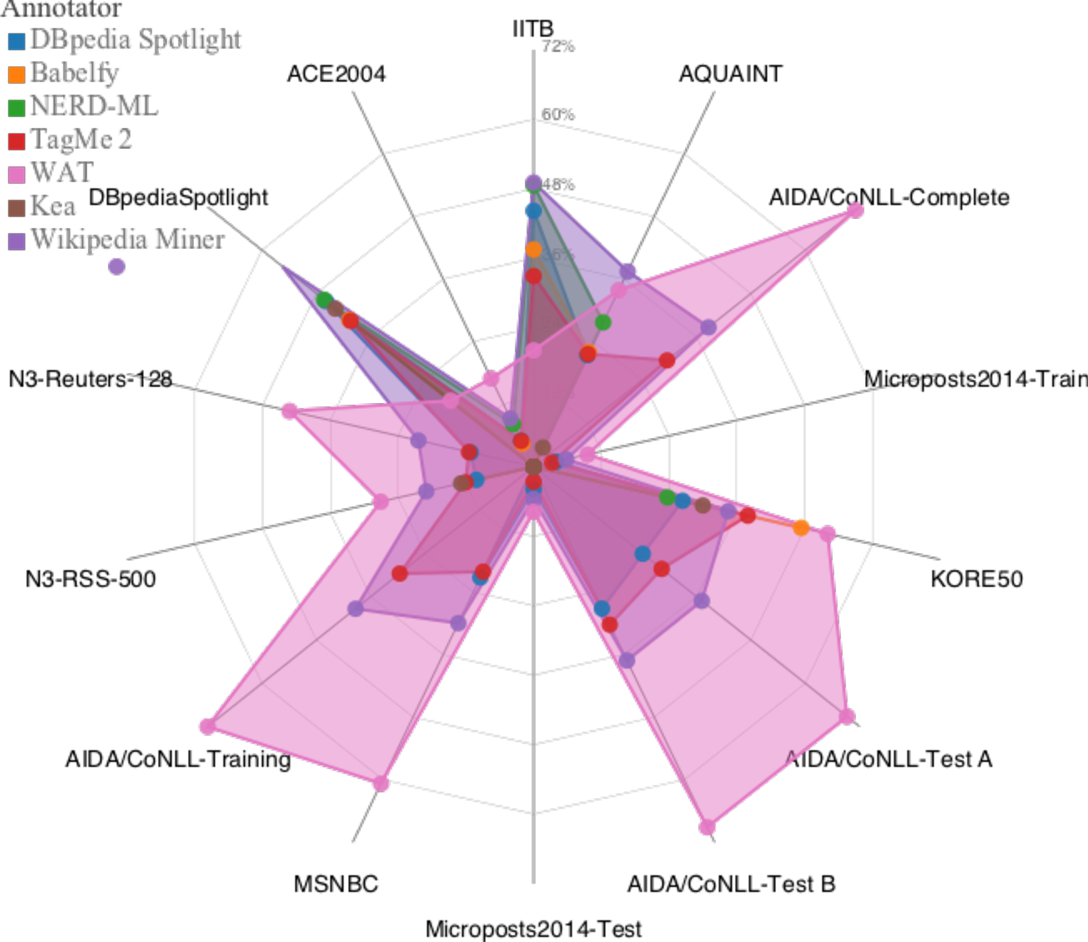
\includegraphics[width=0.5\textwidth]{part_02/benchmarking/WWW_GERBIL/spider}
%\caption{Example spider diagram of recent A2KB experiments with strong annotation matching derived from our online interface}
%\label{fig:spider}
%\end{figure}
%\todo[inline]{For each spider, say when it was pulled}


\section{Evaluation}
\label{cha332:sec:eval}
%GERBIL allows publishing, citing, reproducing and analysing entity annotation experiment data.

To ensure the practicability and convenience of the GERBIL framework, we investigated the effort needed to use GERBIL for the evaluation of novel annotators.
To achieve this goal, we surveyed the workload necessary to implement a novel annotator into GERBIL compared to the implementation into previous diverse frameworks.

Our survey comprised five developers with expert-level programming skills in Java. Each developer was asked to evaluate how much time he/she needed to write the code necessary to evaluate his/her framework on a new dataset.

%\todo[inline]{Add diagram showing time for own data/time on GERBIL}
\begin{figure}[tb!]
\centering
\includegraphics[width=\columnwidth]{part_02/benchmarking/WWW_GERBIL/user_study.eps}
\caption{Comparison of effort needed to implement an adapter for an annotation system with and without GERBIL.}
\label{ref:comparedTime}
\end{figure}
\todo[inline]{redo graphics}
%%\todo[inline]{Add diagram showing time for own data/time on GERBIL}
\begin{figure}
\centering
\includegraphics[width=\columnwidth]{part_02/benchmarking/WWW_GERBIL/user_study.eps}
\caption{Comparison of effort needed to implement an adapter for an annotation system with and without GERBIL.}
\label{ref:comparedTime}
\end{figure}


Overall, the developers reported that they needed between 1 and 4 hours to achieve this goal (4x 1-2h, 1x 3-4h), see Figure~\ref{ref:comparedTime}.
Importantly, all developers reported that they needed either the same or even less time to integrate their annotator into GERBIL.
This result in itself is of high practical significance as it means that by using GERBIL, developers can evaluate on (currently) \overalldatasets datasets using the same effort they needed for 1, which is a gain of more than 1100\%.
Moreover, all developers reported they felt comfortable---4 points on average on a 5-point Likert scale between very uncomfortable (1) and very comfortable (5)---implementing the annotator in GERBIL.
Further developers were invited to complete the survey, which is available at our project website.
%\url{ https://docs.google.com/spreadsheets/d/1v3EyAnHxA3zgfoL4CcqEM4_EbvpKiCWeg6qc3FOKf2o/edit#gid=414618098}
Even though small, this evaluation suggests that implementing against GERBIL does not lead to any overhead. On the contrary, GERBIL significantly improves the time-to-evaluation by offering means to benchmark and compare against other annotators respectively datasets within the same effort frame previously required to evaluate on a single dataset.

An interesting side-effect of having all these frameworks and datasets in a central framework is that we can now benchmark the different frameworks with respect to their runtimes within exactly the same experimental settings. These results are of practical concern for end users of annotation frameworks as they are most commonly interested in both the runtime and the quality of solutions. For example, we evaluated the runtimes of the different approaches in GERBIL for the A2KB experiment type on the MSNBC dataset. The results of this experiment are shown in Figure~\ref{fig:runtime}.


\begin{figure}[tb!]
\centering
\includegraphics[width=\columnwidth]{part_02/benchmarking/WWW_GERBIL/needed_times.eps}
\caption{Runtime per document of different approaches in GERBIL for the A2KB experiment type on the MSNBC dataset.}
\label{fig:runtime}
\end{figure}
\todo[inline]{redo graphics}
%\todo[inline]{@Micha runtime in s/document?}

%\subsection{Reproducibility of experiments}
%\label{sec:repro}
%\todo[inline]{ADD A2W, D2W benchmark tables here with URIs to proof GERBIL %works.}
%The main goal of GERBIL is to provide comprehensible experiments in the field of NER and NED.
%Especially, we are interested in reproducing the results of AGDISTIS~\cite{agdistis_iswc}, TagMe 2~\cite{TagMe2,Cornolti} and Babelfy~\cite{babelfy}.
\section{Current development of GERBIL}
\label{sec:currentNumbersForGERBIL}
\begin{itemize}
\item New numbers for datasets, annotators, experiment types, matchings
\item User numbers
\item describe changes from 1.0 to 1.2
\end{itemize}


\section{Conclusion and Future Work}
\label{cha332:sec:conclusion}
In this paper, we presented and evaluated GERBIL, a platform for the evaluation of annotation frameworks. With GERBIL, we aim to push annotation system developers to better quality and wider use of their frameworks.
Some of the main contributions of GERBIL include the provision of persistent URLs for reproducibility and archiving.
Furthermore, we implemented a generic adaptor for external datasets as well as a generic interface to integrate remote annotator systems.
The datasets available for evaluation in the previous benchmarking platforms for annotation was extended by \numberOfadditionalDatasets new datasets. Moreover, \numberOfadditionalAnnotators novel annotators were added to the platform. 
The evaluation of our framework by contributors suggests that adding an annotator to GERBIL demands 1 to 2 hours of work. Hence, while keeping the implementation effort previously required to evaluate on a single dataset, we allow developers to evaluate on (currently) \overalldatasets times more datasets.
The presented, web-based frontend allows for several use cases enabling laymen and expert users to perform informed  comparisons of semantic annotation tools.
The persistent URIs enhances the long term quotation in the field of information extraction.
GERBIL is not just a new framework wrapping existing technology. 
In comparison to earlier frameworks, it extends the state-of-the-art benchmarks by the capability of considering the influence of NIL attributes and the ability of dealing with data sets and annotators that link to different knowledge bases.
%GERBIL extends the state-of-the-art benchmarks by the capability of considering the influence of NIL attributes and the ability of dealing with data sets and annotators that link to different knowledge bases. 
%GERBIL is being updated continuously.
More information about GERBIL and its source code can be found at the project's website. 

%\todo[inline]{AnBo: Currently it sound like a wrapper framework for convenient programming. I would add the functional evolution comparing BAT as well. Suggestion:

%However, GERBIL is not just a new framework wrapping existing technology. 
%In comparison to earlier frameworks, it extends the state-of-the-art benchmarks by the capability of considering the influence of NIL attributes and the ability of dealing with data sets and annotators that link to different knowledge bases.
%AN: Done
%}

While developing GERBIL, we spotted several flaws in the formal model underlying previous benchmarking frameworks which we aim to tackle in the future. 
For example, the formal specification underlying current benchmarking frameworks for annotation does not allow using the scores assigned by the annotators for their results. To address this problem, we aim to develop/implement novel measures into GERBIL that make use of scores (e.g., Mean Reciprocal Rank). 
Moreover, partial results are not considered within the evaluation. For example, during the disambiguation task, named entities without Wikipedia URIs are not considered. This has a significant impact of the number of true and false positives and thus on the performance of some tools.
Furthermore, certain tasks seem to be too coarse. For example, we will consider splitting the Sa2KB and the A2KB tasks into two subtasks: The first subtask would measure how well tools perform at finding named entities inside the text (NER task) while the second would evaluate how well tools disambiguate those named entities which have been found correctly (similar to the D2KB task).
In future work, we also aim to provide a new theory for evaluating annotation systems and display this information in the GERBIL interface.
In the future, we also plan to provide information about the point in time since when an annotator is stable, i.e., the algorithm underlying the webservice has not changed.
GERBIL has sparked the idea for the succesful Horizon 2020 proposal HOBBIT and will influence the central architecture underlying the HOBBIT Big Linked Data Benchmarking Platform. 

%soi%\documentclass{llncs}

%\usepackage{graphicx}
%\usepackage{pifont}
%\usepackage{amsmath,amssymb}
%\usepackage[english]{babel}
%\usepackage[utf8]{inputenc}
%\usepackage[ruled,vlined]{algorithm2e}
%\usepackage{hyperref}
%\usepackage{float} 
%\usepackage{multirow} 
%\usepackage{booktabs}
%\usepackage[disable]{todonotes}
%\usepackage{todonotes}
%\usepackage{mdframed}
%\usepackage{wrapfig}
%\usepackage{booktabs}
%\usepackage{cha333:tabulary}
%\usepackage{caption}
%\usepackage{comment}
%\usepackage{tikz}
%\usepackage{xspace}
%\usepackage{times}
%\usepackage{subfigure}

%\newcommand{\haken}{{\ding{51}}}
%\newcommand*\rot{\rotatebox{87}}



%\begin{document}

\chapter{Evaluating Entity Annotators Using GERBIL}

%\author{
%Ricardo Usbeck \and 
%Michael Röder \and
%Axel-Cyrille Ngonga Ngomo
%}

%\institute{
%University of Leipzig, Germany\\\email{\{usbeck,roeder,ngonga\}@informatik.uni-leipzig.de}
%}

%\maketitle

%\begin{abstract}
The need to bridge between the unstructured data on the Document Web and the structured data on the Web of Data has led to the development of a considerable number of annotation tools. However, these tools are hard to compare due to the diversity of data sets and measures used for evaluation. 
We will demonstrate GERBIL, an evaluation framework for semantic entity annotation that provides developers, end users and researchers with easy-to-use interfaces for the agile, fine-grained and uniform evaluation of annotation tools on 11 different data sets within 6 different experimental settings on 6 different measures. 
%We present the different types of experiments as well as the human-readable and machine-readable output formats supported by GERBIL. In addition, we show how the permanent experiment URIs provided by GERBIL ensure the reproducibility and archiving of evaluation results. Finally, we show how GERBIL can provide developers with diagnostics that allow to spot current strengths and weaknesses of their annotators. 
%\end{abstract}


\section{Introduction}
%The implementation of the original vision behind the Semantic Web demands the development of approaches and frameworks for the seamless extraction of structured data from text. 
The need for extracting structured data from text has led to the development of a large number of tools dedicated to the extraction of structured data from unstructured data (see~\cite{GERBIL} for an overview).
% \cite{TagMe2,AIDA,spotlight,milne2008learning,babelfy,piccinno2014tagme,rizzo2014,Steinmetz2013,AGDISTIS_ISWC}. Still, the provision of comparable results for these tools remains a tedious problem. 
%The issue of  comparability of results is not to be regarded as being intrinsic to the annotation task.% Indeed, it is now well established that scientists spend between 60 and 80\% of their time preparing data for experiments \cite{GIL2014,jermyn1999preparing,peng2011reproducible}.
%Data preparation being such a tedious problem in the annotation domain is mostly due to the different formats of the gold standards as well as the different data representations across reference data sets.
%
%These restrictions have led to authors evaluating their approaches on data sets (1) that are available to them and (2) for which writing a parser as well as of an evaluation tool can be carried out with reasonable effort.
%In addition, a large number of quality measures have been developed and used actively across the annotation research community to evaluate the same task, leading to the results across publications on the same topics not being easily comparable. For example, while some authors publish macro-F-measures and simply call them F-measures, others publish micro-F-measures for the same purpose, leading to significant discrepancies across the scores. The same holds for the evaluation of how well entities match. Indeed, partial matches and complete matches have been used in previous evaluations of annotation tools \cite{Cornolti,fox}. This heterogeneous landscape of tools, data sets and measures leads to a poor repeatability of experiments, which makes the evaluation of the real performance of novel approaches against the state of the art rather difficult.
%Recently, various benchmarking framework for entity annotation systems occurred focusing on different aspects.
%The BAT-framework~\cite{Cornolti} is designed to facilitate the benchmarking of named entity recognition (NER), named entity disambiguation (NED) and concept tagging approaches.
%BAT compares seven existing entity annotation approaches using Wikipedia as reference, and offers six different task types, five different matchings and six evaluation measures providing five data sets.
%Rizzo et al.~\cite{rizzo2014} present a state-of-the-art study of NER and NEL systems for annotating newswire and micropost.
In this demo, we present GERBIL, a framework for the evaluation of entity annotation frameworks. GERBIL provides a GUI that allows (1) configuring and running experiments, (2) assigning persistent URLs to experiments (better reproducibility and archiving), (3) exporting the results of the experiments in human- and machine-readable formats as well as (4) displaying the results w.r.t. the data sets and the features of the data sets on which the experiments were performed. %By these means, GERBIL goes beyond the state of the art by extending the BAT-framework~\cite{Cornolti} as well as~\cite{rizzo2014} in several dimensions to enhance reproducibility, diagnostics and publishability of the results  of entity annotation systems. 

%In this paper, we present GERBIL -- a general entity annotator benchmark --, a community-driven effort to enable the continuous evaluation of annotation tools. 
GERBIL is an open-source and extensible framework that allows evaluating tools against (currently) \overallGERBILannotators different annotators on \overalldatasets different data sets within 6 different experiment types. 
%By integrating such a large number of data sets, experiment types and frameworks, GERBIL allows users to evaluate their tools against other semantic entity annotation systems (short: entity annotation systems) by using exactly the same setting, leading to fair comparisons based on exactly the same measures. 
%While the evaluation core of GERBIL is based on the BAT-framework \cite{Cornolti}, our approach goes beyond the state of the art in several respects:
%\begin{itemize}
%\item GERBIL provides \emph{persistent URLs} for experimental settings. Hence, by using GERBIL for experiments, tool developers can ensure that the settings for their experiments (measures, data sets, versions of the reference frameworks, etc.) can be reconstructed in a  unique manner in future works. 
%\item Through experiment URLs, GERBIL also addresses the problem of \emph{archiving} experimental results and allows end users to gather all pieces of information required to choose annotation frameworks for practical applications.
%\item GERBIL aims to be a \emph{central repository for annotation results} without being a central point of failure: While we make experiment URLs available, we also provide users directly with their results to ensure that they use them locally without having to rely on GERBIL.
%\item The results of GERBIL are published in a \emph{machine-readable format}. In particular, our use of DataID~\cite{dataID} to denote tools and data sets ensures that results can be easily combined and queried (for example to study the evolution of the performance of frameworks) while the exact configuration of the experiments remains uniquely reconstructable. By these means, we also tackle the problem of \emph{reproducibility}. 
%\item Through the provision of results on different data sets of different types and the provision of results on a simple user interface, GERBIL also provides means to quickly gain an overview of the current performance of annotation tools, thus providing (1) developers with insights pertaining to the type of data on which their accuracy needs improvement and (2) end users with insights allowing them to choose the right tool for the tasks at hand.
%\item With GERBIL we introduce the notion of knowledge base-agnostic benchmarking of entity annotation systems through generalized experiment types. By these means, we allow benchmarking tools against reference data sets from any domain grounded in any reference knowledge base. 
%\end{itemize}
To ensure that our framework is useful to both end users and tool developers, its architecture and interface were designed to allow (1) the easy integration of annotators through REST services, (2) the easy integration of data sets via DataHub\footnote{\url{http://datahub.io}}, file uploads or direct source code integration, (3) the addition of new performance measures, (4) the provision of diagnostics for tool developers and (5) the portability of results. 
%\begin{itemize}
%\item \textbf{Easy integration of annotators}: We provide a wrapping interface that allows annotators to be evaluated via their REST interface. In particular, we integrated \numberOfadditionalAnnotators additional annotators not evaluated against each other in previous works (e.g., \cite{Cornolti}).  
%\item \textbf{Easy integration of data sets}: We also provide means to gather data sets for evaluation directly from data services such as DataHub.\footnote{\url{http://datahub.io}} In particular, we added \numberOfadditionaldata sets new data sets to GERBIL.
%\item \textbf{Easy addition of new measures}: The evaluation measures used by GERBIL are implemented as interfaces. Thus, the framework can be easily extended with novel measures devised by the annotation community.
%\item \textbf{Extensibility}: GERBIL is provided as an open-source platform\footnote{Available at \url{http://gerbil.aksw.org}.} that can be extended by members of the community both to new tasks and different purposes.
%\item \textbf{Diagnostics}: The interface of the tool was designed to provide developers with means to easily detect aspects in which their tool(s) need(s) to be improved. 
%\item \textbf{Portability of results}: We generate human- and machine-readable results to ensure maximum usefulness and portability of the results generated by our framework. 
%\end{itemize}
%\todo[inline]{summarize rest}
More information on GERBIL as well as a link to the online demo can be found at the project webpage at \url{http://gerbil.aksw.org}.
%and at the code repository page \url{https://github.com/AKSW/gerbil}
%The online version of this demo can be accessed at \url{http://gerbil.aksw.org/gerbil}. 
%This paper is a demo paper to the WWW 2015 paper \cite{GERBIL}.

%\todo[inline]{What will be shown in the demo?}
\section{GERBIL in a nutshell}
\label{cha333:sec:architecture}
\begin{figure}[tb]
\centering
%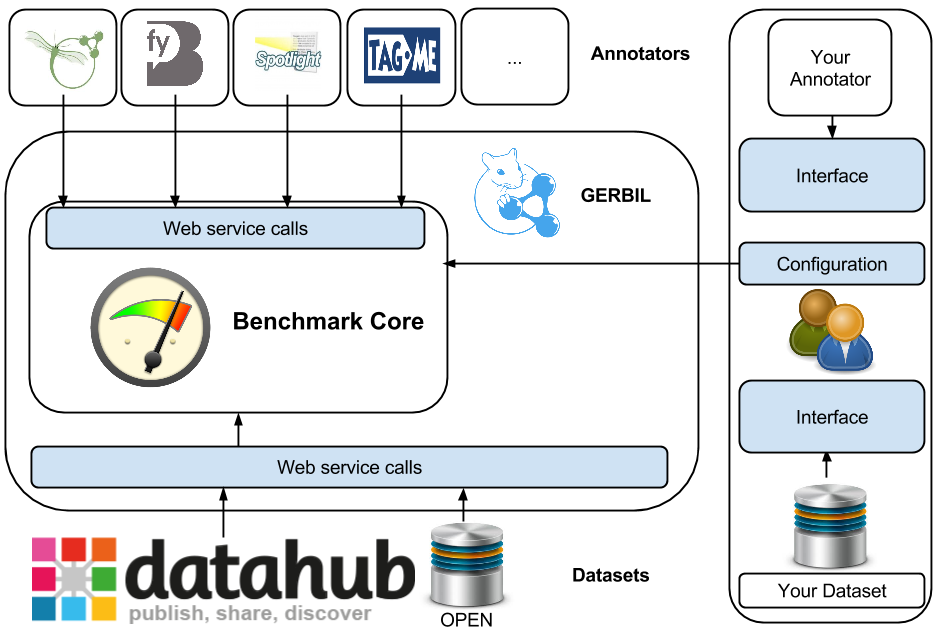
\includegraphics[width=\linewidth]{GERBIL_new_architectur}
\includegraphics[width=0.7\linewidth]{part_02/benchmarking/ESWC_GERBIL_demo/gerbiloverview.eps}
%\vspace{-5mm}
\caption{Overview of GERBIL's abstract architecture. Interfaces to users and providers of data sets and annotators are marked in blue.
}
\label{cha333:fig:architecture}
%\vspace{-2mm}
\end{figure}

An overview of GERBIL's architecture is given in Figure~\ref{cha333:fig:architecture}. 
Based on this architecture, we will explain the features that we will present in the demonstration of the GERBIL framework.
%All features will be presented through the online demo at \url{http://gerbil.aksw.org/gerbil}.

\begin{figure}[htb]
\centering
\includegraphics[width=\textwidth]{part_02/benchmarking/ESWC_GERBIL_demo/results.pdf}
\caption{Example spider diagram of recent A2KB experiments with weak annotation matching.}
\label{cha333:fig:spiderfmeasure}
\end{figure}

\begin{figure}[htb]
\centering
\includegraphics[width=\textwidth]{part_02/benchmarking/ESWC_GERBIL_demo/correlations.pdf}
\caption{Spider diagram of correlations between annotation results and data set features.}
\label{cha333:fig:spiderfeature}
\end{figure}


\begin{wrapfigure}{l}{6cm}
\centering
\includegraphics[width=0.95\linewidth]{part_02/benchmarking/ESWC_GERBIL_demo/screenshot}
\caption{Experiment configuration screen.}
\label{cha333:fig:screenshot}
\end{wrapfigure}

\textbf{Feature 1: Experiment types.}
An experiment type defines the way used to solve a certain problem when extracting information.
GERBIL extends the six experiments types provided by the BAT framework~\cite{cornolti} (including entity recognition and disambiguation). 
%and extends them by the idea to not only link to Wikipedia but to any knowledge base $K$, see~\cite{GERBIL}.
%The six experiment types implemented in GERBIL are (1) \emph{D2KB}, i.e., disambiguating a set of \emph{given} entity mentions to entities from a given knowledge base or to NIL, (2) \emph{A2KB}, i.e., the classical NER/D task also available as (3) \emph{Sa2KB}, which is the scored annotation task, as well as (4) \emph{C2KB}, i.e., the concept tagging task which aims to detect entities in a given document, also available in a scored variant (\emph{Sc2KB}) and a ranked (\emph{Rc2KB}) version.
With this extension, our framework can deal with gold standard data sets and annotators that link to any knowledge base, e.g., DBpedia, BabelNet~\cite{NavigliPonzetto:12aij} etc., as long as the necessary identifiers are URIs. During the demo, we will show how users can select the type of experiments in the interface (see Figure~\ref{cha333:fig:screenshot}) and explain the different types of experiments.\newline


%\begin{minipage}{0.48\textwidth}
%\end{minipage}
%\hfill
%\begin{minipage}{0.48\textwidth}
%\begin{cha333:table}[htb]
%\centering
%\captionof{cha333:table}{Implemented annotator systems. }
%\label{cha333:tab:annotator}
%\begin{cha333:tabulary}{\columnwidth}{LLC}
%\toprule
%\multicolumn{2}{c}{Annotator}& Experiment\\ 
%\midrule
%\multirow{2}{*}{\cite{milne2008learning}}&Wikipedia                     &\multirow{2}{*}{SA2KB}\\
%&Miner                     &\\
%\cite{rat:rot}&Illionois Wikifier       & SA2KB\\
%\cite{spotlight}&Spotlight            & SA2KB\\
%\cite{TagMe2}&TagMe 2                 & SA2KB\\
%\cite{AIDA}&AIDA                      & SA2KB\\
%\cite{Steinmetz2013}&KEA              & SA2KB\\
%\cite{piccinno2014tagme}&WAT          & SA2KB\\
%\cite{AGDISTIS_ISWC}&AGDISTIS         & D2KB\\
%\cite{babelfy}&Babelfy                & SA2KB\\
%\cite{rizzo2014}&NERD-ML              & SA2KB\\
%\cite{ceccarelli2013dexter}&Dexter   & SA2KB\\
%&NIF-based                     &\multirow{2}{*}{any}\\
%&Annotator                     &\\
%\bottomrule
%\end{cha333:tabulary}
%\end{cha333:table}
%\end{minipage}

%\todo[inline]{AN: Add figure showing the selection of experiment types and matchings. Add reference here and  below (matching section).}

\textbf{Feature 2: Matchings.}
GERBIL offers three types of matching between a gold standard and the results of annotation systems: a \emph{strong entity matching} for URLs, as well as a  \emph{strong} and a \emph{weak annotation matching} for entities.
%(3) \emph{Weak annotation matching $M_w$} has been introduced to relax certain cases. For example,  a gold standard contains a named entity "President Barack Obama" while the result of an annotator only marks "Barack Obama" as named entity. Using an exact matching leads to weighting this result as wrong while a human might rate it as correct. Thus, a correct annotation has to be linked to the same entity and must overlap the annotation of the gold standard.
%(3) \emph{Weak annotation matching $M_w$} relaxes the condition of $M_a$ regarding the position of the entity to allow overlap with the annotation of the gold standard.
The selection and an explanation of the types of matching for given experiments will be part of the demo (see Figure~\ref{cha333:fig:screenshot}). %\todo[inline]{AN: Add ref to figure as requested above.}

\textbf{Feature 3: Metrics.}
Currently, GERBIL offers six measures subdivided into two groups: the micro- and the macro-group of precision, recall and f-measure. As shown in Figure~\ref{cha333:fig:spiderfmeasure}, these results are displayed using interactive spider diagrams that allow the user to easily (1) get an overview of the performance of single tools, (2) compare tools with each other and (3) gather information on the performance on tools on particular data sets. We will show how to interact with our spider diagrams during the demo.

\textbf{Feature 4: Diagnostics.}
An important novel feature of our interface is that it displays the correlation between the features of data sets and the performance of tools (see Figure~\ref{cha333:fig:spiderfeature}). By these means, we ensure that developers can easily gain an overview of the performance of tools w.r.t. a set of features and thus detect possible areas of improvement for future work. 
%End users can make use of these results to select the right tool for their current requirements. Currently, we display correlations with the following data set features: (1) number of documents and (2) number of entities in the data set, (3) entities per document, (4) entities per token, (5) average length of a document as well as (6) the number  of entities of the different types (persons, locations, organizations, etc.). The interface provides these scores by using spider diagrams akin to those used to display the evaluation metrics. We will also show the diagnostics diagrams and explain how to interact with them during the demo. 

\textbf{Feature 5: Annotators.}
The main goal of GERBIL is to simplify the comparison of novel and existing entity annotation systems in a comprehensive and reproducible way.
Therefore, GERBIL offers several  ways to implement novel entity annotation frameworks.
We will show how to integrate annotators into GERBIL by using a Java adapter as well as a \emph{NIF-based Service}~\cite{NIF}.% for communication over web-service in two ways
%: i) if the server-side implementation of annotators understands NIF-documents as input and output format, GERBIL and the framework can simply exchange NIF-documents or ii) if developers do not want to publish their APIs or write source code, GERBIL offers the possibility for NIF-based webservices to be tested online by providing their URI and name only.\footnote{\url{http://gerbil.aksw.org/gerbil/config}} GERBIL does not store these connections in terms of API keys or URLs but still offers the opportunity of persistent experiment results.
Currently, GERBIL offers \overallGERBILannotators entity annotation systems with a variety of features, capabilities and experiments out-of-the-box, including Illinois Wikifier, DBpedia Spotlight, TagMe, AIDA, KEA, WAT, AGDISTIS, Babelfy, NERD-ML and Dexter~\cite{GERBIL}.   
%Table~\ref{cha333:tab:annotator} presents the provided systems and their supported experiment types.
%While AGDISTIS has been in the source code of the BAT-Framework provided by a third-party after publication of Cornolti et al.'s initial work~\cite{Cornolti} in 2014, GERBIL's community effort led to the implementation of overall \numberOfadditionalAnnotators new annotators as well as the before mentioned generic NIF-based annotator.
%The AIDA annotator as well as the "Illinois Wikifier" will not be available in GERBIL since we restrict ourselves to webservices.
%However, these algorithms can be integrated at any time as soon as their webservices are available.
%Upon request, we will show how to integrate annotators into GERBIL by any of these two ways. Especially, we will explain the format of the output that must be generated by a system for GERBIL to be able to interprete it.

\textbf{Feature 6: Data sets.}
Table~\ref{cha333:tab:corpus_stats} shows the \overalldatasets data sets available via GERBIL. 
Thank to the large number of formats, topics and features of the datasets, GERBIL allows carrying out diverse experiments. During the demo, we will show how to add more data sets to GERBIL.

\begin{table*}
    \caption{Features of the data sets and their documents.}
    \begin{tabular}{lp{0.25cm}rp{0.25cm}rp{0.25cm}rp{0.25cm}rp{0.25cm}r}
     \toprule
     Corpus && Topic &&Format &&Experiment && \multicolumn{1}{c}{Size} && \multicolumn{1}{c}{Avg. Entity/Doc.} \\
    \midrule
ACE2004          && news        && MSNBC    && Sa2KB    &&   57 &&   4.44\\
AIDA/CoNLL       && news        && CoNLL    && Sa2KB    && 1393 &&  19.97\\
Aquaint          && news        &&  -       && Sa2KB    &&   50 &&  14.54\\
IITB             && mixed       && XML      && Sa2KB    &&  103 && 109.22\\
KORE 50          && mixed       && NIF/RDF  && Sa2KB    &&   50 &&   2.86\\
Meij             && tweets      && TREC     && Rc2KB    &&  502 &&   1.62\\
Microposts2014   && tweets      &&  -       && Sa2KB    && 3505 &&   0.65\\
MSNBC            && news        && MSNBC    && Sa2KB    &&   20 &&  32.50\\
N$^3$ Reuters-128&& news        && NIF/RDF  && Sa2KB    &&  128 &&   4.85\\
N$^3$ RSS-500    && RSS-feeds   && NIF/RDF  && Sa2KB    &&  500 &&   0.99\\
Spotlight Corpus && news        && NIF/RDF  && Sa2KB    &&   58 &&   5.69\\
%Wiki             && encyclopedic    &&   ? &&   ?\\
	\bottomrule
	\end{tabular}
	\centering
	\label{cha333:tab:corpus_stats}
\end{table*}

%Moreover, we capitalize upon the uptake of publicly available, NIF based corpora over the last years~\cite{yovisto,N3}\footnote{\url{http://datahub.io/data set?license_id=cc-by&q=NIF}}.
%To this end, GERBIL implements a Java-based NIF~\cite{NIF} reader and writer module which enables loading arbitrary NIF document collections, as well as the communication to NIF-based webservices.
%The extensibility of the data sets in GERBIL is furthermore ensured by allowing users to upload or use already available NIF data sets from DataHub. 
%GERBIL will regularly check whether new corpora are available and publish them for benchmarking after a manual quality assurance cycle which ensures their usability for the implemented configuration options.
%Additionally, users can upload their NIF-corpora directly to GERBIL avoiding their publication in publicly available sources.
%This option allows for rapid testing of entity annotation systems with closed source or licenced data sets.

\textbf{Feature 7: Output.}
\label{cha333:sec:output}
GERBIL's main aim is to provide comprehensive, reproducible and publishable experiment results.
Hence, GERBIL's experimental output is represented as a table containing the results, as well as embedded JSON-LD\footnote{\url{http://www.w3.org/TR/json-ld/}} RDF data. During the demo, we will show the output generated by GERBIL for the different experiments implemented and show how the RDF results can be used for the sake of archiving  results. Moreover, we will show how to retrieve experimental results using the permanent URI generated by GERBIL. %We will also show how the results can be queried using SPARQL.

% using the RDF DataCube vocabulary~\cite{datacube}.
%We ensure a detailed description of each component of an experiment as well as machine-readable, interlinkable results following the 5-star Linked Data principles using Linked SDMX~\cite{LinkedSDMX} and DataID~\cite{dataID}.
%Moreover, we provide a persistent and time-stamped URL for each experiment, see Table~\ref{cha333:tab:persistentURL}.

%\begin{cha333:table}
%    \begin{cha333:tabular}{lcr}
%    \toprule
%    Annotator & data set & F1-micro \\
%    \midrule
%    DBpedia Spotlight & IITB & 0.444 \\
%    Babelfy & IITB & 0.377 \\
%    NERD-ML & IITB & 0.488 \\
%    WAT & IITB & 0.202 \\
%    DBpedia Spotlight & KORE50 & 0.265 \\
%    Babelfy & KORE50 & 0.476 \\
%    NERD-ML & KORE50 & 0.238 \\
%    WAT & KORE50 & 0.523 \\
%	\bottomrule
%	\end{cha333:tabular}
%	\centering
%    \caption{Results of an example experiment. It is accessible at \url{http://gerbil.aksw.org/gerbil/experiment?id=201411100001}}
%	\label{cha333:tab:persistentURL}
%\end{cha333:table}

%\emph{RDF DataCube} is a vocabulary standard and can be used to represent fine-grained multidimensional, statistical data which is compatible with the  Linked SDMX~\cite{LinkedSDMX} standard. 
%Every GERBIL experiment is modelled as \texttt{qb:data set} containing the individual runs of the annotators on specific corpora as \texttt{qb:Observations}. 
%Each observation features the \texttt{qb:Dimensions} experiment type, matching type, annotator, corpus and time. 
%The six evaluation measures offered by GERBIL as well as the error count are expressed as \texttt{qb:Measures}. 
%To include further metadata, annotator and corpus dimension properties link \emph{DataID}~\cite{dataID} descriptions of the individual components. 

%GERBIL uses the recently proposed DataID~\cite{dataID} ontology that combines VoID~\cite{void} and DCAT~\cite{dcat} metadata with Prov-O~\cite{prov-o} provenance information and ODRL~\cite{odrl} licenses to describe data sets.
%Besides metadata properties like titles, descriptions and authors, the source files of the open data sets themselves are linked as \texttt{dcat:Distributions}, allowing direct access to the evaluation corpora. 
%Furthermore, ODRL license specifications in RDF are linked via \texttt{dc:license}, potentially facilitating automatically adjusted processing of licensed data by NLP tools. 
%Licenses are further specified via \texttt{dc:rights}, including citations of the relevant publications. 

%To describe annotators in a similar fashion, we extended DataID for services. 
%The class \texttt{Service}, to be described with the same basic properties as data set, was introduced. 
%To link an instance of a \texttt{Service} to its distribution the \texttt{datid:distribution} property was introduced as super property of \texttt{dcat:distribution}, i.e., the specific URI the service can be queried at.
%Furthermore, Services can have a number of \texttt{datid:Parameters} and \texttt{datid:Configurations}.
%data sets can be linked via \texttt{datid:input} or \texttt{datid:output}. 

%Offering such detailed and structured experimental results opens new research avenues in terms of tool and data set diagnostics to increase decision makers' ability to choose the right settings for the right use case.

\section{Evaluation}
\label{cha333:sec:eval}
To ensure that GERBIL can be used in practical settings, we investigated the effort needed to use GERBIL for the evaluation of novel annotators.
To achieve this goal, we surveyed the workload necessary to implement a novel annotator into GERBIL compared to the implementation into previous diverse frameworks. 
Our survey comprised five developers with expert-level programming skills in Java. Each developer was asked to evaluate how much time he/she needed to write the code necessary to evaluate his/her framework on a new data set.
Further details pertaining to this evaluation are reported in the research paper to this demo \cite{GERBIL}.


Overall, the developers reported that they needed between 1 and 4 hours to achieve this goal (4x 1-2h, 1x 3-4h), see Figure~\ref{cha333:fig:comparedTime}.
Importantly, all developers reported that they needed either the same or even less time to integrate their annotator into GERBIL.
This result in itself is of high practical significance as it means that by using GERBIL, developers can evaluate on (currently) \overalldatasets data sets using the same effort they needed for 1, which is a gain of more than 1100\%.
Moreover, all developers reported they felt comfortable---4 points on average on a 5-point Likert scale between very uncomfortable (1) and very comfortable (5)---implementing the annotator in GERBIL.
%Further developers were invited to complete the survey, which is available at our project website.
Even though small, this evaluation suggests that implementing against GERBIL does not lead to any overhead.
Furthermore, the interviewed developers represent a majority of the active research and development community in the are of entity annotation systems.
%On the contrary, GERBIL significantly improves the time-to-evaluation by offering means to benchmark and compare against other annotators respectively data sets within the same effort frame previously required to evaluate on a single data set.

An interesting side-effect of having all these frameworks and data sets in a central framework is that we can now benchmark the different frameworks with respect to their runtimes within exactly the same experimental settings. 
%These results are of practical concern for end users of annotation frameworks as they are most commonly interested in both the runtime and the quality of solutions. 
For example, we evaluated the runtimes of the different approach\-es in GERBIL for the A2KB experiment type on the MSNBC data set, see Figure~\ref{cha333:fig:runtime}.


\begin{figure}[ht]
\centering
\includegraphics[width=0.48\textwidth]{part_02/benchmarking/ESWC_GERBIL_demo/user_study.eps}
\caption{Comparison of effort needed to implement an adapter for an annotation system.}
\label{cha333:fig:comparedTime}
%\captionof{cha333:figure}{Example spider diagram of recent A2KB experiments with weak annotation matching derived from our online interface.}
\end{figure}

\begin{figure}[ht]
\centering
\includegraphics[width=0.48\textwidth]{part_02/benchmarking/ESWC_GERBIL_demo/needed_times.eps}
%\captionof{cha333:figure}{Spider diagram of results of figure \ref{cha333:fig:spiderfmeasure} and their correlation to data set features.}
\caption{Runtime per document for the A2KB experiment type on the MSNBC data set.}
\label{cha333:fig:runtime}
\end{figure}

\begin{comment}
\section{User Interface}
\label{cha333:sec:usecase}
Compliant with the main goal of GERBIL the reproduction of a certain experiment is central to facilitating research efforts. 
Therefore, our web-based platform offers the opportunity to configure an experiment using the parameters defined in Section~\ref{cha333:sec:architecture}.
The results will be displayed as described above and the experiment itself has a time-stamped URL which is citable and will be stable over time smoothing the way to a new citation quality.
Next to individual configurable experiments, GERBIL offers an overview of recent experiment results and correlations to data set features belonging to the same experiment and matching type in the form of a table as well as sophisticated visualizations\footnote{\url{http://gerbil.aksw.org/gerbil/overview}}, see Figure~\ref{cha333:fig:spiderfmeasure} and Figure~\ref{cha333:fig:spiderfeature}.
This allows for a quick comparison of tools and data sets on recently run experiments without additional computational effort.


\todo[inline]{This is a repetition of section 2.}
\textbf{Adding data sets and annotators.}
GERBIL is designed to be extensible, especially w.r.t. novel data sets and entity annotation systems.
Therefore, we differentiate three ways of integrating such data sets.
(1) A user can upload a NIF-based corpus of documents via our web-interface.
(2) GERBIL downloads data sets from \url{datahub.io} which we will then pull via HTTP requests which will be available after manual revision.
(3) Users can also implement a new data set wrapper source code-wise. 
If users than decide to integrate their wrappers intp GERBILs public repository the community will be further-on able to use it for public evaluations.

Additionally, users can submit new webservice-based entity annotation systems in two different ways:
(1) By providing us with the necessary information to call their NIF-based webservice.
Thereby, they need to enter the webservice's URI and a name for the algorithm.
This methods enables fast prototyping of webservices without the need to implement a BAT-framework annotator wrapper.
To lower barriers, we provide a NIF converter in Java.
(2) Additionally, a user can use our source code project, implement a new annotator and push his source code back to us. 
After a feasibility check, we will then bring the enhanced version of GERBIL online and announce it on the website.
Thus, a tremendous gain with respect to possible comparison opportunities in terms of annotators and data sets is inflicted.

GERBIL also provides an opportunity for closed source data\-set evaluation, e.g., business-relevant data or just experimental data not yet ready to be published.
Users can upload their NIF-based data set via GERBILs web interface.
Apart from the experiment results calculated with it, GERBIL will keep \emph{no} other data of such a data set.
\end{comment}

\section{Conclusion and Future Work}
\label{cha333:sec:conclusion}
In this paper, we presented a demo for GERBIL, a platform for the evaluation of annotation frameworks. We presented the different features that make the GERBIL interface easy to use and informative both for end users and developers. 
With GERBIL, we aim to push annotation system developers to better quality and wider use of their frameworks as well as include the provision of persistent URLs for reproducibility and archiving.
%Furthermore, we implemented a generic adaptor for external data sets as well as a generic interface to integrate remote annotator systems.
%The data sets available for evaluation in the previous benchmarking platforms for annotation was extended by \numberOfadditionaldata sets new data sets. Moreover, \numberOfadditionalAnnotators novel annotators were added to the platform. 
%The evaluation of our framework by contributors suggests that adding an annotator to GERBIL demands 1 to 2 hours of work.
%Hence, while keeping the implementation effort previously required to evaluate on a single data set, we allow developers to evaluate on (currently) \overalldata sets times more data sets.
%The presented, web-based frontend allows for several use cases enabling laymen and expert users to perform informed comparisons of semantic annotation tools and spot flaws w.r.t. the used data set features.
%The persistent URIs enhances the long term quotation in the field of information extraction.
%GERBIL is not just a new framework wrapping existing technology. 
%In comparison to earlier frameworks, it 
GERBIL extends the state-of-the-art benchmarks by the capability of considering the influence of NIL attributes and the ability of dealing with data sets and annotators that link to different knowledge bases. In future work, we aim to provide a new theory for evaluating annotation systems and display this information in the GERBIL interface.
%More information about GERBIL and its source code can be found at the project's website. 

%While developing GERBIL, we spotted several flaws in the formal model underlying previous benchmarking frameworks which we aim to tackle in the future. 
%For example, the formal specification underlying current benchmarking frameworks for annotation does not allow using the scores assigned by the annotators for their results. To address this problem, we aim to develop/implement novel measures into GERBIL that make use of scores (e.g., Mean Reciprocal Rank). 
%Moreover, partial results are not considered within the evaluation. For example, during the disambiguation task, named entities without Wikipedia URIs are not considered. This has a significant impact of the number of true and false positives and thus on the performance of some tools.
%Furthermore, certain tasks seem to be too coarse. For example, we will consider splitting the Sa2KB and the A2KB tasks into two subtasks: The first subtask would measure how well tools perform at finding named entities inside the text (NER task) while the second would evaluate how well tools disambiguate those named entities which have been found correctly (similar to the D2KB task).
%Moreover, we plan to provide information about the point in time since when an annotator is stable, i.e., the algorithm underlying the webservice has not changed so as to provide end users with metadata on when to use which annotator.


%\bibliographystyle{abbrv}
%\bibliography{myrefs}


%\end{document}
%

\chapter{Developing a Sustainable Platform for Entity Annotation Benchmarks}

%\author{
%Michael Röder \and
%Ricardo Usbeck \and 
%Axel-Cyrille Ngonga Ngomo
%}

%\institute{
%University of Leipzig, Germany\\\email{\{roeder,usbeck,ngonga\}@informatik.uni-leipzig.de}
%}

%\maketitle
%\todo[inline]{Focus on lessons learnt, mention how people can use your software. Accepted development papers will be published in the CEUR-WS workshop proceedings series.}

%\begin{abstract}
The existing entity annotation systems that drive the extraction of RDF from unstructured data are hard to compare as their evaluation relies on different data sets and measures. 
%growing amount of unstructured data on the Document Web and the rising number of tools for structured data from the Web of Data created the need for a growing
%number of entity annotation systems is hard to compare, making it difficult for developers to decide their published experiments are nearly unrepeatable and the diversity of data sets is tremendous.
We developed GERBIL, an evaluation framework for semantic entity annotation that provides developers, end users and researchers with easy-to-use interfaces for the agile, fine-grained and uniform evaluation of 9 annotation tools on 11 different data sets within 6 different experimental settings on 6 different measures. 
In this paper, we present the developed interfaces, data flows and data structures. Moreover, we show how GERBIL supports a better reproducibility and archiving of experimental results.
%Finally, we will explain how to use GERBIL from various perspectives and discuss why this community effort will support semantic annotation research in the long term.
%\end{abstract}


\section{Introduction}
The need for extracting structured data from text has led to the development of a large number of tools dedicated to the extraction of structured data from unstructured data (see~\cite{GERBIL} for an overview).
%The issue of  comparability of results is not to be regarded as being intrinsic to the annotation task.
While these tools do provide evaluation results, these results are rarely fully comparable as they commonly rely on different data sets or different measures. This is partly due to data preparation being a tedious problem in the annotation domain due to the different formats of the gold standards as well as the different data representations across reference data sets.
%These restrictions have led to authors evaluating their approaches on data sets (1) that are available to them and (2) for which writing a parser as well as of (3) an evaluation tool can be carried out with reasonable effort.
%Furthermore, diverse (4) quality measures have been developed and used actively across the annotation research community to evaluate the same task, leading to different results across publications which are not easily comparable. 
Recently, benchmarking frameworks such as the BAT-framework~\cite{cornolti} or NERD-ML~\cite{rizzo2014} for entity annotation systems have began addressing the problem on reproducible experiments for entity annotation.
With GERBIL\footnote{More information and a demo can be found at \url{http://gerbil.aksw.org}} 
 we aim to unify experiment setups, ease implementation and testing effort as well as contribute to an open, repeatable, publishable and archivable open science area to foster an active community of entity annotation tool developers. 

GERBIL goes beyond the state of the art by extending the BAT-framework~\cite{cornolti} as well as Nerd-ML~\cite{rizzo2014} in several dimensions. In particular we provide fine-grained diagnostics for annotation tools, enhanced reproducibility through archiving experiments and assigning URIs to them, easily publishable results by providing results both as RDF (for machines) and tables (for humans).
Overall, we provide the following features:

\textbf{Feature 1: Extensible experiment types.}
An experiment type defines the way used to solve a certain problem when extracting information.
GERBIL extends the six experiment types provided by the BAT framework~\cite{cornolti} (including entity recognition and disambiguation) towards more general, URI based experiments.
%Additionally, we are working on the implementation of an entity typing experiment as it is defined in the Open Knowledge Extraction Challenge 2015\footnote{\url{http://2015.eswc-conferences.org/important-dates/call-OKEC}}.
% as well as it implements 3 experiment types for the Open Knowledge Extraction Challenge 2015\footnote{\url{http://2015.eswc-conferences.org/important-dates/call-OKEC}}.
%\todo[inline]{Micha: Ich finde das nicht so gut, dass wir immer Dinge ins Paper schreiben, die wir noch gar nicht gemacht haben. Wir können gern reinschreiben, dass wir das "Entity Typing" als weiteren Experimenttyp einbringen. Aber mehr haben wir im Moment ja noch gar nicht.}
With this extension, our framework can deal with gold standard data sets and annotators that link to any knowledge base as long as the necessary identifiers are URIs.

\textbf{Feature 2: Matchings.}
GERBIL offers three types of matching between a gold standard and the results of annotation systems: a \emph{strong entity matching} for URIs, as well as a  \emph{strong} and a \emph{weak annotation matching} for entities.

\textbf{Feature 3: Measures.}
Currently, GERBIL offers six measures subdivided into two groups: the micro- and the macro-group of precision, recall and f-measure. %As shown in Figure~\ref{cha334:fig:spiderfmeasure}, these results are displayed using interactive spider diagrams that allow the user to easily (1) get an overview of the performance of single tools and (2) compare tools.% with each other.
\todo[inline]{fix reference to figure}
%and (3) gather diagnostic insights on the performance of tools on particular data sets.

Explicit definitions can be found in Usbeck et al.~\cite{GERBIL}.

\textbf{Feature 4: Diagnostics.}
An important novel feature of our interface is that it displays the correlation between the features of data sets and the performance of tools %(see Figure~\ref{cha334:fig:spiderfeature}). 
\todo[inline]{fix reference to figure}
By these means, we ensure that developers can easily gain an fine-grained overview of the performance of tools
%w.r.t. a set of features 
and thus detect possible areas of improvement for future work. 

\textbf{Feature 5: Annotators.}
Currently, GERBIL offers \overallGERBILannotators entity annotation systems with a variety of features, capabilities and experiments out-of-the-box. 

\textbf{Feature 6: Data sets.}
The latest version of GERBIL offers \overalldatasets data sets.
Thanks to the large number of formats, topics and features of the data sets, GERBIL allows carrying out diverse experiments.

\textbf{Feature 7: Output.}
\label{cha334:sec:output}
GERBIL's experimental output is represented as a table containing the results, as well as embedded JSON-LD\footnote{\url{http://www.w3.org/TR/json-ld/}} RDF data for the sake of archiving experiment results and additional information, e.g., the version of GERBIL that has been used.
Moreover, GERBIL generates a permanent URI for each experimental result.

%To ensure that our framework is useful to both end users and tool developers, its architecture and interface were designed to allow (1) the easy integration of annotators through REST services, (2) the easy integration of data sets via DataHub\footnote{\url{http://datahub.io}} and file uploads, (3) the addition of new performance measures, (4) the provision of diagnostics for tool developers and (5) the portability of results. 

In this paper, we will give a detailed explanation of the different RDF data structures underlying GERBIL's architecture.
We will explain the internal workflow of GERBIL and argue why it simplifies the implementation of further experiments, annotators, data sets, matchings and measures.
%Additionally, we will explain our plans for the longevity of GERBIL as platform for entity annotation systems and 
We conclude by pointing at future work.

%In this paper, we will give a detailed explanation on how the different interfaces are implemented and reason why GERBIL eases the implementation of further annotators, data sets, matchings and measures. % based on the example of the OKE-Challenge.
%We will explain GERBIL's inner dataflow and its importance towards an efficient and scalable experimental platform.
%Furthermore, we will give an in-depth introduction to the underlying RDF data used to described whole experiments and the explain our plans for the longevity of GERBIL as platform for entity annotation systems. 
%Finally, we discuss the impact of design decisions and point towards future work. 


\section{GERBIL's interfaces, dataflow, structure}
\label{cha334:sec:architecture}

\begin{comment}
\subsection{Uses Cases}
Currently, the architecture allows at least three basic use cases: 

\textbf{Repeat already published experiments.}
Compliant with the main goal of GERBIL the reproduction of a certain experiment is central to facilitating research efforts.
Thus, GERBIL offers the opportunity to configure an experiment using four parameters: Experiment type, matching, annotator and data set.
The results will be displayed as table and embedded JSON-LD RDF via a time-stamped URI which can be cited and is stable over time.

\textbf{Run evaluations based on novel data sets.}
GERBIL differentiates three ways of integrating such data sets.
(1) A user can upload a NIF-based corpus (see Section~\ref{cha334:sec:datastructures}) via our web-interface. 
This allows the usage of \emph{closed source} data sets, e.g., business-relevant data or just experimental data not yet ready to be published.
Apart from the experiment results calculated with it, GERBIL will keep \emph{no} other data of such a data set.
(2) GERBIL is able to download NIF-based data sets from \url{datahub.io}.% which will be available after manual revision or
(3) Users can also implement a new data set wrapper source code-wise. 
%While options (1,2) demand knowledge of the NIF format, option (3) uses Java-based wrapper methods to make even legacy data available.
%Furthermore, option (1) allows for the evaluation of \emph{closed source} data set evaluation, e.g., business-relevant data or just experimental data not yet ready to be published.
%Apart from the experiment results calculated with it, GERBIL will keep \emph{no} other data of such a data set.

\textbf{Evaluating a new algorithm.}
Finally, users can submit new webservice-based entity annotation systems in two different ways:
(1) By providing GERBIL with the NIF-based webservice's URI.
This method enables fast prototyping of webservices without the need to implement an annotator wrapper.
To lower barriers, we provide a NIF converter in Java \footnote{\url{https://github.com/AKSW/gerbil/tree/gerbil.nif.transfer}}.
(2) Additionally, a user can use our source code project, implement a new annotator and push his source code back to us. 
%After a feasibility check, we will then bring the enhanced version of GERBIL online and announce via various channels.
%Thus, a tremendous gain with respect to possible comparison opportunities in terms of annotators and data sets is inflicted.
\end{comment}

\subsection{Datastructures}
\label{cha334:sec:datastructures}

GERBIL unifies the different formats used by existing datasets and annotators.
To this end, GERBIL's interfaces are mainly based on the \emph{NLP Interchange Format} (NIF).
This is a RDF-based Linked Data serialization which provides several advantages such as interoperability by standardization or query-ability.
The \emph{NIF-standard} assigns each document an URI as starting point and generates another Linked Data resource per semantic entity.
Each document is a resource of type \texttt{nif:Context} and its content is the literal of its \texttt{nif:isString} predicate. 
Every entity is an own resource with a newly generated URI pointing to the original document via the \texttt{nif:referenceContext} predicate.
Additionally the begin (\url{nif:beginIndex}) and end position (\url{nif:endIndex}) as well as the disambiguated URI (\url{itsrdf:taIdentRef}) and the respective KB (\url{itsrdf:taSource}) are stored.
NIF's paramount position amongst corpora serialisation formats is evident by the growing number of available datasets~\cite{GERBIL}.\footnote{The prefix \texttt{nif} stands for \url{http://persistence.uni-leipzig.org/nlp2rdf/ontologies/nif-core\#} while \texttt{itsrdf} is short for \url{http://www.w3.org/2005/11/its/rdf\#}.}

GERBIL's main aim is to provide comprehensive, reproducible and publishable experiment results.
Thus, GERBIL enforces the use of a machine-readable description for each experiment via JSON-LD\footnote{\url{http://www.w3.org/TR/json-ld/}} RDF data using the RDF DataCube vocabulary~\cite{datacube} next to a human-readable table presentation.
The \emph{RDF DataCube} vocabulary can be used to represent fine-grained multidimensional, statistical data which is compatible with the Linked SDMX~\cite{LinkedSDMX} standard. 
GERBIL models each experiment as \texttt{qb:Dataset} containing \texttt{qb:Observations} for each individual run of a annotator on a dataset.
Each observation features the \url{qb:Dimensions} experiment type, matching type, annotator, corpus, and time. 
The evaluation measures and an error count are expressed as \texttt{qb:Measures}.\footnote{\texttt{qb} is a prefix for for \url{http://purl.org/linked-data/cube\#}.} 

GERBIL relies on the DataID ontology~\cite{dataID} to represent further metadata as well as annotator and corpus information. 
Besides metadata properties like titles, descriptions and authors, the source files of the open datasets themselves are linked as \url{dcat:Distributions}, allowing direct access to the evaluation corpora. 
Furthermore, ODRL license specifications in RDF are linked via \texttt{dc:license}, potentially facilitating automatically adjusted processing of licensed data by NLP tools. 
Licenses are further specified via \texttt{dc:rights}, including citations of the relevant publications.\footnote{The prefix \texttt{dcat} stands for \url{http://www.w3.org/ns/dcat\#} while \texttt{dc} is short for \url{http://purl.org/dc/elements/1.1/}.}
To describe annotators in a similar fashion, we extended DataID for services. 
The class \texttt{Service}, to be described with the same basic properties as dataset, was introduced. 
To link an instance of a \texttt{Service} to its distribution the \texttt{datid:distribution} property was introduced as super property of \texttt{dcat:distribution}, i.e., the specific URI the service can be queried at.
Furthermore, Services can have a number of \texttt{datid:Parameters} and \texttt{datid:Configurations}.
Datasets can be linked via \texttt{datid:input} or \texttt{datid:output}.\footnote{\texttt{datid} is a prefix for for \url{http://dataid.dbpedia.org/ns/core\#}.} 
%Using this detailed description of an experiment opens new research avenues, e.g., tool diagnostics and decision maker support, at the same time as providing provenance information.
%Especially, using RDF as experiment description allows for the extension and adaption of the experimental metadata format on-the-fly.
An example JSON-LD for an archived experiment can be found below.


\scriptsize
%	  \begin{lstlisting}[language=JSON]
\begin{minted}{json}

{
  "@graph" : [ {
    "@id" : "http://gerbil.aksw.org/gerbil/experiment?id=...\#experiment_...",
    "@type" : [ "gerbil:Experiment", "qb:Dataset" ],
    "experimentType" : "gerbil:A2KB",
    "matching" : "gerbil:WeakAnnoMatch",
    "structure" : "gerbil:dsd",
    "label" : "Experiment 201503160001"
  }, {
    "@id" : "http://gerbil.aksw.org/gerbil/experiment?id=...\#experiment_..._task_0",
    "@type" : "qb:Observation",
    "annotator" : "http://gerbil.aksw.org/gerbil/dataId/corpora/Babelfy",
    "dataset" : "http://gerbil.aksw.org/gerbil/dataId/annotators/ACE2004",
    "statusCode" : "-1",
    "timestamp" : "2015-03-16T12:31:52.469Z"
  } ],
  "@context" : {
    ...
  }
}
\end{minted}
\normalsize

\subsection{Workflow}
\begin{figure}[tb]
    \centering
    \includegraphics[width=0.9\linewidth]{part_02/benchmarking/ESWC_2015_DEV_GERBIL/gerbiloverview.eps}
    \caption{Overview of GERBIL's abstract architecture. Interfaces to users and providers of data sets and annotators are marked in blue.}
    \label{cha334:fig:architecture}
\end{figure}
Figure \ref{cha334:fig:architecture} shows the architecture of GERBIL with the data sets at the bottom, the annotators in the top and the user interface as well as user defined annotator and data set at the right.
A GERBIL session starts at the configuration screen with which a user defines the experiment he is interested in.
Each experiment is divided into tasks.
A task comprises the evaluation of a single annotator using a single data set, is encapsulated into fault-tolerant classes and runs inside an own thread.
Our fault-tolerance classes at two types of errors: (1) an annotator may return error codes for single documents, e.g., because of the missing ability to handle special characters.
While other evaluation frameworks tend to cancel the experiments after an exception thrown by the annotator, GERBIL counts these smaller errors and reports them as part of the evaluation result.
The second type of fault tolerance aims at (2) larger errors, e.g., the data set couldn't be loaded or the annotator is unreachable via its Web service.
These run-time errors are handled by storing one of the predefined error codes inside the experiment database.
Therewith, we ensure that the user gets instant feedback if some parts of the experiment couldn't be performed as expected.

During a task, the single documents of a data set are sent to the annotator.
After finishing the last document, the responses are evaluated.
Currently, the evaluation is focused on the quality, i.e., precision, recall, F1-score and error counts, but can be extended.
Moreover, a runtime is also available~\cite{GERBIL}.
For some experiment types, e.g., the entity-linking tasks, the evaluation needs additional information.
GERBIL is able to search for \texttt{owl:sameAs} links to close the gap between data sets and annotators that are based on different knowledge bases.
Currently, this search is mainly based on the information inside the data set and retrieval of the entity mentioned by the annotator.
The search could be extended by using local search indexes that contain mappings between well-known knowledge bases, e.g., DBpedia and Freebase.
The results are currently written to an HSQL database\footnote{\url{http://hsqldb.org/}}.

\subsection{Extensible Interfaces}

The workflow of GERBIL is very general.
An experiment has a certain experiment type, a matching, and a couple of datasets and annotators.
Thus, it is easily possible to add new experiment types to GERBIL that are not part of the system, e.g., word sense disambiguation.
One major advantage towards this form of extensibility is the usage of NIF for transferring the single documents.
Since NIF is based on RDF the documents sent and received by the system as well as the datasets can be enriched with further information that can be used for the experiments.
Thus, it is easy to add a new experiment type even if the type needs information that cannot be expressed with NIF, e.g., the entity typing task defined in the Open Knowledge Extraction Challenge 2015\footnote{\url{http://2015.eswc-conferences.org/important-dates/call-OKEC}}.
For this challenge, an adapted version of GERBIL has been developed\footnote{\url{https://github.com/AKSW/gerbil/releases/tag/OKE2015}}.
In this version, an annotator that is able to identify the type of a new, unknown entity adds this type to the RDF model of its response.
This information can't be understood directly by the response handling, but is kept and made available to the evaluation component of GERBIL.
Thus, this type information can be used to evaluate the typing performance of an annotator.

%\subsection{Long-term stability}

%Moreover, the research and development unit of the University Leipzig Computation Center will keep daily backups to ensure long-term quotability.

\section{Conclusion and Future Work}
\label{cha334:sec:conclusion}
In this paper, we presented GERBIL, a platform for the evaluation, publishing and archiving of semantic entity annotation experiments.
GERBIL extends the state-of-the-art benchmarks by dealing with data sets and annotators that link to different knowledge bases. 
Furthermore it offers extensible interfaces, reliable experiment descriptions as well as diagnostics and decision support.
Our future work will comprise a better experiment task scheduling to achieve a higher efficiency. 
%GEBRIL has a high potential to save memory if the experiment tasks could share their common elements, e.g., the data sets they are working on.
Another task is the improvement of the user interface towards a better intelligibility.
Finally, we will devise a solution to ensure that GERBIL remains available to the community for the years to come.

%As GERBIL is still a young project and thus we are trying to explore the borders of our endeavour. 
%As GERBIL has been launched within several PhD projects funded by European Social Fund and several other European and German research grants the deployment of GERBIL is safeguarded within the next five years.
%Furthermore, we have two fallback solutions: (1) the research group AKSW and the university computing center which currently already hosts more than 30 open source projects announced a strong partnership with the GERBIL platform.
%(2) GERBIL is open source software which can be maintained and hosted by anybody.

%\bibliographystyle{abbrv}
%\bibliography{myrefs}


%\end{document}

\chapter{REX: Web-Scale Extension of RDF Knowledge Bases from Templated Websites}
\label{cha:rex}
\graffito{This chapter introduces REX, a Web-scale extraction framework for semantic data from templated websites which was presented in~\cite{rex}. The author of this thesis was the main author of the corresponding publication~\cite{rex} together with Lorenz Bühmann and co-implemented as well as evaluated this novel approach.}



The \ac{LOD} Cloud has grown from 12 datasets to over 2000 knowledge bases in less than 10 years.\footnote{\url{http://stats.lod2.eu/}}
%The amount of data now available on the LOD Cloud exceeds 31 billion triples, which pertain to domains as diverse as movies, music, sports, bio-medicine and many others. 
This steady growth of the \ac{LOD} Cloud promises to continue as very large datasets such as  Linked TCGA~\cite{SAL+13a} with 20.4 billion triples are added to it. 
However, the \ac{LOD} Cloud still contains only a fraction of the knowledge available on the Web~\cite{GER+13}. 
This lack of coverage is mainly due to the way the data available on the \ac{LOD} Cloud is extracted. 

Most commonly, the data in the \ac{LOD} Cloud originates from one of two types of sources: structured data (especially databases such as Drugbank,\footnote{\url{http://www.drugbank.ca}} Diseasome,\footnote{\url{http://diseasome.eu}} etc.)~and semi-structured data sources, e.g., data extracted from the Wikipedia\footnote{\url{http://wikipedia.org}} infoboxes. 
Furthermore, approaches like CETUS (Chapter~\ref{cha:cetus} and  AGDISTIS (Chapter~\ref{cha:agdistis} provide further means to extract high-quality \ac{RDF} data from unstructured text but are not yet widely to construct \ac{KB}s.

While generating \ac{RDF} triples from structured data (especially databases) is well supported by systems such as Triplify~\cite{triplify_www}, D2R~\cite{Bizer04} and SPARQLMap~\cite{unbehauen-jist-2012-sparqlmap}
, devising automatic means to generate \ac{RDF} from semi-structured data is a more challenging  problem. 
Currently, this challenge is addressed by ad-hoc or manual (e.g., community-driven) solutions. 
For example, the well-known DBpedia~\cite{dbpedia-swj} provides a mapping wiki\footnote{\url{http://mappings.dbpedia.org}} where users can explicate how the content of infoboxes is to be transformed into \ac{RDF}. 
On the one hand, manual approaches offer the advantage of leading to high-precision data; on the other hand, they suffer of a limited recall because of the small number of Web sources from which the data is extracted. 
For example, DBpedia only contains a fraction of the movies that were published over the last years because it was extracted exclusively from Wikipedia.
%\footnote{\url{http://wikipedia.org}} 
Moreover, the same  \ac{KB} only contains a fraction of the cast of some of the movies it describes.

The main aim of this paper is to address the challenge of extracting \ac{RDF} from semi-structured data.
We introduce REX, an open-source framework for the extraction of \ac{RDF} from highly templated websites (e.g., Wikipedia, IMDB, ESPN, etc.).
Thus, REX is a complementary approach to CETUS and AGDISTIS to handle the extraction of semantic, structured data  from highly-structured websites without a lot of unstructured text elements.
%\todo[inline]{From the rebuttal: mention the API they have, and that we are aware of them}
%With REX which we aim to facilitate reduce the gap between the content of the document Web and the content of the Data Web
REX addresses the extraction of \ac{RDF} from templated websites by providing a modular and extensible architecture for learning XPath\footnote{\url{https://www.w3.org/TR/xpath-31/}} wrappers and extracting consistent \ac{RDF} data from these Web pages.
Our framework is thus complementary to \ac{RDF} extraction frameworks for structured and unstructured data.
While REX targets the extraction of \ac{RDF} from templated websites in its current version, the architecture of the framework is generic and allows for creating versions of the system that can extract \ac{RDF} from other sources on websites, for example from unstructured data or from the billions of tables available on the Web.
Our framework has the following features:
\begin{enumerate}
\item \textbf{Extensibility}: Our framework is open-source, available under the MIT license and can thus be extended and used by any third party;
\item \textbf{Use of standards}: REX relies internally on widely used libraries and on W3C Standards such as \ac{RDF}, SPARQL and OWL;
\item \textbf{Modularity}: Each of the modules can be replaced by another implementation;
\item \textbf{Scalability}: The current algorithms can be used on large amounts of data; 
\item \textbf{Low costs}: REX requires no human supervision; 
\item \textbf{Accuracy}: The current implementation achieves satisfactory F-measures and
\item \textbf{Consistency}: REX implements means to generate triples which abide by the ontology of the source  \ac{KB} providing the training data.
\end{enumerate}

%\todo[inline]{RU: The section below is hard to understand since it comprises too much information. How about a dataflow diagram to make it more comprehensive? AN: No space for that. Architecture diagram does the job later. Simplified the section.}
In addition to being novel in itself, REX introduces a \emph{novel wrapper induction technique} for extracting structured data from templated Web sites. 
This induction approach makes use of the large amount of data available in the \ac{LOD} Cloud as training data. 
By these means, REX circumvents the problem of high annotation costs faced by several of the previous wrapper induction approaches~\cite{flesca2004web,Hogue:2005:TAU:1060745.1060762} while keeping the high accuracy of supervised wrapper induction methods. 
%The input for REX's \ac{RDF} extraction is a set of subject-object pairs $(s, o)$ from an input knowledge base $K$ which are all connected by a given predicate $p$ and a set of web pages. 
%Based on the set of pairs, REX learns web wrappers for the extraction of novel \ac{RDF} data from the input web pages. 
By post-processing the output of website wrappers, our system can generate novel triples. 
To ensure that these novel triples are consistent, REX provides a consistency check module which computes and uses the axioms which underlie the input  \ac{KB} $K$. 
Only those triples which do not break the consistency rules are returned by REX. 
The contributions of this paper are consequently as follows:
\begin{itemize}
\item We introduce a novel framework for the extraction of \ac{RDF} from templated websites.
\item We present a novel wrapper induction approach for the extraction of subject-object pairs from the Web.
\item Our approach integrates state-of-the-art disambiguation and schema induction techniques to retrieve high-quality \ac{RDF}. 
\item We evaluate the first version of REX on three datasets and present both the strengths and weaknesses of our approach.
\item Overall, we present the (to the best of our knowledge) first Web-scale, low-cost, accurate and consistent framework that allows extracting \ac{RDF} from structured websites.
\end{itemize}

The rest of this chapter is organized as follows. 
In Section~\ref{sec:notation}, we introduce the notation that underlies this paper and the problems that we tackle. 
Section~\ref{sec:rex} presents the architecture of REX in more detail as well as the current implementation of each of its components.
In particular, we illustrate our approach to generate examples from a  \ac{KB} $K$ and we show our algorithm to learn Web wrappers from such examples.
Subsequently, we give an overview of AGDISTIS~\cite{agdistis_iswc}, see Chapter~\ref{cha:agdistis}, which we use to address the problem of URI disambiguation. 
Finally, we describe our current solution to ensuring the validity of the data generated by REX. 
In Section~\ref{sec:evaluation} we present the results of REX on 3 datasets, each containing at least 10,000 pages. 
%We discuss related work in Section~\ref{sec:related}, and we conclude the paper in Section~\ref{sec:conclusions}. 
More information on REX can be found at~\url{http://aksw.org/Projects/REX} including inks to the source code repository (incl. examples), to the documentation and to a tutorial of the framework.

\section{Notation and Problem Statement}
\label{sec:notation}
In this section, we present the concepts and notation to understand the concept behind REX. We denote \ac{RDF} triples as $<s, p, o>$ where $(s, p, o) \in R \times P \times (R \cup L)$. We call $R$ the set of resources, $P$ the set of properties and $L$ the set of literals. We call $A = R \cup P \cup L$ the set of all atoms. We regard  \ac{KB}s $K$ as sets of triples. We denote the set of all pairs $(s, o)$ such that $<s, p, o> \in K$ with $pairs(p, K)$.
We define the in-degree $in(a)$ of an atom $a$ in $K$ as the number of distinct $x$ such that there is a predicate $q$ with $<x, q, a> \in K$. Conversely, the out-degree $out(a)$ of $a$ is defined as the number of distinct atoms $y$ that are such that there exists a predicate $q'$ with $<a, q', y> \in K$.
We assume the existence of a labeling function $\labf$, which maps each element of $A$ to a sequence of words from a dictionary $D$. Formally, $\labf: A \rightarrow 2^D$. For example, the value of $\labf$(\texttt{r}) can be defined as the set of \texttt{x} with $<$\texttt{r, rdfs:label, x}$> \in K$ if \texttt{r} is a resource and as the lexical form of  \texttt{r} if  \texttt{r} is a literal.
%\todo[inline]{RU: define rdfs? AN: Not necessary}
%\footnote{For more information on RDF and the concepts all around this language, please consult the W3C RDF specification at \url{http://www.w3.org/RDF/}. \texttt{rdfs} stands for \url{http://www.w3.org/2000/01/rdf-schema#}.} A dictionary $D$ can simply be the set of all expressions of a particular natural language such as English, German or Italian. 

Based on this formalisation, we can define the problem that REX addresses as follows: Given (1)
%\begin{enumerate}
%\item 
a predicate $p$ that is contained in a  \ac{KB} $K$ 
%\item 
and (2) a set of unlabeled Web pages $W = \{w_1, w_2, \ldots, w_{|W|}\}$,
%\end{enumerate}
extract a set of triples $<s_i, p, o_i>$ from the websites of $W$.
Several tasks have to be addressed and solved to achieve this goal within the paradigm that we adopt: %machine-learning paradigm automatically supervised with knowledge from the \ac{LOD} Cloud that we adopt.

%\todo[inline]{Maybe we need to introduce a consistency function C so Problem 1 can be written as ...set of pairs $(s, o)$ for which $C(<s, p, o>)$ is false.} 
%\paragraph{Problem 1}
%First, two sets of examples are required:
%\begin{enumerate}
%\item A set $P$ of positive examples for a predicate $p$, i.e., a set of pairs $(s, o)$ for which $<s, p, o>$ is true and
%\item A set $N$ of negative examples for a predicate $p$, i.e., a set of pairs $(s, o)$ for which $<s, p, o>$ is false.
%\end{enumerate}
%We propose several approaches for the generation of negative examples from triples in a knowledge base $K$ and study the influence of these methods on the accuracy of our system.

\paragraph{Problem 1:}
%\todo[inline]{Disheng: Probably we should talk about wrappers and that they are often described as XPaths? Axel: Done}
%Given a set of examples ${\examples}$ for the predicate $p$ from a knowledge base $K$, ${\examples} = \{(s,o):\ <s,p,o> \in K\}$
We first require an approach for extracting pairs of resource labels out of unlabelled pages $w_i$. 
We tackle this problem by means of a wrapper induction algorithm (see~Section~\ref{alfred}). 
We assume that we are given (1) a set ${\examples} \subseteq \{(s,o):\ <s,p,o> \in K\}$ of positive examples for a predicate $p$ from Linked Data and (2) a set of Web pages $W$ without any labeling. 
Our aim is to generate high-quality wrappers, expressed as pairs of XPath expressions over these unlabeled Web pages $W$, that extract a pair of values from each page.
%Note that this is the core task to address the problem.
%\todo[inline]{WR at hand. Axel: What does this mean?}
%\todo[inline]{RU: leave out the distinction between positive and negative examples? so reviewers are not confused. AN: Cannot find a mention of negative examples }
\paragraph{Problem 2:}
Once the  pairs of values have been extracted from Web pages, we need to ground them in the  \ac{KB} $K$. 
In this context, grounding means that for each value extracted by our solution to Problem 1 we have to either (1) find a matching resource or (2) generate a novel resource or literal for this particular value. 
We address this challenge by using a URI disambiguation approach that combines breadth-first search and graph algorithms to determine a resource that matches a given string. 
If no URI is found, our approach generates a new resource URI (see~Section~\ref{urigen}). 

\paragraph{Problem 3:}
Once new knowledge has been generated, it is central to ensure that the  \ac{KB} $K$ to which it is added remains consistent. 
To this end, we need to ensure that we do not add any statements to $K$ that go against its underlying axioms. 
The problem here is that these axioms are not always explicated in  \ac{KB}s in the \ac{LOD} Cloud. 
We thus devise an approach to generate such axioms from instance data (see~Section~\ref{axioms}). 
To achieve this goal, we use a statistical analysis of the use of predicates across the  \ac{KB} $K$. 
Moreover, we provide means to use RDFS inference to ensure that new knowledge from new resources can be consistently generated by our solution to Problem 2.
%\todo[inline]{@Lorenz: Meint rdfs inferenz das checken der Gültigkeit?}


%Add examples to clarify the problem 
\section{The REX Framework}
\label{sec:rex}
%\todo[inline]{State that we use DBpedia as underlying KB}
In the following, we present REX, an integrated  solution to the three problems presented above.
We begin by giving an overview of its architecture.
Then, we present each of its components.
As running example, we use the extraction of movie directors from Web pages.

\subsection{Overview}
Figure~\ref{charex:fig:architecture} gives an overview of REX. 
All modules are interfaces, for which we provide at least one implementation.
Hence, REX can be ran out of the box.
Given a predicate $p$ and a  \ac{KB} $K$, REX provides a domain identification interface, which allows for detecting Web domains which pertain to this predicate.
For example, the predicate \texttt{dbo:actor} leads to the domain \url{http://imdb.com} being retrieved.
From this domain,  a set $W$ of Web pages can be retrieved by using a \emph{crawler}.
The results of the crawling are stored in a solution for unstructured data, for example an index. 
REX then generates a set of examples using an instantiation of the \emph{example generator} interface. 
The goal here is to generate a sample $\examples$ of all elements of $pairs(p, K)$ that allows learning high-quality pairs of XPath expressions. 
The examples are given to a \emph{wrapper inducer}, which learns pairs of XPath expressions for extracting the pairs of values in $\examples$ from the elements of $W$. 
These pairs are then applied to all pages of $W$.
The extraction results, i.e., pairs of strings, are passed on to a \emph{URI generator}, which implements a graph-based disambiguation approach for finding or generating URIs for the strings contained in the extraction results.
The resulting set $C$ of candidate triples are finally forwarded to an \emph{validation engine}, which learns axioms from $K$ and applies these to $C$ to derive a set of triples that are consistent with $K$. 
In the following, we detail our current implementation of each of these components.  

\begin{figure}[htb]
\centering
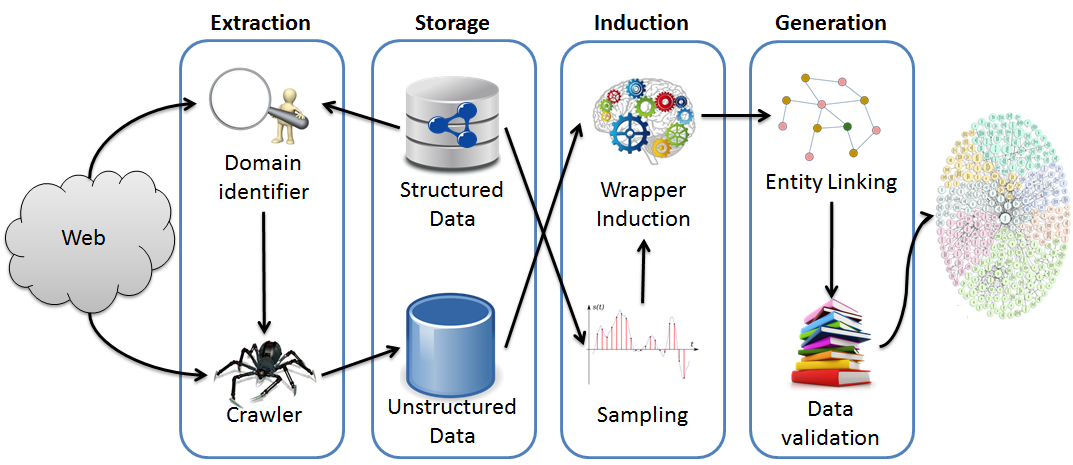
\includegraphics[width = \textwidth]{part_02/semi_structured_annotation/ISWC_REX/rexArchitecture}
\caption{Architecture of REX.}
\label{charex:fig:architecture}
\end{figure}
\subsection{Extraction Layer}
REX's data extraction layer consists of two main components:
The \emph{domain identification module} is the first component of the layer and takes a set of triples $(s, p, o)$ as examples and returns a ranked list of Web domains.
Our current implementation simply uses the Google interface to search for websites that contain the label of all $s$, $p$ and $o$.
The top-10 domains for each triple are selected and their rank is averaged over all triples.
The resulting ranking is returned. 
Moreover, we provide a manual domain identification module for expert users.
For our example \texttt{dbo:actor}, we get \url{http://imdb.com} as top-ranked domain.
The second component consists of a \emph{crawler interface} which allows to gather the Web pages that are part of the detected domain and collect them in a storage solution for unstructured data.
Currently, we rely on crawler4j\footnote{\url{https://code.google.com/p/crawler4j/}} for crawling and Apache Lucene\footnote{\url{http://lucene.apache.org/}} for storing the results of the crawling.  

\subsection{Storage Layer}
The storage layer encapsulates the storage solutions for structured data (i.e., the  \ac{KB} $K$) and the unstructured data (i.e., the output of the extraction layer). 
We assume that the structured data can be access via SPARQL.
The unstructured data storage is expected to return data when presented with a pair $(s, o)$ of resources, which is commonly a positive or negative example for the pairs that abide by $p$.
As stated above, we rely on a Lucene index that can access the labels of resources and simply search through its index for pages that contain both a label for $s$ and a label for $o$.

\subsection{Induction Layer}
The induction layer uses the data in the storage layer to compute wrappers for the website crawled in the first step.
To this end, it contains two types of modules:
The \emph{example generation} module implements sampling algorithms that are used to retrieve examples of relevant pairs $(s, o)$ such that $(s, p, o) \in K$. 
These examples are used to feed the \emph{wrapper induction} module, which learns the wrappers that are finally used to extract data from Web pages.
Hereafter, we present the implementations of these modules.

\subsubsection{Generation of Examples}
Given a  \ac{KB} $K$, the generation of all examples $\examples$ for a predicate $p$ can be retrieved by computing all triples $<s,p,o>$ from $K$.
However, using all triples might lead to poor scalability, especially if $K$ is very large.
To ensure the scalability of our approach, we thus aimed to ensure that we can provide REX with only a sample of $\examples$ and thus reduce its learning runtime without diminishing its accuracy.  
Our first intuition was that it is more likely to find resources that stand for well-known real-world entities on the Web. 
Thus, by selecting the most prominent examples from the knowledge $K$, we should be able to improve the probability of finding Web pages that contain both the subject and the object of our examples. 
This intuition can be regarded as prominence-driven, as it tries to maximize the number of annotated pages used for learning. 
We implemented this intuition to generating a sample of $\examples$ by implementing a first version of the example generator that ranks the examples $(s, o)$ in $\examples$ in descending order by how prominent they are in the  \ac{KB}. The score $scr$ for ranking the examples was computed by summing up the in- and out-degree of $s$ and $o$:
\begin{equation}
scr(s, o) = in(s) + in(o) + out(s) + out(o).
\end{equation}
We call this example selection \emph{prominence-based}.

The main drawback of this first intuition is that it introduces a skew in the sampling as we only consider a subset of entities with a particular distribution across the pages in $W$. 
For example, actors in IMDB have different templates depending on how popular they are. 
Learning only from popular actors would then lead to learning how to extract values only from Web pages obeying to particular type of HTML template. 
%Thus, as our experiments show, while this approach achieves a high recall when looking for web pages, it can lead to incorrect wrappers if only a small subset of $P$ is selected for learning.
%maybe we should write here that the correction of this bias is carried out by the learning appraoch?
While this problem can be by choosing a large number of examples, we revised our sampling approach to still use the ranking but to sample evenly across the whole list of ranked resources. 
To this end, given a number $n$ of required pairs, we return the first $n$ pairs $(s,o)$ from the ranked list computed above whose index $idx$ abides by:
\begin{equation}
idx(s, o) \equiv 0  \left(mod\left \lfloor{\frac{|\examples|}{n}}\right \rfloor \right).
\end{equation}
We call this second implementation of the example generator interface the \emph{uniform} approach .
%By these means, we can ensure that the whole of the distribution of resource prominence is covered by our approach. Consequently, we can support the generation of robust wrappers from the given input data.

%\paragraph{Negative Examples}
%Although it's sufficient to restrict to positive examples only, the usage of negative examples can help to improve the \emph{wrapper induction} step by reducing the hypothesis space. Assuming that we have a positive example $<s,p,o>$ and $dom(p)$(resp. $ran(p)$) denotes the domain (resp. range) of $p$, we generate negative examples as follows:
%\begin{itemize}
%\item Generate a new triple $<s',p,o>$ where $s'$ is an instance of $dom(p)$ and $<s',p,o>$ does not exist in $K$.
%\item Generate a new triple $<s,p,o'>$ where $o'$ is an instance of $ran(p)$ and $<s,p,o'>$ does not exist in $K$.
%\item Generate a new triple $<s',p,o'>$ where $s'$ is an instance of $dom(p)$, $o'$ is an instance of $ran(p)$ and $<s',p,o'>$ does not exist in $K$.
%\end{itemize}


\subsubsection{Wrapper Generation} %(DQ, VC, PM)
\label{alfred}
%- Several approaches in the literature to generate wrappers
%Several years of reasearch on data extraction from web pages have produced a large number of proposals for producing web wrappers (see~\cite{} for a survey). 

% START: alfred commands (Disheng)
\newcommand{\xpath}[1]{\mbox{\sf\small #1}}
%\newcommand{\htmlvalue}[1]{\mbox{\tt\small #1}}
\newcommand{\htmlvalue}[1]{\mbox{`#1'}}
\newcommand{\lc}[2]{\mbox{\ensuremath{LC(#1,#2)}}}%% local consistency
\newcommand{\gc}[2]{\mbox{\ensuremath{Sep(#1,#2)}}}%% global  consistency- separable now!

\newcommand{\allpages}{\mbox{\ensuremath{W}}}
\newcommand{\somepages}{\mbox{\ensuremath{Q}}}
\newcommand{\innersamples}{\mbox{\ensuremath{I}}}
\newcommand{\csample}{\mbox{\ensuremath{C}}}
\newcommand{\nil}[1]{\mbox{\ensuremath{nil_{}}}}
\newcommand{\accr}[1]{\mbox{\ensuremath{Acc(#1)}}}
\newcommand{\vect}[1]{\overrightarrow{#1}}
\newcommand{\rules}{\ensuremath{R}}
\newcommand{\allvects}{\ensuremath{\mathcal{V}^U}}
\newcommand{\allrules}{\ensuremath{\mathcal{R}}}
\newcommand{\nonallrules}{\ensuremath{\overline{\mathcal{R}}}}
\newcommand{\nonammrules}[1]{\ensuremath{\overline{\mathcal{R}}_{#1}}}
\newcommand{\ammvect}[1]{\ensuremath{V_{#1}}}
\newcommand{\ammrule}[1]{\ensuremath{R_{#1}}}
\newcommand{\nonammvect}[1]{\ensuremath{\overline{V}}_{#1}}
\newcommand{\allammrules}[1]{\ensuremath{\mathcal{R}_{#1}}}
\newcommand{\allammvalues}[2]{\ensuremath{\widehat{V}^{#1}_{#2}}}
\newcommand{\queryablevalues}[2]{\ensuremath{V^{#1}_{#2}}(U)}
\newcommand{\lqueryablevalues}[3]{\ensuremath{V^{#1}(#2,#3)}}
\newcommand{\ltypedqueryablevalues}[4]{\ensuremath{V_{#1}^{#2}(#3,#4)}}
\newcommand{\typedqueryablevalues}[2]{\ensuremath{V_{#1}(#2)}}
\newcommand{\equivalence}[1]{\ensuremath{Eq_{U}(#1)}}

\newcommand{\lessexpressive}[1]{\ensuremath{Exp_{min}{(#1)}}}
\newcommand{\equivalencerules}[3]{\ensuremath{Eq^{#3}(#1,#2)}}

\newcommand{\subtypeof}{\ensuremath{\subseteq}}
\newcommand{\supertypeof}{\ensuremath{\supseteq}}

\newcommand{\mq}{\mbox{\em MQ}}
\newcommand{\alf}{\mbox{\sc alf}}
\newcommand{\alfrex}{\mbox{\sc AlfREX}}
\newcommand{\sampler}{{\sc Page\-Sampler}}
\newcommand{\page}{\mbox{\em w}}
\newcommand{\att}[1]{\mbox{\sf #1}}
\newcommand{\val}[1]{{\mbox{\sf '#1'}}}
\newcommand{\valm}[1]{\mbox{\sf #1}}
\newcommand{\abs}[2]{\mbox{\sf abs(#1,#2)}}
\newcommand{\rel}[2]{\mbox{\sf #1(`#2')}}
%\newcommand{\lab}[1]{\mbox{\ensuremath{l(#1)}}}

\newcommand{\alg}[1]{{\sc #1}}
\newcommand{\scegliDomanda}{\textsc{choose\-Question}}
\newcommand{\terminaAlgoritmo}{\mbox{\textsc{halt}}}
\newcommand{\espandiBacinoRegoleCandidate}{\textsc{expandRuleSet}}
\newcommand{\leggiRisposta}{\mbox{\textsc{oracle}}}

\newcommand{\type}[1]{\mbox{\em \ensuremath{#1}}}

\newcommand{\dalvi}{DBLP:journals/pvldb/DalviKS11}
\newcommand{\mdl}{DBLP:journals/corr/math-ST-0406077}
\newcommand{\lixto}{DBLP:conf/pods/GottlobKBHF04}
\newcommand{\angluin}{DBLP:journals/tcs/Angluin04}
\newcommand{\myjacm}{DBLP:journals/jacm/CrescenziM04}
\newcommand{\SL}{DBLP:journals/tnn/Vapnik99}
\newcommand{\srm}{DBLP:journals/tit/Shawe-TaylorBWA98}
\newcommand{\ALsurvey}{settles.tr09}

%\newtheorem{example}{Example}

% END %

%\section{Wrapper Generation}
Detecting rules to extract the subject-object pairs related to a property $p$ is the most difficult step when aiming to extract \ac{RDF} from templated website.
Here, we present our current implementation of the wrapper induction module interface of REX, which aims to extract subject-object pairs for $p$ from a set of pages $\allpages$ that belong to the same website and share a common template.
We assume that an \emph{example generator} provides the input set ${\examples}$ containing a subset of the pairs that can be extracted from the pages in $\allpages$. 
Formally,  let $\somepages$ denote the set of pages that contain a pair in $\examples$:
\begin{equation}
 \somepages = \{\page: \page \in \allpages,\ (s, o)\in {\examples} \wedge (\lab{s},\lab{o}) \in\ \page\},
\end{equation}
where  $(\lab{s},\lab{o}) \in \page$ denotes that at least one of the labels of $s$ and at least one of the labels of $o$ occur in the page $\page$. %In other words, 
We use the pairs in ${\examples}$ to gain the positive annotations for the pages in $\somepages$. These  annotations are needed to automatically infer a set of wrappers, i.e., a set of extraction rule pairs that extract the target subject-object pairs.

%Inferring a wrapper from a large number of annotations increases the computational costs. On the other hand, 
%the accuracy of the generated wrappers strongly depends on the number of training annotations used in the inference process.
%With a small number of annotations, the generated wrappers could be biased towards the variants of the HTML template observable in the sampled pages. For example, if the triples in $\somepages$ are all about famous actors, it might be the case that the inferred rules do not work on pages related to less popular actors in $\allpages$, since these pages could obey a slightly different variant of the template without some fields such as the prizes won, the user comments, etc. etc.

%We introduce a technique that first generate a set of wrappers %starting from a small set of annotations to reduce the costs, and %then rank the wrappers' rules using all the pairs extracted from %$\somepages$ to cover a large
%number of template variants.


% in alternativa alcuni sistemi supervisionati come ALF possono migliorare e certificare la qualità
% la copertura delle regole inferite
To avoid the extraction of incorrect values, our approach includes a technique to evaluate the output wrapper coverage, i.e., the number of pages in {\allpages} for which the wrappers inferred from {\somepages} correctly extract the target subject-object pairs. 

%\subsubsection{Learning Web Wrappers}
%\label{sec:learning-wrappers}

Listing~\ref{lst:learning-wrappers} reports the pseudo-code of our algorithm to generate the wrappers that extract subject-object pairs related to a property $p$ from a set of pages: 
%
it takes as input the set of pages $\allpages$ and the set of examples ${\examples}$.
%, i.e., the pairs $(s,o)$ generated by the previous component, the \emph{example generator}. 
To abstract the extraction rules generative process in our implementation, we assume that there exists, as a parameter of the algorithm, a class of all the creatable extraction rules $\allrules$. It corresponds to the set of XPath expressions that we can generate over the pages in \allpages.

\begin{algorithm}[htb!]
\caption{{\alfrex}: Extract subject-object pairs from a website.}\label{lst:learning-wrappers}
\label{alg:alfrex}
\begin{algorithmic}[1]
\renewcommand{\algorithmicensure}{\textbf{Output:}}
\newcommand{\LET}{\mbox{\textbf{let}}}
\renewcommand{\algorithmicrequire}{\textbf{Input:}}
\REQUIRE \ac{KB} $K$, a predicate $p$, a set of examples $\examples = \{(s,o)|(s,p,o) \in K\}$
\REQUIRE a set of pages $\allpages=\{w_1,\ldots,w_{|\allpages|}\}$ containing data w.r.t. predicate $p$

\renewcommand{\algorithmicrequire}{\textbf{Parameter:}}
\REQUIRE a class of extraction rules $\allrules$ over $\allpages$
\REQUIRE $k$, the number of sample pages for generating the rules

\ENSURE set $T$ of pairs of strings extracted from pages $W$
\bigskip
\STATE $T := \emptyset$; {\em // output pairs of strings}
\STATE $Q := \{\page \in \allpages$: $(\lab{s},\lab{o}) \in \page$, $ (s, o) \in \examples\};$\label{lst:Q}
\STATE $I :=$ a set of $k$ random pages from $Q$;\label{lst:I}
\STATE $R_s := \{r, r \in \allrules, \page \in I, (\lab{s}, \lab{o}) \in \page, r(\page) = \lab{s}\}$;\label{lst:Rs}
\STATE $R_o := \{r, r \in \allrules, \page \in I, (\lab{s}, \lab{o}) \in \page, r(\page) = \lab{o}\}$;\label{lst:Ro}
\STATE $(r_s, r_o) := \argmax_{r_s\in R_s, r_o \in R_o}$~~$|\{\page, \page \in Q, (\lab{s},\lab{o}) \in \page,$\\$ r_s(q) = \lab{s}\ \AND\ r_o(q) = \lab{o}\}|$;\label{lst:best-pair}
\STATE $\{r_s^1,r_s^2,\ldots, r_s^n\} \leftarrow \{r, r \in R_s, r(Q)=r_s(Q) \}$;\label{lst:best-vector-s}
\STATE $\{r_o^1,r_o^2,\ldots, r_o^m\} \leftarrow \{r, r \in R_o, r(Q)=r_o(Q) \}$;\label{lst:best-vector-o}

\FOR{$q\in \allpages$}\label{lst:forall-start}
    \IF {($r_s^1(q)=\ldots=r_s^n(q)\ \AND\ r_o^1(q)=\ldots=r_o^m(q)$)}\label{lst:check}
    \STATE $T \leftarrow T \cup \{(r_s^1(q),r_o^1(q))\}$;
    \ENDIF
\ENDFOR\label{lst:forall-end}

\RETURN $T$;

\end{algorithmic}
\end{algorithm}


As a first step (line~\ref{lst:Q}), the algorithm computes the set of pages $Q$
(we assume $Q \neq \emptyset$).
Then, it picks up a small set of sample pages $I$ from $Q$.%
In our implementation, we set $k = |I| = 10$.
%
From the pages in $I$ two initial sets of extraction rules, $R_s$ and $R_o$, are generated (lines~\ref{lst:Rs}-\ref{lst:Ro}), as follows. 
%
%
First, we analyze the DOM tree of the pages to locate nodes that are part 
of the template. We use these nodes as roots of XPath expressions that 
match with the input pair. To discover the template nodes, we compute the occurrences of the textual leaf nodes in the pages. Following the intuition developed in~\cite{exalg}, 
we consider template nodes the document root, the nodes with an {\em id} attribute, 
and  the text leaves that occur exactly once  with same value and same root-to-leaf sequence of tags in a significant 
percentage (80\%) of pages.  The rationale is that it is very unlikely that a node occurs exactly once in several pages with the same root-to-leaf path by chance; rather, it is likely repeated  in every page since it comes from a piece of the underlying HTML template.

Template nodes are then used as {\em pivot nodes} to generate XPath expressions that 
match with nodes containing a textual leaf that equals the subject (object) of the 
input pair. Given a pivot node $l$, an XPath expression for the textual node $t$ 
is computed by appending three expressions: $(i)$~an expression that matches with the
pivot node $t$, $(ii)$~the path from $t$ to the first ancestor node,
$n_{lt}$, shared by $t$ and $l$, $(iii)$~the path from $n_{lt}$ to $l$ 
(which descends from the shared ancestor node to the target textual node).
To avoid an excessive proliferation of rules, we bound the length of
the XPath expressions, i.e., the number of XPath steps.
We observed that producing rules longer than 8 steps do not produce any benefit.

\begin{figure*}[htb]
\newcommand{\sxpath}[1]{\xpath{\scriptsize#1}}
\begin{tabular}{ccc}
\multicolumn{3}{c}{
\vspace{0pt}
    \resizebox{0.95\textwidth}{!}{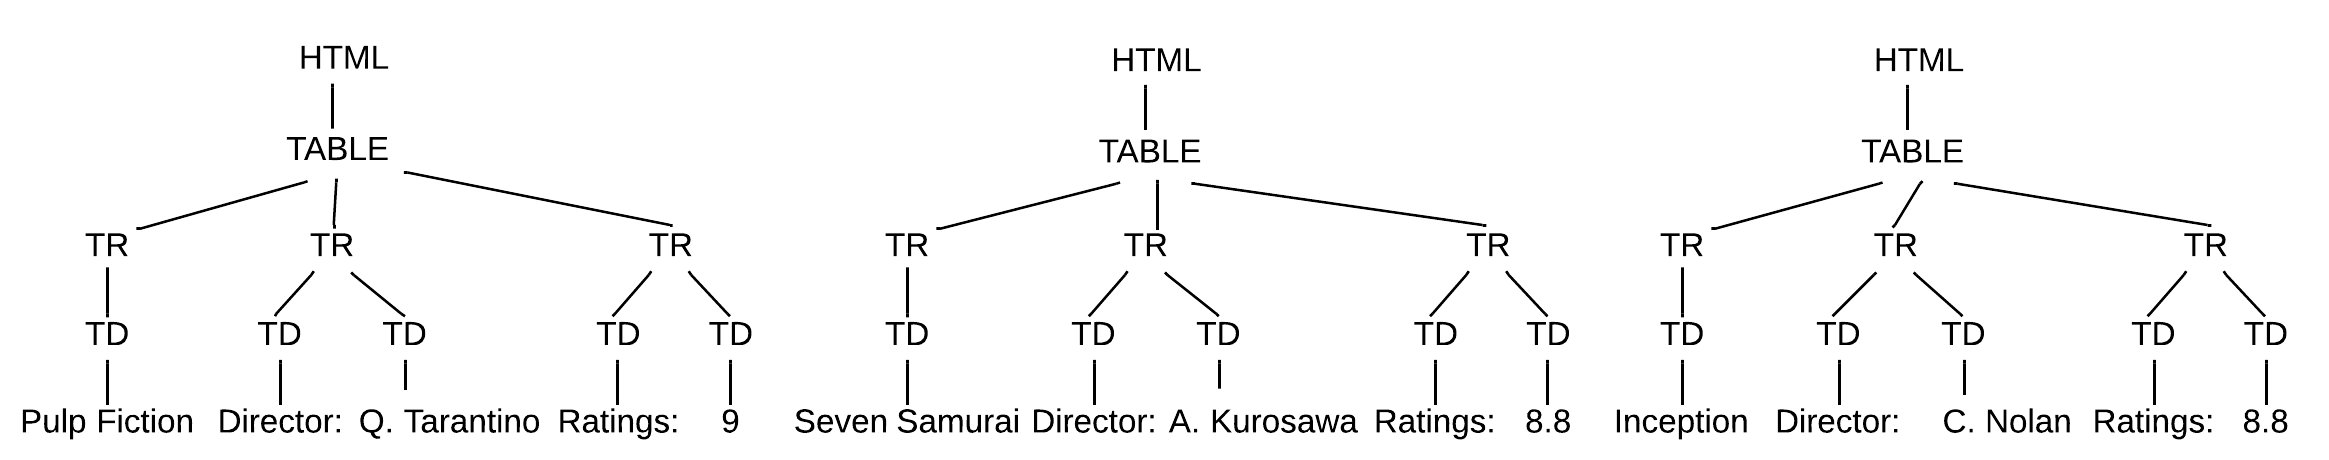
\psfig{file=part_02/semi_structured_annotation/ISWC_REX/dom-I.png}}
}\\
%
\multicolumn{3}{c}{\bf (a)}\\
%
\multicolumn{1}{c}{
    \resizebox{0.2\textwidth}{!}{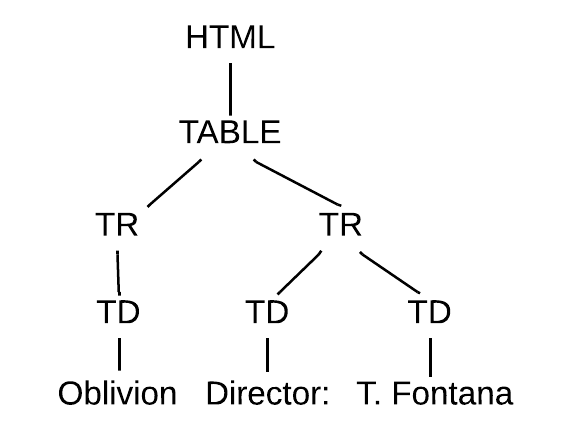
\psfig{file=part_02/semi_structured_annotation/ISWC_REX/dom-Q.png}} 
} &
\multicolumn{1}{@{}c@{}}{
    \raisebox{0.5\totalheight}{
    \scalebox{0.85}{
\begin{tabular}{@{}r@{:~}l@{}}
\multicolumn{2}{l}{\em Extraction rules}\\
$r^1$  & {\sxpath{//*[contains(.,"Ratings:")]/../p-s::tr[2]/td/text()
}}\\
$r^2$  & {\sxpath{//*[contains(.,"Director:")]/../p-s::tr[1]/td/text()
}}\\
$r^3$  & {\sxpath{/html/table/tr[1]/td/text()}}\\
\multicolumn{2}{l}{\em ps = preceding-siblings} \\
\end{tabular}}}}  &
\vspace{0pt}
    \resizebox{0.35\textwidth}{!}{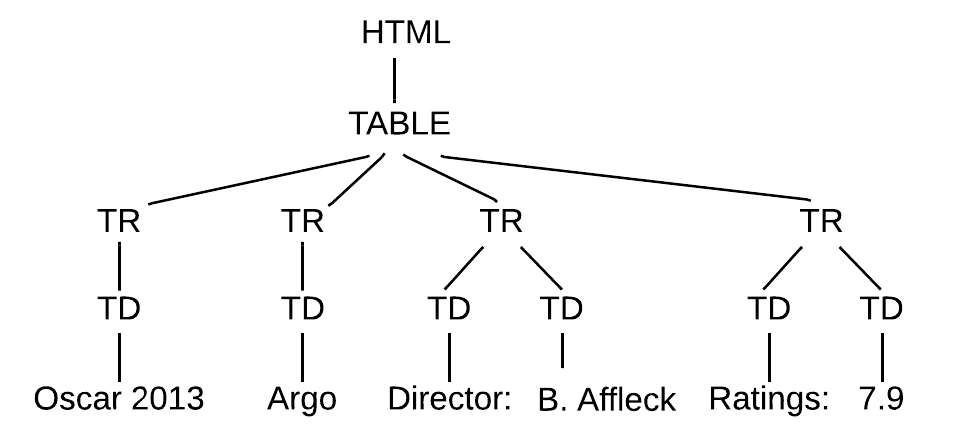
\psfig{file=part_02/semi_structured_annotation/ISWC_REX/dom-W.png}} \\
%
\multicolumn{1}{c}{\bf (b)} & \multicolumn{1}{c}{\bf (c)} & \multicolumn{1}{c}{\bf (d)} 
\\
\end{tabular}
 \caption{%
 {\bf (a)} DOM trees of three pages (in a fictional set $I$), 
 {\bf (b)} a page in $Q$ (with a template that differs from those of the pages in $I$), 
 {\bf (c)} some rules to extract the movie title, and
 {\bf (d)} a page in $W$ (with a template that differs from those of the pages in $Q$).}%
 \label{fig:dom-trees}
\end{figure*}


The above step produces several extraction rules that correctly work on the pages 
in $I$. However some of these rules could not work on a larger set of pages. 
For example, consider a set of pages such as those shown in Figure~\ref{fig:dom-trees} (a). Assuming that the leaf nodes {\htmlvalue{Director:}} and {\htmlvalue{Ratings:}} appear once with the same root-to-leaf path in most of the pages in $I$, they would be considered as template nodes. Figure~\ref{fig:dom-trees} (c) reports an example of the XPath expressions pivoted in these nodes, and generated to extract the movie title.
%
%\end{example} 
%
Notice, however, that rule $r^1$ does not extract the movie title on pages like that depicted in Figure~\ref{fig:dom-trees} (b), i.e., pages without user ratings.
To improve the accuracy of the rules generated from pages in $I$, we evaluate the generated rules over $Q$, and select those that extract the largest number of annotations (line~\ref{lst:best-pair}). In our example, the extraction rules $r^2$ and $r^3$ would be selected, while $r^1$ would be discarded, as the former rules work also on the page of Figure~\ref{fig:dom-trees} (b), while the latter does not. 

%\floatname{algorithm}{Listing}



The selected rules are those better working for the pages in $Q$, that are the pages containing pairs of $K$. Although it is likely that these rules also work for the whole collection of input pages, it might also be the case that {\allpages} contains pages obeying to a slightly different template not observed within $Q$. For example, consider the page in Figure~\ref{fig:dom-trees} (d): since the movie has been awarded 3 Oscars, the corresponding page has small structural differences, and neither $r^1$ nor $r^3$ correctly extract the title. 


To overcome this issue, we leverage the redundancy of equivalent rules generated in the above steps. Targeting only resources from pages for which the extraction is likely to work correctly, we return the pairs (lines~\ref{lst:best-vector-s}-\ref{lst:best-vector-o}) on which all the distinct yet equivalent rules return the same value. Again from our example, observe that rules $r^2$ and $r^3$ extract different values from the page in Figure~\ref{fig:dom-trees} (d) ({\em Argo} and {\em Oscar 2013}, respectively), therefore, none of the values extracted from that page would be added in the final output. 
%{\bf DQ: cosi funziona? :)}
%{\bf DA SISTEMARE. ATTENZIONE: L'ESEMPIO NON FUNZIONA LE DUE REGOLE SI COMPORTANO ALLO STESSO MODO}
All these rules are used later (lines~\ref{lst:forall-start}-\ref{lst:forall-end}) to check that they extract the same value (line~\ref{lst:check}) from a web page.


%We could also rely to other supervised systems (such as~\cite{DBLP:conf/www/CrescenziMQ13a}) to further improve and guarantee the quality and the coverage of the extraction rules.



\subsection{Generation Layer}
Now that data has been extracted from the websites, REX is ready to generate \ac{RDF} out of them. 
To achieve this goal, two steps needs to be carried out. 
First, the strings retrieved have to be mapped to \ac{RDF} resources or literals. 
This is carried out by the \emph{URI disambiguation} modules. 
The resulting triples then need to be checked for whether they go against the ontology of the  \ac{KB} or other consistency rules. 
This functionality is implemented in the \emph{data validation} modules. 

\subsubsection{URI Disambiguation}\label{urigen}
%Subsequently to generating the best possible wrapper for a domain of a property $p$ we need to generate triples from each pair $(s, o) \in T$.
%To achieve this goal, we try to match $(s,o)$ against resources from the knowledge base $K$.
URI disambiguation is not a trivial task, as several resources can share the same label in a  \ac{KB}. 
For example, ``Brad Pitt'' can be mapped to the resource \texttt{:Brad\_Pitt} (the movie star) or \texttt{:Brad\_Pitt\_(boxer)}, an Australian boxer. 
We address this problem by using \emph{AGDISTIS}, a framework for URI disambiguation~\cite{agdistis_iswc}.
In our current implementation, we chose to simply integrate the AGDISTIS framework using DBpedia 3.8.
We chose this framework because it outperforms the state-of-the-art frameworks AIDA~\cite{AIDA} and DBpedia Spotlight~\cite{spotlight} by 20\% w.r.t. its accuracy. 
Especially on short RSS feeds containing only two resource labels, the approach achieves 3\%  to 11\% higher accuracy. 
More details on AGDISTIS as well as a thorough evaluation against popular frameworks such as DBpedia Spotlight and AIDA can be found in~\cite{agdistis_iswc}.
Note that if no resources in $K$ has a URI which matches $s$ or $o$, we generate a new cool URI\footnote{\url{http://www.w3.org/TR/cooluris}} for this string.% following the DBpedia guidelines~\cite{DBLP:conf/semweb/AuerBKLCI07}.

\subsubsection{Data Validation}\label{axioms}
Sequentially applying the steps before results in a set of triples $<s,p,o>$ that might not be contained in $K$. 
As we assume that we start from a consistent  \ac{KB} $K$ and the whole triple generation process until here is carried out automatically, we need to ensure that $K$ remains consistent after adding $<s,p,o>$ to $K$.
To this end, REX provides a data validation interface whose first implementation was based on the DL-Learner.\footnote{\url{http://dl-learner.org}}
Depending on the size of $K$, using a standard OWL reasoner for consistency checks can be intractable.
%\todo[inline]{@Lorenz: Citation for the claim pls}
Thus, our current implementation applies the following set of rules based on the schema of $K$ and add a triple $<s_1,p,o_1>$ only if it holds that:
\begin{enumerate}
\item If a class $C$ is the domain of $p$, there exists no type $D$ of $s_1$ such that $C$ and $D$ are disjoint.
\item If a class $C$ is the range of $p$, there exists no type $D$ of $o_1$ such that $C$ and $D$ are disjoint.
\item If $p$ is declared to be functional, there exists no triple $<s_1,p,o_2>$ in $K$ such that $o_1 \neq o_2$.
\item If $p$ is declared to be inverse functional, there exists no triple $<s_2,p,o_1>$ in $K$ such that $s_1 \neq s_2$.
\item If $p$ is declared to be asymmetric, there exists no triple $<o_1,p,s_1>$ in $K$.
\item If $p$ is declared to be irreflexive, it holds that $s_1 \neq o_1$.
\end{enumerate}
Note that this approach is sound but of course incomplete.
Although an increasing number of \ac{RDF}  \ac{KB}s are published, many of those consist primarily of instance data and lack sophisticated schemata. 
To support the application of the above defined rules, we follow the work in \cite{buhmann2012,pattern_enrichment}, which provides a lightweight and efficient schema creation approach that scales to large  \ac{KB}s. 
%The creation of the (extended) schema is done in three steps:

%\begin{enumerate}
%\item In the optional first step, SPARQL queries are used to obtain existing information about the schema of the  \ac{KB}, in particular we retrieve axioms which allow to construct the class hierarchy. Naturally, the schema only needs to be obtained once per  \ac{KB} and can then be re-used by all algorithms and all entities.
%\item The second step consists of obtaining all the data via SPARQL, which is relevant for learning the considered axiom.
%This results in a set of axiom candidates.
%\item In the third step, the score of axiom candidates is computed and the results returned.
%\end{enumerate}

%Suppose we want to search for the domain of $p$ and got a class $A$ as possible candidate from step 2, then we have to run 3 SPARQL queries to obtain all data for computing the score by means of precision and recall: one query for the number of instances having at least one $p$ ($|\exists p.\top|$), one for the instance count of $A$ ($|A|)$, and another one to get the number of instances contained in the intersection of both ($|\exists p.\top \sqcap A|$).
%Based on that information, we can compute precision $P$ as $P=\frac{|\exists p.\top \sqcap A|}{|A|}$ and recall $R$ as $R=\frac{|\exists p.\top \sqcap A|}{|\exists p.\top|}$, both resulting in a total score for  $A$  being the domain of $p$ using standard F-measure.

%A disadvantage of using this straightforward method of obtaining a score is that it does not take the \emph{support} for an axiom in the  \ac{KB} into account. 
%Specifically, there would be no difference between having 100 out of 100 correct observations or 3 out of 3 correct observations when computing precision and recall.
%For this reason, we do not just consider the count, but the average of the 95\% confidence interval of the count.
%This confidence interval can be computed efficiently by using the improved Wald method defined in~\cite{approx}. 
%Assume we have $\mu$ observations out of which $\sigma$ were successful, then the approximation of the 95\% confidence interval is as follows:

%\begin{scriptsize}
%\[
%\left[
% \max(0, p' - 1.96 \cdot \sqrt{\frac{p' \cdot (1-p')}{\mu+4}}) , %\textnormal{ to }
% \min(1, p' + 1.96 \cdot \sqrt{\frac{p' \cdot (1-p')}{\mu+4}}) 
%\right]
%\]
%\end{scriptsize}

%\noindent
%with $p' = \frac{\sigma+2}{\mu+4}$.
%This formula is easy to compute and has been shown to be accurate in~\cite{approx}.
%This step concludes the extraction of RDF triples from websites.

\section{Evaluation}
\label{sec:evaluation}
The goal of the evaluation was to provide a detailed study of the behavior of the current REX modules with the aim of (1) ensuring that our framework can be used even in its current version and (2) detecting current weaknesses of our framework to trigger future developments.
In the following, we begin by presenting the data and hardware we used for our experiments. 
Thereafter, we present and discuss the results of our experiments.
Detailed results can be found at the project website.

%\begin{enumerate}

%\item We wanted to determine the amount of knowledge that we need to learn sensible pairs of XPath expressions. We thus provided our wrapper inference component with a variable number of examples and measured the influence of the number of examples on the overall F-measure of our approach. 
%%\item We also wanted to evaluate how well our approach can estimate its own confidence in the expressions it learned. We thus conducted a series of experiments where we measured the change in sure of our approach with varying confidence thresholds.
%\item To measure the runtime performance of our approach, we measured the amount of time that REX required to learn  wrappers from the input data. Especially, we measures the influence of the size of $I$ on the runtime of REX as well as on the average F-measure achieved by our approach. 
%\item Finally, we wanted to measure the quality of the end result of our approach, i.e., the quality of the output RDF. We thus sampled the triples generated by our approach and approximated its overall accuracy. 
%\end{enumerate}
 
\subsection{Experimental Setup}
We generated our experimental data by crawling three websites, i.e., 
\begin{enumerate}
\item \url{imdb.com} where we extracted \url{dbo:starring}, \url{dbo:starring}$^{-1}$ as well as \url{dbo:director};
\item \url{goodreads.com}, from which we extracted \url{dbo:author} and \url{dbo:author}$^{-1}$;
\item \url{espnfc.com} with the target relations \url{dbo:team} and \url{dbo:team}$^{-1}$.
\end{enumerate}
%For each website, we focused on two subdomains (see~Table~\ref{tab:dataset}). 
We chose these websites because they represent three different categories of templated websites.
\url{imdb.com} widely follows a uniform template for all pages in the same subdomain.
%Moreover, there are rarely any pages with missing values in this site.
Thus, we expected the wrapper learning  to work well here.
\url{goodreads.com} represents an average case of templated websites. 
While template are most widely used and followed, missing values and misused fields are more common here than in our first dataset.
%Thus, we assume that the values achieved on this dataset can be regarded as prototypical for our approach.
The third dataset, \url{espnfc.com}, was chosen as worst-case scenario.
The dataset contains several blank pages, a large variety of  templates used in manifold different fashions.
Consequently, defining a set of golden XPaths is a tedious task, even for trained experts.
Thus, we expected the results on this dataset to be typical for the worst-case behavior of our approach.
%Since all domains support incremental URLs we randomly sampled valid numbers in the respective range of valid URLs. 
We randomly sampled 10,000 HTML pages per subdomain for our experiments and manually built reference XPath expressions to evaluate the precision and recall of the generated extraction rules. 
The precision, recall and F-measure reported below were computed by comparing the output of REX with the output of the reference XPath expressions.
All extraction runtime experiments were carried out on single nodes of an Amazon EC2.small instance.

%\todo[inline]{State that some of the used properties are uni-directional}
%\todo[inline]{In the paper of \cite{Crescenzi2013} a much more sophisticated crawling strategy is described. We could engage this by stating that we crawl a much higher amount of data without loosing web-scalability}


%\begin{table}[htb]
%\centering
%\caption{Properties per dataset. \texttt{dbo} stands for \texttt{http://dbpedia.org/ontology/}.} 
%\label{tab:dataset}
%\begin{tabular}{lll}
%\toprule
%%\multicolumn{2}{c}{Domain}&Property\\
%%\midrule
%\multirow{2}{*}{\url{goodreads.com}} & Author   & \url{dbo:author}$^{-1}$\\
%                                     & Book     & \url{dbo:author} \\
%\midrule
%\multirow{2}{*}{\url{espnfc.com}}    & Team     & \url{dbo:team}$^{-1}$\\
%                                     & Player   & \url{dbo:team} \\
%\midrule
%\multirow{2}{*}{\url{imdb.com}}      & Actor    & \url{dbo:starring}$^{-1}$ \\
%                                     & Movie    & \url{dbo:starring} \\
%                                      & Movie    & \url{dbo:director} \\
%\bottomrule
%\end{tabular}
%\end{table}

\subsection{Results}
\paragraph{Effect of Number of Examples and Sampling Strategy on F-measure}


%\todo[inline]{RU: I think we need to define which f-measure was used here. AN: Done}
The results of our experiments on altering the number of examples used for learning are shown in Figures~\ref{charex:fig:pDirector}-\ref{charex:fig:uTeam}. 
Due to space limitations, we show the average results over all the pairs extraction by our wrapper induction approach for each of the domains.
The results achieved using the prominence-based sampling show the expected trend: on pages that use a consistent template (such as the director pages in \url{imdb.com}), our approach requires as few as around 70 pages for $|Q|$. 
Once this value is reached, REX can compute high-quality extraction rules and achieves an F-measure of 0.97 (see Figures~\ref{charex:fig:pDirector}).
For pages that change template based on the prominence of the entities they describe (like the actors' pages, see Figure~\ref{charex:fig:pActors}), our approach requires more training data to achieve a high F-measure.
The increase of F-measure is clearly due to an increase in precision, pointing to REX being able to better choose across different alternative XPaths when provided with more information.
The results of \url{goodreads.com} support our conjecture. 
With more training data, we get an increase in precision to up to 1 while the recall drops, leading to an overall F-measure of 0.89 for 40.000 examples.
In our worst-case scenario, we achieve an overall F-measure close to 0.6.
The lower value is clearly due to the inconsistent use of templates across the different pages in the subdomains.


\begin{figure}[htb!]
        \centering
        \subfloat[Directors from IMDB, prominence-based sampling.]{\label{charex:fig:pDirector}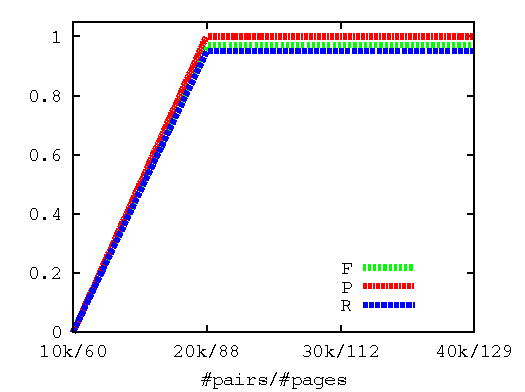
\includegraphics[width=.33\textwidth]{part_02/semi_structured_annotation/ISWC_REX/no-random-director.pdf}}~
        \subfloat[Actors from IMDB, prominence-based sampling.]{\label{charex:fig:pActors}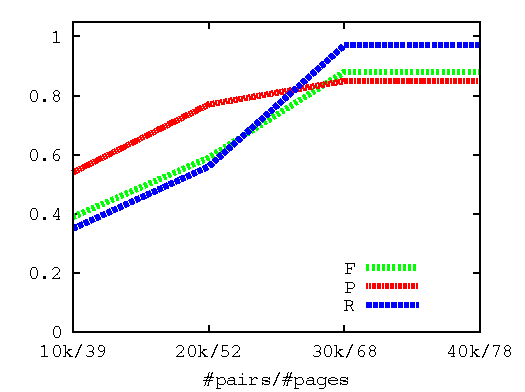
\includegraphics[width=.33\textwidth]{part_02/semi_structured_annotation/ISWC_REX/no-random-starring.pdf}}~
        \subfloat[Authors from Goodreads, prominence-based sampling.]{\label{charex:fig:pAuthor}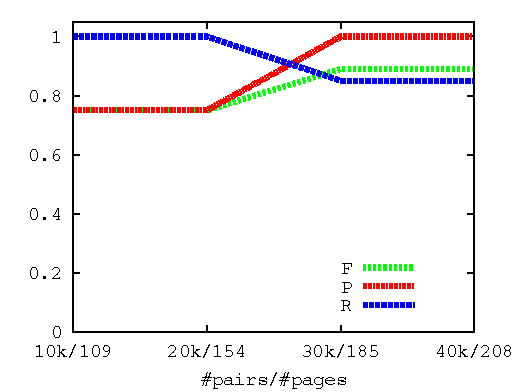
\includegraphics[width=.33\textwidth]{part_02/semi_structured_annotation/ISWC_REX/no-random-author.pdf}}

        \subfloat[Directors from IMDB, uniform sampling.]{\label{charex:fig:uDirector}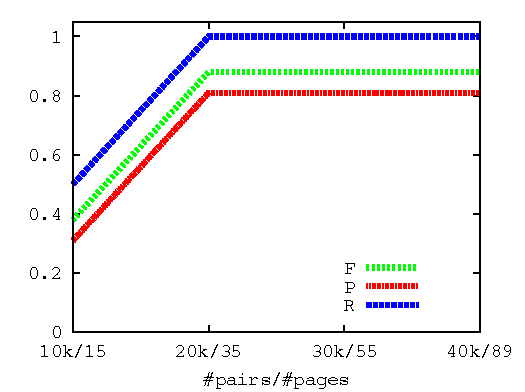
\includegraphics[width=.33\textwidth]{part_02/semi_structured_annotation/ISWC_REX/random-director.pdf}}~
        \subfloat[Actors from IMDB, uniform sampling.]{\label{charex:fig:uActors}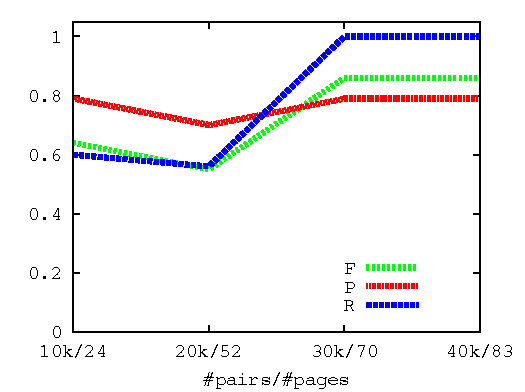
\includegraphics[width=.33\textwidth]{part_02/semi_structured_annotation/ISWC_REX/random-starring.pdf}}~
        \subfloat[Authors from Goodreads, uniform sampling.]{\label{charex:fig:uAuthor}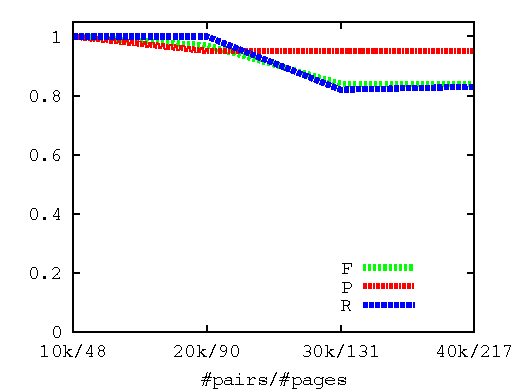
\includegraphics[width=.33\textwidth]{part_02/semi_structured_annotation/ISWC_REX/random-author.pdf}}
        
        \subfloat[Teams from ESPNFC, prominence-based sampling.]{\label{charex:fig:pTeam}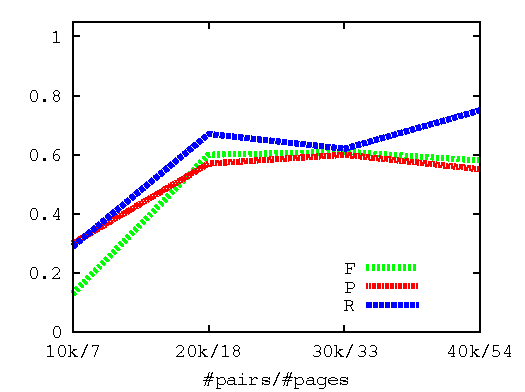
\includegraphics[width=.33\textwidth]{part_02/semi_structured_annotation/ISWC_REX/no-random-team.pdf}}~
        \subfloat[Teams from ESPNFC, uniform sampling.]{\label{charex:fig:uTeam}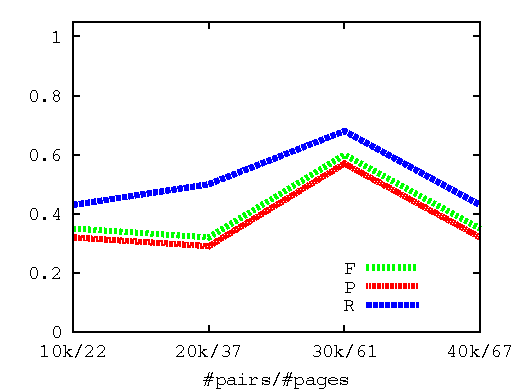
\includegraphics[width=.33\textwidth]{part_02/semi_structured_annotation/ISWC_REX/random-team.pdf}}~
        \subfloat[Average computational time and F-measure over all datasets.]{\label{charex:fig:runtime}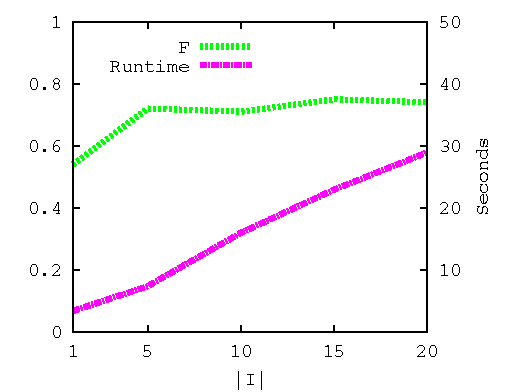
\includegraphics[width=.33\textwidth]{part_02/semi_structured_annotation/ISWC_REX/time-F.pdf}}
\caption[Overall evaluation results of REX]{Overall evaluation results of the extraction of pairs. Figures (a) to (h) show the average precision, recall and F-measure which is achiev\-ed by the generated XPaths for the prominence-based and uniform sampling. The x-axis shows the number of examples and the number of sample pages retrieved in the format $|E|$/$|Q|$. Figure (i) shows the average computational time and the corresponding F-measures for different sizes of $|I|$.}
\label{charex:fig:overall-XPaths}
\end{figure}


The results based on the uniform sampling strategy reveal another trait of REX. 
As expected, the coverage achieved using uniform sampling is clearly smaller in all cases. 
%Still, when a small number of examples $|E|$ is provided, the uniform sampling returns better results than the prominence-based sampling (compare results with $|E| = 10k$ on Figures~\ref{charex:fig:pDirector} and~\ref{charex:fig:uDirector}, Figures~\ref{charex:fig:pActors} and~\ref{charex:fig:uActors}, Figures~\ref{charex:fig:pAuthor} and~\ref{charex:fig:uAuthor} as well as Figures~\ref{charex:fig:pTeam} and~\ref{charex:fig:uTeam}) in all settings.  
%This is simply due to the examples selected by the uniform sampling better reflecting the different types of templates in the dataset.
%The main drawback of the uniform sampling strategy is that the instances it selects generally contain a larger percentage of erroneous resources than the data selected by the prominence-based sampling strategy.
%The effect of this larger percentage of erroneous resources increases when making use of larger sizes of uniformly %sampled examples $E$ if the fraction of pages with noisy data in $Q$ increases.
%With a larger percentage of noise in the training data, REX is then more prone to learn biased and sub-optimal XPath expressions, leading to the overall decrease of the F-measure of our system.
%The proportion of erroneous pages in the training data is yet different from dataset to dataset, leading to different patterns combing about across our experiments. For example, extracting teams already leads to more errors in the uniform sampling when $|E| = 20k$ while the precision remains superior for $|E| = 20k$ when extracting author data from \url{goodreads.com}. 
%Our observations led us to the following conclusions: When running (1) on a manually curated  \ac{KB} with only a small amount of erroneous data in the  \ac{KB} or (2) on a small number of examples $|E|$, the uniform distribution is to be preferred.
%However, when running on an automatically extracted  \ac{KB} or on a large set of examples, the prominence-based distribution should be used.
%An exact quantification of this behavior remains part of our future work.
The results achieved with all the training data available clearly show the importance of sampling, see Table~\ref{tab:overall}. 
While one could conjecture that using all data for training would be beneficial for our approach, the F-measures achieved by using all the data suggest that sampling can be beneficial for the extraction, especially when the Web pages do not follow a rigid template, e.g., in \url{esnpfc.com}, or when the data in the  \ac{KB} is noisy. 
Overall, our results suggest that our approach is accurate, also for pages where entities with different prominence are assigned variable templates as in \url{imdb.com} actors. 
If multiple occurrences of the same value are present in the same page (as in the case of books, actors and directors), our algorithm is able to detect the most stable one.
Moreover, our approach seems robust against noisy labels, even when there are many false positive in the page (e.g., book author pages that include many links to different books by the same author).
An important feature of our approach is that it can obtain accurate XPaths even by learning from a very small fraction of pages. 
For example, in our experiments on up to 40.000 pages, our approach learned XPath expressions from only 0.5\% to 1.16\% of $|W|$.
Still, for very noisy domains with an inconsistent use of templates, our approach can lead to less accurate extraction rules.
%, as shown by our results on the third dataset.
%Yet, manually crafting XPath expressions to extract these data is a very tedious task.
\begin{table}[htb]
\centering
\begin{tabular}{lcccc}
\toprule
  &  P & R & F-measure & \#Pages \\
\midrule
\url{dbo:director}  & 0.82 & 1.00 & 0.89 & 216\\
\url{dbo:starring}  & 0.86 & 1.00 & 0.90 & 316\\
\url{dbo:author}    & 0.94 & 0.85 & 0.86 & 217\\
\url{dbo:team}      & 0.32 & 0.43 & 0.35 & 656\\
\bottomrule
\end{tabular}
\caption{Average evaluation results using all available pairs as training data.} 
\label{tab:overall}
\end{table}

\paragraph{Runtime Performance}
We evaluated the runtime performance of our approach by using 40.000 examples and the prominence-based distribution while altering the size of $I$.
As expected, setting $|I|$ to a low value, e.g.,~1, leads to less rules being generated and thus to an overall better runtime performance, see~Figure~\ref{charex:fig:runtime}.
By setting $I$ to a low value, REX can be used to get a quick overview of possible extraction results, a
characteristic of our system that could result beneficial for end users.
Yet, it also leads to worse overall F-measures.
Setting $I$ to a higher value, e.g., 15, leads to a more thorough, i.e., more time-demanding, analysis of the websites and thus to better results. 
Still overall, our approach scales quasi linearly and requires on average less than thirty seconds to learn wrappers out of existing data even for $|I|=20$.

\paragraph{Quality of RDF Output}
To check the quality of the \ac{RDF} we generated, we manually checked the triples extracted from each property of our three domains.
Each triple was checked by at least two annotators, which reached a significant Kohen's kappa score~\cite{cohen1960coefficient} of 0.88 overall.
On \url{goodreads.com} we achieved a precision of 75.24\%.
While we achieve a precision of 78.85\% when extraction directors from \url{imdb.com} and of 75\% on \texttt{starring}, the extraction of \texttt{starring}$^{-1}$ proves more tedious (precision = 42.17\%).
As expected, the data extracted from \url{espnfc.com} has a low precision of 44.19\%.
The results on \texttt{starring}$^{-1}$ are due to the fact that several actors can star in a movie while assuming other roles. 
Thus, our extraction framework often overgenerates triples and produces false positives, e.g., directors are often included.
The results on \url{espnfc.com} are clearly due to the templates not being used correctly.
Still, our results clearly show the potential of our approach, as 60.68\% of the triples we extracted are both correct and novel, see Table~\ref{tab:rdfeval}.


\begin{table}[htb!]
\centering
\resizebox{\textwidth}{!}{ 
\begin{tabular}{lccccc}
\toprule
Property & \#Possible & \#Triples generated & \#Consistent & \#Correct & \#New   \\
 & triples   & by AlfREX& triples & triples & triples  \\
\midrule 
\url{dbo:author}$^{-1}$   & 54 & 32 & 32 & 22 & 22 \\% (67.7\%)\\
\url{dbo:author}          & 83 & 83 & 69 & 54 & 54 \\%(77.0\%)\\
\midrule 
\url{dbo:team}$^{-1}$     & 2  & 1  & 1  & 0  & 0  \\%(0\%)\\
\url{dbo:team}            & 30 & 55 & 42 & 19 & 13\\ %90 & 50 & ? & ? \\%(31.0\%) \\
\midrule 
\url{dbo:starring}$^{-1}$ & 40 & 99 & 83 & 35 & 34 \\%(42.7\%)\\
\url{dbo:starring}        & 70 & 70 & 44 & 33 & 32 \\%(73.9\%)\\
\midrule
\url{dbo:director}        & 61 & 56 & 52 & 41 & 41 \\%(78.8\%)\\
\bottomrule
\end{tabular} }
\caption{Triples generated by 100 randomly sampled pages, number of possible triples generated by using gold standard rules}
\label{tab:rdfeval}
\end{table}


\part{Question Answering on hybrid sources}
%\cleardoublepage
\ctparttext{
    The third part 
    INFORMATION GAP
}
%\documentclass{acm_proc_article-sp}

%\usepackage{url}
%\usepackage{graphicx}
%\usepackage{wrapfig}
%\usepackage{fancybox}
%%\usepackage{todonotes}
%\usepackage[disable]{todonotes}

%\usepackage{listings}

%\newtheorem{req}{Requirement}
%\newtheorem{definition}{Definition}
%\newtheorem{ex}{Example}

\newcommand{\code}[1]{\texttt{#1}}
%\newcommand{\eg}{e.g.,~}
%\newcommand{\ie}{i.e.,~}
%\newcommand{\Ie}{That is,~}
%\newcommand{\Eg}{For example,~}
% \newcommand{\url}[1]{\href{#1}{#1}}


\newcommand{\searchword}{family-friendly}
% \newcommand{\url}[1]{\href{#1}{#1}}

\newcommand{\placeholder}{\code{urn:placeholder}}
\newcommand{\placeholderB}{\code{urn:placeholder2}}

\hyphenation{me-thods}
\hyphenation{ori-gi-na-ting}
\hyphenation{sear-ching}
\hyphenation{func-tio-na-li-ties}


%\begin{document}
\lstset{language=Java}
\chapter{A Service-oriented Search Framework for Full Text, Geospatial and Semantic Search}
%
% You need the command \numberofauthors to handle the 'placement
% and alignment' of the authors beneath the title.
%
% For aesthetic reasons, we recommend 'three authors at a time'
% i.e. three 'name/affiliation blocks' be placed beneath the title.
%
% NOTE: You are NOT restricted in how many 'rows' of
% "name/affiliations" may appear. We just ask that you restrict
% the number of 'columns' to three.
%
% Because of the available 'opening page real-estate'
% we ask you to refrain from putting more than six authors
% (two rows with three columns) beneath the article title.
% More than six makes the first-page appear very cluttered indeed.
%
% Use the \alignauthor commands to handle the names
% and affiliations for an 'aesthetic maximum' of six authors.
% Add names, affiliations, addresses for
% the seventh etc. author(s) as the argument for the
% \additionalauthors command.
% These 'additional authors' will be output/set for you
% without further effort on your part as the last section in
% the body of your article BEFORE References or any Appendices.

%\numberofauthors{6} %  in this sample file, there are a *total*
% of EIGHT authors. SIX appear on the 'first-page' (for formatting
% reasons) and the remaining two appear in the \additionalauthors section.
%
%\newcommand{\unisterAddr}{
%       \affaddr{R\&D, Unister GmbH}\\
%    \affaddr{Barfussgaesschen 11}\\
%    \affaddr{Leipzig (Germany)}\\
%}
%\author{
% You can go ahead and credit any number of authors here,
% e.g. one 'row of three' or two rows (consisting of one row of three
% and a second row of one, two or three).
%
% The command \alignauthor (no curly braces needed) should
% precede each author name, affiliation/snail-mail address and
% e-mail address. Additionally, tag each line of
% affiliation/address with \affaddr, and tag the
% e-mail address with \email.
%
% 1st. author
%\alignauthor
%Andreas Both\\
%       \unisterAddr
%       \email{andreas.both@unister.de}
%% 2nd. author
%\alignauthor
%Axel-Cyrille Ngonga Ngomo\\
%       \affaddr{Universit\"at Leipzig, IFI/AKSW }\\
%%       \affaddr{Leipzig }\\
%       \affaddr{Leipzig (Germany)}\\
%       \email{ngonga@informatik.uni-leipzig.de}
% 3rd. author
%\alignauthor 
%Ricardo Usbeck\\
%       \affaddr{Universit\"at Leipzig, IFI/AKSW}\\
%       \affaddr{Unister GmbH, Leipzig}\\
%       \email{usbeck@informatik.\\uni-leipzig.de}
%\and  % use '\and' if you need 'another row' of author names
% 4th. author
%\alignauthor        
%Denis Lukovnikov\\
%       \affaddr{Universit\"at Leipzig, IFI/AKSW }\\
%       \affaddr{Leipzig }\\
%       \affaddr{Leipzig (Germany)}\\
%       \email{lukovnikov@informatik.uni-leipzig.de}
% 5th. author
%\alignauthor 
%Christiane Lemke\\
%       \unisterAddr
%       \email{christiane.lemke@unister.de}
% 6th. author
%\alignauthor 
%Maximilian Speicher\\
%       \affaddr{TU Chemnitz, VSR}\\
%       \affaddr{Unister GmbH, Leipzig}\\
%       \email{speim@hrz.tu-chemnitz.de}
  % use '\and' if you need 'another row' of author names
% 5th. author
%\alignauthor Sean Fogarty\\
%       \affaddr{NASA Ames Research Center}\\
%       \affaddr{Moffett Field}\\
%       \affaddr{California 94035}\\
%       \email{fogartys@amesres.org}
% 6th. author
%\alignauthor Charles Palmer\\
%       \affaddr{Palmer Research Laboratories}\\
%       \affaddr{8600 Datapoint Drive}\\
%       \affaddr{San Antonio, Texas 78229}\\
%       \email{cpalmer@prl.com}
%} % author
%\date{15 June 2014}
% Just remember to make sure that the TOTAL number of authors
% is the number that will appear on the first page PLUS the
% number that will appear in the \additionalauthors section.

%\maketitle
%\begin{abstract}
Over the last decade, a growing importance of search engines could be observed. 
An increasing amount of knowledge is exposed and connected within the Linked Open Data Cloud, which raises users' expectations to be able to search for any information that is directly or indirectly contained. 
However, diverse data types require tailored search functionalit\-ies\----such as semantic, geospatial and full text search. 

Hence, using only one data management system will not provide the required functionality at the expected level.
In this paper, we will describe search services that provide specific search functionality via a generalized interface inspired by RDF. 
In addition, we introduce an application layer on top of these services that enables to query them in a unified way. 
This allows for the implementation of a distributed search that leverages the identification of the optimal search service for each query and subquery.
This is achieved by connecting powerful tools like \textit{Openlink Virtuoso}, \textit{ElasticSearch} and \textit{PostGIS} within a single framework. 
%Finally, we will isolate the performance challenges.
%\end{abstract}
% A category with the (minimum) three required fields
%\category{TODO}{TODO}{TODO}
%A category including the fourth, optional field follows...
%\category{TODO}{TODO}{TODO}[TODO]

%\terms{Distributed Search, Semantic Web, Information Retrieval}

% \keywords{ACM proceedings, \LaTeX, text tagging} % NOT required for Proceedings

\section{Introduction}

%\todo[inline]{find a new wording for federated, Vorschlag: hybride suche, dann kann man das PhD Syposiums Paper zitieren mit :'The search functionality to be developed in this thesis is going to be hybrid,i.e., simultaneously performing a full text,e.g., Lucene-based5 , and an entity search.' und schreiben, dass man es hier erweitern möchte}
Over the last two decades, the content of the World Wide Web has grown to an enormous collection of webpages. 
In addition, users have shifted their preference from desktop to Web applications.
This is primarily driven by growing technical capabilities of Web browsers as well as the demand for exploiting the knowledge available on the Web.
Particularly, large Web application providers---including Google, Bing and \mbox{Yahoo}!---promise that any kind of information will be made available through simple search queries. 

In recent years, a very large number of datasets have been published based on Semantic Web standards.
More than 61 trillion triples\footnote{\url{http://stats.lod2.eu/}, retrieved June 16, 2014.} are available through the \emph{Linked Open Data} (LOD) cloud by now.
Instead of publishing text documents containing unstructured information, the new paradigms demand information which are structured by standards like the \textit{Resource Description Framework} (RDF)\footnote{\url{http://www.w3.org/TR/rdf11-concepts/}}.
RDF can be used for for publishing logical properties like \code{typeOf} relations (\eg Germany is of the type \code{country}), standard type properties (\eg the number of people living on a square kilometer within Germany: \code{229}) or complex data types such as geospatial coordinates (\eg \code{POINT(13.3833, 52.5167)} in the case of Germany).
Since this data is published in a standardized format (\ie RDF), it can be read and processed by machines.
This provides opportunities for creating novel industrial applications. 

The trend just described leads to a situation in which a vast amount of unstructured information is available on the Web next to a large amount of structured data accessible for automatic processing by machines.
While the latter data representation enables direct access of annotated knowledge and a derivation of insights, the knowledge of the textual representations (mostly HTML documents) is not directly accessible in an easy way. 
Thus, information retrieval methods are needed in a preprocessing step to compute semantic information which can be annotated within the (HTML) document.

In the course of the current developments, users will tend to reject search solutions based on the knowledge originating from one data representation only. 
On the one hand, Google's Web search\footnote{\url{http://www.google.com}} demonstrates the advantages of searching huge collections of textual documents. 
On the other hand, applications like Wolfram Alpha\footnote{\url{http://www.wolframalpha.com/}} and Apple's Siri\footnote{\url{https://www.apple.com/de/ios/siri/}} present the advantages of knowledge-driven search functionalities.

\todo[inline]{Below is the first time we're mentioning e-commerce. Should we not introduce the application area earlier? CL}
Thus, a search infrastructure is required, which is capable of integrating the functionalities of textual search with search methods working on top of annotated semantics. 
User demands in the context of e-commerce are particularly driven by queries for products (\ie the type of the subject of interest), such as ``hotel'', ``flight'' or ``winter holiday''.
Additionally, properties can express the requirements posed on the subject of interest. 
Three different types have to be considered in this case:
\begin{itemize}
\item logical properties, \eg ``has wifi'', ``suitable for vegetarians'';
\item geospatial properties, \eg ``north of London'', ``close to a beach'';
\item properties driven by textual information, \eg ``pool for children''\footnote{We assume that such properties are not directly modeled in the underlying structured knowledge base.} or a part of the name of the searched entity (like ``Kempinski'').
\end{itemize}

All three types of queries are well supported by specific instances of data stores:

\begin{itemize}
\item searches for logical properties are implemented by triple stores, \eg the Openlink Virtuoso Server~\cite{erling2009rdf};
\item searches for geospatial properties are supported by data\-base\ management systems with extensions for geo\-gra\-phic information system (GIS), \eg PostGIS~\cite{obe2011postgis}, an open source software program that adds support for geographic objects to the PostgreSQL object-relational database~\cite{momjian2001postgresql};
\item searches within text documents are supported by index-based data stores, \eg the scalable search solution ElasticSearch~\cite{kuc2013elasticsearch} based on Apache Lucene~\cite{hatcher2004lucene}.
\end{itemize}

\todo[inline]{AnBo: Add more about SOA.}

In this paper, we will present an architectural layer on top of these well-known search solutions.
%This architecture provides an integrational concept atop of well-known functionality.
In particular, we will take care of preserving their scalability aspects, like the search on large sets of text documents.
A data representation close to RDF will be used within our architecture. 
However, there is no need for using a particular data store for semantic data (\ie mostly a triple store) since our approach is agnostic with respect to the backends used. %used data stores.
Our main contribution is an engineering approach for creating a scalable search solution capable of conducting semantic search with geospatial aspects as well as information retrieval from text documents. The benefits of the different search systems are combined and integrated in order to better deliver on the expectations of the users. 
%Hence, our main contribution is an engineering approach for creating a scalable search functionality that is capable of conducting semantic search (including geospatial aspects) as well as information retrieval from text documents.
 
The rest of the paper is organized as follows. Section \ref{chafedsearch:sec:related} addresses related work while Section \ref{chafedsearch:sec:architecture} describes general requirements for our approach as well as its architecture.
Subsequently, we present our approach to search query representation in Section~\ref{chafedsearch:sec:searchqueryanalysis} and introduce our approach to interpreting search queries in Section~\ref{chafedsearch:sec:queryinterpretation}.
Section~\ref{chafedsearch:sec:federated} describes our federated search architecture, before giving concluding remarks in Section~\ref{chafedsearch:sec:conclusion}.
%\todo[inline]{AnBo: Check outline.}


\section{Related Work}
\label{chafedsearch:sec:related}
Our approach is related to the research area of search over Linked Data and thus to keyword search and question answering (QA) over Linked Data.
% Therefore, we call it Semantic Entity Search. 
% Question Answering attempts to find an answer to user queries posed in natural language. 
Several systems have been developed for the latter task.
One of the first systems was AquaLog~\cite{aqualog}, an ontology-driven QA system for the Semantic Web. 
Aqualog uses linguistic analysis to transform the input query to a set of query-triples. 
Then, these query triples are interpreted using lexical resources and the given ontology. 
The interpreted query-triples are sent to an inference engine to find the answer.
One major drawback of AquaLog is that it is limited to one ontology at a time.
To address this and other drawbacks of AquaLog, PowerAqua~\cite{poweraqua} was developed.
PowerAqua follows an approach similar to that of AquaLog, reusing AquaLog's linguistic analysis.
However, PowerAqua performs more advanced query-triple interpretation using different ontologies simultaneously.


Treo~\cite{treo} is a method for querying Linked Data that relies on spreading activation.
First, pivot entities in the query are identified.
Then, from the dependency structure of the input sentence, Treo constructs a Partially Ordered Dependency Structure (PODS).
The PODS is used to resolve the query in the spreading activation search step where semantic relatedness scores are used to rank candidates and subsequently spread activation.
Pythia~\cite{pythia} is a more recent QA system.
It uses lexica that define mappings between a syntactic and a semantic representation of an expression.
With these lexica, Pythia also introduces a distinction between ontology-dependent and ontology-independent lexica. 
Whereas the former depends on the verbalizations of entities from some ontology, the latter describe ontology-independent expressions (determiners, question words,...).
The sentence is parsed using such lexica and the resulting semantic representation is translated to a formal query.
Building upon Pythia's dichotomy between ontology-dependent and -independent lexical entries, TBSL~\cite{tbsl} presents a tem\-plate-based QA approach. 
This approach consists of 3 steps. First, SPARQL query templates are generated by using do\-main-specific and generic language resources.
The template slots are filled by using a combination of resource lookup and natural-language patterns extracted using the BOA framework~\cite{BOA}. The resulting SPARQL queries are finally scored and the best query (i.e., the highest ranking query that returns a non-empty result set) is selected and returned. 
More recently, several novel systems have participated in the QALD-3 challenge on QA over Linked Data~\cite{qald3}.  
CASIA~\cite{casia} (the currently best-performing system on the QALD-3 benchmark dataset) relies on a three-step approach resembling AquaLog's architecture.
During the first step, the question type is determined and text triples are constructed from the dependency parse tree of the question sentence. 
In the second step, RDF resources which match phrases from the text triples are detected. 
CASIA uses relation extraction patterns from PATTY~\cite{patty} to map text fragments to properties and classes.
In the final step, a SPARQL query is generated based on the question type and the RDF resources detected in the input question.
CASIA achieves an F-score of $0.36$ on the QALD-3 benchmark.

Approaches on keyword-based querying of the Web of Data include SINA~\cite{sina} and the work of Tran et al.~\cite{tran}.
SINA~\cite{sina} aims at answering a keyword question using diverse datasets.
First, simultaneous disambiguation and segmentation is performed using Hidden Markov Models (HMM) and the Hyper\-link-Induced Topic Search (HITS) algorithm.
The found resources are used to construct an Incomplete Query Graph (IQG) consisting of disjoint sub-graphs.
To build the federated SPARQL query that retrieves the results, the IQG's are connected using a Minimum Spanning Tree approach inspired by Prim's algorithm.
The work of Tran et al.~\cite{tran} tackles the problem of keyword search over RDF data.
More specifically, the work of Tran et al. is concerned with mapping keywords to a list of ranked conjunctive queries, with a special focus on efficient inference of implied connections.
To accomplish this, a top-k algorithm is proposed that computes the best query interpretations of the keyword query using bidirectional graph exploration.
The interpretations are then scored and mapped to conjunctive queries.
The performance of the proposed top-k approach is evaluated 
on DBLP.

Generic frameworks for searching over RDF data have been suggested in the past.
For example, the OKBQA framework\footnote{\url{http://www.okbqa.org}} presents a modular architecture for search over structured and unstructured sources.
This architecture is yet not fully instantiated and it is thus difficult to compare with our approach.

Usbeck~\cite{DBLP:conf/esws/Usbeck14} presents a generic architecture for hybrid search using a holistic framework comprising information extraction methods for unstructured~\cite{AGDISTIS} and semi-structured data sources.%~\cite{REX}.
Afterwards, the framework combines the underlying heterogeneous data stores to answer keyword and natural language queries via transforming each query into generic SPARQL queries returning only the highest ranked results.%~\cite{HAWK}.
\todo[inline]{Final: Add ESWC 2014 and ISWC 2014 papers}

In contrast to the state of the art, we propose a generic framework which integrates state of the art approaches for search over both Linked Data, unstructured data and arbitrary APIs.

In~\cite{fedsearch}\ a federated SPARQL search engine--FedSearch-- is presented, which presents a hybrid combination of SPARQL and full-text search tackling data heterogeneity and lacking statistical data.
Since SPARQL lacks full-text search support the authors propose a triple-store-independent way of querying different RDF stores such as OWLIM, Virtuoso and LuceneSail.
Their vendor independent approach of keyword query search pattern is evaluated next to several optimizations against two benchmarks showing superior performs against other state-of-the-art systems.

Meta-search engines (\eg~\cite{liebel2004harvester,gulli2005building}) are a different approach for taking advantage of the power of different search services.
However, meta-search engines do not re-use intermediate results to refine parts of the search query, at the most they improve the representation by re-ranking or clustering the summarized search results (\eg~\cite{carpineto10metasearchclustering}).

Service-oriented architecture (SOA)~\cite{Gartner96,OASIS06} can be seen as an architectural pattern providing the needed tools for organizing the communication between distributed (software) components~\cite{bell2009soa}.
The SOA manifesto\footnote{http://soa-manifesto.org/} prioritizes intrinsic interoperability over custom integration, shared services over specific-purpose implementations and flexibility over optimization. 
Its main purpose is providing an infrastructure for connecting loosely coupled components by defining processes using dynamic component discovery and registration~\cite{erl2008soa}.

Thus, the goals of SOAs are close to the ones of Linked Data.
In contrast, SOA is interface-driven not data-driven like Linked Data. 
In particular, it is not connected to SPARQL or RDF.
However, the concepts can be combined aiming for the best of both worlds, e.g., as~\cite{yu2011linked} has shown for the e-learning domain.


\section{High-Level Architecture and General Requirements}\label{chafedsearch:sec:architecture}
\begin{figure}[t]
\centering
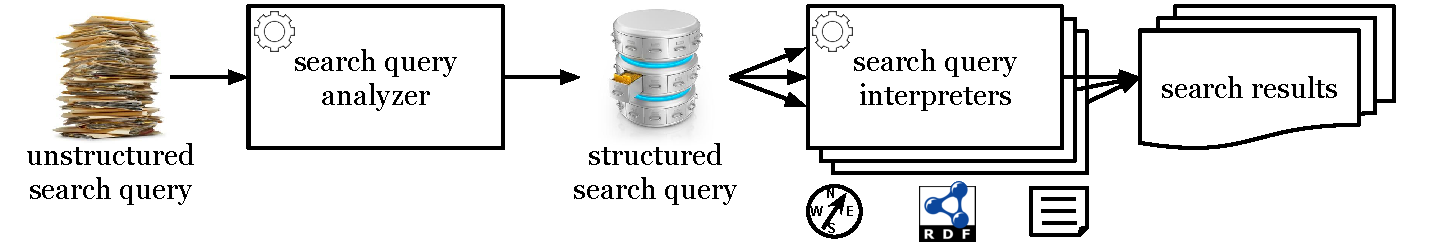
\includegraphics[width=\textwidth]{part_03/SEMANTiCS_architecture/highlevelarchitecture2}
\caption{High-level architecture of our distributed search framework.}
\label{fig:highlevelarchitecture}
\end{figure}


The concept of a service-oriented search framework poses several specific requirements that have to be met to rea\-lize a corresponding architecture.
They will be described in the following.
\todo[inline]{citation?}
\todo[inline]{or at least a note we came up with this ourselves? - CL\\will be at the last paragraph of the related work -- AnBo}
First of all, the framework has to ensure the integrability of the various intended search functionalities, which is derived from the properties of (extensible) service-oriented architectures:
%Derived from the properties of (extensible) service-oriented architectures, a generalized interface needs to enable the integration of various search functionalities.
%\todo[inline]{seems like a repetition to me}
%To ensure this, the following requirement has to be obeyed:
\begin{req}
An interface for search services has to be defined. The definition has to comprise a  summarization of all needed attributes for controlling the execution of (sub)queries.
\end{req}

We focus on a generalized approach, especially w.r.t. the communication across the diverse search services. Thus, we demand:
\begin{req}
The communication with the search services has to be stateless and transparent.
\end{req}
Derived from the required stateless and transparent communication, each search service has to encode all information about itself via its interface ,\ie in the message during the communication\footnote{This requirement is comparable to REStful communication~\cite{richardson2008restful} via the stateless HTTP protocol \url{http://tools.ietf.org/html/rfc7231}.}.
Hence, the information about each search service has be retrieved by querying the implemented interface methods.
%\todo[inline]{I don't get the last two sentences, to which requirement they belong and what they have to do with the next sentences? -CL\\Better? -- AnBo}
However, to provide a structured search query, an analysis of the textual user input is needed, which we consider to be beyond the scope of this paper. 
We will assume the search query is already available in a structured representation (\eg by having used approaches like~\cite{similarity,aqualog,tbsl}).
%For the sake of the limited space, we assume each search query to be already analyzed.
%That is, it was transformed into a structured representation, e.g., by using approaches like~\cite{similarity,aqualog,tbsl}.

\begin{req}\label{req:allrelevantparts}
The search query requires a structured representation which encapsulates information about all relevant parts of the search query. 
\end{req}

Hence, the high-level infrastructure of a federated search requires a two-step process:
\begin{enumerate}
\item search query analyzer
    \begin{itemize}
    \item input: unstructured search query
    \item output: structured search query
    \end{itemize}
\item search query interpreter
    \begin{itemize}
    \item input: structured search query
    \item output: ranked search results 
    \end{itemize}
\end{enumerate}
\todo[inline]{maybe markup structured search query everywhere\\ Why? -- AnBo}
\todo[inline]{Add reference to basic SOA paper at $\ast$ to support the seemingly arbitrary statement. --Max}
A graphical overview of the workflow is shown in Figure~\ref{fig:highlevelarchitecture}. 
To achieve the intended service-oriented architecture, it is crucial to hide the implementation details of the contained search services \cite{erl2008soa}.
As sketched in Figure~\ref{fig:highlevelarchitecture}, the structured search query is the main carrier of information.
Hence, no knowledge about the behavior of a particular search service may be contained in a structured search query, except in the case that it was computed by a search service itself. 
This is because the structured search query has to be independent from the particular implementation of any search service to ensure their exchangeability within the service-oriented architecture.
The following requirement is derived:
\begin{req}\label{req:independence}
The structured search query representation has to be independent from the implementation of any particular search service.
\end{req}

In the following, we will describe the data structure required for the representation of an analyzed search query.


\section{Search Query Representation}\label{chafedsearch:sec:searchqueryanalysis}

Understanding what the user is looking for is the starting point of every information retrieval process.
Yet, in the following section, the focus is not on the analysis of unstructured search queries.
Rather, search query analysis is considered a black box, \ie we focus on the representation of the structured search query after analysis.

%\subsection{Search Query Representation}
%Our representation is close to RDF.
%Hence, the following definition holds:
For our purpose, we build on a search query representation that is close to RDF:
\begin{definition}[RDF triples]
Assume there are pairwise disjoint infinite sets $I$, $B$, and $L$ representing IRIs\footnote{\textit{Internationalized Resource Identifier}, \ie a URI that may contain any Unicode character (cf.~\url{http://tools.ietf.org/html/rfc3987}).}, blank nodes, and RDF literals, respectively. 

A triple $(v_1, v_2, v_3) \in (I \cup B) \times I \times (I \cup B \cup L)$ is called an RDF triple. 
We call $v_1$ the subject, $v_2$ the predicate and $v_3$ the object. 
We denote the union $I \cup B \cup L$ by $T$ called RDF terms.
\end{definition}

However, we need a definition of the target resource.
Therefore, we allow a specific IRI to indicate the target elements, \ie our system performs a pure resource search.
For the sake of simplicity, we denote it as follows:


\todo[inline]{Warum sind es auf einmal urns? --RU}
\begin{definition}[Searched resource]
The place hold\-er for the searched resource is denoted as \placeholder.  
\end{definition}

\todo[inline]{Add example to clarify that \placeholder\ is what we actually search for and thus also acts as the root of the topologically sorted tree mentioned later. --Max}

Obviously, this mechanism can be used for referencing different variables by adding any ID (\eg \placeholderB).

\todo[inline]{The example query does not contain XXX used in its explanation later. Neither does the example in figures 2 and 3 contain the feature family-friendly. -CL}
For example, it is possible to express an actual search query, \eg \texttt{family-friendly hotel in Leipzig} in the following way:
Potential target hotels (\code{urn:id:hotel}) are restricted to those being located in the city center of Leipzig (expressed using the relation \code{urn:rel:cityCenter}).
Furthermore, a target hotel has to be marked (\code{urn:rel:hasFeature}) as family-friendly (\code{urn:id:familyFriendly}) and the description of the hotel has to contain the word \searchword.
The corresponding search query representation is shown in Figure~\ref{fig:ex1}.
\begin{figure}
\begin{center}
\begin{tabular}{llll}
$t_1$ & \placeholder & \code{owl:typeof} & \code{urn:id:hotel} \\
$t_2$ & \placeholder & \code{urn:rel:citycenter} & \code{urn:id:Leipzig} \\
$t_3$ & \placeholder & \code{urn:rel:description} & \placeholderB \\
$t_4$ & \placeholderB & \code{urn:rel:sublabel} & ``\searchword''
\end{tabular}
\end{center}
\caption{Example of a structured search query \texttt{family-friendly hotel in Leipzig} according to our RDF-like representation.}
\label{fig:ex1}
\end{figure}
\newcommand{\sstriplestore}{\code{urn:service:triplestore}}
\newcommand{\ssfulltext}{\code{urn:service:fulltext}}
\newcommand{\ssgeo}{\code{urn:service:gis}}
\begin{figure}[t]
\begin{center}
\begin{tabular}{lllll}
$t_1$ & \placeholder & \code{owl:typeof} & \code{urn:id:hotel} & ({\sstriplestore},250,500) \\
$t_2$ & \placeholder & \code{urn:rel:citycenter} & \code{urn:id:Leipzig} & (\ssgeo,100,400) \\
$t_3$ & \placeholder & \code{urn:rel:description} & \placeholderB & ({\sstriplestore},4000,1000) \\
$t_3$ & \placeholder & \code{urn:rel:description} & \placeholderB & (\ssfulltext,300,200) \\
$t_4$ & \placeholderB & \code{urn:rel:sublabel} & ``\searchword'' & (\ssfulltext,300,200) 
\end{tabular}
\end{center}
	\caption{Example of an annotated search query \texttt{family-friendly hotel in Leipzig}.}
	\label{fig:ex2}
\end{figure}



\subsection{Search Query Tagging}
Given the intention of using different search queries within a federated search architecture connecting diverse search functionalities, there is a need for separating a given search query into smaller parts.
These parts should be solvable by one or more search services providing the best match to the required search functionality.

In accordance with Requirement \ref{req:independence}, it is not allowed to encode the control of the execution directly within the representation of a (sub-)query.
Instead, the triples (\ie sub-queries) contained in the structured search query are assigned to \emph{every}\ search service for annotation.
That is, a sub-query is annotated with (a)~whether the given service is eligible for interpreting the sub-query, (b)~the estimated costs for processing the sub-query and (c)~the estimated number of results. 
%Instead, we chose to assign each search services each triple to tag of the search query.
%\todo[inline]{tag with what?}
%Thus, the query is sent to each search service concurrently. 
In particular, it is possible that a triple is tagged by several search services.
The annotation processes for a given sub-query are started for each search service concurrently.

After this step, the triples contained in a structured search query are annotated. 
Thus, the structured search query is now defined as follows:
\begin{definition}%[Structured Search Query with Annotations]
A set $A$ of pairs $(t,a)$ where $t$ is a triple of a search query $Q$ and $a$ is the annotation of a search service, is called structured search query with annotations. 
\end{definition} 
Note: It is possible that not all triples of $Q$ are annotated within $A$.
However, without loss of generality, it is assumed that all triples are tagged at least once.

To ensure performant computation of a query plan, an annotation is defined as follows:
\begin{definition}
A query annotation $a$ is a triple $(i,r,e)$, where $i$ is the IRI of the service, $r$ is the estimated number of results and $e$ is the estimated execution time (in milliseconds).
\end{definition}


\begin{figure}[p!]
\lstset{language=Java}
\begin{lstlisting}[frame=single]
/* compute topological order of the triples of the structured search query 
 * S P O is interpreted as directed edge S -> O with label P 
 * S,O are interpreted as nodes */
A scheduleSubQueries(A){
  List<node> resultList  // list will contain the ordered results
  Set<node> startSet= findNodesWithoutIncEdges(A) // set with nodes without incoming edges
  int orderTag = 0;
  while(!startSet.isEmpty()){
      n = startSet.pop() // removes a node 
      n.orderTag = orderTag++; // assign schedule order
      L.queue(n) // adds the node to the end of the list L
      for(node m where (n,m) in A){
          remove (n,m) from A
          if( no p exists with (p, m)){ // no other incoming edges for m
              startSet.push(m) 
          }
      }
  }
  if(hasEdges(A))
      return error // graph has at least one cycle
  else 
      return L // a topologically sorted order
}
\end{lstlisting}
\caption{Exemplary scheduler implementation}
\label{fig:scheduler}
\end{figure}

\begin{figure}[p!tb]
\centering
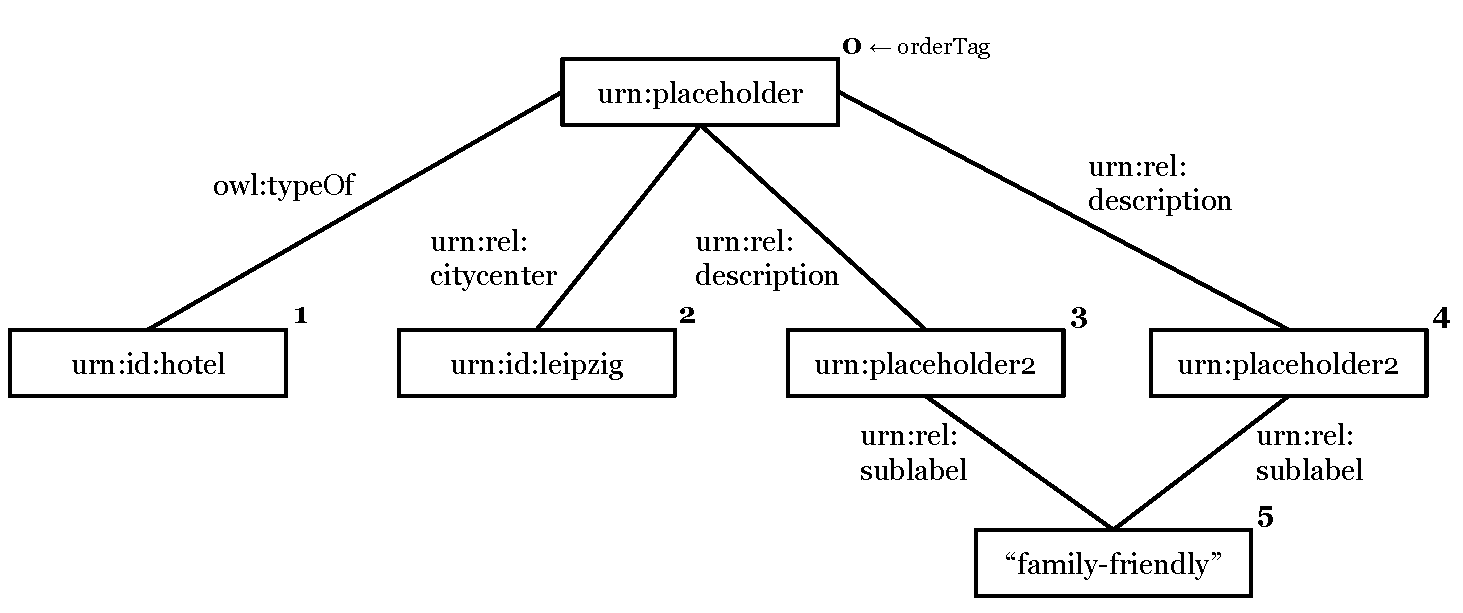
\includegraphics[width=\textwidth]{part_03/SEMANTiCS_architecture/query_plan_tree.pdf}
\caption{Scheduled query plan after topological sorting.}
\label{queryplantree}
\end{figure}



This definition satisfies Requirement \ref{req:allrelevantparts}.
Imagine a user wants to pose the following query to our framework: 
\begin{ex}
family-friendly hotel in Leipzig
\end{ex}

The annotated example query is shown in Figure~\ref{fig:ex2}.
In this example, \ssfulltext\ is an IRI of a service providing a full text search, \sstriplestore\ references a triple store and \ssgeo\ points to a search service encapsulating a GIS server.


\section{Search Query Interpretation}\label{chafedsearch:sec:queryinterpretation}

\todo[inline]{I don't get the following section at all! From the requirement that a query has to be interpreted by at least one service, how can we conlcude (``hence'') that the query plan is a topologically ordered graph with the result as root node? Maybe provide an example for clarity!? --Max}

Given a structured and annotated search query, a rea\-so\-nable query plan for the eligible search services has to be computed.
This can be done by scheduling algorithms with different optimization strategies. 
In this paper, we will focus on the general requirements only.

\todo[inline]{There is only one requirement, isn't there? So why focus on the ``general requirement\textbf{s}''? --Max}

\begin{req}
All triples of a structured and annotated search query have to be interpreted by at least one search service.
\end{req}
Note: As mentioned before, it is explicitly possible to have a triple interpreted by more than one search service.

Hence, a query plan can be computed by creating a to\-po\-lo\-gi\-cal order \cite{DBLP:books/aw/Knuth81}\ of the graph defined by the triples (\ie the triple S\,P\,O is interpreted as $S \xrightarrow{P} O$) of the structured search query where the result node is the root node of the graph.
A straight-forward implementation is shown in Fi\-gure \ref{fig:scheduler}.
There is numerous existing work dedicated to scheduler implementations \cite{XXX,YYY,ZZZ}.
A schedule graph is shown in Figure \ref{queryplantree} with respect to our running example.
\todo[inline]{Wo soll das Bild hin? Beschreibung?}


\section{Federated Search Architecture}\label{chafedsearch:sec:federated}

In this section, we present our federated search in\-fra\-struc\-ture. 
Particularly, it contains a service layer to which the diverse search services can be connected. 

\subsection{Search Service Interface}
For integration into the overall system, all search services have to implement a specific interface that facilitates exchangeability.
As a consequence, by implementing this given interface, services can be loosely coupled to the service layer.
The search service interface is defined as follows:
%\begin{figure}[h!tb]
\begin{lstlisting}[language=Java]
interface SearchService {
    /* annotation
     * in: search query Q
     * out: annotated search query A
     */ 
    A annotateQuery(Q);
    
    /* query execution 
     * in: annotated search query A
     * out: search results R
     */
    R executeQuery(A);
}
\end{lstlisting}
%\end{figure}
It is common to call \code{annotateQuery}\ with a complete structured query \code{Q}\ to get a complete annotated query \code{A}\ of all triples contained in \code{Q}.
Yet, the \code{executeQuery}\ method of an implementing search service is usually called passing only the sub-query the service is eligible for (\eg passing only the property \texttt{in Leipzig} to the geospatial search service).
Eligibility of a service is decided by the scheduler.

\subsection{Search Provider}
%The search provider provides an interface for search services that have implemented the search service interface.
%The definition of its interface is straight forward.
The search provider is an interface for integrated search services and defined as follows:
%\begin{figure}[h!tb]
\begin{lstlisting}[language=Java]
interface SearchProvider {
    /* query execution 
     * in: search query Q
     * out: search results R
     */
    R executeQuery(Q);
    
    /* search service registration 
     * in: IRI of the search service
     */
    void register(IRI);
    
    /* deregister a search service  
     * in: IRI of the search service
     */
    void deregister(IRI);
}
\end{lstlisting}
%\end{figure}
Hence, the search provider provides a method (\code{executeQuery}) for been accessed from a client while it also works as directory server (similar to a UDDI server \cite{UDDI}).
The directory functionality is achieved by the \code{register}\ and \code{deregister}\ methods allowing search services to connect and disconnect from the search provider.


%\subsection{Properties of the Architecture}
%The presented architecture separates different search functionality. 
%It decouples the search services from each other and  and allows an independent development, maintaince and 


% \subsection{Cache Layer}





\section{Conclusions}\label{chafedsearch:sec:conclusion}

We presented an architecture for a distributed search following the principles of service-oriented architectures. 
For this, we introduced a descriptive data representation, \ie the data representation does not contain implementation details of the underlying search services. 
Our implementation of such a structured search query is based on RDF.
After the tagging process, the annotated structured search query can be expressed using our RDF-like representation only.%, although, such a RDF representation will be very voluminous.
%However, we consider this as implementation detail. 

Our main contribution is the proposed architecture's capability of integrating and disintegrating (RDF unaware) search services dynamically.
This property is achieved by the descriptive message format as well as the ge\-ne\-ra\-lized service interface, which allows for a stateless and transparent communication with the integrated search services.
Hence, completely novel use cases are possible, in which search service integration happens on-the-fly to facilitate more dynamic environments.
Since the architecture is agnostic to the functionality of the search services, it is possible to integrate search services having not only (RDF-driven) semantic search functionalities but also other specialized search capabilities. 
For example, search services could comprise any specialized search functionality like ElasticSearch (providing high-performance federated large-scale full text search), or Web APIs encapsulating search functions with special semantics like SoundCloud\footnote{https://developers.soundcloud.com/}\ or Github\footnote{https://developer.github.com/}.
Our approach is superior as it does not burden these search services with the interpretation of the complete RDF (or SPARQL) standard.
Moreover, the architecture is scalable by design in the sense of the capability of integrating scalable and distributable search services. 
Finally, our \code{SearchProvider}\ provides a generalized interface being capable of receiving search queries via SPARQL (or any other representation, such as SQL or SeRQL). 
Therefore, a consolidated view on the dynamically summarized search services can be provided.
This allows for a transparent integration as a SPARQL endpoint, or using any other data access standard.

In the future, we will evaluate the capabilities of our architecture of providing rapid access to distributed data resources by comparing an implementation of the architecture to monolithic approaches. 
As possible data resources we consider datasets of the Linked Open Data Cloud as well as unstructured data provided by the Document Web in general or private data sets with restricted accessibility (by account or on the network level).
Hence, providing per\-so\-na\-lized search functionalities seems to be achievable.

Finally, the implementations are yet to be evaluated regarding performance and (re-)ranking issues. 
In the context of providing a distributed search, these are the main challenges considering the user's demands w.r.t.\ usability.

% However, increasing implementation details can lead to reducing the extendability with respect to search services which are not native to SPARQL.

%---

%Crucial for architecture -> rapid annotation has to be possible

%Requirements of the search queries w.r.t. SOA

%Evaluate the query plans with overlapping triple evaluation.

%Future:
%- sublabel
%- tighter integration
%- independent from the database of the search services 



%\bibliographystyle{abbrv}
%\bibliography{sigproc,refs} 
%\end{document}
%\documentclass{acm_proc_article-sp}
%\usepackage{times}
%\usepackage{microtype}
%\usepackage{url}
%\usepackage{graphics}
%\usepackage{graphicx}
%\usepackage{listings}
%\usepackage{wrapfig}

%\usepackage[utf8]{inputenc}
\lstset{basicstyle=\scriptsize \ttfamily, 
numbers=left, numberstyle=\tiny, stepnumber=1, numbersep=5pt}

%\usepackage{caption}
%\DeclareCaptionType{copyrightbox}
%\usepackage{subcaption}

%\usepackage{color}
%\usepackage[pdftex]{hyperref}
%\usepackage[]{algorithm2e}
%\usepackage{todonotes}
%\usepackage[disable]{todonotes}%


%\hypersetup{%
%pdftitle={Towards an Open Question Answering Architecture},
%pdfauthor={Marx Edgard and Usbeck Ricardo and  Ngomo Ngonga Axel-Cyrille and  H\"offner Konrad and Lehmann Jens and Auer S\"oren},
%pdfkeywords={Question Answering},
%bookmarksnumbered,
%pdfstartview={FitH},
%colorlinks,
%citecolor=black,
%filecolor=black,
%linkcolor=black,
%urlcolor=black,
%breaklinks=true,
%}
%\newcommand{\comment}[1]{}
\definecolor{Orange}{rgb}{1,0.5,0}
%\newtheorem{definition}{Definition}
%\newcommand{\urlfn}[1]{\footnote{\scriptsize\url{#1}}}

%\usepackage{enumitem}
%\setitemize{noitemsep,topsep=-6pt,parsep=0pt,partopsep=0pt}

%\pagenumbering{arabic}  % Arabic page numbers for submission.  Remove this line to eliminate page numbers for the camera ready copy
%\usepackage{cleveref}


%\widowpenalty = 10000
%\clubpenalty = 10000
%\begin{document}
%\crefname{section}{Section}{Sections}
%\crefname{figure}{Figure}{Figures}
%\crefname{table}{Table}{Tables}
% To make various LaTeX processors do the right thing with page size.
%\special{papersize=8.5in,11in}
%\setlength{\paperheight}{11in}
%\setlength{\paperwidth}{8.5in}
%\setlength{\pdfpageheight}{\paperheight}
%\setlength{\pdfpagewidth}{\paperwidth}
%\inputencoding{utf8}
% Use this command to override the default ACM copyright statement
% (e.g. for preprints). Remove for camera ready copy.
% \toappear{Submitted for review to WebSci 2012.}
% Ricardo Usbeck, Axel-Cyrille Ngonga Ngomo, Konrad H\"offner

\chapter{Towards an Open Question Answering Architecture}
%\title{Towards Open Interoperable Question Answering Modules} % Jens: just a title suggestion
%\numberofauthors{3}
%\author{
%  \alignauthor Edgard Marx\\
%    \affaddr{AKSW/BIS, Universit\"at Leipzig}\\
%    \affaddr{PO Box 100920, 04109 Leipzig, Germany}\\
%    \email{marx@informatik.uni-leipzig.de}%
%	\alignauthor Ricardo Usbeck\\
%       \affaddr{Universit\"at Leipzig, IFI/AKSW}\\
%       \affaddr{Unister GmbH, Leipzig}\\
%       \email{usbeck@informatik.\\uni-leipzig.de}%
%	\alignauthor Axel-Cyrille Ngonga Ngomo\\
%    \affaddr{AKSW/BIS, Universit\"at Leipzig}\\
%    \affaddr{PO Box 100920, 04109 Leipzig, Germany}\\
%    \email{ngomo@informatik.uni-leipzig.de}%
%	\and
%	\alignauthor Konrad H\"offner\\
%    \affaddr{AKSW/BIS, Universit\"at Leipzig}\\
%    \affaddr{PO Box 100920, 04109 Leipzig, Germany}\\
%    \email{hoffner@informatik.uni-leipzig.de}
%  \and%
%	\alignauthor Jens Lehmann\\
%    \affaddr{AKSW/BIS, Universit\"at Leipzig}\\
%    \affaddr{PO Box 100920, 04109 Leipzig, Germany}\\
%    \email{lehmann@informatik.uni-leipzig.de} \and 
%  \alignauthor S\"oren Auer\\
%    \affaddr{CS/EIS, Universit\"at Bonn}\\
%    \affaddr{R\"omerstra\ss e 164, 53117 Bonn, Germany}\\
%    \email{auer@cs.uni-bonn.de} 
%}

%\maketitle

%\begin{abstract} 
Billions of facts pertaining to a multitude of domains are now available on the Web as RDF data.
However, accessing this data is still a difficult endeavour for non-expert users.
In order to meliorate the access to this data, approaches imposing minimal hurdles to their users are required.
Although many question answering systems over Linked Data have being proposed, retrieving the desired data is still significantly challenging.
% no significant results were being achieved in last years.
In addition, developing and evaluating question answering systems remains a very complex task.
To overcome these obstacles, we present a modular and extensible open-source question answering framework.
We demonstrate how the framework can be used by integrating two state-of-the-art question answering systems.
As a result our evaluation shows that overall better results can be achieved by the use of combination rather than individual stand-alone versions.
%\end{abstract}

\section{Introduction}
\label{chaopenqa:sec:introduction}

Since its inception, the Web has been used by millions of users with the aim of sharing, reproducing and linking information.
More and more structured data, e.g.,~using the Resource Description Framework (RDF), is made available by users, services and more recently sensors.
Consequently, machines are now empowered to use a large amount of data available on the Web.
Examples of such datasets are \emph{DBpedia}~\cite{dbpedia-swj}\footnote{\url{http://dbpedia.org}, version 3.9} and \emph{LinkedGeoData}~\cite{SLHA11}\footnote{\url{http://linkedgeodata.org}, version of March 23rd, 2014}, which encompass more than 1 billion triples each.
The main advantage of these datasets is that they represent a variety of knowledge across several domains.
For example, \textit{astronauts who took part in the Apollo 14 mission} can be easily retrieved from DBpedia.
Although this data is accessible, users still face difficulties when trying to retrieve the desired information using traditional methods.

In particular, state-of-the-art search engines fail to retrieve the set of resources intended by the user because most of them abide by the \textit{bag of words} paradigm.
% instead of the question answering (QA) approach to dealing with user needs.
%This is the case of RDF data search engines.
For instance, the query \textit{Apollo 14 astronauts} on search engines such as Sigma\footnote{\url{http://sig.ma}} and Sindice\footnote{\url{http://sindice.com}} will retrieve relevant documents rather than the desired set of resources.
Furthermore, in some engines fail finding a suitable answer, due to no full understanding of the input query or not properly indexed data in the underlying knowledge base.

Over the last years, several approaches for question answering (QA) based on the Web of Data have been proposed. 
However, retrieving the desired data is still significantly challenging.
Reported results from the Question Answering on Linked Data (QALD) benchmark\footnote{\url{http://greententacle.techfak.uni-bielefeld.de/~cunger/qald}} indicate that  only $\approx54\%$ of the given questions were correctly answered in QALD-1 and $32\%$ in the more difficult QALD-2 and QALD-3 benchmarks.

In this paper, we present \emph{openQA}, an open source question answering framework that combines several question answering systems.
The proposed framework can facilitate the evaluation by promoting the modularization and easy integration of new modules via a plug-in architecture. 
Moreover, our experiments reveal a considerable improvement of correct answers by combining question answering systems, i.e., $87.5\%$ using the QALD-3 benchmark.

The remainder of this paper is structured as follows.
Section~\ref{chaopenqa:sec:rel} presents an background overview and related work.
Section~\ref{chaopenqa:sec:design} introduces the framework architecture and its components.
Section~\ref{chaopenqa:sec:impl} details the implemented components and used technologies.
Section~\ref{chaopenqa:sec:eval} presents the achieved results.
Finally, Section~ref{chaopenqa:sec:conc} concludes with an outlook on future work.
\\\\
\section{Background and Related Work}\label{chaopenqa:sec:rel}

The World Wide Web Consortium recommend the use of Linked Data (LD) standard to represent and publish open data\footnote{\url{http://www.w3.org/standards/semanticweb}}.
The LD standard uses for the representation of data (facts, rules and their relationships) the \emph{RDF} format.
%This can formally be defined as follows:
%\vspace{-4.0mm}
%\begin{definition}[RDF definition]
%\label{def:triple}
%Let \emph{I}, \emph{B} and \emph{L} be an infinite disjoint sets of IRIs, Blank Nodes and RDF literals respectively.
%We set \textit{RDF terms} as being an infinite set of $m \in T$ where $T:=I \cup B \cup L$.
%Being the subject, predicate and object sets respectively defined by $S:={I \cup B}$, $P:={I}$ and $O:={I \cup B \cup L}$.
%A triple $t:=(m_s, m_p, m_o)$ is called an RDF \textit{triple} iff $m_s \in S$, $m_p \in P$, and $m_o \in O$.
%\end{definition}
%\begin{definition}[RDF Instance]
%\label{def:instance}
%A set of $n$ triples $E:=\{$ $t_0,$ $t_1,$ $t_2...t_n$ $\}$ is called RDF \textit{instance} $\Leftrightarrow \exists !$ $v_s \in S$ and $n \geq 1$.
%\end{definition}
%\begin{definition}[Knowledge base]
%\label{def:knowledgebase}
%The knowledge base $L$ is an union of a set of triples describing a set of classes $C$ and their instances $E$.
%$L \subset T : L:= C \cup E$
%\end{definition}
%\todo{Ricardo: classes and instances is not defined}

Question answering on linked data is an active and diverse research field with many existing research prototypes designed for different environments.
Systems running on a \emph{closed domain} are optimized for and only work on a specific knowledge base or field, like biology~\cite{biomedicalqa} or medicine~\cite{medicalqa}.
Since they do not need to integrate different schemas and knowledge bases and thus suffer less from ambiguity, they generally create faster and higher-quality results.
%Reuse and portability is however severely restricted.
However, closed-domain approaches lack flexibility.
Additionally, there are high costs when adapting such a system to a new domain or implementing a new system.
Thus, the research focus has been moved towards multi-purpose, open-domain QA systems like FREyA~\cite{freya} or hybrid approaches like TBSL~\cite{unger2012template} with a domain unspecific core and a domain specific, adaptable extension.

Question answering is a complex process which consists of many different steps, most of which have to be executed in a sequential manner and are thus called a pipeline.
Some of those steps, like natural language processing (NLP), which involves parsing and part-of-speech extraction can make use of mature, well performing tools.
No such simple solution exists however for the step of interpretation -- the process of extracting the meaning of a question.
%However, although the process of interpretation is very important on question answering systems, they do not rely on that.

%In the follows subsections we group the related work into two categories: (1) answer formulation and (2) presentation.
%Answer formulation (1) encompasses approaches for generating answers over natural language (NL) input queries whereas presentation, for better displaying the formulated answer.

%\subsection{Answer formulation}
FREyA~\cite{freya} is different from SPARQL driven systems and makes use of a combination of syntactic parse trees, phrases potentially representing ontologies as well as ontology concepts.
Phrases potentially representing ontology concepts, so-called \emph{Potential Ontology Concepts (POCs)} are identified by heuristics on the syntactic parse tree.
\emph{Ontology Concepts (OCs)}, are resources from an ontology that are identified matching their labels with phrases from the question without regarding its structure.
A consolidation algorithm then matches POCs to OCs.
In case of ambiguities, feedback from the user is asked.
Disambiguation candidates are created using string similarity in combination with WordNet synonym detection.
The system learns from the user selections, thereby improving the precision over time.
However, user feedback is rare and expensive.

Most frequently, QALD systems uses a set of predefined graph pattern templates in the interpretation process to generate SPARQL queries representing the input question.
The use of SPARQL queries enables the representation of a more complex semantic structure of the original natural language question,
going beyond the limitation of triple-only-based systems.
However, the strategy used to generate the graph patterns and consequently the SPARQL query differs significantly between approaches.
This is the case of \emph{SINA}~\cite{SHE+13}, \emph{TBSL}~\cite{unger2012template} and \emph{Casia}~\cite{clef2013casia}.

\emph{SINA} is a question answering system that uses the knowledge base itself to formulate the graph pattern templates.
The system deals with the input query as being a set of keywords, which enable the interpretation of keyword as well as full question fashion queries.
In order to prune the number of generated graph pattern templates, \emph{SINA} uses a statistical Hidden Markov model.

\emph{TBSL} is another template-based question answering system for LD.
Different from other approaches, \emph{TBSL} uses an entity identification and predicate detection method to fill the slots of the previosuly defined SPARQL template query with data extracted from the original query.

\emph{Casia}~\cite{clef2013casia} generates the graph pattern templates by using the question type, named entities and POS tags techniques.
The generated graph patterns are then mapped to resources using Wordnet, PATTY and similarity measures.
Finally, the possible graph pattern combinations are used to build SPARQL queries.

As each of these systems has its strengths and weaknesses, we move a step further, adopting a composed solution.

\section{Framework Design}
\label{chaopenqa:sec:design}

\begin{figure*}[bht]
	\centering
	\includegraphics[width=.97\textwidth]{part_03/SEMANTiCS_openQA/images/architecture.pdf}
	\caption{openQA Architecture Overview.}
	\label{chaopenqa:fig:architecture}
	\vspace{-4.0mm}
\end{figure*}
We propose a framework for combining different approaches to question answering.
The design was made taking into account the architecture of classic and over linked data QA systems, search engines, smart assistants as well as hybrid systems such as IBM Watson \footnote{\url{http://www.ibm.com/smarterplanet/us/en/ibmwatson}}.
In the following, we explain our \emph{openQA} framework architecture which consists of four main modules comprising several sub modules, see Section~\ref{chaopenqa:fig:architecture}.
The framework has a main work-flow comprising four stages (\emph{interpretation}, \emph{retrieval}, \emph{synthesis},  %and %\emph{resolution}, 
\emph{renderization}) and adjacent modules (\emph{context} and \emph{service}).
The adjacent modules are intended to be accessed by any of the components of the main work-flow.

One of the biggest challenges in realizing a generic framework is how to combine different approaches.
To tackle this challenge, the framework was designed in a plug-in architecture style.
Plug-in architectures are known for promoting modularization and easy integration.
We aim that the openQA architecture allows to support the diversity of many existing Linked Data question answering systems. % and is organized as follows.
\emph{openQA} is organized as follows:
\vspace{-4.0mm}
\paragraph{\textbf{Answer Formulation}} The core module comprises the \emph{answer formulation} process, its purpose is to receive an input query and deliver the most probable answer candidates.
The answer formulation process is composed by four different stages:
\vspace{-3.0mm}
\begin{enumerate}
	\item \emph{Interpretation} The first and crucial step of the core module is the \emph{interpretation}. 
	Here, the framework attempts to generate a formal representation of the (intention behind the) input question.
	By these means, it also determines how the input question will be processed by the rest of the system.	
	Because the interpretation process is not trivial, there is a wide variety of techniques that can be applied at this stage, such as tokenization, disambiguation, internationalization, logical forms, semantic role labels, question reformulation, coreference resolution, relation extraction and named entity recognition amongst others.
	Most of these technologies are well understood and will not be discussed here.
	The interpretation stage can generate one or more interpretations of the same input in different formats such as SPARQL, SQL or string tokens.
	\item \emph{Retrieval} After an interpretation of the given question is generated, the \emph{retrieval} stage extracts answers from sources according to the delivered interpretation format or content.
	For instance, one of the outputs of the interpretation can be: 
	(1) a SPARQL query which can be handled by a triple store;
	(2) an SQL query which will be processed by a relational database, or;
	(3) a set of keywords that can be sent to a document-based search engine.
	Specific interpretations can also be used for extracting answers from sources such as web services.		
	\item \emph{Synthesis} %After a set of answer candidates be founded by the retrieval stage, a synthesize stage is required.
	Answers may be extracted from different sources, be ambiguous and redundant.
	To alleviate this issues the \emph{Synthesis} stage processes all information from different retrieval sub-modules.
	Results that appear multiple times are fused with an occurrence attribute that helps to rank, cluster and estimate the confidence of the retrieved answer candidates.
	The \emph{Synthesis} process is closed by \textit{Section \ref{def:synthesis}}.

\end{enumerate}
\vspace{-5mm}
\begin{definition}[Synthesis]
\vspace{-2.0mm}
\label{def:synthesis}
Let $R_1, \ldots, R_n$ be the result sets generated by different search. 
The result of the synthesis process is a duplicate-free result set $R=\bigcup\limits_{i=1 \ldots n} R_i$. % such that $\forall x \in R$ and $y \in R$ we will have $x = y$. 
The ranking of the results in $R$ is left open to the user but must be specified by the means of an injective function $pos$ which maps each $r \in R$ to exactly one value between 1 and $|R|$.
 
%Considering a series of answer candidates $R$ of type $w$, $R:=\{w_0,w_1,w_0,$ $w_2...w_n\}$, composed by a series of \textit{RDF Terms} of type $t \in T$ retrieved from one or more SPARQL queries.
%The synthesis process is covered by the function $synthesis(R)=R'$, where the position of $w' \in R'$ is given by the function $pos(w')$ and the following holds:
%\[\forall w \in R, \exists! w' \in R', w=w'\]
\vspace{-5.0mm}
\end{definition}

%The retrieved answer candidates can be from different explored graphs and formats: video, image, document and resource.	
%The syntheses stage is also designed for cluster all the related entity information.
%	\item \emph{Resolution} The last stage is the resolution.
%	The resolution stage can apply filters to remove noise, choose or re-arrange the most promising candidates.
%	The usage of machine learning is also encouraged.
%	Machine learning allows the system to better rank and select the synthesized candidates which allows the system to produce better results in future queries.
\vspace{-3.0mm}
\paragraph{\textbf{Renderization}}
Typically a knowledge base comprises data in several types and formats.
Each type of information demands a specific display style to deliver the best possible amount of information to the user.
In the proposed architecture the concepts of answer \emph{formulation} and \emph{presentation} are detached.
The \emph{renderization} module encapsulates the answer presentation and comprises one or more renders that work as widgets.
That is, each widget plugged to the \emph{renderization} module can be used to render one type or format of data.
\vspace{-4mm}

\paragraph{\textbf{Context}} Users context can help the answer personalization providing information such as who or where is the user, what is the preferred language or if the question is one of a series of related previous questions.
To enable the system to produce better answers the \emph{context} module can store users information, such as location, statistics and previous queries.
\vspace{-4mm}
\paragraph{\textbf{Services}} The \emph{services} modules are designed to be easily accessed by the components. 
They intend to facilitate the encapsulation, addition and sharing of application functionalities between the modules i.e.:% so it can be shared amongst them.
\vspace{-3.0mm}
\begin{enumerate}
	\item \emph{Cache} The result of a determined parameter in a function can be required multiple times. The \emph{cache} service intends to provide efficiency while prevents the execution of the same process multiple times.
	It stores the results of processes in order that future requests to the same process can be executed faster.
	\vspace{-2.0mm}
	\item \emph{Knowledge Summarization}
	Currently, the \emph{DBpedia}\footnote{\url{http://wiki.dbpedia.org/About}} dataset comprises millions of facts distributed over millions of entities, but not all this data is useful for users.
	\emph{Knowledge Summarization} has an important role in knowledge presentation.
	Knowledge summarization refers to a combination of two techniques, set and entity summarization.
	Set and entity summarization consist of the use of heuristics to rank respectively entities and their attributes.
	\vspace{-4.0mm}
\end{enumerate}

\begin{figure}
	\centering
	\includegraphics[width=\columnwidth]{part_03/SEMANTiCS_openQA/images/sample_page.pdf}	
	\caption{Screenshot of the demo available at \url{http://openqa.aksw.org}.}
	\label{chaopenqa:fig:demo}
	\vspace{-4.0mm}
\end{figure}

\section{Implementation}
\label{chaopenqa:sec:impl}

The framework is implemented as open-source and additionally provides several built-in components and information about: (1) possible log messages, (2) used memory, (3) errors as well as (4) answered and not answered queries.
Figure~\ref{chaopenqa:fig:architecture} gives an overview of the implemented modules in gray.
Moreover, a test integration framework was developed in order to run evaluation queries on \emph{openQA} and the underlying modules.

\paragraph{\textbf{Combining Approaches}}
\vspace{-4.0mm}
%The remaining of the framework is structured as follows.
Regarding \emph{Knowledge Summarization}, an algorithm based on \emph{Relin}~\cite{cheng2011relin} has been added.
\emph{SINA} and \emph{TBSL} were combined as interpretation modules.
The framework can handle SPARQL queries over a retrieval component based on the \emph{Jena}\footnote{\url{http://jena.apache.org}} client.
The synthesis module is inspired by~\cite{conf/aswc/LopezNFSUM09} and formalized by definition \ref{def:synthesis} in which $pos(r) = - \log(|r|/|R|)$, i.e., the more occurrences an answer has, the more confidence it provides.
The renderization module of \emph{openQA} uses \emph{Infograph}.
\emph{Infograph} is a render API developed for \emph{openQA} that can render (1) SPARQL queries, (2) literals and (3) entities from knowledge bases.
Infograph is capable of differentiating entities with and without geographic information as well as automatically generate entity descriptions based on their attributes via \emph{SPARQL2NL}~\cite{sparql2nl-demo}, in case the entity does not have a description.

\section{Evaluation}
\label{chaopenqa:sec:eval}

The evaluation of the described framework was performed measuring improvement of correct answered queries in QALD-3 by combining the participant systems.
Furthermore, the framework was assessed with the fourth version of the same benchmark (QALD-4), by using stand-alone versions of \emph{TBSL} and \emph{SINA} as well as a combination of both.
All evaluations were executed over the multilingual tasks.
The correctness and incorrectness synthesized answer from different systems is given by logical conjunction.
According to QALD benchmark the result from the synthesis operations should be equal to the given correct answer set $C$ otherwise is considered incorrect.
\[\forall x \ C(x) \iff \bigvee_{i=1}^n R_i(x)\]

\vspace{-4.0mm}
The QALD-3 evaluation (Figure~\ref{chaopenqa:fig:combining}) shows that a significant improvement of correct answers can be achieved (87.5\%) by using a theoretical combination of all the participant systems.

Regarding QALD-4, we measure a combination of the current implemented versions of \emph{SINA} and \emph{TBSL} (trained respectively using QALD-2 and QALD-1). 
As both systems were still under major revision, the tests were focused in how much improvement could be achieved under their combination. 
The results reveal that a combination of both systems is also better than a stand-alone versions, leading to an improvement of 11\% in correct answered queries.

\begin{figure}[h]
	\centering
	\includegraphics[width=\columnwidth]{part_03/SEMANTiCS_openQA/images/right_answers.pdf}	
	\caption{Correct answers on combining QALD-3 systems.}
	\label{chaopenqa:fig:combining}
\end{figure}

The framework (Figure~\ref{chaopenqa:fig:demo}) is available over two public instances,
one using \emph{SINA} (\url{http://sina.aksw.org}) and another using both, \emph{SINA} and \emph{TBSL} (\url{http://openqa.aksw.org}).
As the live instances rely on the public \emph{DBpedia} endpoint, the user's experience can be affected by instabilities.
Regarding this, a demo video is also available at \url{http://www.aksw.org/Projects/openQA}.

\vspace{8.0mm}
\section{Conclusions and Future Work}
\label{chaopenqa:sec:conc}

The proposed architecture is part of a larger research agenda which aims to define and develop a common framework for question answering systems.
%It is also a complement of work of set of specialists and technologies.
Therefore, we have implemented several components, which are open source and can be downloaded, plugged and extended \footnote{\url{http://aksw.org/Projects/openQA}}.
The achieved results indicate that the \emph{openQA} architecture can be used as a base for developing, combining and evaluating question answering systems.
The next efforts will consist of integrating unstructured sources, such as text extracted data from web pages and document bases.
Furthermore, we want to extend the implemented modules with non-commercial APIs from other question answering systems and evaluate them against several well-know benchmarks. 

%\vspace{-5mm}
%\bibliographystyle{abbrv}
%\bibliography{aksw,references}
%\end{document}

%\chapter{Autonomous QA}

\chapter[HAWK -- Hybrid Question Answering using Linked Data]{HAWK -- Hybrid Question Answering}
\graffito{
HAWK has been developed to bridge the gap between unstructured and structured knowledge bases in \ac{QA}. 
The approach is described by the corresponding publications~\cite{HAWK_CLEF_2015,HAWK_NLIWOD_2015,hawk_2015} mainly authored by the thesis author.
HAWK won the 2nd price at the \ac{QALD} challenge, task 2 2015.
}
\label{cha:hawk}
Recent advances in \ac{QA} over \ac{LD} provide end users with more and more sophisticated systems for querying \ac{LD} by allowing users to express their information need in natural language~\cite{SINA_WebSemantic,pythia,template}. 
This allows access to the wealth of semantic data available on the Semantic Web to non-experts and users unaware of the underlying schema. 
Linked Data simplifies the access to structured and semantic meaningful information more than unstructured Web documents can.
However, a lot of information is still available only in textual form, both on the Document Web and in the form of labels and abstracts in \ac{LD} sources~\cite{GER+13}.
Therefore, a considerable number of questions can only be answered by using hybrid question answering approaches, which  can find and combine information stored in both structured and textual data sources~\cite{combiningLDandIR}.

In this chapter, we present HAWK, the first full-fledged hybrid \ac{QA} framework\footnote{To the best of our knowledge.} for entity search over \ac{LD} and textual data. 
%To the best of our knowledge, this is the first hybrid question answering system, combining information from structured and unstructured data.
Given a textual input query $q$, HAWK implements a 13-step pipeline, which comprises 1) input segmentation 2) part-of-speech tagging, 3) detecting entities, 4) spotting noun phrases, 5) dependency parsing and 6) applying linguistic pruning heuristics for an in-depth analysis of the natural language input. 
The results of these first six steps is a predicate-argument graph annotated with resources from Linked Data. HAWK then 7) assigns semantic meaning to nodes and 8) generates basic triple patterns for each component of the input query with respect to a multitude of features. 
This deductive linking of triples results in a set of SPARQL queries containing text operators as well as triple patterns.
In order to reduce operational costs, 9) HAWK discards queries using several rules, e.g., by  discarding not connected query graphs.
10) HAWK uses a prefix-based classifier to decide whether it is boolean question and depending on the result 11) modifies the SPARQL query or 12) calculated the query modifiers.
Finally, 13) queries are ranked using extensible feature vectors and cosine similarity.
%%We evaluate HAWK on the \ac{QALD}-4 benchmark\footnote{\url{http://www.sc.cit-ec.uni-bielefeld.de/qald/}} for hybrid question answering. 
%As data source it uses a triple store containing DBpedia 3.9 as well as full-text information based on the Wikipedia abstracts of all loaded resources.
%The evaluation sections reports on micro F-measure, and analyzes the influence of different entity annotation systems on the overall question answering performance.
%\todo[inline]{@Axel: Contribs}
Our main contributions can be summarized as follows:
 \begin{itemize}
 \item We present the first \ac{QA} framework for answering hybrid questions;
 \item HAWK analyses input queries based on predicate-argument trees to deeply understand and match semantic resources;
 \item Our framework is generic, as it does not rely on templates. Thus, it is inherently able to cover a wide variety of natural language questions. % as well as knowledge bases with various topologies;
 \item The modular architecture of HAWK allows simple exchanging of pipeline parts to enhance testing and deployment;
 %\item HAWK's implementation is open-source under MIT License\footnote{\url{https://github.com/AKSW/hawk}};
 \item Our evaluation suggests that HAWK is able to achieve F-measures of 0.61 on a rather small (<50 questions) training datasets.
 \item We present a thorough evaluation of the framework, including an analysis of the influence of entity annotation frameworks on the generation process of the hybrid queries and a study of the overall accuracy of the system. 
 \item Furthermore, HAWK can generate SPARQL queries using \texttt{ASK}. Our results show that these developments lead to HAWK achieving 0.74 F-measure on the ASK queries contained in the Question Answering over Linked Data (\ac{QALD}-5) hybrid query benchmark~\cite{qald5} assuming an given optimal ranking function.
 \end{itemize}

The remaining chapter is structured as follows:
We explain HAWK's methodology in detail in Section~\ref{chahawk:sec:method} and illustrate the pipeline steps on several examples in Section~\ref{sec:hawkexample}.
HAWK's performance and the influence of entity annotation systems is evaluated in Section~\ref{chahawk:sec:evaluation}. 
%Section~\ref{chahawk:sec:relatedwork} discusses related work.  
%Finally, we conclude in Section~\ref{chahawk:sec:conclusion}. 
Additional information can be found at our project home page \url{http://aksw.org/Projects/HAWK.html}.

\section{Method}
\label{chahawk:sec:method}

In the following, we describe the architecture and methodology of HAWK. 
Figure~\ref{fig:hawk_pipeline} gives an overview of the architecture. %In the following we describe the depicted steps in more detail.%: POS-tagging, entity annotation, dependency parsing, linguistic pruning, semantic annotation, SPARQL query generation, pruning and ranking.

\begin{figure}[tb!]
\centering
\usetikzlibrary{positioning,shapes,arrows}
% Define block styles
\tikzstyle{decision} = [diamond, draw, fill=blue!20, 
    text width=5em, text badly centered, node distance=3cm, inner sep=0pt]
\tikzstyle{block} = [rectangle, draw, fill=blue!20, 
    text width=5.5em, text centered, rounded corners, minimum height=4em]
\tikzstyle{line} = [draw, -latex']
\tikzstyle{cloud} = [draw, ellipse,fill=red!20, node distance=3cm,
    minimum height=2em]

\begin{tikzpicture}[->,node distance = 3cm, auto]
    % Place nodes
    \node [cloud] (question) {Question};
    \node [block, right of=question] (segmentation) {Segmen\-tation};
    \node [block, right of=segmentation] (pos) {POS-Tagging};
    \node [block, right of=pos] (entityannotation) {Entity Annotation};
    \node [block, below of=entityannotation, node distance=2.2cm] (nounphrasedetection) {Noun Phrase Detection};
    \node [block, left of=nounphrasedetection] (dependency) {Dependency Parsing};
    \node [block, left of=dependency] (ling_heu) {Linguistic Heuristics};
    \node [block, left of=ling_heu] (sem_anno) {Semantic Annotation};
    \node [block, below of=sem_anno,node distance=2.2cm] (sparql) {Hybrid SPARQL generation};
    \node [block, right of=sparql] (sem_pruning) {Semantic Pruning};
    \node [decision, right of=sem_pruning] (classify) {ASK Classifier};
    \node [block, below left of=classify] (mod_ask) {Modify SPARQL Query};
    \node [block, below right of=classify] (calc_card) {Calculate Cardinality};
    \node [block, below of=classify,  node distance=4cm] (rank) {Rank queries};
    \node [block, left of=rank] (sparql_fire) {Hybrid SPARQL Store};
    \node [cloud, left of=sparql_fire] (answer) {Answer};
    %\node [decision, below of=evaluate] (decide) {is best candidate better?};
    % Draw edges
    \draw[->]  (question) -- (segmentation);
    \draw[->]  (segmentation) -- (pos);
    \draw[->]  (pos) -- (entityannotation);
    \draw[->]  (entityannotation) -- (nounphrasedetection);
    \draw[->]  (nounphrasedetection) -- (dependency);
    \draw[->]  (dependency) -- (ling_heu);
    \draw[->]  (ling_heu) -- (sem_anno);
    \draw[->]  (sem_anno) -- (sparql);
    \draw[->]  (sparql) -- (sem_pruning);
    \draw[->]  (sem_pruning) -- (classify);
    \draw[->]  (classify) -- (mod_ask);
    \draw[->]  (classify) -- (calc_card);
    \draw[->]  (mod_ask) -- (rank);
    \draw[->]  (calc_card) -- (rank);
    \draw[->]  (rank) -- (sparql_fire);
    \draw[->]  (sparql_fire) -- (answer);


   % \path [line] (decide) -| node [near start] {yes} (update);
   % \path [line] (update) |- (identify);
   %    \path [line] (decide) -- node {no}(stop);
\end{tikzpicture}
\caption{Architecture of HAWK.}
\label{fig:hawk_pipeline}
\end{figure}

\subsection{Input Segmentation.} 
To be generic with respect to the language of the input question, HAWK uses a modular system that is able of tokenizing even languages without clear separation like Chinese\footnote{\url{https://github.com/clir/clearnlp}}.
For English input questions our system relies on the \emph{clearNLP}-framework~\cite{choi2011getting} which provides a.o. a white space tokenizer, Part-of-Speech (POS)-tagger and transition-based dependency parsing.

\subsection{Part-of-Speech (POS)-Tagging.} 
HAWK annotates each token with its POS-tag, which will be later used to identify possible semantic annotations. 
A large number of frameworks have been developed for these purposes over the last years. 
Currently, we rely on \emph{clearNLP}~\cite{choi2011getting} which is a fast and robust framework~\cite{choi-palmer:2012:ACL2012short}.

%\subsection{POS-Tagging, Segmentation}
%\todo[inline]{re is no tokenisation/segmentation component in the pipeline?}
%A large number of frameworks have been developed for these purposes over the last years. 
%We rely on \emph{clearNLP}~\cite{choi2011getting} which is based on transition-based dependency parsing and sophisticated segmentation algorithm.

\subsection{Entity Annotation}
HAWK identifies named entities and tries to link them to semantic entities from the underlying knowledge base, in our case DBpedia 2014\footnote{Status of May 2015. The dataset choice is influenced by the benchmark requirements.}, via well-established entity annotation frameworks, also called entity tagging tools:
\begin{itemize}
\item \textbf{Wikipedia Miner}~\cite{milne2008learning} is based on different facts like prior probabilities, context relatedness and quality, which are then combined and tuned using a classifier.
\item \textbf{DBpedia Spotlight}~\cite{spotlight} %, one of the first semantic entity annotation approaches, 
was published in 2011. 
This system combines named entity recognition and disambiguation based on DBpedia.
\item \textbf{TagMe 2}~\cite{TagMe2} is based on a directory of links, pages and an inlink graph from Wikipedia.
The approach recognizes entities by matching terms with Wikipedia link texts and disambiguates the match using the in-link graph and the page dataset.
%Afterwards, TagMe 2 prunes identified named entities which are considered as non-coherent to the rest of the named entities in the input text.  
\item \textbf{FOX}~\cite{FOX} has been introduced 2014 as an ensemble learning-based approach combining several state-of-the-art named entity recognition approaches. 
The FOX framework outperforms the current state of the art entity recognizers and relies on the entity linking framework AGDISTIS~\cite{agdistis_iswc}.
\end{itemize}
Additionally, we implemented two artificial spotters for evaluation:
\begin{itemize}
\item \textbf{Union} is a spotter that combines the result sets of the above introduced spotters and returns thus a superset of all spotters.
\item \textbf{Optimal} will spot all entities from the gold standard to be able to ignore spotting influences in the following steps of the pipeline.
\end{itemize}

HAWK annotates the POS-tag \texttt{ADD} to these named entities to differentiate named entities from other tokens. % for our running example from above.
The influence of the entity annotation module is evaluated in Section~\ref{chahawk:sec:evaluation}.

\subsection{Noun Phrase Detection.}
HAWK identifies noun phrases, i.e., semantically meaningful word groups, e.g., real-world entities or concepts not captured by the underlying knowledge base or not yet recognized by the entity annotation system, using the result of the POS-tagging step. 
This step is also know as chunking. 
Input tokens are combined following manually-crafted linguistic heuristics based on POS-tag sequences derived from the \ac{QALD}-5 benchmark questions and their POS-tag is changed to \texttt{CNN} which we introduce to the system.
Two domain experts implemented the deduced POS-tag sequences and safeguarded the quality of this algorithm w.r.t. the \ac{QA} pipeline F-measure. 
The full process can be found in Algorithm~\ref{listing:nouncombiner}.

\begin{algorithm}[tb!]
\SetAlgoLined
\KwData{Tokenized question ($list$) with Part-of-Speech-tags (POS-tags)}
	subsequence = ()\;
	\For{$t \in [0,|list|]$ }{
			token = list.get($t$)\;
			%// look for start "RB|JJ|NN(.)*"
			\eIf{$subsequence = \emptyset$}{
			    \lIf{$pos(t) \in (\mathrm{CD|JJ|NN(.)^*|RB(.)^*})$} {
				subsequence.add(token)
				}
			}
			%// split "of the" or "of all" via pos\_i=IN and pos\_i+1=DT
			{
    			\uIf{$t + 1 < |list| \wedge pos(t) \in (\mathrm{IN}) \wedge pos(t+1) \in (\mathrm{(W)?DT})$} {
    				\lIf{$subsequence.size() >= 2$} {
    					combine(subsequence)
    				}
    		        subsequence = ()\;
    			}
    		%	// do not combine NNS and NNPS but combine "stage name", "British Prime minister"
    			\uElseIf{$pos(t - 1) \in (\mathrm{NNS}) \wedge pos(t) \in (\mathrm{NNP(S)?})$} {
    			    \lIf{$subsequence.size() > 2$} {
    					combine(subsequence)
    				}
    		        subsequence = ()\;
    			}
    		%	// finish via VB* or IN -> null or IN -> DT or WDT (now a that or which follows)
    			\uElseIf{$!pos(t - 1) \in (\mathrm{JJ|HYPH}) \wedge (pos(t) \in (\mathrm{VB|WDT|IN})))$} {
    		%		// more than one token, so summarizing makes sense
    			    \lIf{$subsequence.size() > 1$} {
    					combine(subsequence)
    				}
    		        subsequence = ()\;
    			}
    		    \uElseIf{$pos(t) \in (\mathrm{NN(.)^*|RB|CD|CC|JJ|DT|IN|PRP|HYPH|VBN})$} {
    				subsequence.add(token)
    			}
    			\uElse{
    		        subsequence = ()\;
    			}
    		}
        }
\caption{Algorithm for combining noun phrases.}
\label{listing:nouncombiner}
\end{algorithm}




\subsection{Dependency Parsing}

Subsequently, in order to capture linguistic and semantic relations, HAWK parses the query using dependency parsing~\cite{choi2011getting}.
The dependency parser is given the chunked question. 
The generated pre\-dicate-argument tree is directed, acyclic and all its nodes contain their POS-tags as well as their labels.
HAWK's modular structure allows for an easy exchange of the POS-tagger or dependency parser.

\subsection{Linguistic Pruning}

The natural language input can contain tokens that are meaningless for retrieving the target information or even introduce noise in the process.
HAWK therefore prunes nodes from the predicate-argument tree based on their POS-tags, e.g., deleting all \texttt{DET} nodes, interrogative phrases such as \texttt{Give me} or \texttt{List}, and auxiliary tokens such as \texttt{did}.
Algorithm~\ref{listing:lingpruning} details the process for removing nodes.

\begin{algorithm}[tb!]
\SetAlgoLined
\KwData{Dependency-argument tree with Part-of-Speech-tags}
Queue queue = [tree.getRoot()]\;
\While{$queue != \emptyset$} {
	node = queue.poll()\;
    \If{$pos(node) \in (\mathrm{WDT|POS|WP\$|PRP\$|RB|PRP|DT|IN|PDT})$} {
	tree.remove(node)\;
}
	queue.add(node.getChildren())\;
}
\If{$root.label == ("Give")$} {
	\For{$childNode \in root.getChildren()$} {
		\lIf{$childNode == "me"$} {
			tree.remove(childNode)
		}
	}
}
\lIf{root.label $\in\{ "List", "Give"\}$}{
	tree.remove(root)
}
\caption{Algorithm for pruning noisy nodes}
\label{listing:lingpruning}

\end{algorithm}



\subsection{Semantic Annotation}
After linguistic pruning, HAWK annotates each node in the tree with possible concepts from the knowledge base and its underlying ontology.
To this end, our framework uses information about possible verbalizations of ontology concepts based on both \texttt{rdfs:label} information from the ontology itself and (if available) verbalization information contained in lexica.
%lexiconexisting manually crafted English lexicon\footnote{\url{https://github.com/cunger/lemon.dbpedia}} for DBpedia. 
% we generated triples of the form $\langle$\emph{reference},\,\texttt{rdfs:label},\,\texttt{"}\emph{form}\texttt{"}$\rangle$, that link an ontology element (\emph{reference}) to its written representation (\emph{form}) in the lexicon. 
In general, such lexica offer a range of lexical variants beyond the labels present in DBpedia. For example, for the property \texttt{dbo:spouse}, the DBpedia English lexicon\footnote{\url{https://github.com/cunger/lemon.dbpedia}}~\cite{dbpedia-lemon} provides the noun entries \texttt{wife} and \texttt{husband} as well as the verb entry \texttt{to marry}.
%, 
%resulting in the following triples:

%\begin{itemize}
%\item \texttt{http://dbpedia.org/ontology/spouse rdfs:label "wife" .}
%\item \texttt{http://dbpedia.org/ontology/spouse rdfs:label "husband" .}
%\item \texttt{http://dbpedia.org/ontology/spouse rdfs:label "marry" .}
%\end{itemize}

HAWK now tries to match each node label to a class or property from the DBpedia ontology using fuzzy string matching.
%with an edit distance of 1 as provided by the Lucene framework\footnote{\url{http://lucene.apache.org/}}.
Moreover, HAWK follows intuitions used in TBSL~\cite{template} to lower the number of annotations avoiding additional computational effort. 
In particular, we consider the POS-tag of nodes to determine the type of the target reference:
\begin{itemize}
\item Nouns correspond to object type properties and classes.
\item Verbs correspond to object type properties.
\item Question words (e.g., \texttt{who} or \texttt{where}) correspond to classes (e.g., \texttt{Person} or \texttt{Place}).
\end{itemize}

Afterwards, HAWK ranks properties according to their prominence score, i.e, number of times they are used within the \ac{KB}, and returns only the top n properties.
If the search does not retrieve any annotations, we additionally ask the lemmata of the node label and repeat the above described process to increase recall.

After this step, either a node is annotated with a reference from the knowledge base % it is a disambiguated resource 
or it will be lead to a full-text lookup to be resolved to a knowledge base resource as explained in the following section.


\subsection{Generating SPARQL Queries}
\label{chahawk:sec:full-text}

The core of HAWK is the generation of SPARQL queries from annotated and pruned predicate-argument trees.
%\todo[inline]{The indexed properties used for  text searches will be described in Section 2.6. }
It uses an Apache Jena FUSEKI\footnote{\url{http://jena.apache.org/documentation/serving_data/}} server, which implements the full-text search predicate \texttt{text:query} on a-priori defined literals over configured predicates. % using the Lucene search query syntax. 
Especially, the following predicates were indexed as they yield a high information content with respect to DBpedia 2014:
\begin{itemize}
 \item \texttt{dbo:abstract} for general interest information about a resource not modelled appropriately in the knowledge base
 \item \texttt{rdfs:label} to match resources not found by the entity annotation system%, e.g., \url{http://dbpedia.org/resource/The\_Crown}
 \item \texttt{dbo:redirect} to identify common synonyms, e.g., `first man in space' pointing to \url{http://dbpedia.org/resource/Yuri_Gagarin}
 \item \texttt{dc:subject} for linking top-level categories like `assassin' to resources like \url{http://dbpedia.org/resource/James_Earl_Ray}
\end{itemize}
Currently, HAWK resolves full-text information either by using exact matches of node labels or fuzzy matches on each non-stopword token of a label.

To capture the full semantics of an input question, HAWK traverses the pre\-dicate-argument tree in a pre-order walk to reflect the empirical observation that i) related information are situated close to each other in the tree and ii) information are more restrictive from left to right.
This breadth-first search visits each node and generates several \emph{possible triple patterns} based on the number of annotations and the POS-tag itself. 
That is, for each node a set of SPARQL query patterns is generated following the rules depicted in Table~\ref{tab:triple_patterns} w.r.t. ontology type information, e.g., a variable bound to the class \texttt{Place} will not have an outgoing predicate \texttt{dbo:birthPlace}.

Using this approach allows HAWK to be independent of SPARQL templates %, such as used by TBSL~\cite{tbsl}, 
and to work on natural language input of any length and complexity.
Each pattern contains at least one variable from a pre-defined set of variables, i.e., \texttt{?proj} for the resource projection variable, \texttt{?const} for resources covering constraints related to the projection variable as well as a variety of variables for predicates to inspect the surrounding of elements in the knowledge base graph. 

\begin{table}[htb!]
\centering
\caption{Triple patterns for generating SPARQL queries while traversal.}
\begin{tabular}{ll}
\toprule
\textbf{Node POS-tag and non-empty annotations} & \textbf{Query Fragment} \\
\midrule
VB(.)* & \texttt{?proj Annotation ?const.} \\
VB(.)* & \texttt{?const Annotation ?proj.} \\
VB(.)* & \texttt{?const ?proot ?proj.} \\
NN(.)*$|$WRB & \texttt{?proj  Annotation ?const.} \\
NN(.)*$|$WRB & \texttt{?const Annotation ?proj.} \\
NN(.)*$|$WRB & \texttt{?proj a Annotation.} \\
NN(.)*$|$WRB & \texttt{?const a Annotation.} \\
NN(.)*$|$WRB & \texttt{?const text:query (node label)} \\
WP& \texttt{?const a Annotation.} \\
WP& \texttt{?proj a Annotation.} \\
%WP$|$NN(.)*$|$WRB& ignore \\
in all cases & add empty triple pattern\\
\midrule
\textbf{Node POS-tag and empty annotations} & \textbf{Query Fragment} \\
\midrule
CNN$|$NNP(.)*$|$JJ$|$CD&  \texttt{?proj text:query (node label)} \\
CNN$|$NNP(.)*$|$JJ$|$CD&\texttt{?const text:query (node label)} \\
VB(.)*& \texttt{?proj text:query (node label)} \\
VB(.)*&\texttt{?const text:query (node label)} \\
ADD& \texttt{?proj ?pbridge nodeURI.} \\
ADD& \texttt{FILTER (?proj IN (nodeURI))} \\
ADD&  \texttt{?proj text:query (node label)} \\
ADD& \texttt{?const text:query (node label)} \\
NN$|$NNS& \texttt{?proj text:query (node label)} \\
NN$|$NNS& \texttt{?const text:query (node label)} \\
%NN(.)*$|$WP$|$ADD$|$VB(.)*$|$CombinedNN$|$JJ$|$CD& ignore node \\
in all cases & add empty triple pattern \\
\bottomrule
\end{tabular}

\label{tab:triple_patterns}
\end{table}

During this process, each iteration of the traversal appends the generated patterns to each of the already existing SPARQL queries. 
This combinatorial effort results in covering every possible SPARQL graph pattern given the predicate-argument tree.



\subsection{Semantic Pruning of SPARQL Queries}

Producing the n-fold-cross-product of possible pattern combinations generates a huge number of SPARQL queries, most of which are semantically senseless, e.g., a city that has a birth date. 
To effectively handle this large set of queries and reduce the computational effort, HAWK implements various methods for pruning:
\begin{itemize}
\item \textbf{\#textfilter: } HAWK can safely assume that SPARQL queries containing full-text lookups over more than one variable or containing more than two node labels do not yield semantically senseful information and thus discards such queries.  This due to restrictions of the \ac{QALD} benchmark.
\item \textbf{\#unbound triple pattern}: SPARQL queries containing more than one triple pattern of the form \texttt{?varx ?vary ?varz} or one such triple pattern and only text searches, lead to a traversal of large parts of the knowledge base graph and high computational effort.
\item \textbf{Unconnected query graph: } SPARQL query graphs which are not connected from cartesian products are pruned for the sake of runtime and their lack of semantics.
\item \textbf{Cyclic triple: } Queries containing edges of the form \texttt{?s <http://xyz>  ?o. ?o <http://xyz> ?s} or \texttt{?s <http://xyz>  ?o. ?s <http://abc> ?o} are also removed. 
\item \textbf{Missing projection variable: } The before mentioned traversal and SPARQL generation process can produce SPARQL queries without triple patterns containing the projection variable. These queries are also removed from the set of queries.
\item \textbf{Disjointness: }
Also SPARQL queries with triple patterns violating disjointness statements are discarded:
\begin{itemize}
\item \texttt{?s a  cls . ?s p ?o .} if \texttt{cls} and domain of \texttt{p} are disjoint
\item \texttt{?o a  cls . ?s p ?o .} if \texttt{cls} and range of \texttt{p} are disjoint
\item \texttt{?s p1  ?o1 . ?s p2 ?o2 .} if domain of \texttt{p1} and \texttt{p2} are disjoint
\item \texttt{?s1 p1  ?o . ?s2 p2 ?o .} if range of \texttt{p1} and \texttt{p2} are disjoint
\item \texttt{?s p1  ?o . ?s p2 ?o .} if \texttt{p1} and \texttt{p2} are disjoint
\end{itemize}
Due to lack of explicit disjointness statements in many knowledge bases, we (heuristically) assume that classes and properties that are not related via subsumption hierarchy are disjoint.
%\item \textbf{Entity type mismatch: }\todo[inline]{Eigentlich sollte das ja schon beim entity lookup passieren, d.h. es macht Sinn für predicate auch nur in der Menge der properties zu suchen, dasselbe gilt für Klassen. eher ungünstig das hier überhaupt zu erwähnen, lässt unseren lookup nicht sehr schlau aussehen, und ist auch trivial.}
\end{itemize}

Although semantic pruning drastically reduces the amount of queries, it often does not result in only one query. HAWK thus requires a final ranking step before sending the SPARQL query to the target triple store.


\subsection{Classification of ASK Queries}
To decide whether the user intended a set of entities or a boolean answer as result, HAWK relies on a simple heuristic based on the first word, dubbed indicator word, of the query, see Table \ref{tab:indicator_words}. 
We tried using POS-tags for the same purposes. However, experiments using POS-tags failed due to missing semantics of POS-tags. 
Furthermore, we acknowledge that classifying questions based on word-level analysis is not language-independent. 
In the future, we will work on a language independent version of the module leveraging the dependency structure of the input question. 

% Please add the following required packages to your document preamble:
% \usepackage{booktabs}
\begin{table}[htb!]
\centering
\begin{tabular}{@{}ll@{}}
\toprule
\textbf{Indicator Word (POS-tag)} & \textbf{Stem form}\\ \midrule
Do (VBP), Does (VBZ), Did (VBD) & do      \\
Is (VBZ), Are (VBP), Was (VBD)  & be        \\
Have (VBP), Has (VBZ), Had (VBD)& have     \\
 \bottomrule
\end{tabular}
\caption{Indicator Word for classifying ASK queries in English questions.}
\label{tab:indicator_words}
\end{table} 

\subsection{Modify the SPARQL query}
After classifying questions  and detecting the need for an \texttt{ASK} query, HAWK modifies the existing structure, i.e., changes the type of the SPARQL query by replacing the \texttt{SELECT} in the query with \texttt{ASK}.
Furthermore, HAWK skips the cardinality calculation due to \texttt{ASK} queries not requiring the \texttt{LIMIT} solution modifier.\footnote{\url{http://www.w3.org/TR/rdf-sparql-query/\#ask}} 


\subsection{Cardinality}
If HAWK classifies an input question as entity search-related rather than demanding a boolean answer, we need to determine the target cardinality $x$, i.e., set the solution modifier \texttt{LIMIT $x$}. 
The number of answers expected for a given query is indicated by cardinality of the first seen POS-tag, e.g., the POS-tag \texttt{NNS} demands the plural while \texttt{NN} demands the singular case and thus leads to different $x$.
That is, each plural indicating POS-tag will return 10 results by default rather than 1. 
In the future, we will use a machine learning-based algorithm to learn the correct number of $x \geq 1$.

\subsection{Ranking}

In its current version, HAWK is able to rank SPARQL queries for one question using three different ranking methods.

\begin{itemize}
\item \textbf{Feature-based Ranking.} 
HAWK ranks SPARQL queries using supervised training based on the gold standard answer set from the \ac{QALD} 4 respectively \ac{QALD}-5  benchmark.
In the \emph{training phase}, all generated queries are run against the underlying SPARQL endpoint. 
Comparing the results to the gold standard answer set, HAWK stores all queries resulting with the same high F-measure.
Afterwards, the stored queries are used to calculate an average feature vector comprising simple features mimicking a centroid-based cosine ranking.
HAWK's ranking calculation comprises the following components:
\begin{itemize}
\item \textbf{NR\_OF\_TERMS} calculates the number of nodes used to form the full-text query part as described in Section~\ref{chahawk:sec:full-text}.
\item \textbf{NR\_OF\_CONSTRAINTS} is the number of triple patterns per SPARQL query.
\item \textbf{NR\_OF\_TYPES} sums the amount of patterns of the form \texttt{?var rdf:type cls}.
\item \textbf{PREDICATES} generates a vector containing an entry for each predicate used in the SPARQL query.
\end{itemize}
While running the \emph{test phase}, the cosine similarity between each SPARQL query using the above mentioned features and the average feature vector of training queries is calculated.

\item \textbf{Overlap-based Ranking.} This ranking accounts for the intuition that the same result set can be generated by several hybrid SPARQL queries. 
    Thus, this ranker, although computationally highly expensive, executes every hybrid SPARQL query and the resulting answer sets are then stored into hashed buckets. 
    Finally, the ranker computes how many queries produced a certain answer set. 
    The answer set with the highest number is than returned.
    
    \item \textbf{Optimal Ranking.} To ensure, we are able to generate hybrid SPARQL queries capable of answering the benchmark questions, the optimal ranker returns always those hybrid SPARQL queries which lead to a maximum F-measure.  
    Obviously, the optimal ranking can only be used if the answers are know, i.e., HAWK operates on the training data.
    This ranking functions allows to determine the parts of the hybrid question answering pipeline which do not perform. 

\end{itemize}


%The performance of the different ranking approaches is evaluated in Section~\ref{chahawk:sec:evaluation}.

\section{Explaining HAWK via examples}
\label{sec:hawkexample}
In this section, we explain our approach and its mechanics towards entity-centric question answering by using three different  examples. 

\paragraph{Linguistic Phase} The first example will detail the linguistic phase w.r.t. the  example \emph{Which recipients of the Victoria Cross died in the Battle of Arnhem?}
While this question cannot be answered by using solely DBpedia or Wikipedia abstracts, combining knowledge from DBpedia and Wikipedia abstracts allows deriving an answer to this question.
 More specifically, DBpedia allows to retrieve all recipients of the Victoria Cross using the triple pattern \texttt{?uri dbo:award dbr:Victoria\_Cross.}
In order to find out whether the returned resources died in the Battle of Arnhem, the free text abstract of those resources need to be checked. 
For example, the abstract for John Hollington Grayburn contains the following information: 
`he went into action in the Battle of Arnhem [...] but was killed after standing up in full view of a German tank'. 

Afterwards, the following POS-tags are generated:
\texttt{Which(WDT) recipients(NNS) of(IN) the(DT) Victoria(NNP) Cross(NNP) died(VBN) in(IN) the(DT) \\Battle(NNP) of(IN) Arnhem(NNP)?(PUNCT)}

An optimal spotter would identify\texttt{Victoria\_Cross} and \texttt{Battle\_of\_Arnhem} as resources form DBpedia.


\begin{figure}[htb!]
\centering
\includegraphics[scale=0.4]{part_03/ESWC_HAWK/hawk_tree_full}
\captionof{figure}{Predicate-argument tree for the example question `Which recipients of the Victoria Cross died in the Battle of Arnhem?'}
\label{chahawk:fig:dependency_tree}
\end{figure}
\begin{figure}[htb!]
\centering
\includegraphics[trim={0 3cm  0 0},clip,scale=0.4]{part_03/ESWC_HAWK/hawk_tree_pruned}
\captionof{figure}{Tree after pruning. Argument edges are ordered from left to right.}
\label{chahawk:fig:prunedtree}
\end{figure}


The generated dependency tree can be found in Figure~\ref{chahawk:fig:dependency_tree}.
Figure~\ref{chahawk:fig:prunedtree} depicts the predicate-argument tree after pruning.% of unnecessary nodes.

The nodes \texttt{died (VB)} will be annotated with \texttt{dbo:deathPlace} and \texttt{dbo:deathDate} and the node \texttt{recipients (NNS)} with \texttt{dbo:award}.
Table~\ref{tab:exact_fuzzy} depicts the two possibilities for full-text look ups on \texttt{CNN}-nodes while Table~\ref{tab:triple_patterns_example} shows the generated triple patterns for parts of the example query.
 
 After generating every possible combination of the triple patterns and pruning them, an optimal ranker would generate and choose the following SPARQL query:
\begin{itemize}
\item \texttt{
SELECT ?proj \{
?proj text:query ('Battle of Arnhem' AND 'died in').\\ 
?proj  dbo:award res:Victoria\_Cross . \}}
\end{itemize}


\begin{table}[htb!]
\centering
\begin{tabular}{l@{\quad}l@{\quad}l}
\toprule
\textbf{Query Type} & \textbf{Query Syntax} & \textbf{Node label}\\
\midrule
Exact & \texttt{?var text:query ('Battle of Arnhem')}  & Battle of Arnhem\\
Fuzzy & \texttt{?var text:query ('Battle\textasciitilde1 AND Arnhem\textasciitilde 1')} & Battle of Arnhem\\
\bottomrule
\end{tabular}
\caption{Examples for full-text query types.}
\label{tab:exact_fuzzy}
\end{table}


\begin{table}[htb!]
\centering
\begin{tabular}{l@{\quad}l}
\toprule
\textbf{Node Type} & \textbf{Query Fragment} \\
\midrule
\multirow{2}{*}{CNN} & \texttt{?proj text:query ('Battle of Arnhem')} \\
& \texttt{?const text:query ('Battle of Arnhem')} \\
%& \texttt{?proj text:query ('Battle~1 AND Arnhem~1')} \\
%& \texttt{?const text:query ('Battle~1 AND Arnhem~1')}\\
\midrule
\multirow{2}{*}{Verb} & \texttt{?proj dbo:deathPlace ?const} \\
 & \texttt{?const dbo:deathPlace ?proj} \\
\bottomrule
\end{tabular}
\caption{Generated triple patterns for  example.}
\label{tab:triple_patterns_example}
\end{table}





%%%%%%%%%Ranking example
\paragraph{SPARQL phase} Using the following  example, here we will detail the SPARQL execution phase of HAWK: \emph{Which anti-apartheid activist was born in Mvezo?}.


After segmenting the input, POS-tagging on the  example will result in the following: \texttt{Which(WDT) anti-apartheid(JJ) activist(NN) was(VBD) born(VBN) in(IN) Mvezo(NNP)?}
An optimal annotator would annotate our  example \texttt{Mvezo} with \url{http://dbpedia.org/resource/Mvezo}.
Addtionally, the \texttt{anti-apartheid activist} would be detected as noun phrase.
The linguistically pruned dependency tree with combined noun phrases for our  example would only contain \texttt{born} as a root node with two children, namely \texttt{anti-apartheid activist} and \url{http://dbpedia.org/resource/Mvezo}.
With respect to the  example \texttt{born} would be annotated with the properties \texttt{dbo:birthPlace} and \texttt{dbo:birthDate}.

Among others, HAWK generates for the  example the following three hybrid SPARQL queries:
\begin{enumerate}
\item \texttt{SELECT ?proj  \{?proj text:query 'anti-apartheid activist'.\\ ?proj dbo:birthPlace dbr:Mvezo.\}}
\item \texttt{SELECT ?proj  \{?proj text:query 'anti-apartheid activist'.\\ ?proj dbo:birthDate dbr:Mvezo.\}}
\item \texttt{SELECT ?proj  \{?proj text:query ('anti-apartheid activist' AND \\ 'born'). ?proj ?pbridge dbr:Mvezo.\}}
\item \texttt{SELECT ?proj  \{?proj text:query 'anti-apartheid activist'.\\ ?const dbo:birthPlace ?proj.\}}
\end{enumerate}

The final semantic pruning module would discard the second query from this list because \texttt{dbo:birthDate} demands a literal in the object position of the second triple pattern due to the \texttt{rdfs:range} restrictions.

An optimal ranking will reveal that the optimal SPARQL query for our example is \texttt{SELECT ?proj  \{?proj text:query 'anti-apartheid activist'.\\ ?proj dbo:birthPlace dbr:Mvezo.\}}.
Depending on a large enough training set, the method of the feature-based ranker should also return a small cosine similarity between the optimal SPARQL query and the training vector. 
However, this ranking method does not consider contextual influences and is thus only useful to restrict the search space for correct queries.
Finally, the bucket-based ranker fills one bucket (\url{http://dbpedia.org/resource/Nelson_Mandela}) with two votes from queries one and three and one bucket with one vote from query three. 
Thus, the bucket-based ranking would choose any of the queries one or three which leads to a correct answer.



%%%%%%%%%% NLIWOD
\paragraph{Boolean questions} At the last example, we will explain how easily boolean questions can be handled by HAWK based on the example: \emph{Napoleon's first wife die in France?}

First the input is segmented and then the POS-tagging module generates the following sequence: \texttt{Did(VBD) Napoleon(NNP) 's(POS) first(JJ) wife(NN) die(VB) in(IN) France(NNP) ?(.)}
Further, an optimal entity annotation system will identify \texttt{Napoleon} with \url{http://dbpedia.org/resource/Napoleon} and \texttt{France} with \url{http://dbpedia.org/resource/France}.
Next, the tokens \texttt{first wife} are detected as noun phrase and the the linguistically pruned dependency tree with combined noun phrases contains only  \texttt{die} as a root node with two children, namely \texttt{first-wife} and \url{http://dbpedia.org/resource/Napoleon}.
The semantic annotation module then identifies \texttt{die} with the properties \texttt{dbo:deathPlace} and \texttt{dbo:dbo:deathDate}.

Amongst others, HAWK generates for the  example the following three hybrid SPARQL queries:
\begin{enumerate}
\item \texttt{SELECT ?proj  \{?proj text:query 'first wife'.\\ ?proj dbo:deathPlace dbr:France.\\ ?proj ?pbridge dbr:Napoleon.\}}
\item \texttt{SELECT ?proj  \{?proj text:query 'first wife'.\\ ?proj dbo:deathDate dbr:France.\\ ?proj ?pbridge dbr:Napoleon.\}}
\item \texttt{SELECT ?proj  \{?proj text:query 'first wife'.\\ ?const pbridge dbr:France.\\ ?proj ?pbridge dbr:Napoleon.\}}
\end{enumerate}


Based on the generated SPARQL queries, the semantic pruning discards query two from above because it violates the range restriction of the \texttt{dbo:deathDate} predicate.
Our  example is classified as \texttt{ASK} demanding respectively boolean question based on Table~\ref{tab:indicator_words}.
An optimal ranking will reveal that the correct SPARQL queries could be:
\begin{enumerate}
\item \texttt{ASK \{?proj text:query 'first wife'. \\?proj dbo:deathPlace dbr:France. \\?proj ?pbridge dbr:Napoleon\}} or 
\item \texttt{ASK \{?proj text:query ('first wife' AND 'Napoleon') .\\ ?proj dbo:deathPlace dbr:France.\}}.
\end{enumerate} 


\section{Evaluation}
\label{chahawk:sec:evaluation}

In this section, we present the evaluation of HAWK against two benchmarks as well as analyze the performance of different sub-modules.

\subsection{QALD-4 Benchmark}

First, we evaluate HAWK against the \ac{QALD} 4~\cite{qald4} benchmark which has been used widely to evaluate question answering systems. 
In the fourth installment of \ac{QALD}, hybrid questions on structured and unstructured data became a part of the benchmark.
To evaluate HAWK, we focus on this hybrid training dataset comprising 25 questions, 17 out of which are entity searches using only DBpedia type information, no aggregation process and require only \texttt{SELECT}-queries. 
The available test dataset comprises only 10 question with 6 entity searches and linguistic structures that are completely different from the training dataset.
Before evaluation, we had to curate the benchmark datasets regarding, among others, incorrect grammar, typological errors, duplicate resources in the answer set.
The cleaned datasets can be found in our source code repository.\footnote{\url{https://github.com/AKSW/hawk/tree/master/resources}}
Without these corrections HAWK's F-measure shrinks to nearly zero for questions containing failures.

\paragraph{Error Analysis}

In the following, we analyze error sources in HAWK based on the training queries failing to reach a higher F-measure.
Table~\ref{tab:trainqueries} shows the evaluation results for each entity search question from the training dataset.
\begin{itemize}
\item \textbf{Entity Annotation: } Queries 1, 11 and 15 cannot be answered by HAWK due to failing entity annotation. None of the tested annotation systems was able to either find the resources  \texttt{Jane\_T.\_Austion} nor \texttt{G8} or \texttt{Los\_Alamos}. 
Without matching entity annotations a full-text search retrieves too many matches for reaching high precision values on limited result set.
\item \textbf{Missing type information:} Some of the resources of the gold standard do not have appropriate type information leading to a high amount of queries that need to be ranked correctly.
\item \textbf{Query structure: } Queries like 11 or 15 inherit complex query structures leading to a multitude of interpretations while generating the SPARQL query graph.
\end{itemize}

%% Please add the following required packages to your document preamble:
% \usepackage{booktabs}
% \usepackage[table,xcdraw]{xcolor}
% If you use beamer only pass "xcolor=table" option, i.e. \documentclass[xcolor=table]{beamer}
\begin{table}[htb!]

 \resizebox{\textwidth}{!}{
\begin{tabular}{@{\extracolsep{\fill} } @{}lp{0.55\linewidth}lll@{}}
\toprule
\textbf{ID} & \textbf{Question}                                                                                 & \textbf{F-measure} & \textbf{Precision} & \textbf{Recall} \\ \midrule
\rowcolor[HTML]{FFCCC9} 
1           & Give me the currencies of all G8 countries.                                                       & 0.0                & 0.0                & 0.0             \\
2           & In which city was the assassin of Martin Luther King born?                                        & 1.0                & 1.0                & 1.0             \\
3           & Which anti-apartheid activist graduated from the University of South Africa?                      & 1.0                & 1.0                & 1.0             \\
\rowcolor[HTML]{BBDAFF} 
5           & Which recipients of the Victoria Cross died in the Battle of Arnhem?                              & 0.8                & 0.67               & 1.0             \\
6           & Where did the first man in space die?                                                             & 1.0                & 1.0                & 1.0             \\
\rowcolor[HTML]{BBDAFF} 
8           & Which members of the Wu-Tang Clan took their stage name from a movie?                             & 0.31               & 0.18               & 1.0             \\
\rowcolor[HTML]{BBDAFF} 
9           & Which writers had influenced the philosopher that refused a Nobel Prize?                          & 0.71               & 0.56               & 1.0             \\
\rowcolor[HTML]{FFCCC9} 
11          & Who composed the music for the film that depicts the early life of Jane Austin?                   & 0.0                & 0.0                & 0.0             \\
14          & Which horses did The Long Fellow ride?                                                            & 1.0                & 1.0                & 1.0             \\
\rowcolor[HTML]{9AFF99} 
15          & Of the people that died of radiation in Los Alamos, whose death was an accident?                  & 0.67               & 1.0                & 0.5             \\
\rowcolor[HTML]{BBDAFF} 
16          & Which buildings owned by the crown overlook the North Sea?                                        & 0.25               & 0.14               & 1.0             \\
\rowcolor[HTML]{BBDAFF} 
17          & Which buildings in art deco style did Shreve, Lamb and Harmon design?                             & 0.5                & 0.33               & 1.0             \\
18          & Which birds are protected under the National Parks and Wildlife Act?                              & 1.0                & 1.0                & 1.0             \\
19          & Which country did the first known photographer of snowflakes come from?                           & 1.0                & 1.0                & 1.0             \\
20          & List all the battles fought by the lover of Cleopatra.                                            & 1.0                & 1.0                & 1.0             \\
22          & Which actress starring in the TV series Friends owns the production company Coquette Productions? & 1.0                & 1.0                & 1.0             \\
23          & Dakar is the capital of which country member of the African Union?                                & 1.0                & 1.0                & 1.0             \\ \bottomrule
\end{tabular}}
\caption[QALD 4 training set performance.]{Micro measures: Precision=0.70 Recall=0.85 F-measure=0.72 at 17 queries from QALD 4 training set. Red indicates inability to generate correct query, Blue indicates missing precision and green missing recall.}
\label{tab:trainqueries}

\end{table}


\subsection{QALD-5 Benchmark}
Similar to QALD-4, the \ac{QALD}-5 benchmark has a training and a test dataset for question answering containing a subset of hybrid benchmark questions.
Due to the above mentioned restrictions, the \ac{QALD}-5 dataset contains 26 training, respectively 8 test questions, suitable for the current implementation of HAWK.
Using the online available evaluation system\footnote{\url{http://greententacle.techfak.uni-bielefeld.de/~cunger/qald/index.php?x=evaltool&q=5}}, Table~\ref{tab:eval_qald5} shows the results for the training and test dataset as well as well as for all three ranking approaches.
Please note, the training data  for the feature-based ranker was taken from \ac{QALD}-4.
\begin{table}[htb!]
\centering
\resizebox{\textwidth}{!}{ 
\begin{tabular}{@{}lrrr@{}}
\toprule
Dataset           & \multicolumn{1}{l}{Optimal Ranking} & \multicolumn{1}{l}{Feature-based Ranking} & \multicolumn{1}{l}{Overlap-based Ranking} \\ \midrule
\ac{QALD}-5 - training & 0.30 (15 out of 26)                 & 0.06 (22 out of 26)                       & 0.08 (22 out of 26)                       \\
\ac{QALD}-5 - test     & 0.1 (1 out of 10)                   & 0.10 (3 out of 10)                        & 0.10 (3 out of 10)                        \\ \bottomrule
\end{tabular}
}
\caption{Results of \ac{QALD}-5 for different ranking methods. Number in brackets show the amount of generated answers, i.e., HAWK outputs at least one result set.}
\label{tab:eval_qald5}
\end{table}



\paragraph{Error Analysis}
As can be seen in Table~\ref{tab:eval_qald5}, the implemented ranking functions do not reach the optimal ranking score.
Moreover, non of the implementations is able to discard whole queries, i.e., they are currently not aware of the possibility that the answer could not have been retrieved at all while the optimal ranker discards questions with incorrect answer sets. 
This does not effect the global F-measure but results in an high computational effort and might lead users to wrong conclusions. 

Table~\ref{tab:eval_qal5_detail} shows a detailed description of achieved measures per question and algorithm, see Chapter~\ref{cha:app_hawk} in the appendix.
Especially, in the test dataset all three ranking algorithms are only able to generate one correct answer while the feature-based and the overlap-based ranker perform differently on the train dataset. 
%%Delving deeper into the results, we color-coded the single mistakes of the HAWK system.
%%(Yellow) indicates that the ranking algorithms are not able to retrieve the correct SPARQL query out of the set of generated SPARQL queries. 
%%(Orange) cells point out that one ranking algorithm performs worse than the other. 
%(%Red) indicates the inability to retrieve correct answer sets.
%%That is, HAWK is able to generate a set of SPARQL queries but amongst them none retrieves a correct answer set.
%%Finally, (Blue) rows describe questions where HAWK is unable to generate at least one SPARQL query.
%%Thus, those questions semantics cannot be captured by the system yet due to missing surface forms for individuals, classes and properties or missing indexed full-text information.
%%To experience the run times for single queries please visit our demo at \url{http://hawk.aksw.org}.



\subsection{QALD-5 Boolean Benchmark}

Now, we analyze HAWK's performance towards the detection and correct answering of boolean questions
The \ac{QALD}-5 dataset contains 40 training, respectively 10 test questions for hybrid \ac{QA}.
To increase the number of gold standard queries, we did not restrict ourselves to only hybrid, boolean questions but to boolean questions in general, not demanding aggregations, e.g., \texttt{FILTER}, and only DBpedia ontology types.
Thus, we are using 27 questions for the evaluation from the combined dataset following the restrictions given above\footnote{\url{https://github.com/AKSW/hawk/blob/master/resources/\ac{QALD}-5_test_train.xml}}.


Table~\ref{tab:eval_ask} details our results on the combined \ac{QALD}-5 dataset using an optimal ranker approach. 
Our simple classification is able to decide in all cases for the correct command method w.r.t. the benchmark data.
The \emph{skipping} measure takes into account if HAWK does not generate any answer set, i.e., returns 'I do not know the answer'.
Overall, the implementation of the \texttt{ASK}-related modules improves the overall F-measure by more than $10\%$. With this F-measure, we outperform the winner of the \ac{QALD}-5 challenge task 2, which achieved an F-measure of 0.26. 


\begin{table}[htb!]
\centering
\begin{tabular}{@{}lrr@{}}
\toprule
\multicolumn{1}{c}{{\bf Question Type}} & \multicolumn{1}{c}{{\bf Global F-measure}} & \multicolumn{1}{c}{{\bf Global F-measure with skipping}} \\ \midrule
Hybrid SELECT                           & 0.19                                       & 0.27                                                     \\
Hybrid ASK                              & 0.47                                       & 0.74                                                     \\
Hybrid SELECT+ASK                       & 0.24                                       & 0.35                                                     \\ \bottomrule
\end{tabular}
\caption{Results with and without the \texttt{ASK}-extension of HAWK.}
\label{tab:eval_ask}
\end{table}


\subsection{Influence of the Entity Annotation System}
Here, we evaluate the influence of the applied entity annotation systems to the overall ability to produce correct answers.
Thus, HAWK has been run using DBpedia Spotlight, TagMe, Fox and Wikipedia Miner. %
Additionally, an optimal entity annotator derived from the gold standard as well as an union of all entity annotation results was analyzed. 

Our results suggest that HAWK is able to retrieve correct answers with an F-measure of 0.68 using FOX as entity annotation system and assuming an optimal ranking.
Furthermore, the optimal ranker is only able to achieve an F-measure of 0.58 since HAWK can cope better with missing annotation results and is tuned towards retrieving full-text information.
Against intuition, the Union annotator is the worst annotation system. 
Merging all annotation results in queries consisting solely of semantic resources eliminating the possibility to match ontology properties and classes to important parts of the query, e.g., matching the word \texttt{author} to resource rather than to a property prevents HAWK from generating the correct SPARQL query.
Thus, the Union annotator achieves only an F-measure of 0.10.
A detailed evaluation of the influence of different entity annotation systems can be found in Figure~\ref{chahawk:fig:EntityAnnotators}.
\begin{figure}[htb!]
\centering
\includegraphics[width=\linewidth]{Appendix/fig/bars}
\caption{Entity annotations systems performance with optimal ranking.}
\label{chahawk:fig:EntityAnnotators}
\end{figure}

\subsection{Influence of Features while Ranking}
Furthermore, we evaluated the feature-based ranking method and its effectiveness and include an in-depth analysis of the contribution of each feature to the overall result.
Thus, we calculated the power set of the set of features and evaluated each feature group using the F-measure reached by the top-n queries. 
Figures~\ref{chahawk:fig:ranking_1} and ~\ref{chahawk:fig:ranking_2} show the F-measure@N for all query result sets of size $N$ from all 17 questions. 
%\todo[inline]{What exactly is shown in Figure 4 - i.e. there are F1/Precision/Recall scores for each of the 17 questions the system could answer, but how is the score calculated? I.e. either the systems get the right answer or not? Or is this based on top-N answers? Or based on how many correct answers from all the candidate queries?}
%\begin{minipage}{0.49\textwidth} 
%\centering
\begin{figure}[htb!]
\includegraphics[width=\linewidth]{part_03/ESWC_HAWK/onefeature}
%\captionof{figure}{F-measures on training dataset using $N=[1,\ldots,10]$ and one feature.}
\caption{F-measures on training dataset using $N=[1,\ldots,10]$ and one feature.}
\label{chahawk:fig:ranking_1}
\end{figure}
%\end{minipage}
%\hfill
%\begin{minipage}{0.49\textwidth}
%\centering
\begin{figure}[htb!]
\includegraphics[width=\linewidth]{part_03/ESWC_HAWK/twofeature}
%\captionof{figure}{F-measures on training dataset using $N=[1,\ldots,10]$ and two features.}
\caption{F-measures on training dataset using $N=[1,\ldots,10]$ and two features.}
\label{chahawk:fig:ranking_2}
\end{figure}
%\end{minipage}

%\begin{minipage}{0.49\textwidth} 
%\centering
%\includegraphics[width=\linewidth]{ranking_1}
%\captionof{figure}{F-measures on training dataset using $N=[1,\ldots,10]$ and one feature.}
%\label{chahawk:fig:ranking_1}
%\end{minipage}
%\hfill
%\begin{minipage}{0.49\textwidth}
%\centering
%\includegraphics[width=\linewidth]{ranking_2}
%\captionof{figure}{F-measures on training dataset using $N=[1,\ldots,10]$ and two features.}
%\label{chahawk:fig:ranking_2}
%\end{minipage}

%\begin{minipage}{0.49\textwidth} 
%\centering
%\includegraphics[width=\linewidth]{ranking_3}
%\captionof{figure}{F-measures on training dataset using $N=[1,\ldots,10]$ and three features.}
%\label{chahawk:fig:ranking_3}
%\end{minipage}
%\hfill
%\begin{minipage}{0.49\textwidth}
%\centering
%\includegraphics[width=\linewidth]{ranking_45}
%\captionof{figure}{F-measures on training dataset using $N=[1,\ldots,10]$ and using four and five features.}
%\label{chahawk:fig:ranking_45}
%\end{minipage}

Delving deeper into this analysis, we find:
\begin{itemize}
\item Although \textbf{NR\_OF\_TERMS} produces the largest sum of F-measures as a single feature, \textbf{NR\_OF\_CONSTRAINTS} achieves a higher F-measure as soon as $N=7$ due to the larger number of needed constraints with respect to the query length.
\item The highest F-measure reaches \textbf{PREDICATES, NR\_OF\_TERMS} with an F-measure of 0.58 at $N=10$. However, HAWK is able to achieve a higher F-measure of 0.61 at $N=10$ using \textbf{NR\_OF\_TERMS, NR\_OF\_CONSTRAINTS}.
\item We only regard the top-10-ranked queries. The correct queries belonged to the top-n queries as shown in Table~\ref{tab:trainqueries}.
\item The combination of three or all four features does not lead to an improvement. % of the F-measure. 
\end{itemize}

HAWK generates up to 15000 SPARQL queries per question containing more than one query generating the correct answer. 
We consider ranking the resulting SPARQL queries most challenging with respect to the fact that an ideal ranking can lead to F-measures up to 0.72 at $N=1$.


%
%\documentclass{llncs}

%\usepackage[english]{babel}
%\usepackage[utf8]{inputenc}
%\usepackage[hyphenbreaks]{breakurl}
%\usepackage[hyphens]{url}
%\usepackage{amsmath,amssymb}
%\usepackage{graphicx}
%\usepackage{float}%figure environment
%\usepackage[table,xcdraw]{xcolor}
%\usepackage{todonotes}
%\usepackage[disable]{todonotes}
%\usepackage{booktabs}
%\usepackage{wrapfig}
%\usepackage{multirow}
%\usepackage{tikz}
%\usetikzlibrary{positioning}
%\usepackage{endnotes}
%\usepackage[ruled,vlined]{algorithm2e}
%\usepackage{caption}
%\usepackage{comment}
%\usepackage{times}
%\begin{document}

\chapter{HAWK@QALD5 -- Trying to answer hybrid questions with various simple ranking techniques}
%\author{
%Ricardo Usbeck\inst{1} \and 
%Axel-Cyrille Ngonga Ngomo\inst{1}
%}

%\institute{
%University of Leipzig, Germany\\\email{\{usbeck,ngonga\}@informatik.uni-leipzig.de}
%}

%\maketitle

%\begin{abstract}
The growing amount of data available in the Document Web as well as in the Linked Data Web has lead to an information gap.
Information needed to answer complex questions might often require full-text data as well as Linked Data.
Thus, HAWK combines unstructured and structured data sources.   

In this article, we introduce HAWK, a novel entity search approach for hybrid question answering based on combining Linked Data and textual data.
In this article, we compare three ranking mechanism and evaluate their performance on the QALD-5 challenge. 
Finally, we identify the weak points of our current version of HAWK and give directions for future development.
%\end{abstract}


\section{Introduction}
The fifth challenge on Question Answering over Linked Data (QALD-5)\footnote{\url{http://www.sc.cit-ec.uni-bielefeld.de/qald/}} has introduced and extended a novel benchmark dataset for hybrid question answering.
In this paper, we present our framework HAWK, the second best performing system w.r.t. hybrid question answering. 
The need for this challenge becomes obvious by comparing the growing amount of data, in the Document Web and the Linked Data Web, which introduces an information gap, i.e., a considerable number of complex questions can only be answered by using hybrid question answering approaches, which can find and combine information stored in both structured and textual data sources~\cite{combiningLDandIR}.

In this paper, we will outline the single steps performed by HAWK to answer hybrid questions in Section~\ref{chaclef:sec:method}.
Section~\ref{chaclef:sec:discussion} discusses problems and opportunities within the current implementation.
Finally, we conclude in Section~\ref{chaclef:sec:conclusion} and explain future research directions.
The source code of HAWK, benchmark data, a link to the demo, further information as well as evaluation results can be retrieved from the project website \url{http://aksw.org/Projects/hawk}.


\section{Method}
\label{chaclef:sec:method}

In the following, we will shortly describe the 8-step, modular pipeline of HAWK absed on the following running example: \texttt{Which anti-apartheid activist was born in Mvezo?}
For more information please have a look at the full method description~\cite{hawk_2015}.


\textbf{1. Segmentation and Part-of-Speech (POS)-Tagging.} 
To be generic with respect to the language of the input question, HAWK uses a modular system that is able of tokenizing even languages without clear separation like Chinese.
For English input questions our system relies on the \emph{clearNLP}~\cite{choi2011getting}-framework which provides a.o. a white space tokenizer, POS-tagger and transition-based dependency parsing.
Afterwards, this framework annotates each token with its POS-tag which will be later used to identify possible semantic annotations. 
POS-tagging on the running example will result in the following: \texttt{Which(WDT) anti-apartheid(JJ) activist(NN) was(VBD) born(VBN) in(IN) Mvezo(NNP)?}

\textbf{2. Entity Annotation.} 
Next, our approach identifies named entities and tries to link them to the underlying knowledge base. 
The QALD-5 challenge relies on the DBpedia~\cite{jl_2014/swj_dbpedia} as source for structured information in the form of Linked Data. 
For recognizing and linking named entities HAWK's default annotator is FOX~\cite{FOX}, a federated knowledge extraction framework based on Ensemble Learning. 
FOX has shown to outperform other entity annotation systems on the QALD 4 benchmark data~\cite{hawk_2015}.
An optimal annotator would annotate our running example \texttt{Mvezo} with \url{http://dbpedia.org/resource/Mvezo}.

\textbf{3. Dependency Parsing and Noun Phrase Detection.}
Subsequently, in order to capture linguistic and semantic relations, HAWK parses the query using dependency parsing and semantic role labeling~\cite{choi2011getting}.
The dependency parser generates a predicate-argument tree based on the preprocessed question.
%@Axel: warum nochmal predicate argument trees?
Afterwards, HAWK identifies noun phrases, i.e., semantically meaningful word groups not yet recognized by the entity annotation system, using the result of the POS tagging step. 
Input tokens are combined following manually-crafted linguistic heuristics based on POS-tag sequences derived from the QALD 5 benchmark questions. %, and their POS-tag is changed to \texttt{CNN}.
Two domain experts implemented the deduced POS-tag sequences and safeguarded the quality of this algorithm w.r.t. the QA pipeline f-measure. 
The full algorithm can be found in our source code repository at \url{https://github.com/aksw/hawk}.
Here, the \texttt{anti-apartheid activist} would be detected as noun phrase.

\textbf{4. Linguistic Pruning.}
HAWK has now captured entities from a given knowledge base, noun phrases as well as the semantic structure of the sentence. 
Still, this structure contains tokens that are meaningless for retrieving the target information or even introduce noise in the process.
Thus, HAWK prunes nodes from the predicate-argument tree based on their POS-tags, e.g., deleting all \texttt{DET} nodes, interrogative phrases such as \texttt{Give me} or \texttt{List}, and auxiliary tokens such as \texttt{did}.
The linguistically pruned dependency tree with combined noun phrases for our running example would only contain \texttt{born} as a root node with two children, namely \texttt{anti-apartheid activist} and \url{http://dbpedia.org/resource/Mvezo}\footnote{Thereafter, we assume \texttt{dbo} stands for \url{http://dbpedia.org/ontology}, \texttt{dbr} for \url{http://dbpedia.org/resource/} and \texttt{rdfs} for \url{http://www.w3.org/2000/01/rdf-schema\#} }.

\textbf{5. Semantic Annotation.}
Now, the tree structure contains only semantically meaningful (combined) token and entities, i.e, individuals from the underlying knowledge base. 
To map the remaining token to properties and classes from the target knowledge base and its underlying ontology, our framework uses information about possible verbalizations of ontology concepts and leverages a fuzzy string search.
These verbalizations are based on both \texttt{rdfs:label} information from the ontology itself and (if available) verbalization information contained in lexica, in our case in the existing DBpedia English lexicon\footnote{\url{https://github.com/cunger/lemon.dbpedia}}.
After this step, either a node is annotated with a class, property or individual from the target knowledge base or it causes a full-text lookup in the targeted Document Web parts.
With respect to the running example \texttt{born} would be annotated with the properties \texttt{dbo:birthPlace} and \texttt{dbo:birthDate}.

\textbf{6. Generating hybrid SPARQL Queries.}
Given an (partly) annotated predicate argument, HAWK generates hybrid SPARQL queries.
It uses an Apache Jena FUSEKI\footnote{\url{http://jena.apache.org/documentation/serving_data/}} server, which implements the full-text search predicate \texttt{text:query} on a-priori defined literals. 
Those literals are basically mappings of textual information to a certain individual URI from a target knowledge, i.e., an implicit enrichment of structured knowledge from unstructured data. 

Especially, our framework HAWK indexes a-priori the following information per individual: \texttt{dbo:abstract}, \texttt{rdfs:label}, \texttt{dbpedia:redirect} and \texttt{dc:subject} to capture document based information.
Those information are then retrieved by using the \texttt{text:query} predicate by using exact matches or fuzzy matches on each non-stopword token of an indexed field.

The generation of SPARQL triple pattern is based on a pre-order walk to reflect the empirical observation that i) related information are situated close to each other in the tree and ii) information are more restrictive from left to right.
This breadth-first search visits each node and generates several \emph{possible triple patterns} based on the number of annotations and the POS-tag itself. 
Using this approach allows HAWK to be independent of SPARQL templates and to work on natural language input of any length and complexity.
Each pattern contains at least one variable from a pre-defined set of variables, i.e., \texttt{?proj} for the resource projection variable, \texttt{?const} for resources covering 
constraints related to the projection variable as well as a variety of variables for predicates to inspect the surrounding of elements in the knowledge base graph. 
During this process, each iteration of the traversal appends the generated patterns to each of the already existing SPARQL queries. 
This combinatorial effort results in covering every possible SPARQL graph pattern given the predicate-argument tree.
Amongst others, HAWK generates for the running example the following three hybrid SPARQL queries:
\begin{enumerate}
\item \texttt{SELECT ?proj  \{?proj text:query 'anti-apartheid activist'.\\ ?proj dbo:birthPlace dbr:Mvezo.\}}
\item \texttt{SELECT ?proj  \{?proj text:query 'anti-apartheid activist'.\\ ?proj dbo:birthDate dbr:Mvezo.\}}
\item \texttt{SELECT ?proj  \{?proj text:query 'anti-apartheid activist'.\\ ?const dbo:birthPlace ?proj.\}}
\end{enumerate}

\textbf{7. Semantic Pruning of SPARQL Queries.}
Covering each possible SPARQL graph pattern with the above algorithm results in a large number of generated SPARQL queries.
To effectively handle this large set of queries and reduce the computational effort, HAWK implements various methods for pruning. 
For example, HAWK can safely assume that unconnected query graphs, missing projection variables and cyclic SPARQL triple pattern lead to empty or semantically meaningless results and thus discards those queries.
Thus, the semantic pruning discards query number two from above because it violates the range restriction of the \texttt{dbo:birthDate} predicate.
Although semantic pruning drastically reduces the amount of queries, it often does not result in only one query. HAWK thus requires a final ranking step before sending the SPARQL query to the target triple store.

\textbf{8. Ranking and Cardinality.}
For the QALD-5 challenge, we extended the basic ranking implementation of HAWK by one additional ranking methods:
\begin{itemize}
\item \textbf{Optimal Ranking.} To ensure, we are able to generate hybrid SPARQL queries capable of answering the benchmark questions, the optimal ranker returns always those hybrid SPARQL queries which lead to a maximum f-measure.  
    Obviously, the optimal ranking can only be used if the answers are know, i.e., HAWK operates on the training data.
    This ranking functions allows to determine the parts of the hybrid question answering pipeline which do not perform. 
\item \textbf{Feature-based Ranking.} The second ranking method is based on supervised training over the gold standard answer set from the QALD-4 benchmark.
    In the \emph{training phase}, all generated queries are run against the underlying SPARQL endpoint. 
    Comparing the results to the gold standard answer set, HAWK stores all queries resulting with the same high F-measure.
    Afterwards the stored queries are used to calculate an average feature vector comprising simple features mimicking a centroid-based cosine ranking.
    HAWK's ranking calculation comprises the following components:
    \begin{itemize}
    \item \textbf{NR\_OF\_TERMS} calculates the number of nodes used to form the full-text query part as described above.
    \item \textbf{NR\_OF\_CONSTRAINTS} counts the amount of triple patterns per SPARQL query.
    \item \textbf{NR\_OF\_TYPES} sums the amount of patterns of the form \texttt{?var rdf:type cls}.
    \item \textbf{PREDICATES} generates a vector containing an entry for each predicate used in the SPARQL query.
    \end{itemize}
    While running the \emph{test phase} of HAWK, the cosine similarity between each SPARQL query using the above mentioned features and the average feature vector of training queries is calculated.
\item \textbf{Overlap-based Ranking.} The novel overlap-based ranking accounts for the intuition that the same result set can be generated by several hybrid SPARQL queries. 
    Thus, this ranker, although computationally highly expensive, executes every hybrid SPARQL query and the resulting answer sets are then stored into hashed buckets. 
    Finally, the ranker computes how many queries produced a certain answer set. 
    The answer set with the highest number is than returned.
\end{itemize}
Moreover, HAWK determines the target cardinality $x$, i.e., \texttt{LIMIT $x$}, of each query using the indicated cardinality of the first seen POS-tag, e.g., the POS-tag \texttt{NNS} demands the plural while \texttt{NN} demands the singular case and thus leads to different \texttt{x}.
An optimal ranking will reveal that the winning SPARQL query for our running example is \texttt{SELECT ?proj  \{?proj text:query 'anti-apartheid activist'.\\ ?proj dbo:birthPlace dbr:Mvezo.\}}.
%More detailed descriptions of each step of HAWK's pipeline are available at~\cite{hawk_2015}.
%Moreover, HAWK's modular architecture allows to exchange single modules in the pipeline to account.


\section{Evaluation and Discussion}
\label{chaclef:sec:discussion}
\sloppy
The QALD-5 benchmark has a training and a test dataset for question answering containing a subset of hybrid benchmark questions.
In particular, HAWK is currently only capable of answering questions demanding a single or a set of URIs from a target knowledge base. 
Moreover, questions depending on Yago ontology\footnote{\url{http://www.mpi-inf.mpg.de/departments/databases-and-information-systems/research/yago-naga/yago/}} types cannot be answered.
Thus, the QALD-5 dataset contains 26 training, respectively 8 test questions, suitable for the current implementation of HAWK.
Using the online available evaluation tool\footnote{\url{http://greententacle.techfak.uni-bielefeld.de/~cunger/qald/index.php?x=evaltool&q=5}}, Table~\ref{tab:eval_qald5} shows the results for the training and test dataset as well as well as for all three ranking approaches.
Please note, that for the feature-based ranker the training data was taken from QALD-4.

% Please add the following required packages to your document preamble:
% \usepackage{booktabs}
\begin{table}[h]
\centering
\caption{Results of the QALD-5 challenge for different ranking algorithms. Number in brackets show the amount of generated answers, i.e., HAWK outputs at least one result set.}
\resizebox{\textwidth}{!}{ 
\begin{tabular}{@{}lrrr@{}}
\toprule
Dataset           & \multicolumn{1}{l}{Optimal Ranking} & \multicolumn{1}{l}{Feature-based Ranking} & \multicolumn{1}{l}{Overlap-based Ranking} \\ \midrule
QALD-5 - training & 0.30 (15 out of 26)                 & 0.06 (22 out of 26)                       & 0.08 (22 out of 26)                       \\
QALD-5 - test     & 0.1 (1 out of 10)                   & 0.10 (3 out of 10)                        & 0.10 (3 out of 10)                        \\ \bottomrule
\end{tabular}
}
\label{tab:eval_qald5}
\end{table}

As can be seen in Table~\ref{tab:eval_qald5}, the implemented ranking function do not reach an optimal ranking implementation.
Moreover, each implementation are not able to discard whole queries, i.e., they are currently not aware of the possibility that the answer could not have been retrieved at all while the optimal ranker discards questions with incorrect answer sets. 
This does not effect the global f-measure but results in an high computational effort and might lead users to wrong conclusions. 

Table~\ref{tab:eval_qal5_detail} shows a detailed description of achieved measures per question and algorithm. 
Delving deeper into the results, we color-coded the single mistakes of the HAWK system.
(Yellow) indicates that the ranking algorithms are not able to retrieve the correct SPARQL query out of the set of generated SPARQL queries. 
(Orange) cells point out that one ranking algorithm performs worse than the other. 
(Red) indicates the inability to retrieve correct answer sets.
That is, HAWK is able to generate a set of SPARQL queries but amongst them none retrieves a correct answer set.
Finally, (Blue) rows describe questions where HAWK is unable to generate at least one SPARQL query.
Thus, those questions semantics cannot be captured by the system yet due to missing surface forms for individuals, classes and properties or missing indexed full-text information.
Especially, in the test dataset all three ranking algorithms are only able to generate one correct answer while the feature-based and the overlap-based ranker perform differently on the train dataset.
To experience the run times for single queries please visit our demo at \url{http://hawk.aksw.org}.

% Please add the following required packages to your document preamble:
% \usepackage{booktabs}
% \usepackage[table,xcdraw]{xcolor}
% If you use beamer only pass "xcolor=table" option, i.e. \documentclass[xcolor=table]{beamer}
\begin{table}[htb]
\centering
\caption{Detailed results of HAWK at the QALD-5 challenge.}
\scriptsize
\resizebox{\textwidth}{!}{ 
\begin{tabular}{@{}lp{0.4\linewidth}lllllllll@{}}
\toprule
         &                                                                                                             & \multicolumn{3}{l}{{\bf Feature-based Ranking}}     & \multicolumn{3}{l}{{\bf Overlap-based Ranking}}                                   & \multicolumn{3}{l}{{\bf Optimal Ranking}}                                      \\ \midrule
{\bf ID} & {\bf Question}                                                                                              & {\bf Recall}                & {\bf Precision}              & {\bf F1}             & {\bf Recall}              & {\bf Precision}           & {\bf F1}          & {\bf Recall}             & {\bf Precision}          & {\bf F1}         \\\midrule
301      & Who was vice-president under the president who authorized atomic weapons against Japan during World War II? & \cellcolor[HTML]{FFFE65}0   & \cellcolor[HTML]{FFFE65}0    & \cellcolor[HTML]{FFFE65}0    & \cellcolor[HTML]{FFFE65}0 & \cellcolor[HTML]{FFFE65}0 & \cellcolor[HTML]{FFFE65}0 & 1                        & 1                        & 1                        \\
303      & Which anti-apartheid activist was born in Mvezo?                                                            & \cellcolor[HTML]{F8A102}0   & \cellcolor[HTML]{F8A102}0    & \cellcolor[HTML]{F8A102}0    & 1                         & 0.5                       & 0.67                      & 1                        & 0.5                      & 0.67                     \\
305      & Which recipients of the Victoria Cross died in the Battle of Arnhem?                                        & \cellcolor[HTML]{F8A102}0   & \cellcolor[HTML]{F8A102}0    & \cellcolor[HTML]{F8A102}0    & 0.5                       & 0.33                      & 0.4                       & 0.5                      & 0.5                      & 0.5                      \\
306      & Where did the first man in space die?                                                                       & \cellcolor[HTML]{FFFE65}0   & \cellcolor[HTML]{FFFE65}0    & \cellcolor[HTML]{FFFE65}0    & \cellcolor[HTML]{FFFE65}0 & \cellcolor[HTML]{FFFE65}0 & \cellcolor[HTML]{FFFE65}0 & 1                        & 1                        & 1                        \\
308      & Which members of the Wu-Tang Clan took their stage name from a movie?                                       & \cellcolor[HTML]{F8A102}0.5 & \cellcolor[HTML]{F8A102}0.08 & \cellcolor[HTML]{F8A102}0.14 & 1                         & 0.17                      & 0.29                      & 0.5                      & 0.5                      & 0.5                      \\
309      & Which writers had influenced the philosopher that refused a Nobel Prize?                                    & \cellcolor[HTML]{FFFE65}0   & \cellcolor[HTML]{FFFE65}0    & \cellcolor[HTML]{FFFE65}0    & \cellcolor[HTML]{FFFE65}0 & \cellcolor[HTML]{FFFE65}0 & \cellcolor[HTML]{FFFE65}0 & 1                        & 1                        & 1                        \\
311      & Who composed the music for the film that depicts the early life of Jane Austin?                             & \cellcolor[HTML]{FE0000}   & \cellcolor[HTML]{FE0000}    & \cellcolor[HTML]{FE0000}    & \cellcolor[HTML]{FE0000} & \cellcolor[HTML]{FE0000} & \cellcolor[HTML]{FE0000} & \cellcolor[HTML]{FE0000} & \cellcolor[HTML]{FE0000} & \cellcolor[HTML]{FE0000} \\
314      & Which horses did The Long Fellow ride?                                                                      & \cellcolor[HTML]{FFFE65}0   & \cellcolor[HTML]{FFFE65}0    & \cellcolor[HTML]{FFFE65}0    & \cellcolor[HTML]{FFFE65}0 & \cellcolor[HTML]{FFFE65}0 & \cellcolor[HTML]{FFFE65}0 & 0.86                     & 1                        & 0.92                     \\
315      & Of the people that died of radiation in Los Alamos, whose death was an accident?                            & \cellcolor[HTML]{FFFE65}0   & \cellcolor[HTML]{FFFE65}0    & \cellcolor[HTML]{FFFE65}0    & \cellcolor[HTML]{FFFE65}0 & \cellcolor[HTML]{FFFE65}0 & \cellcolor[HTML]{FFFE65}0 & 0.5                      & 1                        & 0.67                     \\
316      & Which building owned by the Bank of America was featured in the TV series MegaStructures?                   & \cellcolor[HTML]{FE0000}   & \cellcolor[HTML]{FE0000}    & \cellcolor[HTML]{FE0000}    & \cellcolor[HTML]{FE0000} & \cellcolor[HTML]{FE0000} & \cellcolor[HTML]{FE0000} & \cellcolor[HTML]{FE0000} & \cellcolor[HTML]{FE0000} & \cellcolor[HTML]{FE0000} \\
317      & Which buildings in art deco style did Shreve, Lamb and Harmon design?                                       & 1                           & 0.33                         & 0.5                          & \cellcolor[HTML]{F8A102}0 & \cellcolor[HTML]{F8A102}0 & \cellcolor[HTML]{F8A102}0 & 1                        & 0.33                     & 0.5                      \\
318      & Which birds are protected under the National Parks and Wildlife Act?                                        & 0.67                        & 0.67                         & 0.67                         & 0.67                      & 0.67                      & 0.67                      & 0.67                     & 0.67                     & 0.67                     \\
319      & Which country did the first known photographer of snowflakes come from?                                     & \cellcolor[HTML]{FFFE65}0   & \cellcolor[HTML]{FFFE65}0    & \cellcolor[HTML]{FFFE65}0    & \cellcolor[HTML]{FFFE65}0 & \cellcolor[HTML]{FFFE65}0 & \cellcolor[HTML]{FFFE65}0 & 1                        & 1                        & 1                        \\
320      & List all the battles commanded by the lover of Cleopatra.                                                   & \cellcolor[HTML]{FFFE65}0   & \cellcolor[HTML]{FFFE65}0    & \cellcolor[HTML]{FFFE65}0    & \cellcolor[HTML]{FFFE65}0 & \cellcolor[HTML]{FFFE65}0 & \cellcolor[HTML]{FFFE65}0 & 0.23                     & 0.42                     & 0.29                     \\
322      & Which actress starring in the TV series Friends owns the production company Coquette Productions?           & \cellcolor[HTML]{FFFE65}0   & \cellcolor[HTML]{FFFE65}0    & \cellcolor[HTML]{FFFE65}0    & \cellcolor[HTML]{FFFE65}0 & \cellcolor[HTML]{FFFE65}0 & \cellcolor[HTML]{FFFE65}0 & 1                        & 1                        & 1                        \\
323      & Gaborone is the capital of which country member of the African Union?                                       & 1                           & 1                            & 1                            & 1                         & 1                         & 1                         & 1                        & 1                        & 1                        \\
326      & For which movie did the daughter of Francis Ford Coppola receive an Oscar?                                  & \cellcolor[HTML]{FE0000}   & \cellcolor[HTML]{FE0000}    & \cellcolor[HTML]{FE0000}    & \cellcolor[HTML]{FE0000} & \cellcolor[HTML]{FE0000} & \cellcolor[HTML]{FE0000} & \cellcolor[HTML]{FE0000} & \cellcolor[HTML]{FE0000} & \cellcolor[HTML]{FE0000} \\
327      & Which city does the first person to climb all 14 eight-thousanders come from?                               & \cellcolor[HTML]{BBDAFF}    & \cellcolor[HTML]{BBDAFF}     & \cellcolor[HTML]{BBDAFF}     & \cellcolor[HTML]{BBDAFF}  & \cellcolor[HTML]{BBDAFF}  & \cellcolor[HTML]{BBDAFF}  & \cellcolor[HTML]{BBDAFF} & \cellcolor[HTML]{BBDAFF} & \cellcolor[HTML]{BBDAFF} \\
328      & At which college did the only American actor that received the César Award study?                           & \cellcolor[HTML]{FE0000}   & \cellcolor[HTML]{FE0000}    & \cellcolor[HTML]{FE0000}    & \cellcolor[HTML]{FE0000} & \cellcolor[HTML]{FE0000} & \cellcolor[HTML]{FE0000} & \cellcolor[HTML]{FE0000} & \cellcolor[HTML]{FE0000} & \cellcolor[HTML]{FE0000} \\
332      & What is the native city of Hollywood's highest-paid actress?                                                & \cellcolor[HTML]{BBDAFF}    & \cellcolor[HTML]{BBDAFF}     & \cellcolor[HTML]{BBDAFF}     & \cellcolor[HTML]{BBDAFF}  & \cellcolor[HTML]{BBDAFF}  & \cellcolor[HTML]{BBDAFF}  & \cellcolor[HTML]{BBDAFF} & \cellcolor[HTML]{BBDAFF} & \cellcolor[HTML]{BBDAFF} \\
333      & In which city does the former main presenter of the Xposé girls live?                                       & \cellcolor[HTML]{FE0000}   & \cellcolor[HTML]{FE0000}    & \cellcolor[HTML]{FE0000}    & \cellcolor[HTML]{FE0000} & \cellcolor[HTML]{FE0000} & \cellcolor[HTML]{FE0000} & \cellcolor[HTML]{FE0000} & \cellcolor[HTML]{FE0000} & \cellcolor[HTML]{FE0000} \\
334      & Who plays Phileas Fogg in the adaptation of Around the World in 80 Days directed by Buzz Kulik?             & \cellcolor[HTML]{FFFE65}0   & \cellcolor[HTML]{FFFE65}0    & \cellcolor[HTML]{FFFE65}0    & \cellcolor[HTML]{FFFE65}0 & \cellcolor[HTML]{FFFE65}0 & \cellcolor[HTML]{FFFE65}0 & 1                        & 1                        & 1                        \\
335      & Who is the front man of the band that wrote Coffee \& TV?                                                   & \cellcolor[HTML]{FE0000}   & \cellcolor[HTML]{FE0000}    & \cellcolor[HTML]{FE0000}    & \cellcolor[HTML]{FE0000} & \cellcolor[HTML]{FE0000} & \cellcolor[HTML]{FE0000} & \cellcolor[HTML]{FE0000} & \cellcolor[HTML]{FE0000} & \cellcolor[HTML]{FE0000} \\
336      & Which Chinese-speaking country is a former Portguese colony?                                                & \cellcolor[HTML]{BBDAFF}    & \cellcolor[HTML]{BBDAFF}     & \cellcolor[HTML]{BBDAFF}     & \cellcolor[HTML]{BBDAFF}  & \cellcolor[HTML]{BBDAFF}  & \cellcolor[HTML]{BBDAFF}  & \cellcolor[HTML]{BBDAFF} & \cellcolor[HTML]{BBDAFF} & \cellcolor[HTML]{BBDAFF} \\
337      & What is the largest city in the county in which Faulkner spent most of his life?                            & \cellcolor[HTML]{BBDAFF}    & \cellcolor[HTML]{BBDAFF}     & \cellcolor[HTML]{BBDAFF}     & \cellcolor[HTML]{BBDAFF}  & \cellcolor[HTML]{BBDAFF}  & \cellcolor[HTML]{BBDAFF}  & \cellcolor[HTML]{BBDAFF} & \cellcolor[HTML]{BBDAFF} & \cellcolor[HTML]{BBDAFF} \\
340      & A landmark of which city is the home of the Mona Lisa?                                                      & \cellcolor[HTML]{FE0000}   & \cellcolor[HTML]{FE0000}    & \cellcolor[HTML]{FE0000}    & \cellcolor[HTML]{FE0000} & \cellcolor[HTML]{FE0000} & \cellcolor[HTML]{FE0000} & \cellcolor[HTML]{FE0000} & \cellcolor[HTML]{FE0000} & \cellcolor[HTML]{FE0000} \\
\hline
51       & Where was the "Father of Singapore" born?                                                                   & \cellcolor[HTML]{BBDAFF}    & \cellcolor[HTML]{BBDAFF}     & \cellcolor[HTML]{BBDAFF}     & \cellcolor[HTML]{BBDAFF}  & \cellcolor[HTML]{BBDAFF}  & \cellcolor[HTML]{BBDAFF}  & \cellcolor[HTML]{BBDAFF} & \cellcolor[HTML]{BBDAFF} & \cellcolor[HTML]{BBDAFF} \\
52       & Which Secretary of State was significantly involved in the United States' dominance of the Caribbean?       & \cellcolor[HTML]{FE0000}   & \cellcolor[HTML]{FE0000}    & \cellcolor[HTML]{FE0000}    & \cellcolor[HTML]{FE0000} & \cellcolor[HTML]{FE0000} & \cellcolor[HTML]{FE0000} & \cellcolor[HTML]{FE0000} & \cellcolor[HTML]{FE0000} & \cellcolor[HTML]{FE0000} \\
53       & Who is the architect of the tallest building in Japan?                                                      & \cellcolor[HTML]{BBDAFF}    & \cellcolor[HTML]{BBDAFF}     & \cellcolor[HTML]{BBDAFF}     & \cellcolor[HTML]{BBDAFF}  & \cellcolor[HTML]{BBDAFF}  & \cellcolor[HTML]{BBDAFF}  & \cellcolor[HTML]{BBDAFF} & \cellcolor[HTML]{BBDAFF} & \cellcolor[HTML]{BBDAFF} \\
55       & In which city where Charlie Chaplin's half brothers born?                                                   & \cellcolor[HTML]{BBDAFF}    & \cellcolor[HTML]{BBDAFF}     & \cellcolor[HTML]{BBDAFF}     & \cellcolor[HTML]{BBDAFF}  & \cellcolor[HTML]{BBDAFF}  & \cellcolor[HTML]{BBDAFF}  & \cellcolor[HTML]{BBDAFF} & \cellcolor[HTML]{BBDAFF} & \cellcolor[HTML]{BBDAFF} \\
56       & Which German mathematicians were members of the von Braun rocket group?                                     & \cellcolor[HTML]{FE0000}   & \cellcolor[HTML]{FE0000}    & \cellcolor[HTML]{FE0000}    & \cellcolor[HTML]{FE0000} & \cellcolor[HTML]{FE0000} & \cellcolor[HTML]{FE0000} & \cellcolor[HTML]{FE0000} & \cellcolor[HTML]{FE0000} & \cellcolor[HTML]{FE0000} \\
57       & Which writers converted to Islam?                                                                           & \cellcolor[HTML]{BBDAFF}    & \cellcolor[HTML]{BBDAFF}     & \cellcolor[HTML]{BBDAFF}     & \cellcolor[HTML]{BBDAFF}  & \cellcolor[HTML]{BBDAFF}  & \cellcolor[HTML]{BBDAFF}  & \cellcolor[HTML]{BBDAFF} & \cellcolor[HTML]{BBDAFF} & \cellcolor[HTML]{BBDAFF} \\
59       & Which movie by the Coen brothers stars John Turturro in the role of a New York City playwright?             & 1.00                        & 1.00                         & 1.00                         & 1.00                      & 1.00                      & 1.00                      & 1.00                     & 1.00                     & 1.00                     \\
60       & Which of the volcanoes that erupted in 1550 is still active?                                                & \cellcolor[HTML]{BBDAFF}    & \cellcolor[HTML]{BBDAFF}     & \cellcolor[HTML]{BBDAFF}     & \cellcolor[HTML]{BBDAFF}  & \cellcolor[HTML]{BBDAFF}  & \cellcolor[HTML]{BBDAFF}  & \cellcolor[HTML]{BBDAFF} & \cellcolor[HTML]{BBDAFF} & \cellcolor[HTML]{BBDAFF} \\ \bottomrule
\end{tabular}
}
\label{tab:eval_qal5_detail}

\end{table}

\section{Conclusion}
\label{chaclef:sec:conclusion}

In this paper we presented HAWK, the first hybrid QA system for the Web of Data. We showed that by using a generic approach to generate SPARQL queries from predicate-argument structures, HAWK is able to achieve an F-measure of up to 0.3 on the QALD-5 training benchmark. 
These results demand novel approaches for capturing the semantic meanings of natural language questions with hybrid SPARQL queries.
Our work on HAWK, however, revealed several other open research questions, of which the most important lies in finding the correct ranking approach to map a predicate-argument tree to a possible interpretation. 
So far, our experiments reveal that the mere finding of the right features for this endeavor remains a challenging problem. 
Finally, several components of the HAWK pipeline are computationally very complex.
Finding more time-efficient algorithms for these steps will be addressed in future work.

%\vspace{.2cm}


%\bibliographystyle{abbrv}
%\bibliography{llncs}

%\end{document}
%
%\documentclass{llncs}

%\usepackage[english]{babel}
%\usepackage[utf8]{inputenc}
%\usepackage[hyphenbreaks]{breakurl}
%\usepackage[hyphens]{url}
%\usepackage{amsmath,amssymb}
%\usepackage{graphicx}
%\usepackage{float}%figure environment
%\usepackage[table,xcdraw]{xcolor}
%\usepackage{todonotes}
%\usepackage[disable]{todonotes}
%\usepackage{booktabs}
%\usepackage{wrapfig}
%\usepackage{multirow}
%\usepackage{tikz}
%
%\usepackage{endnotes}
%\usepackage[ruled,vlined]{algorithm2e}
%\usepackage{caption}
%\usepackage{comment}
%\usepackage{times}
%\begin{document}

\chapter{Answering Boolean Hybrid Questions with HAWK}
%\author{
%Ricardo Usbeck\inst{1} \and 
%Erik Körner\inst{1} \and
%Axel-Cyrille Ngonga Ngomo\inst{1}
%}

%\institute{
%University of Leipzig, Germany\\\email{\{usbeck,ngonga\}@informatik.uni-leipzig.de}
%}

%\maketitle

%\begin{abstract}
%The increasing amount of structured and unstructured data creates new opportunities and challenges for satisfying user information needs.
%Shifting towards conversational search and retrieval of knowledge highlights the need for natural language based information systems.
The decentral architecture behind the Web has led to pieces of information being distributed across data sources with varying structure. Hence, answering complex questions often requires combining information from structured and unstructured data sources.   
We present an extension for HAWK, a novel search approach for Hybrid Question Answering based on combining Linked Data and textual data.
Especially, we introduce our preliminary approach towards answering ASK queries. This approach relies a classification heuristic next to the existing predicate-argument representations of questions to derive equivalent combinations of SPARQL query fragments and text queries. These are executed so as to integrate the results of the text queries into SPARQL and thus generate a formal interpretation of the query.
%
%is based on a full-fledged search pipeline which comprises entity annotation, POS tagging, dependency parsing and SPARQL query generation, pruning and ranking.
%We present a thorough evaluation of the framework, including an analysis of the influence of entity annotation tools on the generation process of the hybrid queries and a study of the overall accuracy of the system. 
%accurate, hybrid SPARQL queries for answering information needs which are able to cover knowledge which is not or cannot be modeled in structured ontologies.
Our results show that these developments lead to HAWK achieving 0.74 F-measure on the ASK queries contained in the Question Answering over Linked Data (QALD-5) hybrid query benchmark assuming an given optimal ranking function. % and 0.60 F-measure on the test dataset.
%\end{abstract}


\section{Introduction}
%\todo[inline]{@Future I: One of the worst intros ever. Redo this!}
%\todo[inline]{Rewrote it, hope you like it. Greetings to the past! Your future I}
Recent advances in question answering (QA) over Linked Data provide end users with more and more sophisticated tools for querying linked data by allowing users to express their information need in natural language~\cite{SINA_WebSemantic,tbsl,pythia}. 
This allows access to the wealth of structured data available on the current Semantic Web also to non-experts. However, a lot of information is still available only in textual form, both on the Document Web and in the form of labels and abstracts in Linked Data sources~\cite{rdflivenews}.
Therefore, a considerable number of questions can only be answered by using hybrid question answering approaches, which  can find and combine information stored in both structured and textual data sources~\cite{combiningLDandIR}.

In this paper, we extend HAWK, our hybrid QA system with the capabilities to answer also boolean question, i.e., generate SPARQL queries using \texttt{ASK}.  %we present HAWK, the (to best of our knowledge) first full-fledged hybrid QA framework for entity search over Linked Data and textual data. 
%To the best of our knowledge, this is the first hybrid question answering system, combining information from structured and unstructured data.
Given a textual input query $q$, HAWK implements the following pipeline, which comprises 1) input segmentation 2) part-of-speech tagging, 3) detecting entities and 4) noun phrases in $q$, 5) dependency parsing and 6) applying linguistic pruning heuristics for an in-depth analysis of the natural language input. 
The results of these steps is a predicate-argument graph annotated with resources from the Linked Data Web. HAWK then 7) assigns semantic meaning, i.e., properties and classes, to nodes and 8) generates basic triple patterns for each component of the input query with respect to a multitude of features. 
This deductive linking of triples results in a set of SPARQL queries containing text operators as well as triple patterns.
In order to reduce operational costs, 9) HAWK discards queries using several rules, e.g., by discarding not connected query graphs.
Here, 10) HAWK applies a simple heuristic to classify \texttt{SELECT} and \texttt{ASK} queries and 11) modifies the generated SPARQL queries 12) respectively determines the cardinality of the \texttt{SELECT} query.
Finally, 13) queries are ranked using various ranking methods.
The current version of HAWK works on DBpedia as Linked Data source as well as Wikipedia abstracts for full-text information. 
For the sake of this paper, we will assume the implementation of an optimal ranking function for the generated SPARQL queries since we focus on capturing the semantics of the input question in this paper. 

%We evaluate HAWK on the QALD-4 benchmark\footnote{\url{http://www.sc.cit-ec.uni-bielefeld.de/qald/}} for hybrid question answering. 
%As data source it uses a triple store containing DBpedia 3.9 as well as full-text information based on the Wikipedia abstracts of all loaded resources.
%The evaluation sections reports on micro F-measure, and analyzes the influence of different entity annotation systems on the overall question answering performance.

%\todo[inline]{@Axel: Contribs}
Our main contributions can be summarized as follows: (1) We present HAWK, the first QA framework tackling hybrid question answering. (2) HAWK analyses input questions and classifies them according to a simple heuristic. (3) The modular architecture of HAWK allows simple exchanging of pipeline parts to enhance testing and deployment, e.g., novel ranking or classification functions. (4) Our evaluation suggests that HAWK is able to achieve F-measures of 0.74 on QALD-5 hybrid test set.

The rest of the paper is structured as follows:
In Section~\ref{chanliwod:sec:relatedwork}, we briefly describe related work and in Section~\ref{chanliwod:sec:method} we detail HAWK's architecture.
HAWK's performance and the influence of entity annotation systems is evaluated in Section~\ref{chanliwod:sec:evaluation}. 
Finally, we conclude in Section~\ref{chanliwod:sec:conclusion}. 
A demo as well as additional information can be found at our project home page \url{http://aksw.org/Projects/HAWK.html}.


\section{Related Work} 
\label{chanliwod:sec:relatedwork}
Hybrid question answering is related to the fields of hybrid search and question answering over structured data. In the following, we thus give a brief overview of the state of the art in these two areas of research.

First, we present hybrid search approaches which use a combination of structured as well as unstructured data to satisfy an user's information need. 
Semplore~\cite{Zhang:2007a} is the first known hybrid search engine by IBM.
It combines existing information retrieval index structures and functions to index RDF data as well as textual data. 
Semplore focuses on scalable algorithms and is evaluated on an early QALD dataset.
Bhagdev et al.~\cite{Bhagdev:2008:HSE} describe an approach to hybrid search combining keyword searches, Semantic Web inferencing and querying. 
The proposed K-Search outperforms both keyword search and pure semantic search strategies.
%Additionally, an user study reveals the acceptance of the Hybrid Search paradigm by end users.
%K-Search retrieves only documents where a full-text match and an ontology match via SPARQL is available, loosing possible matching documents.
%Results achieved with K-Search are not replicable because of the closed nature of the underlying data.
%Especially, the authors point out the importance of keywords-in-context queries. 
%For example, semantic search can only deliver which component of an engine is located on or nearby another. 
%A full text search will reveal which part of an engine broke at a certain event. 
%But with a keyword-in-context search you can derive which greater parts are affected or which common producer all parts have.
%Unfortunately, the paper lacks of formalisation and implementation details, neither an online demo is available.
%K-Search follows a formula-based search and hence exacerbate the input of arbitrary queries for all kinds of users.
%K-Search is a simple combination of IE and set operations over documents and triples enabling HS.
A personalized hybrid search implementing a  hotel search service as use case is presented in~\cite{DBLP:journals/kbs/Yoo12}. 
%An question- and answer-based system to infer the users personal preferences is introduced. 
%By combining rule-based personal knowledge inference over subjective data, such as expensive locations, and reasoning, the personalized hybrid search has been proven to return a smaller amount of data thus resulting in more precise answers. 
%Additionally, Yoo presents an architectures for hybrid search and a novel hotel ontology derived from crowd data. 
Unfortunately, Yoo's approach~\cite{DBLP:journals/kbs/Yoo12} does not present any qualitative evaluation and it lacks source code and test data for reproducibility. 

%Donghee Yoo presented in 2012 a personalized hybrid search~\cite{DBLP:journals/kbs/Yoo12} and implemented a personalized, hotel search service as use case.
%The author distinguishes between frequently updated and static data to choose whether to use query rewriting or query reasoning. 
%Moreover, an question-- and answer--based system to infer the users personal preferences is introduced. 
%By combining rule-based personal knowledge inference over subjective data (e.g. \emph{cheap hotels}) and reasoning over non-frequently changed datasets the personalized hybrid search has been proven to return a smaller amount of data claimed to be more precise.
%Unfortunately, the paper does not present any qualitative evaluation and it lacks source code and test data for reproducibility. 
All presented approaches fail to answer natural-language questions.
%Besides keyword-based search queries, some search engines already understand natural language questions. Question answering is more difficult than keyword-based searches since retrieval algorithms need to understand complex grammatical constructs.
% thus impede speech input and conversational opportunities. 
%Using the whole available knowledge in the Web of Data requires queries to run simultaneously on a large number of stores. Providing federated search algorithms is a key technology to leverage real-time QA systems. (Nikolov et al. 2013) present a federated SPARQL search engine - FedSearch - which provides a hybrid combination of SPARQL and a full-text search tackling data heterogeneity . FedSearch is able to execute top-k search. Their vendor independent approach of full text search outperforms the state of the art in federated querying.
%\todo[inline]{Is there a benchmark for federated queries over Linked Data?}
%\todo[inline]{Benchmark data is not available anymore: http://wiki.aksw.org/projects/lodquery}
%\todo[inline]{SINA does not work. Make sure Hydra works all the time}
%\subsection{Question Answering}
Second, we explain several QA approaches for answering natural language questions.
{Schlaefer et al.~\cite{ephyra2007}} describe \emph{Ephyra}, an open-source question answering system and its extension with factoid and list questions via semantic technologies.
%Using semantic technology like Wordnet as well as a answer type classifier to combine statistical, fuzzy models and previously developed, manually refined rules.
%\todo[inline]{Instead of their hand-coded answer-type-hierarchy, we could make use of relations extracted from ontologies.The authors use a AdaBoost based classifier for answer merging}
%Using Wordnet as well as an answer type classifier to combine statistical, fuzzy models and previously developed, manually refined rules. The disadvantage of this system lies in the hand-coded answer type hierarchy. % which prohibits its multi-lingual use.
%Ephyra is an open source QA system presented by (Schlaefer et al., 2007). It is able to deal with standard natural language questions as well as with factoid and list questions via semantic technologies. 
Cimiano et al.~\cite{orakel} developed \emph{ORAKEL} to work on structured knowledge bases.
The system is capable of adjusting its natural language interface using a refinement process on unanswered questions. 
%Using F-logic and SPARQL as transformation objects for natural language user queries it fails to make use of Semantic Web technologies such entity disambiguation.
{Lopez et al.~\cite{poweraqua}} introduce \emph{PowerAqua}, another open source system, which is agnostic of the underlying yet heterogeneous sets of knowledge bases. 
It detects on-the-fly the needed ontologies to answer a certain question, maps the users query to Semantic Web vocabulary and composes the retrieved (fragment-)information to an answer. 
%However, PowerAqua is outperformed by TBSL (see below) in terms of accuracy w.r.t. the state-of-the-art QALD 3 benchmark.
{Damljanovic et al.~\cite{freya}} present \emph{FREyA} to tackle ambiguity problems when using natural language interfaces. 
Many ontologies contain hard to map relations, e.g., questions starting with 'How long$\ldots$' can be disambiguated to a time or a distance. 
By incorporating user feedback and syntactic analysis FREyA is able to learn the users query formulation preferences increasing the systems question answering precision. 
{Cabrio et al.~\cite{qakis}} present a demo of \emph{QAKiS}, an agnostic QA system grounded in ontology-relation matches. 
The relation matches are based on surface forms extracted from Wikipedia to enforce a wide variety of context matches, e.g., a relation birthplace(person, place) can be explicated by X was born in Y or Y is the birthplace of X. 
%Unfortunately, QAKiS matches only one relation per query and moreover relies on basic heuristics which do not account for the variety of natural language in general.
{Unger et al.~\cite{pythia}} describe \emph{Pythia}, a question answering system based on two steps.
First, it uses a domain-independent representation of a query such as verbs, determiners and wh-words.
Second, Pythia is based on a domain-dependent, ontology-based interface to transform queries into F-logic.
%The system has been evaluated on the geosystem ontology\footnote{\url{ftp://ftp.cs.utexas.edu/pub/mooney/nl-ilp-data/geosystem/}} and 880 annotated questions reaching an F-measure of 73.3\%.
%Unfortunately, Pythia does not scale for larger domains since manual mapping of ontology terms via LexInfo is required.
%\todo[inline]{Use http://www8.cs.umu.se/~mjm/pubs/nldb09a.pdf to categorize otgher approaches}
Moreover, Unger et al.~\cite{tbsl} present a manually curated, template-based approach, dubbed \emph{TBSL}, to match a question against a specific SPARQL query. 
%Combining natural language processing capabilities with Linked Data leads to good benchmark results on the QALD-3 benchmark (see below).
%TBSL cannot be used to a wider variety of natural language questions due to its limited repertoire of 22 templates.
{Shekarpour et al.~\cite{SINA_WebSemantic}} develop \emph{SINA} a keyword and natural language query search engine which is aware of the underlying semantics of a keyword query. 
%The system is based on Hidden Markov Models for choosing the correct dataset to query.
%Underlying is a SPARQL generation process which means SINA is only capable of dealing with Linked Data and cannot benefit from the wealth of unstructured information in the current Web.
%Due to the costly Hidden Markov Models SINAs answer time (on average 3.9s) is above enduser expectations.
%$(Shekarpour et al.,2013) introduce SINA a keyword and natural language query search engine which is aware of the underlying semantics of a keyword query. Based on Hidden Markov Models for choosing the correct dataset to query and a underlying  SPARQL generation process enables SINA to benefit from Linked Data. So far SINA is not capable of working with unstructured information and time inefficient as well.
%HMM is a very costly algorithm which can be substituted by a tuned dynamic programming algorithm tuned with a larger number of logs.
%SINA needs at leas 3.9s to answer a question which is unacceptable since users do not wait for more than 1s until they want to see the SERP.
\emph{Treo}~\cite{treo} emphasis the connection between the semantic matching of input queries and the semantic distributions underlying knowledge bases.
%The tool provides an entity search, a semantic relatedness measure, and a search based on spreading activation.
Recently, Peng et al.~\cite{DBLP:journals/corr/PengZZ14} describe an approach for hybrid QA mapping keywords as well as resource candidates to modified SPARQL queries. Due to its novelty we were not able to compare it to HAWK.

Several industry-driven QA-related projects have emerged over the last years. 
For example, DeepQA of IBM Watson~\cite{watson}, which was able to win the Jeopardy! challenge against human experts. 
%The results of this project are yet not open-source and are thus of limited use for the QA community. 
%Moreover, the Watson API is restricted to only a few users. 
Further, {KAIST's Exobrain\footnote{\url{http://exobrain.kr/}}} project aims to learn from large amounts of data while ensuring a natural interaction with end users. 
However, it is yet limited to Korean for the moment. % and does not aim to enable an open-source access to its components.

The field HAWK refers to is hybrid question answering for the Semantic Web, i.e., QA based on hybrid data (RDF and textual data).
To the best of our knowledge, none of the previous works has addressed this question so far.
For more information and related work, please have a look at Usbeck et al.~\cite{hawk_2015}.
%\todo[inline]{ On The Marriage of SPARQL and Keywords
%  by Peng Peng, Lei Zou, Dongyan Zhao
%* Semplore: An IR Approach to Scalable Hybrid Query of Semantic Web Data
%  byLei Zhang, QiaoLing Liu, JieZhang, HaoFen Wang, Yue Pan, Yong Yu
%   Venses is hybrid in the sense that it combines different rule systems while the second paper simply combines different algorithms on text (QA4MRE data).
%  * VENSES GetAsk: a System for Hybrid Question Answering And Answer Recovery using Text Entailment
%•	A Hybrid Question Answering System based on Information Retrieval and Answer Validation}
%Lukovnikov presents~\cite{SESSA} a novel spread-activation-based entity search tool. 
%SESSA disambiguates and segments user input keyword queries using n-gram hierachies which are then the starting points for a coloured spread-activation algorithm. 
%This approach is the state of the art with respect to the QALD-3 entity-search benchmark with 56,9\% F-measure.
%In~\cite{fedsearch} a federated SPARQL search engine--FedSearch-- is presented. 
%Especially, the authors present a hybrid combination of SPARQL an full-text search tackling data heterogeneity and lacking statistical data.
%Their system is able to execute top-k search.
%Since SPARQL lacks full-text search support the authors propose a triple-store-independent way of querying different RDF stores such as OWLIM, Virtuoso and LuceneSail.
%Their vendor independent approach of keyword query search pattern is evaluated next to several optimizations against two benchmarks showing superior performs against other state-of-the-art systems-
%For further insights please refer to~\cite{Kolomiyets:2011,DBLP:journals/semweb/LopezUSM11} which present surveys on existing question answering approaches.


\section{Method}
\label{chanliwod:sec:method}
\begin{figure}[htb!]
\centering
\usetikzlibrary{positioning,shapes,arrows}
% Define block styles
\tikzstyle{decision} = [diamond, draw, fill=blue!20, 
    text width=5.5em, text badly centered, node distance=3cm, inner sep=0pt]
\tikzstyle{block} = [rectangle, draw, fill=blue!20, 
    text width=5em, text centered, rounded corners, minimum height=4em]
\tikzstyle{line} = [draw, -latex']
\tikzstyle{cloud} = [draw, ellipse,fill=red!20, node distance=3cm,
    minimum height=2em]

\begin{tikzpicture}[->,node distance = 3cm, auto]
    % Place nodes
    \node [cloud] (question) {Input question};
    \node [block, right of=question] (segmentation) {Segmentation};
    \node [block, right of=segmentation] (pos) {POS-Tagging};
    \node [block, right of=pos] (entityannotation) {Entity Annotation};
    \node [block, below of=entityannotation, node distance=2.2cm] (nounphrasedetection) {Noun Phrase Detection};
    \node [block, left of=nounphrasedetection] (dependency) {Dependency Parsing};
    \node [block, left of=dependency] (ling_heu) {Linguistic Heuristics};
    \node [block, left of=ling_heu] (sem_anno) {Semantic Annotation};
    \node [block, below of=sem_anno,node distance=2.2cm] (sparql) {Hybrid SPARQL generation};
    \node [block, right of=sparql] (sem_pruning) {Semantic Pruning};
    \node [decision, right of=sem_pruning] (classify) {ASK Classifier};
    \node [block, below left of=classify] (mod_ask) {Modify SPARQL Query};
    \node [block, below right of=classify] (calc_card) {Calculate Cardinality};
    \node [block, below of=classify,  node distance=4cm] (rank) {Rank queries};
    \node [block, left of=rank] (sparql_fire) {Hybrid SPARQL Store};
    \node [cloud, left of=sparql_fire] (answer) {Answer};
    %\node [decision, below of=evaluate] (decide) {is best candidate better?};
    % Draw edges
    \draw[->]  (question) -- (segmentation);
    \draw[->]  (segmentation) -- (pos);
    \draw[->]  (pos) -- (entityannotation);
    \draw[->]  (entityannotation) -- (nounphrasedetection);
    \draw[->]  (nounphrasedetection) -- (dependency);
    \draw[->]  (dependency) -- (ling_heu);
    \draw[->]  (ling_heu) -- (sem_anno);
    \draw[->]  (sem_anno) -- (sparql);
    \draw[->]  (sparql) -- (sem_pruning);
    \draw[->]  (sem_pruning) -- (classify);
    \draw[->]  (classify) -- (mod_ask);
    \draw[->]  (classify) -- (calc_card);
    \draw[->]  (mod_ask) -- (rank);
    \draw[->]  (calc_card) -- (rank);
    \draw[->]  (rank) -- (sparql_fire);
    \draw[->]  (sparql_fire) -- (answer);


   % \path [line] (decide) -| node [near start] {yes} (update);
   % \path [line] (update) |- (identify);
   %    \path [line] (decide) -- node {no}(stop);
\end{tikzpicture}
\caption{Pipeline steps of HAWK.}
\label{fig:hawk_pipeline}
\end{figure}


In the following, we will shortly describe the 8-step, modular pipeline of HAWK via this running example: \texttt{Did Napoleon's first wife die in France?}
For more information please have a look at the full method description~\cite{hawk_2015}.


\textbf{1. Input Segmentation.} 
To be generic with respect to the language of the input question, HAWK uses a modular system that is able of tokenizing even languages without clear separation like Chinese\footnote{\url{https://github.com/clir/clearnlp}}.
For English input questions our system relies on the \emph{clearNLP}~\cite{choi2011getting}-framework which provides a.o. a white space tokenizer, POS-tagger and transition-based dependency parsing.

\textbf{2. Part-of-Speech (POS)-Tagging.} 
HAWK annotates each token with its POS-tag which will be later used to identify possible semantic annotations. 
POS-tagging on the running example will result in the following: \texttt{Did(VBD) Napoleon(NNP) 's(POS) first(JJ) wife(NN) die(VB) in(IN) France(NNP) ?(.)}

\textbf{3. Entity Annotation.} 
Next, our approach identifies named entities and tries to link them to the underlying knowledge base. 
Most QA challenges, including QALD-5, rely on the DBpedia~\cite{jl_2014/swj_dbpedia} as source for structured information in the form of Linked Data. 
For recognizing and linking named entities HAWK's default annotator is FOX~\cite{FOX}, a federated knowledge extraction framework based on Ensemble Learning. 
%FOX has shown to outperform other entity annotation systems on the QALD 4 benchmark data~\cite{HAWK_2015}.
An optimal annotator would annotate our running example \texttt{Napoleon} with \url{http://dbpedia.org/resource/Napoleon} and \texttt{France} with \url{http://dbpedia.org/resource/France}.

\textbf{4. Noun Phrase Detection.}
HAWK identifies noun phrases, i.e., semantically meaningful word groups, i.e., real-world entities or concepts not captured by the underlying knowledge base, not yet recognized by the entity annotation system, using the result of the POS tagging step. 
Input tokens are combined following manually-crafted linguistic heuristics based on POS-tag sequences derived from the QALD 5 benchmark questions. %, and their POS-tag is changed to \texttt{CNN}.
Two domain experts implemented the deduced POS-tag sequences and safeguarded the quality of this algorithm w.r.t. the QA pipeline f-measure. 
%The full algorithm can be found in our source code repository at \url{https://github.com/aksw/hawk}.
Here, the \texttt{first wife} would be detected as noun phrase.

\textbf{5. Dependency Parsing.}

To capture linguistic and semantic relations, HAWK parses the query using dependency parsing and semantic role labeling~\cite{choi2011getting}.
The dependency parser generates a predicate-argument tree based on the preprocessed question.
%@Axel: warum nochmal predicate argument trees?

\textbf{6. Linguistic Pruning.}
Here, HAWK has captured entities from a given knowledge base, noun phrases as well as the semantic structure of the sentence. 
Still, this structure contains tokens that are meaningless for retrieving the target information or even introduce noise into the process.
Thus, HAWK prunes nodes from the predicate-argument tree based on their POS-tags, e.g., deleting all \texttt{DET} nodes, interrogative phrases such as \texttt{Give me} or \texttt{List}, and auxiliary tokens such as \texttt{did}.
The linguistically pruned dependency tree with combined noun phrases for our running example would only contain \texttt{born} as a root node with two children, namely \texttt{anti-apartheid activist} and \url{http://dbpedia.org/resource/Mvezo}.

\textbf{7. Semantic Annotation.}
Now, the tree structure contains only semantically meaningful (combined) token and entities, i.e, individuals from the underlying knowledge base. 
To map the remaining token to properties and classes from the target knowledge base and its underlying ontology, our framework uses information about possible verbalizations of ontology concepts and leverages a fuzzy string search.
These verbalizations are based on both \texttt{rdfs:label}\footnote{We assume \texttt{dbo} stands for \url{http://dbpedia.org/ontology}, \texttt{dbr} for \url{http://dbpedia.org/resource/}, \texttt{rdfs} for \url{http://www.w3.org/2000/01/rdf-schema\#}, \texttt{dc} for \url{http://purl.org/dc/elements/1.1/} and \texttt{text} for \url{http://jena.apache.org/text\#} } information from the ontology itself and (if available) verbalization information contained in lexica, in our case in the existing DBpedia English lexicon\footnote{\url{https://github.com/cunger/lemon.dbpedia}}.
After this step, either a node is annotated with a class, property or individual from the target knowledge base or it causes a full-text lookup in the targeted Document Web parts.
With respect to the running example \texttt{die} would be annotated with the properties \texttt{dbo:deathPlace} and \texttt{dbo:dbo:deathDate}.

\textbf{8. Generating hybrid SPARQL Queries.}
Given a (partly) annotated predicate argument, HAWK generates hybrid SPARQL queries.
It uses an Apache Jena FUSEKI\footnote{\url{http://jena.apache.org/documentation/serving_data/}} server, which implements the full-text search predicate \texttt{text:query} on a-priori defined literals. 
Those literals are basically mappings of textual information to a certain individual URI from a target knowledge, i.e., an implicit enrichment of structured knowledge from unstructured data. 

Especially, our framework HAWK indexes a-priori the following information per individual: \texttt{dbo:abstract}, \texttt{rdfs:label}, \texttt{dbo:redirect} and \texttt{dc:subject} to capture document based information.
This information is then retrieved by a special FUSEKI predicate (\texttt{text:query}) by using exact matches or fuzzy matches on each non-stopword token of an indexed field.

The generation of SPARQL triple pattern is based on a pre-order walk to reflect the empirical observation that i) related information is situated close to each other in the tree and ii) information is more restrictive from left to right.
This breadth-first search visits each node and generates several \emph{possible triple patterns} based on the number of annotations and the POS-tag itself. 
With this approach HAWK is independent of SPARQL templates and to work on natural language input of any length and complexity.
Each pattern contains at least one variable from a pre-defined set of variables, i.e., \texttt{?proj} for the resource projection variable, \texttt{?const} for resources covering 
constraints related to the projection variable as well as a variety of variables for predicates to inspect the surrounding of elements in the knowledge base graph. 
During this process, each iteration of the traversal appends the generated patterns to each of the already existing SPARQL queries. 
This combinatorial effort results in covering every possible SPARQL graph pattern given the predicate-argument tree.
Amongst others, HAWK generates for the running example the following three hybrid SPARQL queries:
\begin{enumerate}
\item \texttt{SELECT ?proj  \{?proj text:query 'first wife'.\\ ?proj dbo:deathPlace dbr:France.\\ ?proj ?pbridge dbr:Napoleon.\}}
\item \texttt{SELECT ?proj  \{?proj text:query 'first wife'.\\ ?proj dbo:deathDate dbr:France.\\ ?proj ?pbridge dbr:Napoleon.\}}
\item \texttt{SELECT ?proj  \{?proj text:query 'first wife'.\\ ?const pbridge dbr:France.\\ ?proj ?pbridge dbr:Napoleon.\}}
\end{enumerate}

\textbf{9. Semantic Pruning of SPARQL Queries.}
Covering each possible SPARQL graph pattern with the above algorithm results in a large number of generated SPARQL queries.
To effectively handle this large set of queries and reduce the computational effort, HAWK implements various methods for pruning. 
For example, it assumes that unconnected query graphs, missing projection variables and cyclic SPARQL triple pattern lead to empty or semantically meaningless results.
Thus, HAWK discards those queries.

In the running example, the semantic pruning discards query number two from above because it violates the range restriction of the \texttt{dbo:deathDate} predicate.
Although semantic pruning drastically reduces the amount of queries, it often does not result in only one query. 
Thus, a ranking of the remaining queries is applied before the best SPARQL query is send to the target triple store.

\textbf{10. Classification of ASK Queries.}
To decide whether the user intended a set of entities or a boolean answer as result, HAWK relies on a simple heuristic based on the first word, dubbed indicator word, of the query, see Table \ref{tab:indicator_words}. 
We tried using POS tags for the same purposes. However, experiments using POS tags failed due to missing semantics of POS-tags. 
Furthermore, we acknowledge that classifying questions based on word-level analysis is not language-independent. 
In the future, we will work on a language independent version of the module leveraging the dependency structure of the input question. 
Obviously, our running example is classified as \texttt{ASK} demanding question.

% Please add the following required packages to your document preamble:
% \usepackage{booktabs}
\begin{table}[htb!]
\centering
\caption{Indicator Word for classifying ASK queries in English questions.}
\label{tab:indicator_words}
\begin{tabular}{@{}ll@{}}
\toprule
\textbf{Indicator Word (POS-tag)} & \textbf{Stem form}\\ \midrule
Do (VBP), Does (VBZ), Did (VBD) & do      \\
Is (VBZ), Are (VBP), Was (VBD)  & be        \\
Have (VBP), Has (VBZ), Had (VBD)& have     \\
 \bottomrule
\end{tabular}
\end{table} 

\textbf{11. Modify the SPARQL query.}
After classifying questions  and detecting the need for an \texttt{ASK} query, HAWK modifies the existing structure, i.e., changes the type of the SPARQL query by replacing the \texttt{SELECT} in the query with \texttt{ASK}.
Furthermore, HAWK skips the cardinality calculation due to \texttt{ASK} queries not requiring the \texttt{LIMIT} solution modifier.\footnote{\url{http://www.w3.org/TR/rdf-sparql-query/\#ask}} 

With respect to our running example, the final query would be: 
\begin{enumerate}
\item \texttt{ASK \{?proj text:query 'first wife'.\\ ?proj dbo:deathPlace dbr:France.\\ ?proj ?pbridge dbr:Napoleon\}}
\end{enumerate}

\textbf{12. Cardinality.}
If HAWK classifies an input question as entity search related rather than demanding a boolean answer, we need to determine the target cardinality $x$, i.e., modify the solution modifier \texttt{LIMIT $x$}. 
The number of answers expected for a given query is indicated by cardinality of the first seen POS-tag, e.g., the POS-tag \texttt{NNS} demands the plural while \texttt{NN} demands the singular case and thus leads to different $x$.
That is, each plural indicating POS-tag will return 10 results by default rather than 1. 
In the future, we will use a machine learning-based algorithm to learn the correct number of $x \geq 1$.


\textbf{13. Ranking}
For the sake of this paper, we assume an optimal ranking algorithm to demonstrate the capabilities of HAWK to identify and generate the correct \texttt{ASK} query per input question rather than additionally introducing noise in the process of choosing the correct \texttt{ASK} amongst the generated SPARQL queries.
To ensure we are able to generate hybrid SPARQL queries capable of answering the benchmark questions, the optimal ranker returns always those hybrid SPARQL queries which lead to a maximum f-measure.  
Obviously, the optimal ranking can only be used if the answers are know, i.e., HAWK operates on the QALD 5 benchmark datasets containing the gold standard answer set.
This ranking functions allows to determine the parts of the hybrid question answering pipeline which do not perform well. 
An optimal ranking will reveal that the winning SPARQL queries for our running example are:
\begin{enumerate}
\item \texttt{ASK \{?proj text:query 'first wife'. \\?proj dbo:deathPlace dbr:France. \\?proj ?pbridge dbr:Napoleon\}}, 
\item \texttt{ASK \{?proj text:query ('first wife' AND 'Napoleon') .\\ ?proj dbo:deathPlace dbr:France.\}}.
\end{enumerate} 
%More detailed descriptions of each step of HAWK's pipeline are available at~\cite{HAWK_2015}.
%Moreover, HAWK's modular architecture allows to exchange single modules in the pipeline to account.


\section{Evaluation}
\label{chanliwod:sec:evaluation}
\sloppy
The QALD-5 \cite{qald5} benchmark has a training and a test dataset for question answering containing a subset of hybrid benchmark questions.
%In this paper, we focus on the evaluation of hybrid questions demading boolean answers.
Moreover, questions depending on Yago ontology\footnote{\url{http://www.mpi-inf.mpg.de/departments/databases-and-information-systems/research/yago-naga/yago/}} types cannot be answered.

The QALD-5 dataset contains 40 training, respectively 10 test questions for hybrid QA.
To increase the number of gold standard queries, we did not restrict ourselves to only hybrid, boolean questions but to boolean questions in general, not demanding aggregations, e.g., \texttt{FILTER}, and only DBpedia ontology types.
Thus, we used 27 questions for the evaluation from the combined dataset following the restrictions given above\footnote{\url{https://github.com/AKSW/hawk/blob/master/resources/qald-5_test_train.xml}}.
%Using the online available evaluation tool\footnote{\url{http://greententacle.techfak.uni-bielefeld.de/~cunger/qald/index.php?x=evaltool&q=5}}, Table~\ref{tab:eval_qald5} shows the results for the training and test dataset as well as well as for all three ranking approaches.
%Please note, that for the feature-based ranker the training data was taken from QALD-4.

% Please add the following required packages to your document preamble:
% \usepackage{booktabs}
\begin{table}[htb!]
\centering
\caption{Results with and without the \texttt{ASK}-extension of HAWK.}
\label{tab:eval_ask}
\begin{tabular}{@{}lrr@{}}
\toprule
\multicolumn{1}{c}{{\bf Question Type}} & \multicolumn{1}{c}{{\bf Global F-measure}} & \multicolumn{1}{c}{{\bf Global F-measure with skipping}} \\ \midrule
Hybrid SELECT                           & 0.19                                       & 0.27                                                     \\
Hybrid ASK                              & 0.47                                       & 0.74                                                     \\
Hybrid SELECT+ASK                       & 0.24                                       & 0.35                                                     \\ \bottomrule
\end{tabular}
\end{table}

Table~\ref{tab:eval_ask} details our results on the combined QALD 5 dataset using an optimal ranker approach. 
Our simple classification is able to decide in all cases for the correct command method w.r.t. the benchmark data.
The \emph{skipping} measure takes into account, iff HAWK does not generate any answer set, i.e., returns 'I do not know the answer'.
Overall, the novel implementation of the \texttt{ASK}-related modules improves the overall F-measure by more than $10\%$. With this F-measure, we outperform the winner of the QALD-5 challenge, which achieved an F-measure of 0.26. 
%Please note, that a baseline approach returning always true (21 out of 27) or false (6 out of 27) is less insightful, despite the fact the f-measure might be better. 
%In the future, we will use the generated SPARQL queries to explain the answer.
A demo of the framework can be found at \url{http://hawk.aksw.org}.



\section{Conclusion}
\label{chanliwod:sec:conclusion}
In this paper, we briefly introduced HAWK, a hybrid QA system for the Web of Data, and analysed its performance against the combined QALD 5 dataset using the new \texttt{ASK}-query module. 
We showed that by using a generic approach to generate SPARQL queries from predicate-argument structures, HAWK is able to achieve an F-measure of up to 0.35.
Currently, HAWK faces several limitations, such as not capturing the exact semantics due to missing dictionaries (e.g., vice-president), the ability to use \texttt{FILTER} and SPARQL aggregation functions (\texttt{FILTER (?high > 100)}) or compound questions. 
Besides, HAWK assumes error-free data sources and user input to focus on the underlying mechanisms that capture the input semantics.
Furthermore, the current version of HAWK is based on a frequently modified Java implementation whose performance can be experience in the demo. 
Our work on HAWK, however, revealed several other open research questions, of which the most important lies in finding the correct ranking approach to map a predicate-argument tree to a possible interpretation. 

%\bibliographystyle{abbrv}
%\bibliography{llncs}

%\end{document}

% ********************************************************************
% Backmatter
%*******************************************************
%\appendix
%\cleardoublepage
%\part{Appendix}
%\include{Chapters/12/12_appendix}
%********************************************************************
% Other Stuff in the Back
%*******************************************************
\cleardoublepage%********************************************************************
% Bibliography
%*******************************************************
% work-around to have small caps also here in the headline
\manualmark
\markboth{\spacedlowsmallcaps{\bibname}}{\spacedlowsmallcaps{\bibname}} % work-around to have small caps also
%\phantomsection 
\refstepcounter{dummy}
\addtocontents{toc}{\protect\vspace{\beforebibskip}} % to have the bib a bit from the rest in the toc
\addcontentsline{toc}{chapter}{\tocEntry{\bibname}}
\bibliographystyle{apalike}
\label{app:bibliography} 
\bibliography{Bibliography}

%\todo[inline]{fix bibiography entries in bib file}
%\cleardoublepage\pagestyle{empty}

\hfill

\vfill


\pdfbookmark[0]{Colophon}{colophon}
\section*{Colophon}
This document was typeset using the typographical look-and-feel \texttt{classicthesis} developed by Andr\'e Miede. 
The style was inspired by Robert Bringhurst's seminal book on typography ``\emph{The Elements of Typographic Style}''. 
\texttt{classicthesis} is available for both \LaTeX\ and \mLyX: 
\begin{center}
\url{http://code.google.com/p/classicthesis/}
\end{center}
Happy users of \texttt{classicthesis} usually send a real postcard to the author, a collection of postcards received so far is featured here: 
\begin{center}
\url{http://postcards.miede.de/}
\end{center}
 
\bigskip

\noindent\finalVersionString

%Hermann Zapf's \emph{Palatino} and \emph{Euler} type faces (Type~1 PostScript fonts \emph{URW
%Palladio L} and \emph{FPL}) are used. The ``typewriter'' text is typeset in \emph{Bera Mono}, 
%originally developed by Bitstream, Inc. as ``Bitstream Vera''. (Type~1 PostScript fonts were made 
%available by Malte Rosenau and
%Ulrich Dirr.)

%\paragraph{note:} The custom size of the textblock was calculated
%using the directions given by Mr. Bringhurst (pages 26--29 and
%175/176). 10~pt Palatino needs  133.21~pt for the string
%``abcdefghijklmnopqrstuvwxyz''. This yields a good line length between
%24--26~pc (288--312~pt). Using a ``\emph{double square textblock}''
%with a 1:2 ratio this results in a textblock of 312:624~pt (which
%includes the headline in this design). A good alternative would be the
%``\emph{golden section textblock}'' with a ratio of 1:1.62, here
%312:505.44~pt. For comparison, \texttt{DIV9} of the \texttt{typearea}
%package results in a line length of 389~pt (32.4~pc), which is by far
%too long. However, this information will only be of interest for
%hardcore pseudo-typographers like me.%
%
%To make your own calculations, use the following commands and look up
%the corresponding lengths in the book:
%\begin{verbatim}
%    \settowidth{\abcd}{abcdefghijklmnopqrstuvwxyz}
%    \the\abcd\ % prints the value of the length
%\end{verbatim}
%Please see the file \texttt{classicthesis.sty} for some precalculated 
%values for Palatino and Minion.
%
%    \settowidth{\abcd}{abcdefghijklmnopqrstuvwxyz}
%    \the\abcd\ % prints the value of the length





\cleardoublepage%*******************************************************
% Declaration
%*******************************************************
\refstepcounter{dummy}
\pdfbookmark[0]{Declaration}{declaration}
\chapter*{Declaration}
\thispagestyle{empty}
This thesis is a presentation of my original research work. Wherever contributions of others are involved, every effort is made to indicate this clearly, with due reference to the literature, and acknowledgement of collaborative research and discussions.
\bigskip
 
\noindent\textit{\myLocation, August 2015}

\smallskip

\begin{flushright}
    \begin{tabular}{m{5cm}}
        \\ \hline
        \centering\myName \\
    \end{tabular}
\end{flushright}

% ********************************************************************
% Game Over: Restore, Restart, or Quit?
%*******************************************************
\end{document}
% ********************************************************************
